\documentclass[twoside]{book}

% Packages required by doxygen
\usepackage{fixltx2e}
\usepackage{calc}
\usepackage{doxygen}
\usepackage[export]{adjustbox} % also loads graphicx
\usepackage{graphicx}
\usepackage[utf8]{inputenc}
\usepackage{makeidx}
\usepackage{multicol}
\usepackage{multirow}
\PassOptionsToPackage{warn}{textcomp}
\usepackage{textcomp}
\usepackage[nointegrals]{wasysym}
\usepackage[table]{xcolor}

% Font selection
\usepackage[T1]{fontenc}
\usepackage[scaled=.90]{helvet}
\usepackage{courier}
\usepackage{amssymb}
\usepackage{sectsty}
\renewcommand{\familydefault}{\sfdefault}
\allsectionsfont{%
  \fontseries{bc}\selectfont%
  \color{darkgray}%
}
\renewcommand{\DoxyLabelFont}{%
  \fontseries{bc}\selectfont%
  \color{darkgray}%
}
\newcommand{\+}{\discretionary{\mbox{\scriptsize$\hookleftarrow$}}{}{}}

% Page & text layout
\usepackage{geometry}
\geometry{%
  a4paper,%
  top=2.5cm,%
  bottom=2.5cm,%
  left=2.5cm,%
  right=2.5cm%
}
\tolerance=750
\hfuzz=15pt
\hbadness=750
\setlength{\emergencystretch}{15pt}
\setlength{\parindent}{0cm}
\setlength{\parskip}{3ex plus 2ex minus 2ex}
\makeatletter
\renewcommand{\paragraph}{%
  \@startsection{paragraph}{4}{0ex}{-1.0ex}{1.0ex}{%
    \normalfont\normalsize\bfseries\SS@parafont%
  }%
}
\renewcommand{\subparagraph}{%
  \@startsection{subparagraph}{5}{0ex}{-1.0ex}{1.0ex}{%
    \normalfont\normalsize\bfseries\SS@subparafont%
  }%
}
\makeatother

% Headers & footers
\usepackage{fancyhdr}
\pagestyle{fancyplain}
\fancyhead[LE]{\fancyplain{}{\bfseries\thepage}}
\fancyhead[CE]{\fancyplain{}{}}
\fancyhead[RE]{\fancyplain{}{\bfseries\leftmark}}
\fancyhead[LO]{\fancyplain{}{\bfseries\rightmark}}
\fancyhead[CO]{\fancyplain{}{}}
\fancyhead[RO]{\fancyplain{}{\bfseries\thepage}}
\fancyfoot[LE]{\fancyplain{}{}}
\fancyfoot[CE]{\fancyplain{}{}}
\fancyfoot[RE]{\fancyplain{}{\bfseries\scriptsize Generated by Doxygen }}
\fancyfoot[LO]{\fancyplain{}{\bfseries\scriptsize Generated by Doxygen }}
\fancyfoot[CO]{\fancyplain{}{}}
\fancyfoot[RO]{\fancyplain{}{}}
\renewcommand{\footrulewidth}{0.4pt}
\renewcommand{\chaptermark}[1]{%
  \markboth{#1}{}%
}
\renewcommand{\sectionmark}[1]{%
  \markright{\thesection\ #1}%
}

% Indices & bibliography
\usepackage{natbib}
\usepackage[titles]{tocloft}
\setcounter{tocdepth}{3}
\setcounter{secnumdepth}{5}
\makeindex

% Hyperlinks (required, but should be loaded last)
\usepackage{ifpdf}
\ifpdf
  \usepackage[pdftex,pagebackref=true]{hyperref}
\else
  \usepackage[ps2pdf,pagebackref=true]{hyperref}
\fi
\hypersetup{%
  colorlinks=true,%
  linkcolor=blue,%
  citecolor=blue,%
  unicode%
}

% Custom commands
\newcommand{\clearemptydoublepage}{%
  \newpage{\pagestyle{empty}\cleardoublepage}%
}

\usepackage{caption}
\captionsetup{labelsep=space,justification=centering,font={bf},singlelinecheck=off,skip=4pt,position=top}

%===== C O N T E N T S =====

\begin{document}

% Titlepage & ToC
\hypersetup{pageanchor=false,
             bookmarksnumbered=true,
             pdfencoding=unicode
            }
\pagenumbering{alph}
\begin{titlepage}
\vspace*{7cm}
\begin{center}%
{\Large c++ library collection }\\
\vspace*{1cm}
{\large Generated by Doxygen 1.8.13}\\
\end{center}
\end{titlepage}
\clearemptydoublepage
\pagenumbering{roman}
\tableofcontents
\clearemptydoublepage
\pagenumbering{arabic}
\hypersetup{pageanchor=true}

%--- Begin generated contents ---
\chapter{Namespace Index}
\section{Namespace List}
Here is a list of all namespaces with brief descriptions\+:\begin{DoxyCompactList}
\item\contentsline{section}{\hyperlink{namespacedevfix}{devfix} }{\pageref{namespacedevfix}}{}
\item\contentsline{section}{\hyperlink{namespacedevfix_1_1base}{devfix\+::base} \\*Root namespace of devfix base library }{\pageref{namespacedevfix_1_1base}}{}
\item\contentsline{section}{\hyperlink{namespacedevfix_1_1base_1_1__math}{devfix\+::base\+::\+\_\+math} }{\pageref{namespacedevfix_1_1base_1_1__math}}{}
\item\contentsline{section}{\hyperlink{namespacedevfix_1_1base_1_1error}{devfix\+::base\+::error} \\*Namespace for general errors like timeouts or io failures }{\pageref{namespacedevfix_1_1base_1_1error}}{}
\item\contentsline{section}{\hyperlink{namespacedevfix_1_1base_1_1io}{devfix\+::base\+::io} \\*Namespace for io tool, for instance streams }{\pageref{namespacedevfix_1_1base_1_1io}}{}
\item\contentsline{section}{\hyperlink{namespacedevfix_1_1base_1_1numbers}{devfix\+::base\+::numbers} }{\pageref{namespacedevfix_1_1base_1_1numbers}}{}
\item\contentsline{section}{\hyperlink{namespacedevfix_1_1dsp}{devfix\+::dsp} }{\pageref{namespacedevfix_1_1dsp}}{}
\item\contentsline{section}{\hyperlink{namespacedevfix_1_1net}{devfix\+::net} \\*Root namespace of devfix network library }{\pageref{namespacedevfix_1_1net}}{}
\end{DoxyCompactList}

\chapter{Hierarchical Index}
\section{Class Hierarchy}
This inheritance list is sorted roughly, but not completely, alphabetically\+:\begin{DoxyCompactList}
\item exception\begin{DoxyCompactList}
\item \contentsline{section}{devfix\+:\+:base\+:\+:error\+:\+:baseexception}{\pageref{structdevfix_1_1base_1_1error_1_1baseexception}}{}
\begin{DoxyCompactList}
\item \contentsline{section}{devfix\+:\+:base\+:\+:error\+:\+:interruptedexception}{\pageref{structdevfix_1_1base_1_1error_1_1interruptedexception}}{}
\item \contentsline{section}{devfix\+:\+:base\+:\+:error\+:\+:ioexception}{\pageref{structdevfix_1_1base_1_1error_1_1ioexception}}{}
\item \contentsline{section}{devfix\+:\+:base\+:\+:error\+:\+:timeoutexception}{\pageref{structdevfix_1_1base_1_1error_1_1timeoutexception}}{}
\item \contentsline{section}{devfix\+:\+:net\+:\+:socketexception}{\pageref{structdevfix_1_1net_1_1socketexception}}{}
\end{DoxyCompactList}
\end{DoxyCompactList}
\item \contentsline{section}{devfix\+:\+:net\+:\+:inetaddress}{\pageref{structdevfix_1_1net_1_1inetaddress}}{}
\item \contentsline{section}{devfix\+:\+:base\+:\+:io\+:\+:inputstream}{\pageref{structdevfix_1_1base_1_1io_1_1inputstream}}{}
\begin{DoxyCompactList}
\item \contentsline{section}{devfix\+:\+:base\+:\+:io\+:\+:source}{\pageref{structdevfix_1_1base_1_1io_1_1source}}{}
\end{DoxyCompactList}
\item \contentsline{section}{devfix\+:\+:net\+:\+:netbuilder}{\pageref{structdevfix_1_1net_1_1netbuilder}}{}
\item \contentsline{section}{devfix\+:\+:base\+:\+:io\+:\+:outputstream}{\pageref{structdevfix_1_1base_1_1io_1_1outputstream}}{}
\begin{DoxyCompactList}
\item \contentsline{section}{devfix\+:\+:base\+:\+:io\+:\+:sink}{\pageref{structdevfix_1_1base_1_1io_1_1sink}}{}
\end{DoxyCompactList}
\item \contentsline{section}{devfix\+:\+:net\+:\+:serversocket}{\pageref{structdevfix_1_1net_1_1serversocket}}{}
\item \contentsline{section}{devfix\+:\+:net\+:\+:socket}{\pageref{structdevfix_1_1net_1_1socket}}{}
\end{DoxyCompactList}

\chapter{Class Index}
\section{Class List}
Here are the classes, structs, unions and interfaces with brief descriptions\+:\begin{DoxyCompactList}
\item\contentsline{section}{\hyperlink{structdevfix_1_1base_1_1error_1_1baseexception}{devfix\+::base\+::error\+::baseexception} \\*Abstract error base class }{\pageref{structdevfix_1_1base_1_1error_1_1baseexception}}{}
\item\contentsline{section}{\hyperlink{structdevfix_1_1net_1_1inetaddress}{devfix\+::net\+::inetaddress} }{\pageref{structdevfix_1_1net_1_1inetaddress}}{}
\item\contentsline{section}{\hyperlink{structdevfix_1_1base_1_1io_1_1inputstream}{devfix\+::base\+::io\+::inputstream} \\*Superclass of all classes representing an input stream of bytes }{\pageref{structdevfix_1_1base_1_1io_1_1inputstream}}{}
\item\contentsline{section}{\hyperlink{structdevfix_1_1base_1_1error_1_1interruptedexception}{devfix\+::base\+::error\+::interruptedexception} \\*Thrown when an operation is interrupted, either before or during the activity }{\pageref{structdevfix_1_1base_1_1error_1_1interruptedexception}}{}
\item\contentsline{section}{\hyperlink{structdevfix_1_1base_1_1error_1_1ioexception}{devfix\+::base\+::error\+::ioexception} \\*Signals that an I/O error of some sort has occurred }{\pageref{structdevfix_1_1base_1_1error_1_1ioexception}}{}
\item\contentsline{section}{\hyperlink{structdevfix_1_1net_1_1netbuilder}{devfix\+::net\+::netbuilder} }{\pageref{structdevfix_1_1net_1_1netbuilder}}{}
\item\contentsline{section}{\hyperlink{structdevfix_1_1base_1_1io_1_1outputstream}{devfix\+::base\+::io\+::outputstream} \\*Superclass of all classes representing an output stream of bytes }{\pageref{structdevfix_1_1base_1_1io_1_1outputstream}}{}
\item\contentsline{section}{\hyperlink{structdevfix_1_1net_1_1serversocket}{devfix\+::net\+::serversocket} }{\pageref{structdevfix_1_1net_1_1serversocket}}{}
\item\contentsline{section}{\hyperlink{structdevfix_1_1base_1_1io_1_1sink}{devfix\+::base\+::io\+::sink} }{\pageref{structdevfix_1_1base_1_1io_1_1sink}}{}
\item\contentsline{section}{\hyperlink{structdevfix_1_1net_1_1socket}{devfix\+::net\+::socket} }{\pageref{structdevfix_1_1net_1_1socket}}{}
\item\contentsline{section}{\hyperlink{structdevfix_1_1net_1_1socketexception}{devfix\+::net\+::socketexception} \\*Thrown to indicate that there is an error creating or accessing a Socket }{\pageref{structdevfix_1_1net_1_1socketexception}}{}
\item\contentsline{section}{\hyperlink{structdevfix_1_1base_1_1io_1_1source}{devfix\+::base\+::io\+::source} }{\pageref{structdevfix_1_1base_1_1io_1_1source}}{}
\item\contentsline{section}{\hyperlink{structdevfix_1_1base_1_1error_1_1timeoutexception}{devfix\+::base\+::error\+::timeoutexception} \\*Exception thrown when a blocking operation times out }{\pageref{structdevfix_1_1base_1_1error_1_1timeoutexception}}{}
\end{DoxyCompactList}

\chapter{File Index}
\section{File List}
Here is a list of all files with brief descriptions\+:\begin{DoxyCompactList}
\item\contentsline{section}{\hyperlink{testrunner_8cpp}{testrunner.\+cpp} }{\pageref{testrunner_8cpp}}{}
\item\contentsline{section}{cmake-\/build-\/debug/\+C\+Make\+Files/3.\+15.\+3/\+Compiler\+Id\+C\+X\+X/\hyperlink{CMakeCXXCompilerId_8cpp}{C\+Make\+C\+X\+X\+Compiler\+Id.\+cpp} }{\pageref{CMakeCXXCompilerId_8cpp}}{}
\item\contentsline{section}{devfix/base/\hyperlink{memory_8h}{memory.\+h} }{\pageref{memory_8h}}{}
\item\contentsline{section}{devfix/base/\hyperlink{platform_8h}{platform.\+h} }{\pageref{platform_8h}}{}
\item\contentsline{section}{devfix/base/error/\hyperlink{baseexception_8h}{baseexception.\+h} }{\pageref{baseexception_8h}}{}
\item\contentsline{section}{devfix/base/error/\hyperlink{interruptedexception_8h}{interruptedexception.\+h} }{\pageref{interruptedexception_8h}}{}
\item\contentsline{section}{devfix/base/error/\hyperlink{ioexception_8h}{ioexception.\+h} }{\pageref{ioexception_8h}}{}
\item\contentsline{section}{devfix/base/error/\hyperlink{error_2namespace_8h}{namespace.\+h} }{\pageref{error_2namespace_8h}}{}
\item\contentsline{section}{devfix/base/error/\hyperlink{timeoutexception_8h}{timeoutexception.\+h} }{\pageref{timeoutexception_8h}}{}
\item\contentsline{section}{devfix/base/io/\hyperlink{inputstream_8h}{inputstream.\+h} }{\pageref{inputstream_8h}}{}
\item\contentsline{section}{devfix/base/io/\hyperlink{iotypes_8h}{iotypes.\+h} }{\pageref{iotypes_8h}}{}
\item\contentsline{section}{devfix/base/io/\hyperlink{io_2namespace_8h}{namespace.\+h} }{\pageref{io_2namespace_8h}}{}
\item\contentsline{section}{devfix/base/io/\hyperlink{outputstream_8h}{outputstream.\+h} }{\pageref{outputstream_8h}}{}
\item\contentsline{section}{devfix/base/io/\hyperlink{sink_8cpp}{sink.\+cpp} }{\pageref{sink_8cpp}}{}
\item\contentsline{section}{devfix/base/io/\hyperlink{sink_8h}{sink.\+h} }{\pageref{sink_8h}}{}
\item\contentsline{section}{devfix/base/io/\hyperlink{source_8cpp}{source.\+cpp} }{\pageref{source_8cpp}}{}
\item\contentsline{section}{devfix/base/io/\hyperlink{source_8h}{source.\+h} }{\pageref{source_8h}}{}
\item\contentsline{section}{devfix/net/\hyperlink{inetaddress_8cpp}{inetaddress.\+cpp} }{\pageref{inetaddress_8cpp}}{}
\item\contentsline{section}{devfix/net/\hyperlink{inetaddress_8h}{inetaddress.\+h} }{\pageref{inetaddress_8h}}{}
\item\contentsline{section}{devfix/net/\hyperlink{netbuilder_8cpp}{netbuilder.\+cpp} }{\pageref{netbuilder_8cpp}}{}
\item\contentsline{section}{devfix/net/\hyperlink{netbuilder_8h}{netbuilder.\+h} }{\pageref{netbuilder_8h}}{}
\item\contentsline{section}{devfix/net/\hyperlink{serversocket_8h}{serversocket.\+h} }{\pageref{serversocket_8h}}{}
\item\contentsline{section}{devfix/net/\hyperlink{socket_8h}{socket.\+h} }{\pageref{socket_8h}}{}
\item\contentsline{section}{devfix/net/\hyperlink{socketexception_8h}{socketexception.\+h} }{\pageref{socketexception_8h}}{}
\item\contentsline{section}{devfix/net/lnx/\hyperlink{lnx__serversocket_8cpp}{lnx\+\_\+serversocket.\+cpp} }{\pageref{lnx__serversocket_8cpp}}{}
\item\contentsline{section}{devfix/net/lnx/\hyperlink{lnx__serversocket_8h}{lnx\+\_\+serversocket.\+h} }{\pageref{lnx__serversocket_8h}}{}
\item\contentsline{section}{devfix/net/lnx/\hyperlink{lnx__socket_8cpp}{lnx\+\_\+socket.\+cpp} }{\pageref{lnx__socket_8cpp}}{}
\item\contentsline{section}{devfix/net/lnx/\hyperlink{lnx__socket_8h}{lnx\+\_\+socket.\+h} }{\pageref{lnx__socket_8h}}{}
\item\contentsline{section}{devfix/net/test/\hyperlink{test__inetaddress_8cpp}{test\+\_\+inetaddress.\+cpp} }{\pageref{test__inetaddress_8cpp}}{}
\item\contentsline{section}{devfix/net/test/\hyperlink{test__socket_8cpp}{test\+\_\+socket.\+cpp} }{\pageref{test__socket_8cpp}}{}
\end{DoxyCompactList}

\chapter{Namespace Documentation}
\hypertarget{namespacedevfix}{}\section{devfix Namespace Reference}
\label{namespacedevfix}\index{devfix@{devfix}}
\subsection*{Namespaces}
\begin{DoxyCompactItemize}
\item 
 \hyperlink{namespacedevfix_1_1base}{base}
\begin{DoxyCompactList}\small\item\em Root namespace of devfix base library. \end{DoxyCompactList}\item 
 \hyperlink{namespacedevfix_1_1dsp}{dsp}
\item 
 \hyperlink{namespacedevfix_1_1net}{net}
\begin{DoxyCompactList}\small\item\em Root namespace of devfix network library. \end{DoxyCompactList}\end{DoxyCompactItemize}

\hypertarget{namespacedevfix_1_1base}{}\section{devfix\+:\+:base Namespace Reference}
\label{namespacedevfix_1_1base}\index{devfix\+::base@{devfix\+::base}}


Root namespace of devfix base library.  


\subsection*{Namespaces}
\begin{DoxyCompactItemize}
\item 
 \hyperlink{namespacedevfix_1_1base_1_1__math}{\+\_\+math}
\item 
 \hyperlink{namespacedevfix_1_1base_1_1error}{error}
\begin{DoxyCompactList}\small\item\em Namespace for general errors like timeouts or io failures. \end{DoxyCompactList}\item 
 \hyperlink{namespacedevfix_1_1base_1_1io}{io}
\begin{DoxyCompactList}\small\item\em Namespace for io tool, for instance streams. \end{DoxyCompactList}\end{DoxyCompactItemize}
\subsection*{Classes}
\begin{DoxyCompactItemize}
\item 
struct \hyperlink{structdevfix_1_1base_1_1filesystem}{filesystem}
\item 
struct \hyperlink{structdevfix_1_1base_1_1interpolation}{interpolation}
\item 
struct \hyperlink{structdevfix_1_1base_1_1math}{math}
\item 
struct \hyperlink{structdevfix_1_1base_1_1platform}{platform}
\item 
struct \hyperlink{structdevfix_1_1base_1_1strout}{strout}
\item 
struct \hyperlink{structdevfix_1_1base_1_1strutil}{strutil}
\item 
struct \hyperlink{structdevfix_1_1base_1_1time}{time}
\end{DoxyCompactItemize}
\subsection*{Typedefs}
\begin{DoxyCompactItemize}
\item 
{\footnotesize template$<$class T $>$ }\\using \hyperlink{namespacedevfix_1_1base_a18dfbd492717795cee1cfa6f14a8f724}{up} = std\+::unique\+\_\+ptr$<$ T $>$
\begin{DoxyCompactList}\small\item\em Alias for std\+::unique\+\_\+ptr. \end{DoxyCompactList}\item 
{\footnotesize template$<$class T $>$ }\\using \hyperlink{namespacedevfix_1_1base_ad239a07977b9e77ffabaf558636d0b8b}{sp} = std\+::shared\+\_\+ptr$<$ T $>$
\begin{DoxyCompactList}\small\item\em Alias for std\+::shared\+\_\+ptr. \end{DoxyCompactList}\end{DoxyCompactItemize}
\subsection*{Functions}
\begin{DoxyCompactItemize}
\item 
{\footnotesize template$<$typename T $>$ }\\constexpr const T $\ast$ \hyperlink{namespacedevfix_1_1base_a84282bc5458412dfed5ce8b039a70519}{get\+\_\+from\+\_\+multistring} (const char $\ast$str, const wchar\+\_\+t $\ast$wstr)
\item 
{\footnotesize template$<$$>$ }\\constexpr const char $\ast$ \hyperlink{namespacedevfix_1_1base_a1d6f6a1a767fa54cd6ff94ae14b43e90}{get\+\_\+from\+\_\+multistring$<$ char $>$} (const char $\ast$str, const wchar\+\_\+t $\ast$wstr)
\item 
{\footnotesize template$<$$>$ }\\constexpr const wchar\+\_\+t $\ast$ \hyperlink{namespacedevfix_1_1base_a100ea64654a747f262206d9e4b31e6f2}{get\+\_\+from\+\_\+multistring$<$ wchar\+\_\+t $>$} (const char $\ast$str, const wchar\+\_\+t $\ast$wstr)
\end{DoxyCompactItemize}


\subsection{Detailed Description}
Root namespace of devfix base library. 

This namespace provide classes for network communication and address conversion. 

\subsection{Typedef Documentation}
\mbox{\Hypertarget{namespacedevfix_1_1base_ad239a07977b9e77ffabaf558636d0b8b}\label{namespacedevfix_1_1base_ad239a07977b9e77ffabaf558636d0b8b}} 
\index{devfix\+::base@{devfix\+::base}!sp@{sp}}
\index{sp@{sp}!devfix\+::base@{devfix\+::base}}
\subsubsection{\texorpdfstring{sp}{sp}}
{\footnotesize\ttfamily template$<$class T $>$ \\
using \hyperlink{namespacedevfix_1_1base_ad239a07977b9e77ffabaf558636d0b8b}{devfix\+::base\+::sp} = typedef std\+::shared\+\_\+ptr$<$T$>$}



Alias for std\+::shared\+\_\+ptr. 

\mbox{\Hypertarget{namespacedevfix_1_1base_a18dfbd492717795cee1cfa6f14a8f724}\label{namespacedevfix_1_1base_a18dfbd492717795cee1cfa6f14a8f724}} 
\index{devfix\+::base@{devfix\+::base}!up@{up}}
\index{up@{up}!devfix\+::base@{devfix\+::base}}
\subsubsection{\texorpdfstring{up}{up}}
{\footnotesize\ttfamily template$<$class T $>$ \\
using \hyperlink{namespacedevfix_1_1base_a18dfbd492717795cee1cfa6f14a8f724}{devfix\+::base\+::up} = typedef std\+::unique\+\_\+ptr$<$T$>$}



Alias for std\+::unique\+\_\+ptr. 



\subsection{Function Documentation}
\mbox{\Hypertarget{namespacedevfix_1_1base_a84282bc5458412dfed5ce8b039a70519}\label{namespacedevfix_1_1base_a84282bc5458412dfed5ce8b039a70519}} 
\index{devfix\+::base@{devfix\+::base}!get\+\_\+from\+\_\+multistring@{get\+\_\+from\+\_\+multistring}}
\index{get\+\_\+from\+\_\+multistring@{get\+\_\+from\+\_\+multistring}!devfix\+::base@{devfix\+::base}}
\subsubsection{\texorpdfstring{get\+\_\+from\+\_\+multistring()}{get\_from\_multistring()}}
{\footnotesize\ttfamily template$<$typename T $>$ \\
constexpr const T$\ast$ devfix\+::base\+::get\+\_\+from\+\_\+multistring (\begin{DoxyParamCaption}\item[{const char $\ast$}]{str,  }\item[{const wchar\+\_\+t $\ast$}]{wstr }\end{DoxyParamCaption})}

\mbox{\Hypertarget{namespacedevfix_1_1base_a1d6f6a1a767fa54cd6ff94ae14b43e90}\label{namespacedevfix_1_1base_a1d6f6a1a767fa54cd6ff94ae14b43e90}} 
\index{devfix\+::base@{devfix\+::base}!get\+\_\+from\+\_\+multistring$<$ char $>$@{get\+\_\+from\+\_\+multistring$<$ char $>$}}
\index{get\+\_\+from\+\_\+multistring$<$ char $>$@{get\+\_\+from\+\_\+multistring$<$ char $>$}!devfix\+::base@{devfix\+::base}}
\subsubsection{\texorpdfstring{get\+\_\+from\+\_\+multistring$<$ char $>$()}{get\_from\_multistring< char >()}}
{\footnotesize\ttfamily template$<$$>$ \\
constexpr const char$\ast$ \hyperlink{namespacedevfix_1_1base_a84282bc5458412dfed5ce8b039a70519}{devfix\+::base\+::get\+\_\+from\+\_\+multistring}$<$ char $>$ (\begin{DoxyParamCaption}\item[{const char $\ast$}]{str,  }\item[{const wchar\+\_\+t $\ast$}]{wstr }\end{DoxyParamCaption})}

\mbox{\Hypertarget{namespacedevfix_1_1base_a100ea64654a747f262206d9e4b31e6f2}\label{namespacedevfix_1_1base_a100ea64654a747f262206d9e4b31e6f2}} 
\index{devfix\+::base@{devfix\+::base}!get\+\_\+from\+\_\+multistring$<$ wchar\+\_\+t $>$@{get\+\_\+from\+\_\+multistring$<$ wchar\+\_\+t $>$}}
\index{get\+\_\+from\+\_\+multistring$<$ wchar\+\_\+t $>$@{get\+\_\+from\+\_\+multistring$<$ wchar\+\_\+t $>$}!devfix\+::base@{devfix\+::base}}
\subsubsection{\texorpdfstring{get\+\_\+from\+\_\+multistring$<$ wchar\+\_\+t $>$()}{get\_from\_multistring< wchar\_t >()}}
{\footnotesize\ttfamily template$<$$>$ \\
constexpr const wchar\+\_\+t$\ast$ \hyperlink{namespacedevfix_1_1base_a84282bc5458412dfed5ce8b039a70519}{devfix\+::base\+::get\+\_\+from\+\_\+multistring}$<$ wchar\+\_\+t $>$ (\begin{DoxyParamCaption}\item[{const char $\ast$}]{str,  }\item[{const wchar\+\_\+t $\ast$}]{wstr }\end{DoxyParamCaption})}


\hypertarget{namespacedevfix_1_1base_1_1__math}{}\section{devfix\+:\+:base\+:\+:\+\_\+math Namespace Reference}
\label{namespacedevfix_1_1base_1_1__math}\index{devfix\+::base\+::\+\_\+math@{devfix\+::base\+::\+\_\+math}}
\subsection*{Classes}
\begin{DoxyCompactItemize}
\item 
struct \hyperlink{structdevfix_1_1base_1_1__math_1_1Table}{Table}
\end{DoxyCompactItemize}

\hypertarget{namespacedevfix_1_1base_1_1error}{}\section{devfix\+:\+:base\+:\+:error Namespace Reference}
\label{namespacedevfix_1_1base_1_1error}\index{devfix\+::base\+::error@{devfix\+::base\+::error}}


Namespace for general errors like timeouts or io failures.  


\subsection*{Classes}
\begin{DoxyCompactItemize}
\item 
struct \hyperlink{structdevfix_1_1base_1_1error_1_1baseexception}{baseexception}
\begin{DoxyCompactList}\small\item\em Abstract error base class. \end{DoxyCompactList}\item 
struct \hyperlink{structdevfix_1_1base_1_1error_1_1interruptedexception}{interruptedexception}
\begin{DoxyCompactList}\small\item\em Thrown when an operation is interrupted, either before or during the activity. \end{DoxyCompactList}\item 
struct \hyperlink{structdevfix_1_1base_1_1error_1_1ioexception}{ioexception}
\begin{DoxyCompactList}\small\item\em Signals that an I/O error of some sort has occurred. \end{DoxyCompactList}\item 
struct \hyperlink{structdevfix_1_1base_1_1error_1_1timeoutexception}{timeoutexception}
\begin{DoxyCompactList}\small\item\em Exception thrown when a blocking operation times out. \end{DoxyCompactList}\end{DoxyCompactItemize}


\subsection{Detailed Description}
Namespace for general errors like timeouts or io failures. 

More specific exceptions are in the namespace of their corresponding functionality. 
\hypertarget{namespacedevfix_1_1base_1_1io}{}\section{devfix\+:\+:base\+:\+:io Namespace Reference}
\label{namespacedevfix_1_1base_1_1io}\index{devfix\+::base\+::io@{devfix\+::base\+::io}}


Namespace for io tool, for instance streams.  


\subsection*{Classes}
\begin{DoxyCompactItemize}
\item 
struct \hyperlink{structdevfix_1_1base_1_1io_1_1inputstream}{inputstream}
\begin{DoxyCompactList}\small\item\em Superclass of all classes representing an input stream of bytes. \end{DoxyCompactList}\item 
struct \hyperlink{structdevfix_1_1base_1_1io_1_1outputstream}{outputstream}
\begin{DoxyCompactList}\small\item\em Superclass of all classes representing an output stream of bytes. \end{DoxyCompactList}\item 
struct \hyperlink{structdevfix_1_1base_1_1io_1_1sink}{sink}
\item 
struct \hyperlink{structdevfix_1_1base_1_1io_1_1source}{source}
\end{DoxyCompactItemize}
\subsection*{Typedefs}
\begin{DoxyCompactItemize}
\item 
typedef std\+::function$<$ void()$>$ \hyperlink{namespacedevfix_1_1base_1_1io_ae3118387742e5f4d484a328a213d6a5d}{close\+\_\+t}
\item 
typedef std\+::function$<$ bool()$>$ \hyperlink{namespacedevfix_1_1base_1_1io_a14f89d4437ced6ede49c044ee8e71f17}{is\+\_\+closed\+\_\+t}
\item 
typedef std\+::function$<$ void(void $\ast$, std\+::size\+\_\+t)$>$ \hyperlink{namespacedevfix_1_1base_1_1io_afa65222ee5a1636be18df5e16bbcf858}{read\+\_\+t}
\item 
typedef std\+::function$<$ void(std\+::size\+\_\+t)$>$ \hyperlink{namespacedevfix_1_1base_1_1io_aeb8f94d85cfeaa405f53a6967e609645}{skip\+\_\+t}
\item 
typedef std\+::function$<$ std\+::size\+\_\+t()$>$ \hyperlink{namespacedevfix_1_1base_1_1io_a19c1195ab6a44e6d4f48b86062860a11}{available\+\_\+t}
\item 
typedef std\+::function$<$ void(const void $\ast$, std\+::size\+\_\+t)$>$ \hyperlink{namespacedevfix_1_1base_1_1io_a75953e4d7f81d76e419f9672ffedda87}{write\+\_\+t}
\item 
typedef std\+::function$<$ void()$>$ \hyperlink{namespacedevfix_1_1base_1_1io_a622685976c7f503411827fba028d3ce1}{flush\+\_\+t}
\end{DoxyCompactItemize}
\subsection*{Variables}
\begin{DoxyCompactItemize}
\item 
const \hyperlink{namespacedevfix_1_1base_1_1io_ae3118387742e5f4d484a328a213d6a5d}{close\+\_\+t} \hyperlink{namespacedevfix_1_1base_1_1io_a14a286c17d4b93881d42b1d14beb2d0b}{D\+E\+F\+A\+U\+L\+T\+\_\+\+C\+L\+O\+SE} = \mbox{[}$\,$\mbox{]}() \{\}
\item 
const \hyperlink{namespacedevfix_1_1base_1_1io_a14f89d4437ced6ede49c044ee8e71f17}{is\+\_\+closed\+\_\+t} \hyperlink{namespacedevfix_1_1base_1_1io_ae04fec2a2a2db3482e624a59e59a2a14}{D\+E\+F\+A\+U\+L\+T\+\_\+\+I\+S\+\_\+\+C\+L\+O\+S\+ED} = \mbox{[}$\,$\mbox{]}() \{ return false; \}
\end{DoxyCompactItemize}


\subsection{Detailed Description}
Namespace for io tool, for instance streams. 

\subsection{Typedef Documentation}
\mbox{\Hypertarget{namespacedevfix_1_1base_1_1io_a19c1195ab6a44e6d4f48b86062860a11}\label{namespacedevfix_1_1base_1_1io_a19c1195ab6a44e6d4f48b86062860a11}} 
\index{devfix\+::base\+::io@{devfix\+::base\+::io}!available\+\_\+t@{available\+\_\+t}}
\index{available\+\_\+t@{available\+\_\+t}!devfix\+::base\+::io@{devfix\+::base\+::io}}
\subsubsection{\texorpdfstring{available\+\_\+t}{available\_t}}
{\footnotesize\ttfamily typedef std\+::function$<$std\+::size\+\_\+t()$>$ \hyperlink{namespacedevfix_1_1base_1_1io_a19c1195ab6a44e6d4f48b86062860a11}{devfix\+::base\+::io\+::available\+\_\+t}}

\mbox{\Hypertarget{namespacedevfix_1_1base_1_1io_ae3118387742e5f4d484a328a213d6a5d}\label{namespacedevfix_1_1base_1_1io_ae3118387742e5f4d484a328a213d6a5d}} 
\index{devfix\+::base\+::io@{devfix\+::base\+::io}!close\+\_\+t@{close\+\_\+t}}
\index{close\+\_\+t@{close\+\_\+t}!devfix\+::base\+::io@{devfix\+::base\+::io}}
\subsubsection{\texorpdfstring{close\+\_\+t}{close\_t}}
{\footnotesize\ttfamily typedef std\+::function$<$void()$>$ \hyperlink{namespacedevfix_1_1base_1_1io_ae3118387742e5f4d484a328a213d6a5d}{devfix\+::base\+::io\+::close\+\_\+t}}

\mbox{\Hypertarget{namespacedevfix_1_1base_1_1io_a622685976c7f503411827fba028d3ce1}\label{namespacedevfix_1_1base_1_1io_a622685976c7f503411827fba028d3ce1}} 
\index{devfix\+::base\+::io@{devfix\+::base\+::io}!flush\+\_\+t@{flush\+\_\+t}}
\index{flush\+\_\+t@{flush\+\_\+t}!devfix\+::base\+::io@{devfix\+::base\+::io}}
\subsubsection{\texorpdfstring{flush\+\_\+t}{flush\_t}}
{\footnotesize\ttfamily typedef std\+::function$<$void()$>$ \hyperlink{namespacedevfix_1_1base_1_1io_a622685976c7f503411827fba028d3ce1}{devfix\+::base\+::io\+::flush\+\_\+t}}

\mbox{\Hypertarget{namespacedevfix_1_1base_1_1io_a14f89d4437ced6ede49c044ee8e71f17}\label{namespacedevfix_1_1base_1_1io_a14f89d4437ced6ede49c044ee8e71f17}} 
\index{devfix\+::base\+::io@{devfix\+::base\+::io}!is\+\_\+closed\+\_\+t@{is\+\_\+closed\+\_\+t}}
\index{is\+\_\+closed\+\_\+t@{is\+\_\+closed\+\_\+t}!devfix\+::base\+::io@{devfix\+::base\+::io}}
\subsubsection{\texorpdfstring{is\+\_\+closed\+\_\+t}{is\_closed\_t}}
{\footnotesize\ttfamily typedef std\+::function$<$bool()$>$ \hyperlink{namespacedevfix_1_1base_1_1io_a14f89d4437ced6ede49c044ee8e71f17}{devfix\+::base\+::io\+::is\+\_\+closed\+\_\+t}}

\mbox{\Hypertarget{namespacedevfix_1_1base_1_1io_afa65222ee5a1636be18df5e16bbcf858}\label{namespacedevfix_1_1base_1_1io_afa65222ee5a1636be18df5e16bbcf858}} 
\index{devfix\+::base\+::io@{devfix\+::base\+::io}!read\+\_\+t@{read\+\_\+t}}
\index{read\+\_\+t@{read\+\_\+t}!devfix\+::base\+::io@{devfix\+::base\+::io}}
\subsubsection{\texorpdfstring{read\+\_\+t}{read\_t}}
{\footnotesize\ttfamily typedef std\+::function$<$void(void $\ast$, std\+::size\+\_\+t)$>$ \hyperlink{namespacedevfix_1_1base_1_1io_afa65222ee5a1636be18df5e16bbcf858}{devfix\+::base\+::io\+::read\+\_\+t}}

\mbox{\Hypertarget{namespacedevfix_1_1base_1_1io_aeb8f94d85cfeaa405f53a6967e609645}\label{namespacedevfix_1_1base_1_1io_aeb8f94d85cfeaa405f53a6967e609645}} 
\index{devfix\+::base\+::io@{devfix\+::base\+::io}!skip\+\_\+t@{skip\+\_\+t}}
\index{skip\+\_\+t@{skip\+\_\+t}!devfix\+::base\+::io@{devfix\+::base\+::io}}
\subsubsection{\texorpdfstring{skip\+\_\+t}{skip\_t}}
{\footnotesize\ttfamily typedef std\+::function$<$void(std\+::size\+\_\+t)$>$ \hyperlink{namespacedevfix_1_1base_1_1io_aeb8f94d85cfeaa405f53a6967e609645}{devfix\+::base\+::io\+::skip\+\_\+t}}

\mbox{\Hypertarget{namespacedevfix_1_1base_1_1io_a75953e4d7f81d76e419f9672ffedda87}\label{namespacedevfix_1_1base_1_1io_a75953e4d7f81d76e419f9672ffedda87}} 
\index{devfix\+::base\+::io@{devfix\+::base\+::io}!write\+\_\+t@{write\+\_\+t}}
\index{write\+\_\+t@{write\+\_\+t}!devfix\+::base\+::io@{devfix\+::base\+::io}}
\subsubsection{\texorpdfstring{write\+\_\+t}{write\_t}}
{\footnotesize\ttfamily typedef std\+::function$<$void(const void $\ast$, std\+::size\+\_\+t)$>$ \hyperlink{namespacedevfix_1_1base_1_1io_a75953e4d7f81d76e419f9672ffedda87}{devfix\+::base\+::io\+::write\+\_\+t}}



\subsection{Variable Documentation}
\mbox{\Hypertarget{namespacedevfix_1_1base_1_1io_a14a286c17d4b93881d42b1d14beb2d0b}\label{namespacedevfix_1_1base_1_1io_a14a286c17d4b93881d42b1d14beb2d0b}} 
\index{devfix\+::base\+::io@{devfix\+::base\+::io}!D\+E\+F\+A\+U\+L\+T\+\_\+\+C\+L\+O\+SE@{D\+E\+F\+A\+U\+L\+T\+\_\+\+C\+L\+O\+SE}}
\index{D\+E\+F\+A\+U\+L\+T\+\_\+\+C\+L\+O\+SE@{D\+E\+F\+A\+U\+L\+T\+\_\+\+C\+L\+O\+SE}!devfix\+::base\+::io@{devfix\+::base\+::io}}
\subsubsection{\texorpdfstring{D\+E\+F\+A\+U\+L\+T\+\_\+\+C\+L\+O\+SE}{DEFAULT\_CLOSE}}
{\footnotesize\ttfamily const \hyperlink{namespacedevfix_1_1base_1_1io_ae3118387742e5f4d484a328a213d6a5d}{close\+\_\+t} devfix\+::base\+::io\+::\+D\+E\+F\+A\+U\+L\+T\+\_\+\+C\+L\+O\+SE = \mbox{[}$\,$\mbox{]}() \{\}}

\mbox{\Hypertarget{namespacedevfix_1_1base_1_1io_ae04fec2a2a2db3482e624a59e59a2a14}\label{namespacedevfix_1_1base_1_1io_ae04fec2a2a2db3482e624a59e59a2a14}} 
\index{devfix\+::base\+::io@{devfix\+::base\+::io}!D\+E\+F\+A\+U\+L\+T\+\_\+\+I\+S\+\_\+\+C\+L\+O\+S\+ED@{D\+E\+F\+A\+U\+L\+T\+\_\+\+I\+S\+\_\+\+C\+L\+O\+S\+ED}}
\index{D\+E\+F\+A\+U\+L\+T\+\_\+\+I\+S\+\_\+\+C\+L\+O\+S\+ED@{D\+E\+F\+A\+U\+L\+T\+\_\+\+I\+S\+\_\+\+C\+L\+O\+S\+ED}!devfix\+::base\+::io@{devfix\+::base\+::io}}
\subsubsection{\texorpdfstring{D\+E\+F\+A\+U\+L\+T\+\_\+\+I\+S\+\_\+\+C\+L\+O\+S\+ED}{DEFAULT\_IS\_CLOSED}}
{\footnotesize\ttfamily const \hyperlink{namespacedevfix_1_1base_1_1io_a14f89d4437ced6ede49c044ee8e71f17}{is\+\_\+closed\+\_\+t} devfix\+::base\+::io\+::\+D\+E\+F\+A\+U\+L\+T\+\_\+\+I\+S\+\_\+\+C\+L\+O\+S\+ED = \mbox{[}$\,$\mbox{]}() \{ return false; \}}


\hypertarget{namespacedevfix_1_1dsp}{}\section{devfix\+:\+:dsp Namespace Reference}
\label{namespacedevfix_1_1dsp}\index{devfix\+::dsp@{devfix\+::dsp}}
\subsection*{Classes}
\begin{DoxyCompactItemize}
\item 
struct \hyperlink{structdevfix_1_1dsp_1_1fft}{fft}
\item 
struct \hyperlink{structdevfix_1_1dsp_1_1spectrogram}{spectrogram}
\item 
struct \hyperlink{structdevfix_1_1dsp_1_1window}{window}
\begin{DoxyCompactList}\small\item\em buffer for the values of window function for a specific window length \end{DoxyCompactList}\item 
struct \hyperlink{structdevfix_1_1dsp_1_1winfun}{winfun}
\end{DoxyCompactItemize}
\subsection*{Typedefs}
\begin{DoxyCompactItemize}
\item 
using \hyperlink{namespacedevfix_1_1dsp_a4d41815e9c6481fb760733a11d5b633a}{math} = \+::\hyperlink{structdevfix_1_1base_1_1math}{devfix\+::base\+::math}
\item 
{\footnotesize template$<$typename FloatT $>$ }\\using \hyperlink{namespacedevfix_1_1dsp_a6667d1bec03c0d82f87521b87d3fcf24}{winfun\+\_\+t} = FloatT($\ast$)(std\+::size\+\_\+t n, std\+::size\+\_\+t k)
\begin{DoxyCompactList}\small\item\em type for window functions \end{DoxyCompactList}\end{DoxyCompactItemize}
\subsection*{Functions}
\begin{DoxyCompactItemize}
\item 
{\footnotesize template$<$typename FloatT $>$ }\\constexpr FloatT \hyperlink{namespacedevfix_1_1dsp_ad26b42af732561241b1d5260634c6a8f}{calcfreqbin} (std\+::size\+\_\+t sample\+\_\+rate, std\+::size\+\_\+t fft\+\_\+len, FloatT freq)
\begin{DoxyCompactList}\small\item\em calculates the ideal (unrounded) bin index in the spectrum \end{DoxyCompactList}\item 
{\footnotesize template$<$typename FloatT $>$ }\\constexpr std\+::size\+\_\+t \hyperlink{namespacedevfix_1_1dsp_a4c340dc6f142977c46850c3bd5467914}{calcfreqidx} (std\+::size\+\_\+t sample\+\_\+rate, std\+::size\+\_\+t fft\+\_\+len, FloatT freq)
\begin{DoxyCompactList}\small\item\em calculates the closest real (rounded) bin index in the spectrum \end{DoxyCompactList}\item 
{\footnotesize template$<$typename FloatT $>$ }\\constexpr std\+::complex$<$ FloatT $>$ \hyperlink{namespacedevfix_1_1dsp_a3f84878d478c956e3dd2e4d0939a31e4}{calcphasecorrector} (std\+::size\+\_\+t sample\+\_\+rate, std\+::size\+\_\+t fft\+\_\+len, FloatT freq)
\begin{DoxyCompactList}\small\item\em calculates the phase corrector factor for a non coherent frequency \end{DoxyCompactList}\item 
{\footnotesize template$<$typename FloatT $>$ }\\std\+::complex$<$ FloatT $>$ \hyperlink{namespacedevfix_1_1dsp_a5e776756816f3429899134f5c8b8b215}{goertzel} (const std\+::complex$<$ FloatT $>$ $\ast$field, std\+::size\+\_\+t len, std\+::size\+\_\+t k)
\begin{DoxyCompactList}\small\item\em calculates an dft coefficient of the discrete Fourier-\/transformation \end{DoxyCompactList}\item 
{\footnotesize template$<$typename FloatT $>$ }\\std\+::complex$<$ FloatT $>$ \hyperlink{namespacedevfix_1_1dsp_a9c0640ca74af740499f9c3da2019930c}{goertzel} (const std\+::vector$<$ std\+::complex$<$ FloatT $>$$>$ \&vec, std\+::size\+\_\+t k)
\item 
{\footnotesize template$<$typename FloatT , std\+::size\+\_\+t N$>$ }\\std\+::complex$<$ FloatT $>$ \hyperlink{namespacedevfix_1_1dsp_a3eed4648161700e03c0f6d900bea9f73}{goertzel} (const std\+::array$<$ std\+::complex$<$ FloatT $>$, N $>$ \&arr, std\+::size\+\_\+t k)
\item 
{\footnotesize template$<$typename FloatT $>$ }\\std\+::complex$<$ FloatT $>$ \hyperlink{namespacedevfix_1_1dsp_a38dc66c795b9ebe6e8408d95c7a006c9}{calcsignal\+\_\+inplace} (std\+::size\+\_\+t sample\+\_\+rate, FloatT freq, std\+::complex$<$ FloatT $>$ $\ast$field, std\+::size\+\_\+t len)
\item 
{\footnotesize template$<$typename FloatT $>$ }\\std\+::complex$<$ FloatT $>$ \hyperlink{namespacedevfix_1_1dsp_af2bf29501002d08830f1a7ac3ff22289}{calcsignal\+\_\+inplace} (std\+::size\+\_\+t sample\+\_\+rate, FloatT freq, std\+::vector$<$ std\+::complex$<$ FloatT $>$$>$ \&vec)
\item 
{\footnotesize template$<$typename FloatT , std\+::size\+\_\+t N$>$ }\\std\+::complex$<$ FloatT $>$ \hyperlink{namespacedevfix_1_1dsp_ab4671999093ac0b52a1f3fdce063750d}{calcsignal\+\_\+inplace} (std\+::size\+\_\+t sample\+\_\+rate, FloatT freq, std\+::array$<$ std\+::complex$<$ FloatT $>$, N $>$ \&arr)
\item 
{\footnotesize template$<$typename FloatT $>$ }\\std\+::complex$<$ FloatT $>$ \hyperlink{namespacedevfix_1_1dsp_a1dc562f09e21a538a14df82aaa083526}{calcsignal} (std\+::size\+\_\+t sample\+\_\+rate, FloatT freq, const FloatT $\ast$field, std\+::size\+\_\+t len)
\item 
{\footnotesize template$<$typename FloatT $>$ }\\std\+::complex$<$ FloatT $>$ \hyperlink{namespacedevfix_1_1dsp_aa8a0808fce2bd9ec139788f9d7fa7e59}{calcsignal} (std\+::size\+\_\+t sample\+\_\+rate, FloatT freq, const std\+::vector$<$ FloatT $>$ \&vec)
\item 
{\footnotesize template$<$typename FloatT , std\+::size\+\_\+t N$>$ }\\std\+::complex$<$ FloatT $>$ \hyperlink{namespacedevfix_1_1dsp_af2156150e070c8ec603f0134371187d4}{calcsignal} (std\+::size\+\_\+t sample\+\_\+rate, FloatT freq, const std\+::array$<$ FloatT, N $>$ \&arr)
\item 
{\footnotesize template$<$typename FloatT $>$ }\\FloatT \hyperlink{namespacedevfix_1_1dsp_a1d758c2b667d7d48c41677641086387f}{calcrms} (const FloatT $\ast$field, std\+::size\+\_\+t len)
\item 
{\footnotesize template$<$typename FloatT $>$ }\\FloatT \hyperlink{namespacedevfix_1_1dsp_a18e7f97d5726a6273908d87a480446a5}{calcrms} (const std\+::vector$<$ FloatT $>$ \&vec)
\item 
{\footnotesize template$<$typename FloatT , std\+::size\+\_\+t N$>$ }\\FloatT \hyperlink{namespacedevfix_1_1dsp_a19c2e4d076954efbf0dab3daded46ba7}{calcrms} (const std\+::array$<$ FloatT, N $>$ \&arr)
\item 
{\footnotesize template$<$typename FloatT $>$ }\\FloatT \hyperlink{namespacedevfix_1_1dsp_acc73b4642ca4cb49621e76efc6732186}{calcmean} (const FloatT $\ast$field, std\+::size\+\_\+t len)
\item 
{\footnotesize template$<$typename FloatT $>$ }\\FloatT \hyperlink{namespacedevfix_1_1dsp_ab8e51dea953cabfc246e2e45fbff010c}{calcmean} (const std\+::vector$<$ FloatT $>$ \&vec)
\item 
{\footnotesize template$<$typename FloatT , std\+::size\+\_\+t N$>$ }\\FloatT \hyperlink{namespacedevfix_1_1dsp_a9f44af4b1a42d61d8a52afb7a5628001}{calcmean} (const std\+::array$<$ FloatT, N $>$ \&arr)
\item 
{\footnotesize template$<$typename FloatT $>$ }\\FloatT \hyperlink{namespacedevfix_1_1dsp_a844dcfe9edcac8ffc347b67f561dd46a}{calcacrms} (const FloatT $\ast$field, std\+::size\+\_\+t len)
\item 
{\footnotesize template$<$typename FloatT $>$ }\\FloatT \hyperlink{namespacedevfix_1_1dsp_a1540e2d4c0a38da18dc948c84823ad73}{calcacrms} (const std\+::vector$<$ FloatT $>$ \&vec)
\item 
{\footnotesize template$<$typename FloatT , std\+::size\+\_\+t N$>$ }\\FloatT \hyperlink{namespacedevfix_1_1dsp_aedca7ae194c9a13164a2fdf91f37545a}{calcacrms} (const std\+::array$<$ FloatT, N $>$ \&arr)
\item 
{\footnotesize template$<$typename FloatT $>$ }\\FloatT \hyperlink{namespacedevfix_1_1dsp_a1982c6b562b8c196dd3322c207c0ac86}{calcthdn} (std\+::size\+\_\+t sample\+\_\+rate, FloatT freq, const FloatT $\ast$field, std\+::size\+\_\+t len)
\item 
{\footnotesize template$<$typename FloatT $>$ }\\FloatT \hyperlink{namespacedevfix_1_1dsp_a424b6903cca9ea1aebfa4712ea070a1e}{calcthdn} (std\+::size\+\_\+t sample\+\_\+rate, FloatT freq, const std\+::vector$<$ FloatT $>$ \&vec)
\item 
{\footnotesize template$<$typename FloatT , std\+::size\+\_\+t N$>$ }\\FloatT \hyperlink{namespacedevfix_1_1dsp_a54194236560fd3dd40df38df44966d8e}{calcthdn} (std\+::size\+\_\+t sample\+\_\+rate, FloatT freq, const std\+::array$<$ FloatT, N $>$ \&arr)
\end{DoxyCompactItemize}


\subsection{Typedef Documentation}
\mbox{\Hypertarget{namespacedevfix_1_1dsp_a4d41815e9c6481fb760733a11d5b633a}\label{namespacedevfix_1_1dsp_a4d41815e9c6481fb760733a11d5b633a}} 
\index{devfix\+::dsp@{devfix\+::dsp}!math@{math}}
\index{math@{math}!devfix\+::dsp@{devfix\+::dsp}}
\subsubsection{\texorpdfstring{math}{math}}
{\footnotesize\ttfamily using \hyperlink{namespacedevfix_1_1dsp_a4d41815e9c6481fb760733a11d5b633a}{devfix\+::dsp\+::math} = typedef \+::\hyperlink{structdevfix_1_1base_1_1math}{devfix\+::base\+::math}}

\mbox{\Hypertarget{namespacedevfix_1_1dsp_a6667d1bec03c0d82f87521b87d3fcf24}\label{namespacedevfix_1_1dsp_a6667d1bec03c0d82f87521b87d3fcf24}} 
\index{devfix\+::dsp@{devfix\+::dsp}!winfun\+\_\+t@{winfun\+\_\+t}}
\index{winfun\+\_\+t@{winfun\+\_\+t}!devfix\+::dsp@{devfix\+::dsp}}
\subsubsection{\texorpdfstring{winfun\+\_\+t}{winfun\_t}}
{\footnotesize\ttfamily template$<$typename FloatT $>$ \\
using \hyperlink{namespacedevfix_1_1dsp_a6667d1bec03c0d82f87521b87d3fcf24}{devfix\+::dsp\+::winfun\+\_\+t} = typedef FloatT($\ast$)(std\+::size\+\_\+t n, std\+::size\+\_\+t k)}



type for window functions 


\begin{DoxyParams}{Parameters}
{\em n} & window size \\
\hline
{\em k} & window element index \\
\hline
\end{DoxyParams}


\subsection{Function Documentation}
\mbox{\Hypertarget{namespacedevfix_1_1dsp_a844dcfe9edcac8ffc347b67f561dd46a}\label{namespacedevfix_1_1dsp_a844dcfe9edcac8ffc347b67f561dd46a}} 
\index{devfix\+::dsp@{devfix\+::dsp}!calcacrms@{calcacrms}}
\index{calcacrms@{calcacrms}!devfix\+::dsp@{devfix\+::dsp}}
\subsubsection{\texorpdfstring{calcacrms()}{calcacrms()}\hspace{0.1cm}{\footnotesize\ttfamily [1/3]}}
{\footnotesize\ttfamily template$<$typename FloatT $>$ \\
FloatT devfix\+::dsp\+::calcacrms (\begin{DoxyParamCaption}\item[{const FloatT $\ast$}]{field,  }\item[{std\+::size\+\_\+t}]{len }\end{DoxyParamCaption})}

\mbox{\Hypertarget{namespacedevfix_1_1dsp_a1540e2d4c0a38da18dc948c84823ad73}\label{namespacedevfix_1_1dsp_a1540e2d4c0a38da18dc948c84823ad73}} 
\index{devfix\+::dsp@{devfix\+::dsp}!calcacrms@{calcacrms}}
\index{calcacrms@{calcacrms}!devfix\+::dsp@{devfix\+::dsp}}
\subsubsection{\texorpdfstring{calcacrms()}{calcacrms()}\hspace{0.1cm}{\footnotesize\ttfamily [2/3]}}
{\footnotesize\ttfamily template$<$typename FloatT $>$ \\
FloatT devfix\+::dsp\+::calcacrms (\begin{DoxyParamCaption}\item[{const std\+::vector$<$ FloatT $>$ \&}]{vec }\end{DoxyParamCaption})}

\mbox{\Hypertarget{namespacedevfix_1_1dsp_aedca7ae194c9a13164a2fdf91f37545a}\label{namespacedevfix_1_1dsp_aedca7ae194c9a13164a2fdf91f37545a}} 
\index{devfix\+::dsp@{devfix\+::dsp}!calcacrms@{calcacrms}}
\index{calcacrms@{calcacrms}!devfix\+::dsp@{devfix\+::dsp}}
\subsubsection{\texorpdfstring{calcacrms()}{calcacrms()}\hspace{0.1cm}{\footnotesize\ttfamily [3/3]}}
{\footnotesize\ttfamily template$<$typename FloatT , std\+::size\+\_\+t N$>$ \\
FloatT devfix\+::dsp\+::calcacrms (\begin{DoxyParamCaption}\item[{const std\+::array$<$ FloatT, N $>$ \&}]{arr }\end{DoxyParamCaption})}

\mbox{\Hypertarget{namespacedevfix_1_1dsp_ad26b42af732561241b1d5260634c6a8f}\label{namespacedevfix_1_1dsp_ad26b42af732561241b1d5260634c6a8f}} 
\index{devfix\+::dsp@{devfix\+::dsp}!calcfreqbin@{calcfreqbin}}
\index{calcfreqbin@{calcfreqbin}!devfix\+::dsp@{devfix\+::dsp}}
\subsubsection{\texorpdfstring{calcfreqbin()}{calcfreqbin()}}
{\footnotesize\ttfamily template$<$typename FloatT $>$ \\
constexpr FloatT devfix\+::dsp\+::calcfreqbin (\begin{DoxyParamCaption}\item[{std\+::size\+\_\+t}]{sample\+\_\+rate,  }\item[{std\+::size\+\_\+t}]{fft\+\_\+len,  }\item[{FloatT}]{freq }\end{DoxyParamCaption})}



calculates the ideal (unrounded) bin index in the spectrum 


\begin{DoxyTemplParams}{Template Parameters}
{\em FloatT} & type for floating point numbers, determines precision \\
\hline
\end{DoxyTemplParams}

\begin{DoxyParams}{Parameters}
{\em sample\+\_\+rate} & used sample rate \\
\hline
{\em fft\+\_\+len} & used fft length \\
\hline
{\em freq} & frequency of which the bin index gets calculated \\
\hline
\end{DoxyParams}
\begin{DoxyReturn}{Returns}

\end{DoxyReturn}
\mbox{\Hypertarget{namespacedevfix_1_1dsp_a4c340dc6f142977c46850c3bd5467914}\label{namespacedevfix_1_1dsp_a4c340dc6f142977c46850c3bd5467914}} 
\index{devfix\+::dsp@{devfix\+::dsp}!calcfreqidx@{calcfreqidx}}
\index{calcfreqidx@{calcfreqidx}!devfix\+::dsp@{devfix\+::dsp}}
\subsubsection{\texorpdfstring{calcfreqidx()}{calcfreqidx()}}
{\footnotesize\ttfamily template$<$typename FloatT $>$ \\
constexpr std\+::size\+\_\+t devfix\+::dsp\+::calcfreqidx (\begin{DoxyParamCaption}\item[{std\+::size\+\_\+t}]{sample\+\_\+rate,  }\item[{std\+::size\+\_\+t}]{fft\+\_\+len,  }\item[{FloatT}]{freq }\end{DoxyParamCaption})}



calculates the closest real (rounded) bin index in the spectrum 


\begin{DoxyTemplParams}{Template Parameters}
{\em FloatT} & type for floating point numbers, determines precision \\
\hline
\end{DoxyTemplParams}

\begin{DoxyParams}{Parameters}
{\em sample\+\_\+rate} & used sample rate \\
\hline
{\em fft\+\_\+len} & used fft length \\
\hline
{\em freq} & frequency of which the bin index gets calculated \\
\hline
\end{DoxyParams}
\begin{DoxyReturn}{Returns}

\end{DoxyReturn}
Here is the caller graph for this function\+:
\nopagebreak
\begin{figure}[H]
\begin{center}
\leavevmode
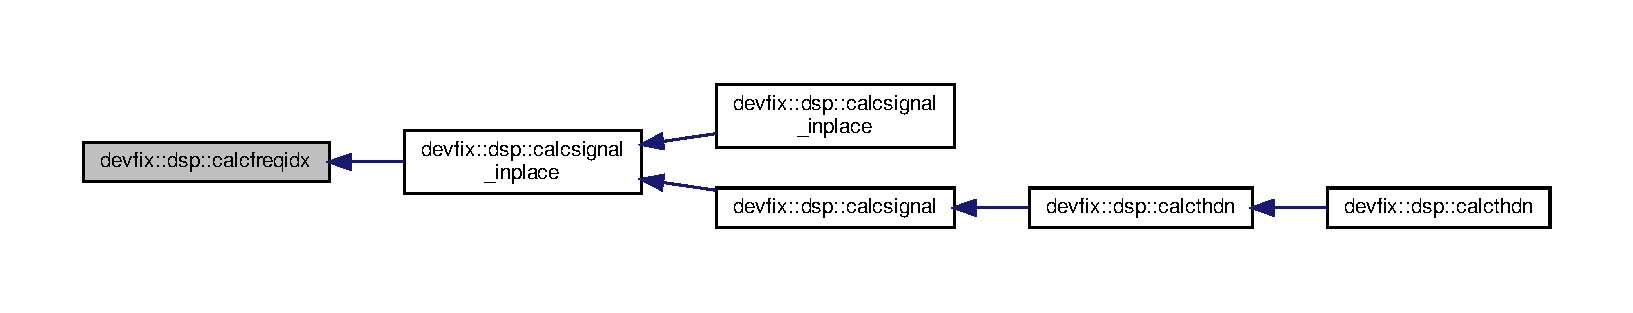
\includegraphics[width=350pt]{namespacedevfix_1_1dsp_a4c340dc6f142977c46850c3bd5467914_icgraph}
\end{center}
\end{figure}
\mbox{\Hypertarget{namespacedevfix_1_1dsp_acc73b4642ca4cb49621e76efc6732186}\label{namespacedevfix_1_1dsp_acc73b4642ca4cb49621e76efc6732186}} 
\index{devfix\+::dsp@{devfix\+::dsp}!calcmean@{calcmean}}
\index{calcmean@{calcmean}!devfix\+::dsp@{devfix\+::dsp}}
\subsubsection{\texorpdfstring{calcmean()}{calcmean()}\hspace{0.1cm}{\footnotesize\ttfamily [1/3]}}
{\footnotesize\ttfamily template$<$typename FloatT $>$ \\
FloatT devfix\+::dsp\+::calcmean (\begin{DoxyParamCaption}\item[{const FloatT $\ast$}]{field,  }\item[{std\+::size\+\_\+t}]{len }\end{DoxyParamCaption})}

Here is the caller graph for this function\+:
\nopagebreak
\begin{figure}[H]
\begin{center}
\leavevmode
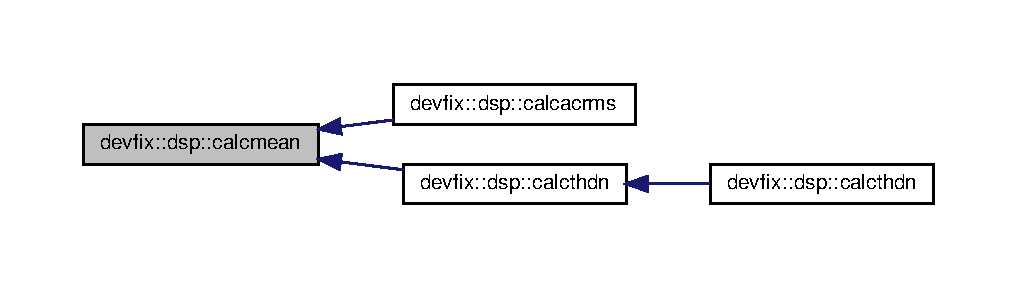
\includegraphics[width=350pt]{namespacedevfix_1_1dsp_acc73b4642ca4cb49621e76efc6732186_icgraph}
\end{center}
\end{figure}
\mbox{\Hypertarget{namespacedevfix_1_1dsp_ab8e51dea953cabfc246e2e45fbff010c}\label{namespacedevfix_1_1dsp_ab8e51dea953cabfc246e2e45fbff010c}} 
\index{devfix\+::dsp@{devfix\+::dsp}!calcmean@{calcmean}}
\index{calcmean@{calcmean}!devfix\+::dsp@{devfix\+::dsp}}
\subsubsection{\texorpdfstring{calcmean()}{calcmean()}\hspace{0.1cm}{\footnotesize\ttfamily [2/3]}}
{\footnotesize\ttfamily template$<$typename FloatT $>$ \\
FloatT devfix\+::dsp\+::calcmean (\begin{DoxyParamCaption}\item[{const std\+::vector$<$ FloatT $>$ \&}]{vec }\end{DoxyParamCaption})}

\mbox{\Hypertarget{namespacedevfix_1_1dsp_a9f44af4b1a42d61d8a52afb7a5628001}\label{namespacedevfix_1_1dsp_a9f44af4b1a42d61d8a52afb7a5628001}} 
\index{devfix\+::dsp@{devfix\+::dsp}!calcmean@{calcmean}}
\index{calcmean@{calcmean}!devfix\+::dsp@{devfix\+::dsp}}
\subsubsection{\texorpdfstring{calcmean()}{calcmean()}\hspace{0.1cm}{\footnotesize\ttfamily [3/3]}}
{\footnotesize\ttfamily template$<$typename FloatT , std\+::size\+\_\+t N$>$ \\
FloatT devfix\+::dsp\+::calcmean (\begin{DoxyParamCaption}\item[{const std\+::array$<$ FloatT, N $>$ \&}]{arr }\end{DoxyParamCaption})}

\mbox{\Hypertarget{namespacedevfix_1_1dsp_a3f84878d478c956e3dd2e4d0939a31e4}\label{namespacedevfix_1_1dsp_a3f84878d478c956e3dd2e4d0939a31e4}} 
\index{devfix\+::dsp@{devfix\+::dsp}!calcphasecorrector@{calcphasecorrector}}
\index{calcphasecorrector@{calcphasecorrector}!devfix\+::dsp@{devfix\+::dsp}}
\subsubsection{\texorpdfstring{calcphasecorrector()}{calcphasecorrector()}}
{\footnotesize\ttfamily template$<$typename FloatT $>$ \\
constexpr std\+::complex$<$FloatT$>$ devfix\+::dsp\+::calcphasecorrector (\begin{DoxyParamCaption}\item[{std\+::size\+\_\+t}]{sample\+\_\+rate,  }\item[{std\+::size\+\_\+t}]{fft\+\_\+len,  }\item[{FloatT}]{freq }\end{DoxyParamCaption})}



calculates the phase corrector factor for a non coherent frequency 


\begin{DoxyTemplParams}{Template Parameters}
{\em FloatT} & type for floating point numbers, determines precision \\
\hline
\end{DoxyTemplParams}

\begin{DoxyParams}{Parameters}
{\em sample\+\_\+rate} & \\
\hline
{\em fft\+\_\+len} & used fft length \\
\hline
{\em freq} & frequency of which the corrector factor gets calculated \\
\hline
\end{DoxyParams}
\begin{DoxyReturn}{Returns}

\end{DoxyReturn}
Here is the caller graph for this function\+:
\nopagebreak
\begin{figure}[H]
\begin{center}
\leavevmode
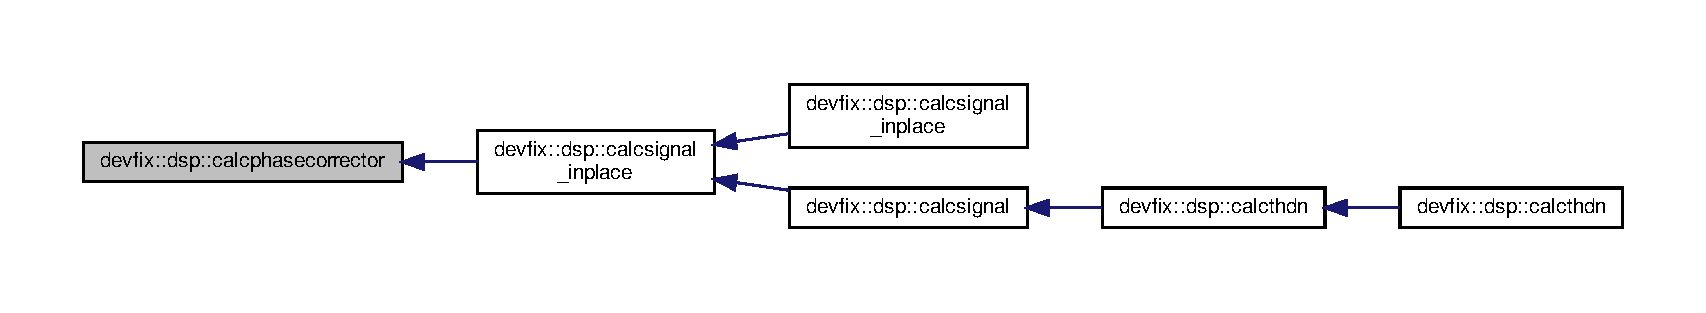
\includegraphics[width=350pt]{namespacedevfix_1_1dsp_a3f84878d478c956e3dd2e4d0939a31e4_icgraph}
\end{center}
\end{figure}
\mbox{\Hypertarget{namespacedevfix_1_1dsp_a1d758c2b667d7d48c41677641086387f}\label{namespacedevfix_1_1dsp_a1d758c2b667d7d48c41677641086387f}} 
\index{devfix\+::dsp@{devfix\+::dsp}!calcrms@{calcrms}}
\index{calcrms@{calcrms}!devfix\+::dsp@{devfix\+::dsp}}
\subsubsection{\texorpdfstring{calcrms()}{calcrms()}\hspace{0.1cm}{\footnotesize\ttfamily [1/3]}}
{\footnotesize\ttfamily template$<$typename FloatT $>$ \\
FloatT devfix\+::dsp\+::calcrms (\begin{DoxyParamCaption}\item[{const FloatT $\ast$}]{field,  }\item[{std\+::size\+\_\+t}]{len }\end{DoxyParamCaption})}

Here is the caller graph for this function\+:
\nopagebreak
\begin{figure}[H]
\begin{center}
\leavevmode
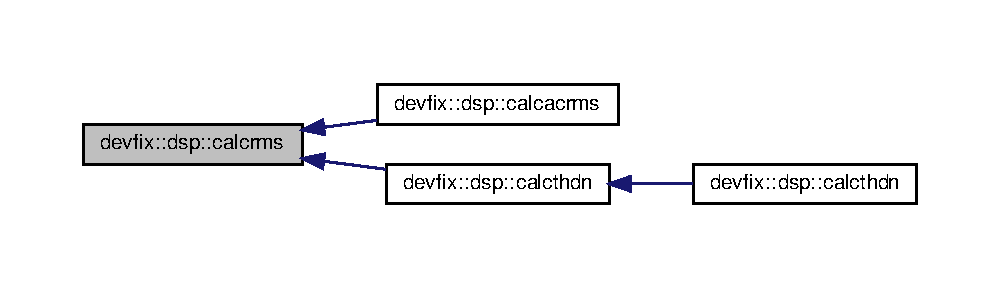
\includegraphics[width=350pt]{namespacedevfix_1_1dsp_a1d758c2b667d7d48c41677641086387f_icgraph}
\end{center}
\end{figure}
\mbox{\Hypertarget{namespacedevfix_1_1dsp_a18e7f97d5726a6273908d87a480446a5}\label{namespacedevfix_1_1dsp_a18e7f97d5726a6273908d87a480446a5}} 
\index{devfix\+::dsp@{devfix\+::dsp}!calcrms@{calcrms}}
\index{calcrms@{calcrms}!devfix\+::dsp@{devfix\+::dsp}}
\subsubsection{\texorpdfstring{calcrms()}{calcrms()}\hspace{0.1cm}{\footnotesize\ttfamily [2/3]}}
{\footnotesize\ttfamily template$<$typename FloatT $>$ \\
FloatT devfix\+::dsp\+::calcrms (\begin{DoxyParamCaption}\item[{const std\+::vector$<$ FloatT $>$ \&}]{vec }\end{DoxyParamCaption})}

\mbox{\Hypertarget{namespacedevfix_1_1dsp_a19c2e4d076954efbf0dab3daded46ba7}\label{namespacedevfix_1_1dsp_a19c2e4d076954efbf0dab3daded46ba7}} 
\index{devfix\+::dsp@{devfix\+::dsp}!calcrms@{calcrms}}
\index{calcrms@{calcrms}!devfix\+::dsp@{devfix\+::dsp}}
\subsubsection{\texorpdfstring{calcrms()}{calcrms()}\hspace{0.1cm}{\footnotesize\ttfamily [3/3]}}
{\footnotesize\ttfamily template$<$typename FloatT , std\+::size\+\_\+t N$>$ \\
FloatT devfix\+::dsp\+::calcrms (\begin{DoxyParamCaption}\item[{const std\+::array$<$ FloatT, N $>$ \&}]{arr }\end{DoxyParamCaption})}

\mbox{\Hypertarget{namespacedevfix_1_1dsp_a1dc562f09e21a538a14df82aaa083526}\label{namespacedevfix_1_1dsp_a1dc562f09e21a538a14df82aaa083526}} 
\index{devfix\+::dsp@{devfix\+::dsp}!calcsignal@{calcsignal}}
\index{calcsignal@{calcsignal}!devfix\+::dsp@{devfix\+::dsp}}
\subsubsection{\texorpdfstring{calcsignal()}{calcsignal()}\hspace{0.1cm}{\footnotesize\ttfamily [1/3]}}
{\footnotesize\ttfamily template$<$typename FloatT $>$ \\
std\+::complex$<$FloatT$>$ devfix\+::dsp\+::calcsignal (\begin{DoxyParamCaption}\item[{std\+::size\+\_\+t}]{sample\+\_\+rate,  }\item[{FloatT}]{freq,  }\item[{const FloatT $\ast$}]{field,  }\item[{std\+::size\+\_\+t}]{len }\end{DoxyParamCaption})}

Here is the caller graph for this function\+:
\nopagebreak
\begin{figure}[H]
\begin{center}
\leavevmode
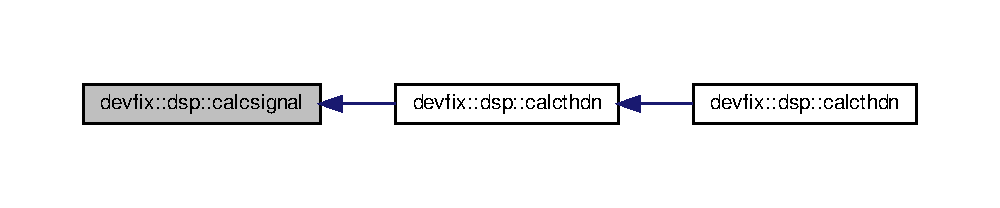
\includegraphics[width=350pt]{namespacedevfix_1_1dsp_a1dc562f09e21a538a14df82aaa083526_icgraph}
\end{center}
\end{figure}
\mbox{\Hypertarget{namespacedevfix_1_1dsp_aa8a0808fce2bd9ec139788f9d7fa7e59}\label{namespacedevfix_1_1dsp_aa8a0808fce2bd9ec139788f9d7fa7e59}} 
\index{devfix\+::dsp@{devfix\+::dsp}!calcsignal@{calcsignal}}
\index{calcsignal@{calcsignal}!devfix\+::dsp@{devfix\+::dsp}}
\subsubsection{\texorpdfstring{calcsignal()}{calcsignal()}\hspace{0.1cm}{\footnotesize\ttfamily [2/3]}}
{\footnotesize\ttfamily template$<$typename FloatT $>$ \\
std\+::complex$<$FloatT$>$ devfix\+::dsp\+::calcsignal (\begin{DoxyParamCaption}\item[{std\+::size\+\_\+t}]{sample\+\_\+rate,  }\item[{FloatT}]{freq,  }\item[{const std\+::vector$<$ FloatT $>$ \&}]{vec }\end{DoxyParamCaption})}

\mbox{\Hypertarget{namespacedevfix_1_1dsp_af2156150e070c8ec603f0134371187d4}\label{namespacedevfix_1_1dsp_af2156150e070c8ec603f0134371187d4}} 
\index{devfix\+::dsp@{devfix\+::dsp}!calcsignal@{calcsignal}}
\index{calcsignal@{calcsignal}!devfix\+::dsp@{devfix\+::dsp}}
\subsubsection{\texorpdfstring{calcsignal()}{calcsignal()}\hspace{0.1cm}{\footnotesize\ttfamily [3/3]}}
{\footnotesize\ttfamily template$<$typename FloatT , std\+::size\+\_\+t N$>$ \\
std\+::complex$<$FloatT$>$ devfix\+::dsp\+::calcsignal (\begin{DoxyParamCaption}\item[{std\+::size\+\_\+t}]{sample\+\_\+rate,  }\item[{FloatT}]{freq,  }\item[{const std\+::array$<$ FloatT, N $>$ \&}]{arr }\end{DoxyParamCaption})}

\mbox{\Hypertarget{namespacedevfix_1_1dsp_a38dc66c795b9ebe6e8408d95c7a006c9}\label{namespacedevfix_1_1dsp_a38dc66c795b9ebe6e8408d95c7a006c9}} 
\index{devfix\+::dsp@{devfix\+::dsp}!calcsignal\+\_\+inplace@{calcsignal\+\_\+inplace}}
\index{calcsignal\+\_\+inplace@{calcsignal\+\_\+inplace}!devfix\+::dsp@{devfix\+::dsp}}
\subsubsection{\texorpdfstring{calcsignal\+\_\+inplace()}{calcsignal\_inplace()}\hspace{0.1cm}{\footnotesize\ttfamily [1/3]}}
{\footnotesize\ttfamily template$<$typename FloatT $>$ \\
std\+::complex$<$FloatT$>$ devfix\+::dsp\+::calcsignal\+\_\+inplace (\begin{DoxyParamCaption}\item[{std\+::size\+\_\+t}]{sample\+\_\+rate,  }\item[{FloatT}]{freq,  }\item[{std\+::complex$<$ FloatT $>$ $\ast$}]{field,  }\item[{std\+::size\+\_\+t}]{len }\end{DoxyParamCaption})}

Here is the caller graph for this function\+:
\nopagebreak
\begin{figure}[H]
\begin{center}
\leavevmode
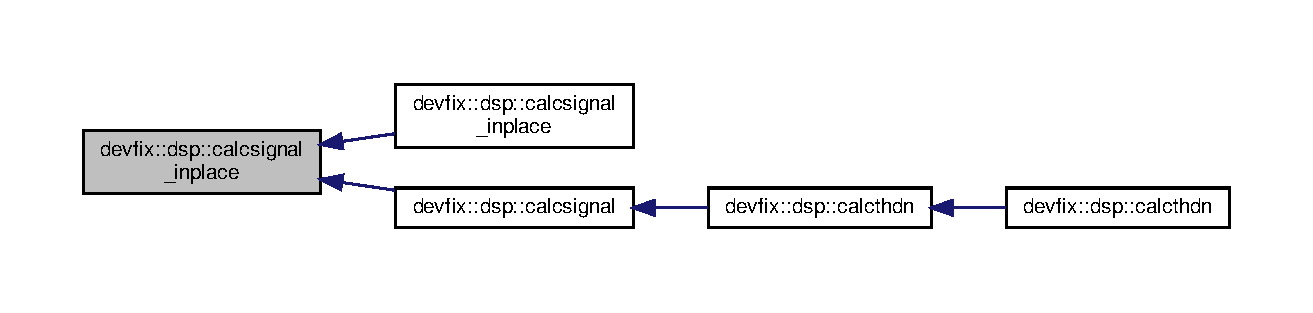
\includegraphics[width=350pt]{namespacedevfix_1_1dsp_a38dc66c795b9ebe6e8408d95c7a006c9_icgraph}
\end{center}
\end{figure}
\mbox{\Hypertarget{namespacedevfix_1_1dsp_af2bf29501002d08830f1a7ac3ff22289}\label{namespacedevfix_1_1dsp_af2bf29501002d08830f1a7ac3ff22289}} 
\index{devfix\+::dsp@{devfix\+::dsp}!calcsignal\+\_\+inplace@{calcsignal\+\_\+inplace}}
\index{calcsignal\+\_\+inplace@{calcsignal\+\_\+inplace}!devfix\+::dsp@{devfix\+::dsp}}
\subsubsection{\texorpdfstring{calcsignal\+\_\+inplace()}{calcsignal\_inplace()}\hspace{0.1cm}{\footnotesize\ttfamily [2/3]}}
{\footnotesize\ttfamily template$<$typename FloatT $>$ \\
std\+::complex$<$FloatT$>$ devfix\+::dsp\+::calcsignal\+\_\+inplace (\begin{DoxyParamCaption}\item[{std\+::size\+\_\+t}]{sample\+\_\+rate,  }\item[{FloatT}]{freq,  }\item[{std\+::vector$<$ std\+::complex$<$ FloatT $>$$>$ \&}]{vec }\end{DoxyParamCaption})}

\mbox{\Hypertarget{namespacedevfix_1_1dsp_ab4671999093ac0b52a1f3fdce063750d}\label{namespacedevfix_1_1dsp_ab4671999093ac0b52a1f3fdce063750d}} 
\index{devfix\+::dsp@{devfix\+::dsp}!calcsignal\+\_\+inplace@{calcsignal\+\_\+inplace}}
\index{calcsignal\+\_\+inplace@{calcsignal\+\_\+inplace}!devfix\+::dsp@{devfix\+::dsp}}
\subsubsection{\texorpdfstring{calcsignal\+\_\+inplace()}{calcsignal\_inplace()}\hspace{0.1cm}{\footnotesize\ttfamily [3/3]}}
{\footnotesize\ttfamily template$<$typename FloatT , std\+::size\+\_\+t N$>$ \\
std\+::complex$<$FloatT$>$ devfix\+::dsp\+::calcsignal\+\_\+inplace (\begin{DoxyParamCaption}\item[{std\+::size\+\_\+t}]{sample\+\_\+rate,  }\item[{FloatT}]{freq,  }\item[{std\+::array$<$ std\+::complex$<$ FloatT $>$, N $>$ \&}]{arr }\end{DoxyParamCaption})}

\mbox{\Hypertarget{namespacedevfix_1_1dsp_a1982c6b562b8c196dd3322c207c0ac86}\label{namespacedevfix_1_1dsp_a1982c6b562b8c196dd3322c207c0ac86}} 
\index{devfix\+::dsp@{devfix\+::dsp}!calcthdn@{calcthdn}}
\index{calcthdn@{calcthdn}!devfix\+::dsp@{devfix\+::dsp}}
\subsubsection{\texorpdfstring{calcthdn()}{calcthdn()}\hspace{0.1cm}{\footnotesize\ttfamily [1/3]}}
{\footnotesize\ttfamily template$<$typename FloatT $>$ \\
FloatT devfix\+::dsp\+::calcthdn (\begin{DoxyParamCaption}\item[{std\+::size\+\_\+t}]{sample\+\_\+rate,  }\item[{FloatT}]{freq,  }\item[{const FloatT $\ast$}]{field,  }\item[{std\+::size\+\_\+t}]{len }\end{DoxyParamCaption})}

Here is the caller graph for this function\+:
\nopagebreak
\begin{figure}[H]
\begin{center}
\leavevmode
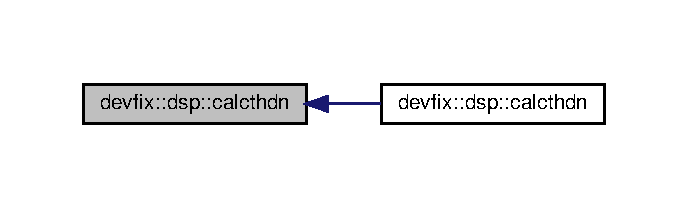
\includegraphics[width=330pt]{namespacedevfix_1_1dsp_a1982c6b562b8c196dd3322c207c0ac86_icgraph}
\end{center}
\end{figure}
\mbox{\Hypertarget{namespacedevfix_1_1dsp_a424b6903cca9ea1aebfa4712ea070a1e}\label{namespacedevfix_1_1dsp_a424b6903cca9ea1aebfa4712ea070a1e}} 
\index{devfix\+::dsp@{devfix\+::dsp}!calcthdn@{calcthdn}}
\index{calcthdn@{calcthdn}!devfix\+::dsp@{devfix\+::dsp}}
\subsubsection{\texorpdfstring{calcthdn()}{calcthdn()}\hspace{0.1cm}{\footnotesize\ttfamily [2/3]}}
{\footnotesize\ttfamily template$<$typename FloatT $>$ \\
FloatT devfix\+::dsp\+::calcthdn (\begin{DoxyParamCaption}\item[{std\+::size\+\_\+t}]{sample\+\_\+rate,  }\item[{FloatT}]{freq,  }\item[{const std\+::vector$<$ FloatT $>$ \&}]{vec }\end{DoxyParamCaption})}

\mbox{\Hypertarget{namespacedevfix_1_1dsp_a54194236560fd3dd40df38df44966d8e}\label{namespacedevfix_1_1dsp_a54194236560fd3dd40df38df44966d8e}} 
\index{devfix\+::dsp@{devfix\+::dsp}!calcthdn@{calcthdn}}
\index{calcthdn@{calcthdn}!devfix\+::dsp@{devfix\+::dsp}}
\subsubsection{\texorpdfstring{calcthdn()}{calcthdn()}\hspace{0.1cm}{\footnotesize\ttfamily [3/3]}}
{\footnotesize\ttfamily template$<$typename FloatT , std\+::size\+\_\+t N$>$ \\
FloatT devfix\+::dsp\+::calcthdn (\begin{DoxyParamCaption}\item[{std\+::size\+\_\+t}]{sample\+\_\+rate,  }\item[{FloatT}]{freq,  }\item[{const std\+::array$<$ FloatT, N $>$ \&}]{arr }\end{DoxyParamCaption})}

\mbox{\Hypertarget{namespacedevfix_1_1dsp_a5e776756816f3429899134f5c8b8b215}\label{namespacedevfix_1_1dsp_a5e776756816f3429899134f5c8b8b215}} 
\index{devfix\+::dsp@{devfix\+::dsp}!goertzel@{goertzel}}
\index{goertzel@{goertzel}!devfix\+::dsp@{devfix\+::dsp}}
\subsubsection{\texorpdfstring{goertzel()}{goertzel()}\hspace{0.1cm}{\footnotesize\ttfamily [1/3]}}
{\footnotesize\ttfamily template$<$typename FloatT $>$ \\
std\+::complex$<$FloatT$>$ devfix\+::dsp\+::goertzel (\begin{DoxyParamCaption}\item[{const std\+::complex$<$ FloatT $>$ $\ast$}]{field,  }\item[{std\+::size\+\_\+t}]{len,  }\item[{std\+::size\+\_\+t}]{k }\end{DoxyParamCaption})}



calculates an dft coefficient of the discrete Fourier-\/transformation 


\begin{DoxyTemplParams}{Template Parameters}
{\em FloatT} & floating point type \\
\hline
\end{DoxyTemplParams}

\begin{DoxyParams}{Parameters}
{\em field} & \\
\hline
{\em len} & \\
\hline
{\em k} & \\
\hline
\end{DoxyParams}
\begin{DoxyReturn}{Returns}

\end{DoxyReturn}
Here is the caller graph for this function\+:
\nopagebreak
\begin{figure}[H]
\begin{center}
\leavevmode
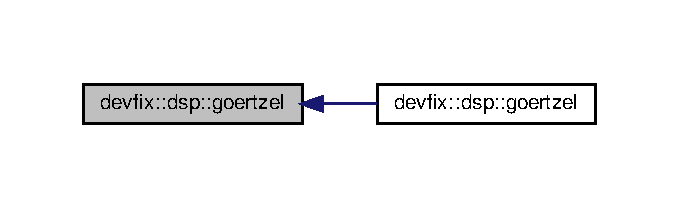
\includegraphics[width=350pt]{namespacedevfix_1_1dsp_a5e776756816f3429899134f5c8b8b215_icgraph}
\end{center}
\end{figure}
\mbox{\Hypertarget{namespacedevfix_1_1dsp_a9c0640ca74af740499f9c3da2019930c}\label{namespacedevfix_1_1dsp_a9c0640ca74af740499f9c3da2019930c}} 
\index{devfix\+::dsp@{devfix\+::dsp}!goertzel@{goertzel}}
\index{goertzel@{goertzel}!devfix\+::dsp@{devfix\+::dsp}}
\subsubsection{\texorpdfstring{goertzel()}{goertzel()}\hspace{0.1cm}{\footnotesize\ttfamily [2/3]}}
{\footnotesize\ttfamily template$<$typename FloatT $>$ \\
std\+::complex$<$FloatT$>$ devfix\+::dsp\+::goertzel (\begin{DoxyParamCaption}\item[{const std\+::vector$<$ std\+::complex$<$ FloatT $>$$>$ \&}]{vec,  }\item[{std\+::size\+\_\+t}]{k }\end{DoxyParamCaption})}

\mbox{\Hypertarget{namespacedevfix_1_1dsp_a3eed4648161700e03c0f6d900bea9f73}\label{namespacedevfix_1_1dsp_a3eed4648161700e03c0f6d900bea9f73}} 
\index{devfix\+::dsp@{devfix\+::dsp}!goertzel@{goertzel}}
\index{goertzel@{goertzel}!devfix\+::dsp@{devfix\+::dsp}}
\subsubsection{\texorpdfstring{goertzel()}{goertzel()}\hspace{0.1cm}{\footnotesize\ttfamily [3/3]}}
{\footnotesize\ttfamily template$<$typename FloatT , std\+::size\+\_\+t N$>$ \\
std\+::complex$<$FloatT$>$ devfix\+::dsp\+::goertzel (\begin{DoxyParamCaption}\item[{const std\+::array$<$ std\+::complex$<$ FloatT $>$, N $>$ \&}]{arr,  }\item[{std\+::size\+\_\+t}]{k }\end{DoxyParamCaption})}


\hypertarget{namespacedevfix_1_1net}{}\section{devfix\+:\+:net Namespace Reference}
\label{namespacedevfix_1_1net}\index{devfix\+::net@{devfix\+::net}}
\subsection*{Classes}
\begin{DoxyCompactItemize}
\item 
struct \hyperlink{structdevfix_1_1net_1_1inetaddress}{inetaddress}
\item 
struct \hyperlink{structdevfix_1_1net_1_1netbuilder}{netbuilder}
\item 
struct \hyperlink{structdevfix_1_1net_1_1serversocket}{serversocket}
\item 
struct \hyperlink{structdevfix_1_1net_1_1socket}{socket}
\item 
struct \hyperlink{structdevfix_1_1net_1_1socketexception}{socketexception}
\begin{DoxyCompactList}\small\item\em Thrown to indicate that there is an error creating or accessing a Socket. \end{DoxyCompactList}\end{DoxyCompactItemize}

\chapter{Class Documentation}
\hypertarget{structdevfix_1_1base_1_1error_1_1baseexception}{}\section{devfix\+:\+:base\+:\+:error\+:\+:baseexception Struct Reference}
\label{structdevfix_1_1base_1_1error_1_1baseexception}\index{devfix\+::base\+::error\+::baseexception@{devfix\+::base\+::error\+::baseexception}}


Abstract error base class.  




{\ttfamily \#include $<$baseexception.\+h$>$}



Inheritance diagram for devfix\+:\+:base\+:\+:error\+:\+:baseexception\+:

\hypertarget{structdevfix_1_1dsp_1_1window_1_1buffer}{}\section{devfix\+:\+:dsp\+:\+:window\+:\+:buffer$<$ FloatT, win\+\_\+fun $>$ Struct Template Reference}
\label{structdevfix_1_1dsp_1_1window_1_1buffer}\index{devfix\+::dsp\+::window\+::buffer$<$ Float\+T, win\+\_\+fun $>$@{devfix\+::dsp\+::window\+::buffer$<$ Float\+T, win\+\_\+fun $>$}}


{\ttfamily \#include $<$window.\+h$>$}

\subsection*{Static Public Member Functions}
\begin{DoxyCompactItemize}
\item 
static const std\+::vector$<$ FloatT $>$ \& \hyperlink{structdevfix_1_1dsp_1_1window_1_1buffer_a3ace062676326a9981118d53b8ba5900}{prepare} (std\+::size\+\_\+t n)
\item 
static void \hyperlink{structdevfix_1_1dsp_1_1window_1_1buffer_a525423f47082a367abe172a6ac61e65d}{clear} ()
\item 
static std\+::size\+\_\+t \hyperlink{structdevfix_1_1dsp_1_1window_1_1buffer_af1215d236069b0848e7211e5f697b3fa}{size} ()
\item 
static FloatT \hyperlink{structdevfix_1_1dsp_1_1window_1_1buffer_a877f872e06b4709189e15c38f247445f}{get\+\_\+window} (std\+::size\+\_\+t n, std\+::size\+\_\+t k)
\end{DoxyCompactItemize}


\subsection{Member Function Documentation}
\mbox{\Hypertarget{structdevfix_1_1dsp_1_1window_1_1buffer_a525423f47082a367abe172a6ac61e65d}\label{structdevfix_1_1dsp_1_1window_1_1buffer_a525423f47082a367abe172a6ac61e65d}} 
\index{devfix\+::dsp\+::window\+::buffer@{devfix\+::dsp\+::window\+::buffer}!clear@{clear}}
\index{clear@{clear}!devfix\+::dsp\+::window\+::buffer@{devfix\+::dsp\+::window\+::buffer}}
\subsubsection{\texorpdfstring{clear()}{clear()}}
{\footnotesize\ttfamily template$<$typename FloatT , win\+\_\+fun\+\_\+t$<$ Float\+T $>$ win\+\_\+fun$>$ \\
static void \hyperlink{structdevfix_1_1dsp_1_1window_1_1buffer}{devfix\+::dsp\+::window\+::buffer}$<$ FloatT, win\+\_\+fun $>$\+::clear (\begin{DoxyParamCaption}{ }\end{DoxyParamCaption})\hspace{0.3cm}{\ttfamily [inline]}, {\ttfamily [static]}}

\mbox{\Hypertarget{structdevfix_1_1dsp_1_1window_1_1buffer_a877f872e06b4709189e15c38f247445f}\label{structdevfix_1_1dsp_1_1window_1_1buffer_a877f872e06b4709189e15c38f247445f}} 
\index{devfix\+::dsp\+::window\+::buffer@{devfix\+::dsp\+::window\+::buffer}!get\+\_\+window@{get\+\_\+window}}
\index{get\+\_\+window@{get\+\_\+window}!devfix\+::dsp\+::window\+::buffer@{devfix\+::dsp\+::window\+::buffer}}
\subsubsection{\texorpdfstring{get\+\_\+window()}{get\_window()}}
{\footnotesize\ttfamily template$<$typename FloatT , win\+\_\+fun\+\_\+t$<$ Float\+T $>$ win\+\_\+fun$>$ \\
static FloatT \hyperlink{structdevfix_1_1dsp_1_1window_1_1buffer}{devfix\+::dsp\+::window\+::buffer}$<$ FloatT, win\+\_\+fun $>$\+::get\+\_\+window (\begin{DoxyParamCaption}\item[{std\+::size\+\_\+t}]{n,  }\item[{std\+::size\+\_\+t}]{k }\end{DoxyParamCaption})\hspace{0.3cm}{\ttfamily [inline]}, {\ttfamily [static]}}

\mbox{\Hypertarget{structdevfix_1_1dsp_1_1window_1_1buffer_a3ace062676326a9981118d53b8ba5900}\label{structdevfix_1_1dsp_1_1window_1_1buffer_a3ace062676326a9981118d53b8ba5900}} 
\index{devfix\+::dsp\+::window\+::buffer@{devfix\+::dsp\+::window\+::buffer}!prepare@{prepare}}
\index{prepare@{prepare}!devfix\+::dsp\+::window\+::buffer@{devfix\+::dsp\+::window\+::buffer}}
\subsubsection{\texorpdfstring{prepare()}{prepare()}}
{\footnotesize\ttfamily template$<$typename FloatT , win\+\_\+fun\+\_\+t$<$ Float\+T $>$ win\+\_\+fun$>$ \\
static const std\+::vector$<$FloatT$>$\& \hyperlink{structdevfix_1_1dsp_1_1window_1_1buffer}{devfix\+::dsp\+::window\+::buffer}$<$ FloatT, win\+\_\+fun $>$\+::prepare (\begin{DoxyParamCaption}\item[{std\+::size\+\_\+t}]{n }\end{DoxyParamCaption})\hspace{0.3cm}{\ttfamily [inline]}, {\ttfamily [static]}}

Here is the caller graph for this function\+:\nopagebreak
\begin{figure}[H]
\begin{center}
\leavevmode
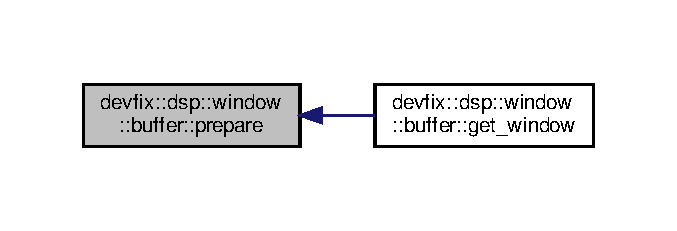
\includegraphics[width=325pt]{structdevfix_1_1dsp_1_1window_1_1buffer_a3ace062676326a9981118d53b8ba5900_icgraph}
\end{center}
\end{figure}
\mbox{\Hypertarget{structdevfix_1_1dsp_1_1window_1_1buffer_af1215d236069b0848e7211e5f697b3fa}\label{structdevfix_1_1dsp_1_1window_1_1buffer_af1215d236069b0848e7211e5f697b3fa}} 
\index{devfix\+::dsp\+::window\+::buffer@{devfix\+::dsp\+::window\+::buffer}!size@{size}}
\index{size@{size}!devfix\+::dsp\+::window\+::buffer@{devfix\+::dsp\+::window\+::buffer}}
\subsubsection{\texorpdfstring{size()}{size()}}
{\footnotesize\ttfamily template$<$typename FloatT , win\+\_\+fun\+\_\+t$<$ Float\+T $>$ win\+\_\+fun$>$ \\
static std\+::size\+\_\+t \hyperlink{structdevfix_1_1dsp_1_1window_1_1buffer}{devfix\+::dsp\+::window\+::buffer}$<$ FloatT, win\+\_\+fun $>$\+::size (\begin{DoxyParamCaption}{ }\end{DoxyParamCaption})\hspace{0.3cm}{\ttfamily [inline]}, {\ttfamily [static]}}



The documentation for this struct was generated from the following file\+:\begin{DoxyCompactItemize}
\item 
devfix/dsp/\hyperlink{window_8h}{window.\+h}\end{DoxyCompactItemize}

\hypertarget{structdevfix_1_1dsp_1_1fft}{}\section{devfix\+:\+:dsp\+:\+:fft Struct Reference}
\label{structdevfix_1_1dsp_1_1fft}\index{devfix\+::dsp\+::fft@{devfix\+::dsp\+::fft}}


{\ttfamily \#include $<$fft.\+h$>$}

\subsection*{Public Types}
\begin{DoxyCompactItemize}
\item 
using \hyperlink{structdevfix_1_1dsp_1_1fft_a6309eb88cede0b11f17067f8892af91a}{math} = \+::\hyperlink{structdevfix_1_1base_1_1math}{devfix\+::base\+::math}
\end{DoxyCompactItemize}
\subsection*{Static Public Member Functions}
\begin{DoxyCompactItemize}
\item 
{\footnotesize template$<$typename FloatT $>$ }\\static void \hyperlink{structdevfix_1_1dsp_1_1fft_a8e6e4580cc075ebaa7be5d2781a8e3eb}{transform\+\_\+inplace} (std\+::complex$<$ FloatT $>$ $\ast$field, std\+::size\+\_\+t len)
\begin{DoxyCompactList}\small\item\em performs the inplace discrete-\/fourier-\/transformation for an complex field, the field length has to be a power of two \end{DoxyCompactList}\item 
{\footnotesize template$<$typename FloatT $>$ }\\static void \hyperlink{structdevfix_1_1dsp_1_1fft_a3f9d520b7ee8f9fe233bbed45f0c10d8}{transform\+\_\+inplace} (std\+::vector$<$ std\+::complex$<$ FloatT $>$$>$ \&vec)
\begin{DoxyCompactList}\small\item\em performs the inplace discrete-\/fourier-\/transformation for an complex vector, the vector length has to be a power of two \end{DoxyCompactList}\item 
{\footnotesize template$<$typename FloatT , std\+::size\+\_\+t N$>$ }\\static void \hyperlink{structdevfix_1_1dsp_1_1fft_a92d4ff21f87fd2d1607c60788158cf62}{transform\+\_\+inplace} (std\+::array$<$ std\+::complex$<$ FloatT $>$, N $>$ \&arr)
\begin{DoxyCompactList}\small\item\em performs the inplace discrete-\/fourier-\/transformation for an complex array, the array length has to be a power of two \end{DoxyCompactList}\item 
{\footnotesize template$<$typename FloatT $>$ }\\static void \hyperlink{structdevfix_1_1dsp_1_1fft_ac05e043eb9375c77ff7e4ab5843d82af}{normalize\+\_\+inplace} (std\+::complex$<$ FloatT $>$ $\ast$field, std\+::size\+\_\+t len, std\+::size\+\_\+t n=0)
\begin{DoxyCompactList}\small\item\em divides each element of the field by the fft size, if the fft size is zero, it gets set to the field length \end{DoxyCompactList}\item 
{\footnotesize template$<$typename FloatT $>$ }\\static void \hyperlink{structdevfix_1_1dsp_1_1fft_af4e943d0958fc382656380ca2bc993cc}{normalize\+\_\+inplace} (std\+::vector$<$ std\+::complex$<$ FloatT $>$$>$ \&vec, std\+::size\+\_\+t n=0)
\begin{DoxyCompactList}\small\item\em divides each element of the vector by the fft size, if the fft size is zero, it gets set to the vector size \end{DoxyCompactList}\item 
{\footnotesize template$<$typename FloatT , std\+::size\+\_\+t N$>$ }\\static void \hyperlink{structdevfix_1_1dsp_1_1fft_a7b52c39390680041aa9800295f310f9d}{normalize\+\_\+inplace} (std\+::array$<$ std\+::complex$<$ FloatT $>$, N $>$ \&arr, std\+::size\+\_\+t n=0)
\begin{DoxyCompactList}\small\item\em divides each element of the array by the fft size, if the fft size is zero, it gets set to the array size \end{DoxyCompactList}\item 
{\footnotesize template$<$typename FloatT $>$ }\\static void \hyperlink{structdevfix_1_1dsp_1_1fft_a5e56000eec31a31dc7a2fc7af198b709}{get\+\_\+magnitude} (const std\+::complex$<$ FloatT $>$ $\ast$field, std\+::size\+\_\+t len, FloatT $\ast$mag)
\begin{DoxyCompactList}\small\item\em calculates the magnitudes of a normalized fft field \end{DoxyCompactList}\item 
{\footnotesize template$<$typename FloatT $>$ }\\static std\+::vector$<$ FloatT $>$ \hyperlink{structdevfix_1_1dsp_1_1fft_a9c937104cad67dd01f56870e44dd9556}{get\+\_\+magnitude} (const std\+::vector$<$ std\+::complex$<$ FloatT $>$$>$ \&vec)
\begin{DoxyCompactList}\small\item\em calculates the magnitudes of a normalized fft vector \end{DoxyCompactList}\item 
{\footnotesize template$<$typename FloatT , std\+::size\+\_\+t N$>$ }\\static std\+::array$<$ FloatT, N/2 $>$ \hyperlink{structdevfix_1_1dsp_1_1fft_aca37b18e5e6352088d9f24a71a6e3573}{get\+\_\+magnitude} (const std\+::array$<$ std\+::complex$<$ FloatT $>$, N $>$ \&arr)
\begin{DoxyCompactList}\small\item\em calculates the magnitudes of a normalized fft vector \end{DoxyCompactList}\item 
{\footnotesize template$<$typename FloatT $>$ }\\static void \hyperlink{structdevfix_1_1dsp_1_1fft_a330303a45a2dfd49d19fff95d9cf14cd}{get\+\_\+phase} (const std\+::complex$<$ FloatT $>$ $\ast$field, std\+::size\+\_\+t len, FloatT $\ast$ph)
\begin{DoxyCompactList}\small\item\em calculates the phases of a normalized fft field \end{DoxyCompactList}\item 
{\footnotesize template$<$typename FloatT $>$ }\\static std\+::vector$<$ FloatT $>$ \hyperlink{structdevfix_1_1dsp_1_1fft_a3efcfd1a671e6558cf7ca25379317ada}{get\+\_\+phase} (const std\+::vector$<$ std\+::complex$<$ FloatT $>$$>$ \&vec)
\begin{DoxyCompactList}\small\item\em calculates the phases of a normalized fft vector \end{DoxyCompactList}\item 
{\footnotesize template$<$typename FloatT , std\+::size\+\_\+t N$>$ }\\static std\+::array$<$ FloatT, N/2 $>$ \hyperlink{structdevfix_1_1dsp_1_1fft_abee685e0c6688e55a353ca019ea2793c}{get\+\_\+phase} (const std\+::array$<$ std\+::complex$<$ FloatT $>$, N $>$ \&arr)
\begin{DoxyCompactList}\small\item\em calculates the phases of a normalized fft array \end{DoxyCompactList}\end{DoxyCompactItemize}


\subsection{Member Typedef Documentation}
\mbox{\Hypertarget{structdevfix_1_1dsp_1_1fft_a6309eb88cede0b11f17067f8892af91a}\label{structdevfix_1_1dsp_1_1fft_a6309eb88cede0b11f17067f8892af91a}} 
\index{devfix\+::dsp\+::fft@{devfix\+::dsp\+::fft}!math@{math}}
\index{math@{math}!devfix\+::dsp\+::fft@{devfix\+::dsp\+::fft}}
\subsubsection{\texorpdfstring{math}{math}}
{\footnotesize\ttfamily using \hyperlink{structdevfix_1_1dsp_1_1fft_a6309eb88cede0b11f17067f8892af91a}{devfix\+::dsp\+::fft\+::math} =  \+::\hyperlink{structdevfix_1_1base_1_1math}{devfix\+::base\+::math}}



\subsection{Member Function Documentation}
\mbox{\Hypertarget{structdevfix_1_1dsp_1_1fft_a5e56000eec31a31dc7a2fc7af198b709}\label{structdevfix_1_1dsp_1_1fft_a5e56000eec31a31dc7a2fc7af198b709}} 
\index{devfix\+::dsp\+::fft@{devfix\+::dsp\+::fft}!get\+\_\+magnitude@{get\+\_\+magnitude}}
\index{get\+\_\+magnitude@{get\+\_\+magnitude}!devfix\+::dsp\+::fft@{devfix\+::dsp\+::fft}}
\subsubsection{\texorpdfstring{get\+\_\+magnitude()}{get\_magnitude()}\hspace{0.1cm}{\footnotesize\ttfamily [1/3]}}
{\footnotesize\ttfamily template$<$typename FloatT $>$ \\
static void devfix\+::dsp\+::fft\+::get\+\_\+magnitude (\begin{DoxyParamCaption}\item[{const std\+::complex$<$ FloatT $>$ $\ast$}]{field,  }\item[{std\+::size\+\_\+t}]{len,  }\item[{FloatT $\ast$}]{mag }\end{DoxyParamCaption})\hspace{0.3cm}{\ttfamily [inline]}, {\ttfamily [static]}}



calculates the magnitudes of a normalized fft field 


\begin{DoxyTemplParams}{Template Parameters}
{\em FloatT} & type of floating point numbers \\
\hline
\end{DoxyTemplParams}

\begin{DoxyParams}{Parameters}
{\em field} & input field \\
\hline
{\em len} & input field length \\
\hline
{\em mag} & output field for the magnitudes \\
\hline
\end{DoxyParams}
\mbox{\Hypertarget{structdevfix_1_1dsp_1_1fft_a9c937104cad67dd01f56870e44dd9556}\label{structdevfix_1_1dsp_1_1fft_a9c937104cad67dd01f56870e44dd9556}} 
\index{devfix\+::dsp\+::fft@{devfix\+::dsp\+::fft}!get\+\_\+magnitude@{get\+\_\+magnitude}}
\index{get\+\_\+magnitude@{get\+\_\+magnitude}!devfix\+::dsp\+::fft@{devfix\+::dsp\+::fft}}
\subsubsection{\texorpdfstring{get\+\_\+magnitude()}{get\_magnitude()}\hspace{0.1cm}{\footnotesize\ttfamily [2/3]}}
{\footnotesize\ttfamily template$<$typename FloatT $>$ \\
static std\+::vector$<$FloatT$>$ devfix\+::dsp\+::fft\+::get\+\_\+magnitude (\begin{DoxyParamCaption}\item[{const std\+::vector$<$ std\+::complex$<$ FloatT $>$$>$ \&}]{vec }\end{DoxyParamCaption})\hspace{0.3cm}{\ttfamily [inline]}, {\ttfamily [static]}}



calculates the magnitudes of a normalized fft vector 


\begin{DoxyTemplParams}{Template Parameters}
{\em FloatT} & type of floating point numbers \\
\hline
\end{DoxyTemplParams}

\begin{DoxyParams}{Parameters}
{\em vec} & input vector \\
\hline
\end{DoxyParams}
\begin{DoxyReturn}{Returns}
output vector with magnitudes 
\end{DoxyReturn}
\mbox{\Hypertarget{structdevfix_1_1dsp_1_1fft_aca37b18e5e6352088d9f24a71a6e3573}\label{structdevfix_1_1dsp_1_1fft_aca37b18e5e6352088d9f24a71a6e3573}} 
\index{devfix\+::dsp\+::fft@{devfix\+::dsp\+::fft}!get\+\_\+magnitude@{get\+\_\+magnitude}}
\index{get\+\_\+magnitude@{get\+\_\+magnitude}!devfix\+::dsp\+::fft@{devfix\+::dsp\+::fft}}
\subsubsection{\texorpdfstring{get\+\_\+magnitude()}{get\_magnitude()}\hspace{0.1cm}{\footnotesize\ttfamily [3/3]}}
{\footnotesize\ttfamily template$<$typename FloatT , std\+::size\+\_\+t N$>$ \\
static std\+::array$<$FloatT, N / 2$>$ devfix\+::dsp\+::fft\+::get\+\_\+magnitude (\begin{DoxyParamCaption}\item[{const std\+::array$<$ std\+::complex$<$ FloatT $>$, N $>$ \&}]{arr }\end{DoxyParamCaption})\hspace{0.3cm}{\ttfamily [inline]}, {\ttfamily [static]}}



calculates the magnitudes of a normalized fft vector 


\begin{DoxyTemplParams}{Template Parameters}
{\em FloatT} & type of floating point numbers \\
\hline
{\em N} & input array length \\
\hline
\end{DoxyTemplParams}

\begin{DoxyParams}{Parameters}
{\em arr} & input array \\
\hline
\end{DoxyParams}
\begin{DoxyReturn}{Returns}
output array with magnitudes 
\end{DoxyReturn}
\mbox{\Hypertarget{structdevfix_1_1dsp_1_1fft_a330303a45a2dfd49d19fff95d9cf14cd}\label{structdevfix_1_1dsp_1_1fft_a330303a45a2dfd49d19fff95d9cf14cd}} 
\index{devfix\+::dsp\+::fft@{devfix\+::dsp\+::fft}!get\+\_\+phase@{get\+\_\+phase}}
\index{get\+\_\+phase@{get\+\_\+phase}!devfix\+::dsp\+::fft@{devfix\+::dsp\+::fft}}
\subsubsection{\texorpdfstring{get\+\_\+phase()}{get\_phase()}\hspace{0.1cm}{\footnotesize\ttfamily [1/3]}}
{\footnotesize\ttfamily template$<$typename FloatT $>$ \\
static void devfix\+::dsp\+::fft\+::get\+\_\+phase (\begin{DoxyParamCaption}\item[{const std\+::complex$<$ FloatT $>$ $\ast$}]{field,  }\item[{std\+::size\+\_\+t}]{len,  }\item[{FloatT $\ast$}]{ph }\end{DoxyParamCaption})\hspace{0.3cm}{\ttfamily [inline]}, {\ttfamily [static]}}



calculates the phases of a normalized fft field 


\begin{DoxyTemplParams}{Template Parameters}
{\em FloatT} & type of floating point numbers \\
\hline
\end{DoxyTemplParams}

\begin{DoxyParams}{Parameters}
{\em field} & input field \\
\hline
{\em len} & input field length \\
\hline
{\em ph} & output field for the phases \\
\hline
\end{DoxyParams}
\mbox{\Hypertarget{structdevfix_1_1dsp_1_1fft_a3efcfd1a671e6558cf7ca25379317ada}\label{structdevfix_1_1dsp_1_1fft_a3efcfd1a671e6558cf7ca25379317ada}} 
\index{devfix\+::dsp\+::fft@{devfix\+::dsp\+::fft}!get\+\_\+phase@{get\+\_\+phase}}
\index{get\+\_\+phase@{get\+\_\+phase}!devfix\+::dsp\+::fft@{devfix\+::dsp\+::fft}}
\subsubsection{\texorpdfstring{get\+\_\+phase()}{get\_phase()}\hspace{0.1cm}{\footnotesize\ttfamily [2/3]}}
{\footnotesize\ttfamily template$<$typename FloatT $>$ \\
static std\+::vector$<$FloatT$>$ devfix\+::dsp\+::fft\+::get\+\_\+phase (\begin{DoxyParamCaption}\item[{const std\+::vector$<$ std\+::complex$<$ FloatT $>$$>$ \&}]{vec }\end{DoxyParamCaption})\hspace{0.3cm}{\ttfamily [inline]}, {\ttfamily [static]}}



calculates the phases of a normalized fft vector 


\begin{DoxyTemplParams}{Template Parameters}
{\em FloatT} & type of floating point numbers \\
\hline
\end{DoxyTemplParams}

\begin{DoxyParams}{Parameters}
{\em vec} & input vector \\
\hline
\end{DoxyParams}
\begin{DoxyReturn}{Returns}
output vector with phases 
\end{DoxyReturn}
\mbox{\Hypertarget{structdevfix_1_1dsp_1_1fft_abee685e0c6688e55a353ca019ea2793c}\label{structdevfix_1_1dsp_1_1fft_abee685e0c6688e55a353ca019ea2793c}} 
\index{devfix\+::dsp\+::fft@{devfix\+::dsp\+::fft}!get\+\_\+phase@{get\+\_\+phase}}
\index{get\+\_\+phase@{get\+\_\+phase}!devfix\+::dsp\+::fft@{devfix\+::dsp\+::fft}}
\subsubsection{\texorpdfstring{get\+\_\+phase()}{get\_phase()}\hspace{0.1cm}{\footnotesize\ttfamily [3/3]}}
{\footnotesize\ttfamily template$<$typename FloatT , std\+::size\+\_\+t N$>$ \\
static std\+::array$<$FloatT, N / 2$>$ devfix\+::dsp\+::fft\+::get\+\_\+phase (\begin{DoxyParamCaption}\item[{const std\+::array$<$ std\+::complex$<$ FloatT $>$, N $>$ \&}]{arr }\end{DoxyParamCaption})\hspace{0.3cm}{\ttfamily [inline]}, {\ttfamily [static]}}



calculates the phases of a normalized fft array 


\begin{DoxyTemplParams}{Template Parameters}
{\em FloatT} & type of floating point numbers \\
\hline
{\em N} & input array length \\
\hline
\end{DoxyTemplParams}

\begin{DoxyParams}{Parameters}
{\em arr} & input array \\
\hline
\end{DoxyParams}
\begin{DoxyReturn}{Returns}
output array with phases 
\end{DoxyReturn}
\mbox{\Hypertarget{structdevfix_1_1dsp_1_1fft_ac05e043eb9375c77ff7e4ab5843d82af}\label{structdevfix_1_1dsp_1_1fft_ac05e043eb9375c77ff7e4ab5843d82af}} 
\index{devfix\+::dsp\+::fft@{devfix\+::dsp\+::fft}!normalize\+\_\+inplace@{normalize\+\_\+inplace}}
\index{normalize\+\_\+inplace@{normalize\+\_\+inplace}!devfix\+::dsp\+::fft@{devfix\+::dsp\+::fft}}
\subsubsection{\texorpdfstring{normalize\+\_\+inplace()}{normalize\_inplace()}\hspace{0.1cm}{\footnotesize\ttfamily [1/3]}}
{\footnotesize\ttfamily template$<$typename FloatT $>$ \\
static void devfix\+::dsp\+::fft\+::normalize\+\_\+inplace (\begin{DoxyParamCaption}\item[{std\+::complex$<$ FloatT $>$ $\ast$}]{field,  }\item[{std\+::size\+\_\+t}]{len,  }\item[{std\+::size\+\_\+t}]{n = {\ttfamily 0} }\end{DoxyParamCaption})\hspace{0.3cm}{\ttfamily [inline]}, {\ttfamily [static]}}



divides each element of the field by the fft size, if the fft size is zero, it gets set to the field length 


\begin{DoxyTemplParams}{Template Parameters}
{\em FloatT} & type of floating point numbers \\
\hline
\end{DoxyTemplParams}

\begin{DoxyParams}{Parameters}
{\em field} & field \\
\hline
{\em len} & input field length \\
\hline
{\em n} & fft size \\
\hline
\end{DoxyParams}
\mbox{\Hypertarget{structdevfix_1_1dsp_1_1fft_af4e943d0958fc382656380ca2bc993cc}\label{structdevfix_1_1dsp_1_1fft_af4e943d0958fc382656380ca2bc993cc}} 
\index{devfix\+::dsp\+::fft@{devfix\+::dsp\+::fft}!normalize\+\_\+inplace@{normalize\+\_\+inplace}}
\index{normalize\+\_\+inplace@{normalize\+\_\+inplace}!devfix\+::dsp\+::fft@{devfix\+::dsp\+::fft}}
\subsubsection{\texorpdfstring{normalize\+\_\+inplace()}{normalize\_inplace()}\hspace{0.1cm}{\footnotesize\ttfamily [2/3]}}
{\footnotesize\ttfamily template$<$typename FloatT $>$ \\
static void devfix\+::dsp\+::fft\+::normalize\+\_\+inplace (\begin{DoxyParamCaption}\item[{std\+::vector$<$ std\+::complex$<$ FloatT $>$$>$ \&}]{vec,  }\item[{std\+::size\+\_\+t}]{n = {\ttfamily 0} }\end{DoxyParamCaption})\hspace{0.3cm}{\ttfamily [inline]}, {\ttfamily [static]}}



divides each element of the vector by the fft size, if the fft size is zero, it gets set to the vector size 


\begin{DoxyTemplParams}{Template Parameters}
{\em FloatT} & type of floating point numbers \\
\hline
\end{DoxyTemplParams}

\begin{DoxyParams}{Parameters}
{\em vec} & vector \\
\hline
{\em n} & fft size \\
\hline
\end{DoxyParams}
\mbox{\Hypertarget{structdevfix_1_1dsp_1_1fft_a7b52c39390680041aa9800295f310f9d}\label{structdevfix_1_1dsp_1_1fft_a7b52c39390680041aa9800295f310f9d}} 
\index{devfix\+::dsp\+::fft@{devfix\+::dsp\+::fft}!normalize\+\_\+inplace@{normalize\+\_\+inplace}}
\index{normalize\+\_\+inplace@{normalize\+\_\+inplace}!devfix\+::dsp\+::fft@{devfix\+::dsp\+::fft}}
\subsubsection{\texorpdfstring{normalize\+\_\+inplace()}{normalize\_inplace()}\hspace{0.1cm}{\footnotesize\ttfamily [3/3]}}
{\footnotesize\ttfamily template$<$typename FloatT , std\+::size\+\_\+t N$>$ \\
static void devfix\+::dsp\+::fft\+::normalize\+\_\+inplace (\begin{DoxyParamCaption}\item[{std\+::array$<$ std\+::complex$<$ FloatT $>$, N $>$ \&}]{arr,  }\item[{std\+::size\+\_\+t}]{n = {\ttfamily 0} }\end{DoxyParamCaption})\hspace{0.3cm}{\ttfamily [inline]}, {\ttfamily [static]}}



divides each element of the array by the fft size, if the fft size is zero, it gets set to the array size 


\begin{DoxyTemplParams}{Template Parameters}
{\em FloatT} & type of floating point numbers \\
\hline
{\em N} & array length \\
\hline
\end{DoxyTemplParams}

\begin{DoxyParams}{Parameters}
{\em arr} & array \\
\hline
{\em n} & fft size \\
\hline
\end{DoxyParams}
\mbox{\Hypertarget{structdevfix_1_1dsp_1_1fft_a8e6e4580cc075ebaa7be5d2781a8e3eb}\label{structdevfix_1_1dsp_1_1fft_a8e6e4580cc075ebaa7be5d2781a8e3eb}} 
\index{devfix\+::dsp\+::fft@{devfix\+::dsp\+::fft}!transform\+\_\+inplace@{transform\+\_\+inplace}}
\index{transform\+\_\+inplace@{transform\+\_\+inplace}!devfix\+::dsp\+::fft@{devfix\+::dsp\+::fft}}
\subsubsection{\texorpdfstring{transform\+\_\+inplace()}{transform\_inplace()}\hspace{0.1cm}{\footnotesize\ttfamily [1/3]}}
{\footnotesize\ttfamily template$<$typename FloatT $>$ \\
static void devfix\+::dsp\+::fft\+::transform\+\_\+inplace (\begin{DoxyParamCaption}\item[{std\+::complex$<$ FloatT $>$ $\ast$}]{field,  }\item[{std\+::size\+\_\+t}]{len }\end{DoxyParamCaption})\hspace{0.3cm}{\ttfamily [inline]}, {\ttfamily [static]}}



performs the inplace discrete-\/fourier-\/transformation for an complex field, the field length has to be a power of two 


\begin{DoxyTemplParams}{Template Parameters}
{\em FloatT} & type of floating pointer numbers \\
\hline
\end{DoxyTemplParams}

\begin{DoxyParams}{Parameters}
{\em field} & complex field \\
\hline
{\em len} & complex field length \\
\hline
\end{DoxyParams}
\mbox{\Hypertarget{structdevfix_1_1dsp_1_1fft_a3f9d520b7ee8f9fe233bbed45f0c10d8}\label{structdevfix_1_1dsp_1_1fft_a3f9d520b7ee8f9fe233bbed45f0c10d8}} 
\index{devfix\+::dsp\+::fft@{devfix\+::dsp\+::fft}!transform\+\_\+inplace@{transform\+\_\+inplace}}
\index{transform\+\_\+inplace@{transform\+\_\+inplace}!devfix\+::dsp\+::fft@{devfix\+::dsp\+::fft}}
\subsubsection{\texorpdfstring{transform\+\_\+inplace()}{transform\_inplace()}\hspace{0.1cm}{\footnotesize\ttfamily [2/3]}}
{\footnotesize\ttfamily template$<$typename FloatT $>$ \\
static void devfix\+::dsp\+::fft\+::transform\+\_\+inplace (\begin{DoxyParamCaption}\item[{std\+::vector$<$ std\+::complex$<$ FloatT $>$$>$ \&}]{vec }\end{DoxyParamCaption})\hspace{0.3cm}{\ttfamily [inline]}, {\ttfamily [static]}}



performs the inplace discrete-\/fourier-\/transformation for an complex vector, the vector length has to be a power of two 


\begin{DoxyTemplParams}{Template Parameters}
{\em FloatT} & type of floating pointer numbers \\
\hline
\end{DoxyTemplParams}

\begin{DoxyParams}{Parameters}
{\em vec} & complex vector \\
\hline
\end{DoxyParams}
\mbox{\Hypertarget{structdevfix_1_1dsp_1_1fft_a92d4ff21f87fd2d1607c60788158cf62}\label{structdevfix_1_1dsp_1_1fft_a92d4ff21f87fd2d1607c60788158cf62}} 
\index{devfix\+::dsp\+::fft@{devfix\+::dsp\+::fft}!transform\+\_\+inplace@{transform\+\_\+inplace}}
\index{transform\+\_\+inplace@{transform\+\_\+inplace}!devfix\+::dsp\+::fft@{devfix\+::dsp\+::fft}}
\subsubsection{\texorpdfstring{transform\+\_\+inplace()}{transform\_inplace()}\hspace{0.1cm}{\footnotesize\ttfamily [3/3]}}
{\footnotesize\ttfamily template$<$typename FloatT , std\+::size\+\_\+t N$>$ \\
static void devfix\+::dsp\+::fft\+::transform\+\_\+inplace (\begin{DoxyParamCaption}\item[{std\+::array$<$ std\+::complex$<$ FloatT $>$, N $>$ \&}]{arr }\end{DoxyParamCaption})\hspace{0.3cm}{\ttfamily [inline]}, {\ttfamily [static]}}



performs the inplace discrete-\/fourier-\/transformation for an complex array, the array length has to be a power of two 


\begin{DoxyTemplParams}{Template Parameters}
{\em FloatT} & type of floating pointer numbers \\
\hline
{\em N} & array length \\
\hline
\end{DoxyTemplParams}

\begin{DoxyParams}{Parameters}
{\em arr} & complex array \\
\hline
\end{DoxyParams}


The documentation for this struct was generated from the following file\+:\begin{DoxyCompactItemize}
\item 
devfix/dsp/\hyperlink{fft_8h}{fft.\+h}\end{DoxyCompactItemize}

\hypertarget{structdevfix_1_1base_1_1filesystem}{}\section{devfix\+:\+:base\+:\+:filesystem Struct Reference}
\label{structdevfix_1_1base_1_1filesystem}\index{devfix\+::base\+::filesystem@{devfix\+::base\+::filesystem}}


{\ttfamily \#include $<$filesystem.\+h$>$}

\subsection*{Static Public Member Functions}
\begin{DoxyCompactItemize}
\item 
static bool \hyperlink{structdevfix_1_1base_1_1filesystem_a0b24e0dc385d1a6257adf3ece7830b7e}{exists} (const std\+::string \&filepath)
\item 
static bool \hyperlink{structdevfix_1_1base_1_1filesystem_ab83a752064650b62278367d58e12726a}{is\+\_\+abs\+\_\+path} (const std\+::string \&filepath)
\item 
static bool \hyperlink{structdevfix_1_1base_1_1filesystem_aaa31b2edd95e70979e3a932a21d28e59}{isfile} (const std\+::string \&filepath)
\item 
static void \hyperlink{structdevfix_1_1base_1_1filesystem_af0b0e1daa40b7d547983d4f70bb5e3b7}{touch} (const std\+::string \&filepath)
\item 
static void \hyperlink{structdevfix_1_1base_1_1filesystem_a120ab728ac1fc842a4897571de625f6b}{rm} (const std\+::string \&filepath)
\item 
static bool \hyperlink{structdevfix_1_1base_1_1filesystem_a847752381fcd24c3fea6802b04cad5c6}{isdir} (const std\+::string \&filepath)
\item 
static void \hyperlink{structdevfix_1_1base_1_1filesystem_aabb99229325d7aafdefe857ba7317aac}{mkdir} (const std\+::string \&filepath, bool parents=false)
\item 
static std\+::string \hyperlink{structdevfix_1_1base_1_1filesystem_a93c1a012676ba19073545d6fd59d6ac3}{basename} (const std\+::string \&filepath)
\item 
static std\+::string \hyperlink{structdevfix_1_1base_1_1filesystem_a4eda25bbce0188a5b2e9899a054e0854}{dirname} (const std\+::string \&filepath)
\item 
static std\+::list$<$ std\+::string $>$ \hyperlink{structdevfix_1_1base_1_1filesystem_a6e922f4a97bb814d002ce058506edfec}{lstdir} (const std\+::string \&filepath)
\item 
static void \hyperlink{structdevfix_1_1base_1_1filesystem_ac0256430ab57a86e73b01695a8bff8b8}{rmdir} (const std\+::string \&filepath, bool recursive=false)
\item 
static std\+::string \hyperlink{structdevfix_1_1base_1_1filesystem_a2f824476266362a1a98f3f762624a7ae}{get\+\_\+temp\+\_\+dir} ()
\end{DoxyCompactItemize}
\subsection*{Static Public Attributes}
\begin{DoxyCompactItemize}
\item 
static const char \hyperlink{structdevfix_1_1base_1_1filesystem_ad081255decbcf3dafe5f155b7193b05b}{S\+E\+P\+A\+R\+A\+T\+OR}
\item 
static const std\+::string\+\_\+view \hyperlink{structdevfix_1_1base_1_1filesystem_abc6bdc561a5baa7b4b8da2c3cdb915b9}{S\+E\+P\+A\+R\+A\+T\+O\+R\+\_\+\+SV}
\end{DoxyCompactItemize}


\subsection{Member Function Documentation}
\mbox{\Hypertarget{structdevfix_1_1base_1_1filesystem_a93c1a012676ba19073545d6fd59d6ac3}\label{structdevfix_1_1base_1_1filesystem_a93c1a012676ba19073545d6fd59d6ac3}} 
\index{devfix\+::base\+::filesystem@{devfix\+::base\+::filesystem}!basename@{basename}}
\index{basename@{basename}!devfix\+::base\+::filesystem@{devfix\+::base\+::filesystem}}
\subsubsection{\texorpdfstring{basename()}{basename()}}
{\footnotesize\ttfamily static std\+::string devfix\+::base\+::filesystem\+::basename (\begin{DoxyParamCaption}\item[{const std\+::string \&}]{filepath }\end{DoxyParamCaption})\hspace{0.3cm}{\ttfamily [static]}}

\mbox{\Hypertarget{structdevfix_1_1base_1_1filesystem_a4eda25bbce0188a5b2e9899a054e0854}\label{structdevfix_1_1base_1_1filesystem_a4eda25bbce0188a5b2e9899a054e0854}} 
\index{devfix\+::base\+::filesystem@{devfix\+::base\+::filesystem}!dirname@{dirname}}
\index{dirname@{dirname}!devfix\+::base\+::filesystem@{devfix\+::base\+::filesystem}}
\subsubsection{\texorpdfstring{dirname()}{dirname()}}
{\footnotesize\ttfamily static std\+::string devfix\+::base\+::filesystem\+::dirname (\begin{DoxyParamCaption}\item[{const std\+::string \&}]{filepath }\end{DoxyParamCaption})\hspace{0.3cm}{\ttfamily [static]}}

\mbox{\Hypertarget{structdevfix_1_1base_1_1filesystem_a0b24e0dc385d1a6257adf3ece7830b7e}\label{structdevfix_1_1base_1_1filesystem_a0b24e0dc385d1a6257adf3ece7830b7e}} 
\index{devfix\+::base\+::filesystem@{devfix\+::base\+::filesystem}!exists@{exists}}
\index{exists@{exists}!devfix\+::base\+::filesystem@{devfix\+::base\+::filesystem}}
\subsubsection{\texorpdfstring{exists()}{exists()}}
{\footnotesize\ttfamily static bool devfix\+::base\+::filesystem\+::exists (\begin{DoxyParamCaption}\item[{const std\+::string \&}]{filepath }\end{DoxyParamCaption})\hspace{0.3cm}{\ttfamily [static]}}

\mbox{\Hypertarget{structdevfix_1_1base_1_1filesystem_a2f824476266362a1a98f3f762624a7ae}\label{structdevfix_1_1base_1_1filesystem_a2f824476266362a1a98f3f762624a7ae}} 
\index{devfix\+::base\+::filesystem@{devfix\+::base\+::filesystem}!get\+\_\+temp\+\_\+dir@{get\+\_\+temp\+\_\+dir}}
\index{get\+\_\+temp\+\_\+dir@{get\+\_\+temp\+\_\+dir}!devfix\+::base\+::filesystem@{devfix\+::base\+::filesystem}}
\subsubsection{\texorpdfstring{get\+\_\+temp\+\_\+dir()}{get\_temp\_dir()}}
{\footnotesize\ttfamily static std\+::string devfix\+::base\+::filesystem\+::get\+\_\+temp\+\_\+dir (\begin{DoxyParamCaption}{ }\end{DoxyParamCaption})\hspace{0.3cm}{\ttfamily [static]}}

\mbox{\Hypertarget{structdevfix_1_1base_1_1filesystem_ab83a752064650b62278367d58e12726a}\label{structdevfix_1_1base_1_1filesystem_ab83a752064650b62278367d58e12726a}} 
\index{devfix\+::base\+::filesystem@{devfix\+::base\+::filesystem}!is\+\_\+abs\+\_\+path@{is\+\_\+abs\+\_\+path}}
\index{is\+\_\+abs\+\_\+path@{is\+\_\+abs\+\_\+path}!devfix\+::base\+::filesystem@{devfix\+::base\+::filesystem}}
\subsubsection{\texorpdfstring{is\+\_\+abs\+\_\+path()}{is\_abs\_path()}}
{\footnotesize\ttfamily static bool devfix\+::base\+::filesystem\+::is\+\_\+abs\+\_\+path (\begin{DoxyParamCaption}\item[{const std\+::string \&}]{filepath }\end{DoxyParamCaption})\hspace{0.3cm}{\ttfamily [static]}}

\mbox{\Hypertarget{structdevfix_1_1base_1_1filesystem_a847752381fcd24c3fea6802b04cad5c6}\label{structdevfix_1_1base_1_1filesystem_a847752381fcd24c3fea6802b04cad5c6}} 
\index{devfix\+::base\+::filesystem@{devfix\+::base\+::filesystem}!isdir@{isdir}}
\index{isdir@{isdir}!devfix\+::base\+::filesystem@{devfix\+::base\+::filesystem}}
\subsubsection{\texorpdfstring{isdir()}{isdir()}}
{\footnotesize\ttfamily static bool devfix\+::base\+::filesystem\+::isdir (\begin{DoxyParamCaption}\item[{const std\+::string \&}]{filepath }\end{DoxyParamCaption})\hspace{0.3cm}{\ttfamily [static]}}

\mbox{\Hypertarget{structdevfix_1_1base_1_1filesystem_aaa31b2edd95e70979e3a932a21d28e59}\label{structdevfix_1_1base_1_1filesystem_aaa31b2edd95e70979e3a932a21d28e59}} 
\index{devfix\+::base\+::filesystem@{devfix\+::base\+::filesystem}!isfile@{isfile}}
\index{isfile@{isfile}!devfix\+::base\+::filesystem@{devfix\+::base\+::filesystem}}
\subsubsection{\texorpdfstring{isfile()}{isfile()}}
{\footnotesize\ttfamily static bool devfix\+::base\+::filesystem\+::isfile (\begin{DoxyParamCaption}\item[{const std\+::string \&}]{filepath }\end{DoxyParamCaption})\hspace{0.3cm}{\ttfamily [static]}}

\mbox{\Hypertarget{structdevfix_1_1base_1_1filesystem_a6e922f4a97bb814d002ce058506edfec}\label{structdevfix_1_1base_1_1filesystem_a6e922f4a97bb814d002ce058506edfec}} 
\index{devfix\+::base\+::filesystem@{devfix\+::base\+::filesystem}!lstdir@{lstdir}}
\index{lstdir@{lstdir}!devfix\+::base\+::filesystem@{devfix\+::base\+::filesystem}}
\subsubsection{\texorpdfstring{lstdir()}{lstdir()}}
{\footnotesize\ttfamily static std\+::list$<$std\+::string$>$ devfix\+::base\+::filesystem\+::lstdir (\begin{DoxyParamCaption}\item[{const std\+::string \&}]{filepath }\end{DoxyParamCaption})\hspace{0.3cm}{\ttfamily [static]}}

\mbox{\Hypertarget{structdevfix_1_1base_1_1filesystem_aabb99229325d7aafdefe857ba7317aac}\label{structdevfix_1_1base_1_1filesystem_aabb99229325d7aafdefe857ba7317aac}} 
\index{devfix\+::base\+::filesystem@{devfix\+::base\+::filesystem}!mkdir@{mkdir}}
\index{mkdir@{mkdir}!devfix\+::base\+::filesystem@{devfix\+::base\+::filesystem}}
\subsubsection{\texorpdfstring{mkdir()}{mkdir()}}
{\footnotesize\ttfamily static void devfix\+::base\+::filesystem\+::mkdir (\begin{DoxyParamCaption}\item[{const std\+::string \&}]{filepath,  }\item[{bool}]{parents = {\ttfamily false} }\end{DoxyParamCaption})\hspace{0.3cm}{\ttfamily [static]}}

\mbox{\Hypertarget{structdevfix_1_1base_1_1filesystem_a120ab728ac1fc842a4897571de625f6b}\label{structdevfix_1_1base_1_1filesystem_a120ab728ac1fc842a4897571de625f6b}} 
\index{devfix\+::base\+::filesystem@{devfix\+::base\+::filesystem}!rm@{rm}}
\index{rm@{rm}!devfix\+::base\+::filesystem@{devfix\+::base\+::filesystem}}
\subsubsection{\texorpdfstring{rm()}{rm()}}
{\footnotesize\ttfamily static void devfix\+::base\+::filesystem\+::rm (\begin{DoxyParamCaption}\item[{const std\+::string \&}]{filepath }\end{DoxyParamCaption})\hspace{0.3cm}{\ttfamily [static]}}

\mbox{\Hypertarget{structdevfix_1_1base_1_1filesystem_ac0256430ab57a86e73b01695a8bff8b8}\label{structdevfix_1_1base_1_1filesystem_ac0256430ab57a86e73b01695a8bff8b8}} 
\index{devfix\+::base\+::filesystem@{devfix\+::base\+::filesystem}!rmdir@{rmdir}}
\index{rmdir@{rmdir}!devfix\+::base\+::filesystem@{devfix\+::base\+::filesystem}}
\subsubsection{\texorpdfstring{rmdir()}{rmdir()}}
{\footnotesize\ttfamily static void devfix\+::base\+::filesystem\+::rmdir (\begin{DoxyParamCaption}\item[{const std\+::string \&}]{filepath,  }\item[{bool}]{recursive = {\ttfamily false} }\end{DoxyParamCaption})\hspace{0.3cm}{\ttfamily [static]}}

\mbox{\Hypertarget{structdevfix_1_1base_1_1filesystem_af0b0e1daa40b7d547983d4f70bb5e3b7}\label{structdevfix_1_1base_1_1filesystem_af0b0e1daa40b7d547983d4f70bb5e3b7}} 
\index{devfix\+::base\+::filesystem@{devfix\+::base\+::filesystem}!touch@{touch}}
\index{touch@{touch}!devfix\+::base\+::filesystem@{devfix\+::base\+::filesystem}}
\subsubsection{\texorpdfstring{touch()}{touch()}}
{\footnotesize\ttfamily static void devfix\+::base\+::filesystem\+::touch (\begin{DoxyParamCaption}\item[{const std\+::string \&}]{filepath }\end{DoxyParamCaption})\hspace{0.3cm}{\ttfamily [static]}}



\subsection{Member Data Documentation}
\mbox{\Hypertarget{structdevfix_1_1base_1_1filesystem_ad081255decbcf3dafe5f155b7193b05b}\label{structdevfix_1_1base_1_1filesystem_ad081255decbcf3dafe5f155b7193b05b}} 
\index{devfix\+::base\+::filesystem@{devfix\+::base\+::filesystem}!S\+E\+P\+A\+R\+A\+T\+OR@{S\+E\+P\+A\+R\+A\+T\+OR}}
\index{S\+E\+P\+A\+R\+A\+T\+OR@{S\+E\+P\+A\+R\+A\+T\+OR}!devfix\+::base\+::filesystem@{devfix\+::base\+::filesystem}}
\subsubsection{\texorpdfstring{S\+E\+P\+A\+R\+A\+T\+OR}{SEPARATOR}}
{\footnotesize\ttfamily const char devfix\+::base\+::filesystem\+::\+S\+E\+P\+A\+R\+A\+T\+OR\hspace{0.3cm}{\ttfamily [static]}}

\mbox{\Hypertarget{structdevfix_1_1base_1_1filesystem_abc6bdc561a5baa7b4b8da2c3cdb915b9}\label{structdevfix_1_1base_1_1filesystem_abc6bdc561a5baa7b4b8da2c3cdb915b9}} 
\index{devfix\+::base\+::filesystem@{devfix\+::base\+::filesystem}!S\+E\+P\+A\+R\+A\+T\+O\+R\+\_\+\+SV@{S\+E\+P\+A\+R\+A\+T\+O\+R\+\_\+\+SV}}
\index{S\+E\+P\+A\+R\+A\+T\+O\+R\+\_\+\+SV@{S\+E\+P\+A\+R\+A\+T\+O\+R\+\_\+\+SV}!devfix\+::base\+::filesystem@{devfix\+::base\+::filesystem}}
\subsubsection{\texorpdfstring{S\+E\+P\+A\+R\+A\+T\+O\+R\+\_\+\+SV}{SEPARATOR\_SV}}
{\footnotesize\ttfamily const std\+::string\+\_\+view devfix\+::base\+::filesystem\+::\+S\+E\+P\+A\+R\+A\+T\+O\+R\+\_\+\+SV\hspace{0.3cm}{\ttfamily [static]}}



The documentation for this struct was generated from the following file\+:\begin{DoxyCompactItemize}
\item 
devfix/base/\hyperlink{filesystem_8h}{filesystem.\+h}\end{DoxyCompactItemize}

\hypertarget{structdevfix_1_1net_1_1inetaddress}{}\section{devfix\+:\+:net\+:\+:inetaddress Struct Reference}
\label{structdevfix_1_1net_1_1inetaddress}\index{devfix\+::net\+::inetaddress@{devfix\+::net\+::inetaddress}}


Collaboration diagram for devfix\+:\+:net\+:\+:inetaddress\+:
% FIG 0
\subsection*{Classes}
\begin{DoxyCompactItemize}
\item 
union \hyperlink{uniondevfix_1_1net_1_1inetaddress_1_1address}{address}
\end{DoxyCompactItemize}
\subsection*{Public Types}
\begin{DoxyCompactItemize}
\item 
\mbox{\Hypertarget{structdevfix_1_1net_1_1inetaddress_a31ec66f69260c75bfa5105d8e042ff06}\label{structdevfix_1_1net_1_1inetaddress_a31ec66f69260c75bfa5105d8e042ff06}} 
enum {\bfseries family} \+: char \{ {\bfseries U\+N\+S\+U\+P\+P\+O\+R\+T\+ED} = 0, 
{\bfseries I\+P\+V4} = 1
 \}
\item 
\mbox{\Hypertarget{structdevfix_1_1net_1_1inetaddress_a3eaadc730f2b4625987cf948ea485410}\label{structdevfix_1_1net_1_1inetaddress_a3eaadc730f2b4625987cf948ea485410}} 
typedef std\+::uint16\+\_\+t {\bfseries port\+\_\+t}
\end{DoxyCompactItemize}
\subsection*{Public Member Functions}
\begin{DoxyCompactItemize}
\item 
\mbox{\Hypertarget{structdevfix_1_1net_1_1inetaddress_a4524692fae7a767e38600012c6f8f3cf}\label{structdevfix_1_1net_1_1inetaddress_a4524692fae7a767e38600012c6f8f3cf}} 
std\+::string {\bfseries get\+\_\+host} () const noexcept
\end{DoxyCompactItemize}
\subsection*{Static Public Member Functions}
\begin{DoxyCompactItemize}
\item 
\mbox{\Hypertarget{structdevfix_1_1net_1_1inetaddress_a1805a7f56b3c4313232293580b052c7c}\label{structdevfix_1_1net_1_1inetaddress_a1805a7f56b3c4313232293580b052c7c}} 
static \hyperlink{structdevfix_1_1net_1_1inetaddress}{inetaddress} {\bfseries create\+\_\+by\+\_\+host} (const std\+::string \&host, port\+\_\+t port, family family=family\+::\+I\+P\+V4)
\end{DoxyCompactItemize}
\subsection*{Public Attributes}
\begin{DoxyCompactItemize}
\item 
\mbox{\Hypertarget{structdevfix_1_1net_1_1inetaddress_a3752ca3c3b6522ec4e1777287627cbe3}\label{structdevfix_1_1net_1_1inetaddress_a3752ca3c3b6522ec4e1777287627cbe3}} 
enum devfix\+::net\+::inetaddress\+::family {\bfseries \+\_\+\+\_\+attribute\+\_\+\+\_\+}
\item 
\mbox{\Hypertarget{structdevfix_1_1net_1_1inetaddress_a902c9b8140f7c1fad452ef9de7f86561}\label{structdevfix_1_1net_1_1inetaddress_a902c9b8140f7c1fad452ef9de7f86561}} 
\hyperlink{uniondevfix_1_1net_1_1inetaddress_1_1address}{address} {\bfseries address\+\_\+} = \{0\}
\item 
\mbox{\Hypertarget{structdevfix_1_1net_1_1inetaddress_a3b666575020939365ebcec1d7aeb0f34}\label{structdevfix_1_1net_1_1inetaddress_a3b666575020939365ebcec1d7aeb0f34}} 
port\+\_\+t {\bfseries port\+\_\+} = 0
\item 
\mbox{\Hypertarget{structdevfix_1_1net_1_1inetaddress_af025a2c8b37c28f5553f6f0c350d3765}\label{structdevfix_1_1net_1_1inetaddress_af025a2c8b37c28f5553f6f0c350d3765}} 
family {\bfseries family\+\_\+} = family\+::\+U\+N\+S\+U\+P\+P\+O\+R\+T\+ED
\end{DoxyCompactItemize}


The documentation for this struct was generated from the following files\+:\begin{DoxyCompactItemize}
\item 
devfix/net/inetaddress.\+h\item 
devfix/net/inetaddress.\+cpp\end{DoxyCompactItemize}

\hypertarget{structdevfix_1_1base_1_1io_1_1inputstream}{}\section{devfix\+:\+:base\+:\+:io\+:\+:inputstream Struct Reference}
\label{structdevfix_1_1base_1_1io_1_1inputstream}\index{devfix\+::base\+::io\+::inputstream@{devfix\+::base\+::io\+::inputstream}}


Inheritance diagram for devfix\+:\+:base\+:\+:io\+:\+:inputstream\+:
% FIG 0
\subsection*{Public Member Functions}
\begin{DoxyCompactItemize}
\item 
\mbox{\Hypertarget{structdevfix_1_1base_1_1io_1_1inputstream_a17e1a21881ae263650ebdaafaee2e71a}\label{structdevfix_1_1base_1_1io_1_1inputstream_a17e1a21881ae263650ebdaafaee2e71a}} 
virtual void {\bfseries read} (void $\ast$buf, std\+::size\+\_\+t len)=0
\item 
\mbox{\Hypertarget{structdevfix_1_1base_1_1io_1_1inputstream_a1868a733fd646b29daae6874e07e4e03}\label{structdevfix_1_1base_1_1io_1_1inputstream_a1868a733fd646b29daae6874e07e4e03}} 
virtual void {\bfseries skip} (std\+::size\+\_\+t n)=0
\item 
virtual std\+::size\+\_\+t \hyperlink{structdevfix_1_1base_1_1io_1_1inputstream_ace04813af676b6c81fa452eb4d81a796}{available} ()=0
\item 
\mbox{\Hypertarget{structdevfix_1_1base_1_1io_1_1inputstream_a1188eff97757eb9625be91dfeca17af7}\label{structdevfix_1_1base_1_1io_1_1inputstream_a1188eff97757eb9625be91dfeca17af7}} 
virtual void \hyperlink{structdevfix_1_1base_1_1io_1_1inputstream_a1188eff97757eb9625be91dfeca17af7}{close} ()=0
\begin{DoxyCompactList}\small\item\em Closes this socket. Once a socket has been closed, it is not available for further networking use (i.\+e. can\textquotesingle{}t be reconnected or rebound). A new socket needs to be created. \end{DoxyCompactList}\item 
virtual bool \hyperlink{structdevfix_1_1base_1_1io_1_1inputstream_a9da6b400424ff476ed0479193c219fa9}{is\+\_\+closed} ()=0
\end{DoxyCompactItemize}


\subsection{Member Function Documentation}
\mbox{\Hypertarget{structdevfix_1_1base_1_1io_1_1inputstream_ace04813af676b6c81fa452eb4d81a796}\label{structdevfix_1_1base_1_1io_1_1inputstream_ace04813af676b6c81fa452eb4d81a796}} 
\index{devfix\+::base\+::io\+::inputstream@{devfix\+::base\+::io\+::inputstream}!available@{available}}
\index{available@{available}!devfix\+::base\+::io\+::inputstream@{devfix\+::base\+::io\+::inputstream}}
\subsubsection{\texorpdfstring{available()}{available()}}
{\footnotesize\ttfamily virtual std\+::size\+\_\+t devfix\+::base\+::io\+::inputstream\+::available (\begin{DoxyParamCaption}{ }\end{DoxyParamCaption})\hspace{0.3cm}{\ttfamily [pure virtual]}}

\begin{DoxyReturn}{Returns}
the number of bytes that are immediately available for reading 
\end{DoxyReturn}


Implemented in \hyperlink{structdevfix_1_1base_1_1io_1_1source_a911f4ba79499a623de30cf16d3d26d47}{devfix\+::base\+::io\+::source}.

\mbox{\Hypertarget{structdevfix_1_1base_1_1io_1_1inputstream_a9da6b400424ff476ed0479193c219fa9}\label{structdevfix_1_1base_1_1io_1_1inputstream_a9da6b400424ff476ed0479193c219fa9}} 
\index{devfix\+::base\+::io\+::inputstream@{devfix\+::base\+::io\+::inputstream}!is\+\_\+closed@{is\+\_\+closed}}
\index{is\+\_\+closed@{is\+\_\+closed}!devfix\+::base\+::io\+::inputstream@{devfix\+::base\+::io\+::inputstream}}
\subsubsection{\texorpdfstring{is\+\_\+closed()}{is\_closed()}}
{\footnotesize\ttfamily virtual bool devfix\+::base\+::io\+::inputstream\+::is\+\_\+closed (\begin{DoxyParamCaption}{ }\end{DoxyParamCaption})\hspace{0.3cm}{\ttfamily [pure virtual]}}

\begin{DoxyReturn}{Returns}
true if the \hyperlink{structdevfix_1_1base_1_1io_1_1inputstream_a1188eff97757eb9625be91dfeca17af7}{close()} function got previously called 
\end{DoxyReturn}


Implemented in \hyperlink{structdevfix_1_1base_1_1io_1_1source_a406834cf6651d48949b96d0ef49cc6c1}{devfix\+::base\+::io\+::source}.



The documentation for this struct was generated from the following file\+:\begin{DoxyCompactItemize}
\item 
devfix/base/io/inputstream.\+h\end{DoxyCompactItemize}

\hypertarget{structdevfix_1_1base_1_1interpolation}{}\section{devfix\+:\+:base\+:\+:interpolation$<$ FloatT $>$ Struct Template Reference}
\label{structdevfix_1_1base_1_1interpolation}\index{devfix\+::base\+::interpolation$<$ Float\+T $>$@{devfix\+::base\+::interpolation$<$ Float\+T $>$}}


{\ttfamily \#include $<$interpolation.\+h$>$}

\subsection*{Static Public Member Functions}
\begin{DoxyCompactItemize}
\item 
static std\+::vector$<$ FloatT $>$ \hyperlink{structdevfix_1_1base_1_1interpolation_a785dcc23e3504edbd7240492a4b1b028}{calc\+\_\+coeffs} (const std\+::vector$<$ std\+::pair$<$ FloatT, FloatT $>$$>$ \&points)
\begin{DoxyCompactList}\small\item\em Calculates the coefficients of an Newton polynomial interpolation. \end{DoxyCompactList}\item 
static FloatT \hyperlink{structdevfix_1_1base_1_1interpolation_ab769ce14a1e3bb758fa7b8b8db812101}{eval} (const std\+::vector$<$ std\+::pair$<$ FloatT, FloatT $>$$>$ \&points, const std\+::vector$<$ FloatT $>$ \&coeffs, FloatT x)
\begin{DoxyCompactList}\small\item\em evaluates the polynomial by an argument \end{DoxyCompactList}\item 
static FloatT \hyperlink{structdevfix_1_1base_1_1interpolation_a327edb7c780e1020721e3f45b4760f44}{eval} (const std\+::vector$<$ FloatT $>$ \&xs, const std\+::vector$<$ FloatT $>$ \&coeffs, FloatT x)
\begin{DoxyCompactList}\small\item\em evaluates the polynomial by an argument \end{DoxyCompactList}\item 
static FloatT \hyperlink{structdevfix_1_1base_1_1interpolation_abd881b1363ade2c258fc8b7acf093648}{bisec} (const std\+::vector$<$ std\+::pair$<$ FloatT, FloatT $>$$>$ \&points, const std\+::vector$<$ FloatT $>$ \&coeffs, FloatT x\+\_\+low, FloatT x\+\_\+up, FloatT y, FloatT abs\+\_\+error)
\begin{DoxyCompactList}\small\item\em Finds the argument for a given value y. \end{DoxyCompactList}\item 
static FloatT \hyperlink{structdevfix_1_1base_1_1interpolation_ae25fe895dbd5dc7e815655f16b6debe0}{bisec} (const std\+::vector$<$ FloatT $>$ \&xs, const std\+::vector$<$ FloatT $>$ \&coeffs, FloatT x\+\_\+low, FloatT x\+\_\+up, FloatT y, FloatT abs\+\_\+error)
\begin{DoxyCompactList}\small\item\em Finds the argument for a given value y. \end{DoxyCompactList}\end{DoxyCompactItemize}


\subsection{Member Function Documentation}
\mbox{\Hypertarget{structdevfix_1_1base_1_1interpolation_abd881b1363ade2c258fc8b7acf093648}\label{structdevfix_1_1base_1_1interpolation_abd881b1363ade2c258fc8b7acf093648}} 
\index{devfix\+::base\+::interpolation@{devfix\+::base\+::interpolation}!bisec@{bisec}}
\index{bisec@{bisec}!devfix\+::base\+::interpolation@{devfix\+::base\+::interpolation}}
\subsubsection{\texorpdfstring{bisec()}{bisec()}\hspace{0.1cm}{\footnotesize\ttfamily [1/2]}}
{\footnotesize\ttfamily template$<$typename FloatT$>$ \\
static FloatT \hyperlink{structdevfix_1_1base_1_1interpolation}{devfix\+::base\+::interpolation}$<$ FloatT $>$\+::bisec (\begin{DoxyParamCaption}\item[{const std\+::vector$<$ std\+::pair$<$ FloatT, FloatT $>$$>$ \&}]{points,  }\item[{const std\+::vector$<$ FloatT $>$ \&}]{coeffs,  }\item[{FloatT}]{x\+\_\+low,  }\item[{FloatT}]{x\+\_\+up,  }\item[{FloatT}]{y,  }\item[{FloatT}]{abs\+\_\+error }\end{DoxyParamCaption})\hspace{0.3cm}{\ttfamily [inline]}, {\ttfamily [static]}}



Finds the argument for a given value y. 


\begin{DoxyParams}{Parameters}
{\em points} & of interpolation \\
\hline
{\em coeffs} & of interpolation \\
\hline
{\em x\+\_\+low} & start of search boundary \\
\hline
{\em x\+\_\+up} & end of search boundary \\
\hline
{\em y} & value to search argument for \\
\hline
{\em abs\+\_\+error} & \\
\hline
\end{DoxyParams}
\begin{DoxyReturn}{Returns}
found x argument 
\end{DoxyReturn}
\mbox{\Hypertarget{structdevfix_1_1base_1_1interpolation_ae25fe895dbd5dc7e815655f16b6debe0}\label{structdevfix_1_1base_1_1interpolation_ae25fe895dbd5dc7e815655f16b6debe0}} 
\index{devfix\+::base\+::interpolation@{devfix\+::base\+::interpolation}!bisec@{bisec}}
\index{bisec@{bisec}!devfix\+::base\+::interpolation@{devfix\+::base\+::interpolation}}
\subsubsection{\texorpdfstring{bisec()}{bisec()}\hspace{0.1cm}{\footnotesize\ttfamily [2/2]}}
{\footnotesize\ttfamily template$<$typename FloatT$>$ \\
static FloatT \hyperlink{structdevfix_1_1base_1_1interpolation}{devfix\+::base\+::interpolation}$<$ FloatT $>$\+::bisec (\begin{DoxyParamCaption}\item[{const std\+::vector$<$ FloatT $>$ \&}]{xs,  }\item[{const std\+::vector$<$ FloatT $>$ \&}]{coeffs,  }\item[{FloatT}]{x\+\_\+low,  }\item[{FloatT}]{x\+\_\+up,  }\item[{FloatT}]{y,  }\item[{FloatT}]{abs\+\_\+error }\end{DoxyParamCaption})\hspace{0.3cm}{\ttfamily [inline]}, {\ttfamily [static]}}



Finds the argument for a given value y. 


\begin{DoxyParams}{Parameters}
{\em xs} & x values of interpolation \\
\hline
{\em coeffs} & of interpolation \\
\hline
{\em x\+\_\+low} & start of search boundary \\
\hline
{\em x\+\_\+up} & end of search boundary \\
\hline
{\em y} & value to search argument for \\
\hline
{\em abs\+\_\+error} & desired precision for x \\
\hline
\end{DoxyParams}
\begin{DoxyReturn}{Returns}
found x argument 
\end{DoxyReturn}
\mbox{\Hypertarget{structdevfix_1_1base_1_1interpolation_a785dcc23e3504edbd7240492a4b1b028}\label{structdevfix_1_1base_1_1interpolation_a785dcc23e3504edbd7240492a4b1b028}} 
\index{devfix\+::base\+::interpolation@{devfix\+::base\+::interpolation}!calc\+\_\+coeffs@{calc\+\_\+coeffs}}
\index{calc\+\_\+coeffs@{calc\+\_\+coeffs}!devfix\+::base\+::interpolation@{devfix\+::base\+::interpolation}}
\subsubsection{\texorpdfstring{calc\+\_\+coeffs()}{calc\_coeffs()}}
{\footnotesize\ttfamily template$<$typename FloatT$>$ \\
static std\+::vector$<$FloatT$>$ \hyperlink{structdevfix_1_1base_1_1interpolation}{devfix\+::base\+::interpolation}$<$ FloatT $>$\+::calc\+\_\+coeffs (\begin{DoxyParamCaption}\item[{const std\+::vector$<$ std\+::pair$<$ FloatT, FloatT $>$$>$ \&}]{points }\end{DoxyParamCaption})\hspace{0.3cm}{\ttfamily [inline]}, {\ttfamily [static]}}



Calculates the coefficients of an Newton polynomial interpolation. 


\begin{DoxyParams}{Parameters}
{\em points} & the \\
\hline
\end{DoxyParams}
\begin{DoxyReturn}{Returns}
coefficients 
\end{DoxyReturn}
\mbox{\Hypertarget{structdevfix_1_1base_1_1interpolation_ab769ce14a1e3bb758fa7b8b8db812101}\label{structdevfix_1_1base_1_1interpolation_ab769ce14a1e3bb758fa7b8b8db812101}} 
\index{devfix\+::base\+::interpolation@{devfix\+::base\+::interpolation}!eval@{eval}}
\index{eval@{eval}!devfix\+::base\+::interpolation@{devfix\+::base\+::interpolation}}
\subsubsection{\texorpdfstring{eval()}{eval()}\hspace{0.1cm}{\footnotesize\ttfamily [1/2]}}
{\footnotesize\ttfamily template$<$typename FloatT$>$ \\
static FloatT \hyperlink{structdevfix_1_1base_1_1interpolation}{devfix\+::base\+::interpolation}$<$ FloatT $>$\+::eval (\begin{DoxyParamCaption}\item[{const std\+::vector$<$ std\+::pair$<$ FloatT, FloatT $>$$>$ \&}]{points,  }\item[{const std\+::vector$<$ FloatT $>$ \&}]{coeffs,  }\item[{FloatT}]{x }\end{DoxyParamCaption})\hspace{0.3cm}{\ttfamily [inline]}, {\ttfamily [static]}}



evaluates the polynomial by an argument 


\begin{DoxyParams}{Parameters}
{\em points} & of interpolation \\
\hline
{\em coeffs} & of interpolation \\
\hline
{\em x} & argument for evaluation \\
\hline
\end{DoxyParams}
\begin{DoxyReturn}{Returns}
value of polynomial at x 
\end{DoxyReturn}
Here is the caller graph for this function\+:\nopagebreak
\begin{figure}[H]
\begin{center}
\leavevmode
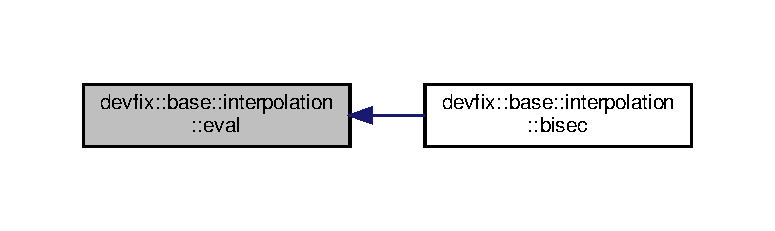
\includegraphics[width=350pt]{structdevfix_1_1base_1_1interpolation_ab769ce14a1e3bb758fa7b8b8db812101_icgraph}
\end{center}
\end{figure}
\mbox{\Hypertarget{structdevfix_1_1base_1_1interpolation_a327edb7c780e1020721e3f45b4760f44}\label{structdevfix_1_1base_1_1interpolation_a327edb7c780e1020721e3f45b4760f44}} 
\index{devfix\+::base\+::interpolation@{devfix\+::base\+::interpolation}!eval@{eval}}
\index{eval@{eval}!devfix\+::base\+::interpolation@{devfix\+::base\+::interpolation}}
\subsubsection{\texorpdfstring{eval()}{eval()}\hspace{0.1cm}{\footnotesize\ttfamily [2/2]}}
{\footnotesize\ttfamily template$<$typename FloatT$>$ \\
static FloatT \hyperlink{structdevfix_1_1base_1_1interpolation}{devfix\+::base\+::interpolation}$<$ FloatT $>$\+::eval (\begin{DoxyParamCaption}\item[{const std\+::vector$<$ FloatT $>$ \&}]{xs,  }\item[{const std\+::vector$<$ FloatT $>$ \&}]{coeffs,  }\item[{FloatT}]{x }\end{DoxyParamCaption})\hspace{0.3cm}{\ttfamily [inline]}, {\ttfamily [static]}}



evaluates the polynomial by an argument 


\begin{DoxyParams}{Parameters}
{\em xs} & x values of interpolation \\
\hline
{\em coeffs} & of interpolation \\
\hline
{\em x} & argument for evaluation \\
\hline
\end{DoxyParams}
\begin{DoxyReturn}{Returns}
value of polynomial at x 
\end{DoxyReturn}


The documentation for this struct was generated from the following file\+:\begin{DoxyCompactItemize}
\item 
devfix/base/\hyperlink{interpolation_8h}{interpolation.\+h}\end{DoxyCompactItemize}

\hypertarget{structdevfix_1_1base_1_1error_1_1interruptedexception}{}\section{devfix\+:\+:base\+:\+:error\+:\+:interruptedexception Struct Reference}
\label{structdevfix_1_1base_1_1error_1_1interruptedexception}\index{devfix\+::base\+::error\+::interruptedexception@{devfix\+::base\+::error\+::interruptedexception}}


Thrown when an operation is interrupted, either before or during the activity.  




{\ttfamily \#include $<$interruptedexception.\+h$>$}



Inheritance diagram for devfix\+:\+:base\+:\+:error\+:\+:interruptedexception\+:
% FIG 0


Collaboration diagram for devfix\+:\+:base\+:\+:error\+:\+:interruptedexception\+:
% FIG 1
\subsection*{Public Member Functions}
\begin{DoxyCompactItemize}
\item 
\hyperlink{structdevfix_1_1base_1_1error_1_1interruptedexception_a9b2d1244ef3e3029d231be8b84fa4c16}{interruptedexception} (const std\+::string \&what\+\_\+arg, int err=-\/1)
\item 
\hyperlink{structdevfix_1_1base_1_1error_1_1interruptedexception_a244a67233ab2b7be511706d8398ed860}{interruptedexception} (const char $\ast$what\+\_\+arg, int err=-\/1)
\end{DoxyCompactItemize}
\subsection*{Additional Inherited Members}


\subsection{Detailed Description}
Thrown when an operation is interrupted, either before or during the activity. 

Occasionally a method may wish to test whether the current operation has been interrupted, and if so, to immediately throw this error. 

\subsection{Constructor \& Destructor Documentation}
\mbox{\Hypertarget{structdevfix_1_1base_1_1error_1_1interruptedexception_a9b2d1244ef3e3029d231be8b84fa4c16}\label{structdevfix_1_1base_1_1error_1_1interruptedexception_a9b2d1244ef3e3029d231be8b84fa4c16}} 
\index{devfix\+::base\+::error\+::interruptedexception@{devfix\+::base\+::error\+::interruptedexception}!interruptedexception@{interruptedexception}}
\index{interruptedexception@{interruptedexception}!devfix\+::base\+::error\+::interruptedexception@{devfix\+::base\+::error\+::interruptedexception}}
\subsubsection{\texorpdfstring{interruptedexception()}{interruptedexception()}\hspace{0.1cm}{\footnotesize\ttfamily [1/2]}}
{\footnotesize\ttfamily devfix\+::base\+::error\+::interruptedexception\+::interruptedexception (\begin{DoxyParamCaption}\item[{const std\+::string \&}]{what\+\_\+arg,  }\item[{int}]{err = {\ttfamily -\/1} }\end{DoxyParamCaption})\hspace{0.3cm}{\ttfamily [inline]}, {\ttfamily [explicit]}}

Constructs the error object with what\+\_\+arg as explanatory string that can be accessed through \hyperlink{structdevfix_1_1base_1_1error_1_1baseexception_a16327152a55d65b1e537825231fbd452}{what()}. 
\begin{DoxyParams}{Parameters}
{\em what\+\_\+arg} & explanatory std\+::string \\
\hline
{\em err} & c error code (errno) \\
\hline
\end{DoxyParams}
\mbox{\Hypertarget{structdevfix_1_1base_1_1error_1_1interruptedexception_a244a67233ab2b7be511706d8398ed860}\label{structdevfix_1_1base_1_1error_1_1interruptedexception_a244a67233ab2b7be511706d8398ed860}} 
\index{devfix\+::base\+::error\+::interruptedexception@{devfix\+::base\+::error\+::interruptedexception}!interruptedexception@{interruptedexception}}
\index{interruptedexception@{interruptedexception}!devfix\+::base\+::error\+::interruptedexception@{devfix\+::base\+::error\+::interruptedexception}}
\subsubsection{\texorpdfstring{interruptedexception()}{interruptedexception()}\hspace{0.1cm}{\footnotesize\ttfamily [2/2]}}
{\footnotesize\ttfamily devfix\+::base\+::error\+::interruptedexception\+::interruptedexception (\begin{DoxyParamCaption}\item[{const char $\ast$}]{what\+\_\+arg,  }\item[{int}]{err = {\ttfamily -\/1} }\end{DoxyParamCaption})\hspace{0.3cm}{\ttfamily [inline]}, {\ttfamily [explicit]}}

Constructs the error object with what\+\_\+arg as explanatory string that can be accessed through \hyperlink{structdevfix_1_1base_1_1error_1_1baseexception_a16327152a55d65b1e537825231fbd452}{what()}. 
\begin{DoxyParams}{Parameters}
{\em what\+\_\+arg} & explanatory c-\/string \\
\hline
{\em err} & c error code (errno) \\
\hline
\end{DoxyParams}


The documentation for this struct was generated from the following file\+:\begin{DoxyCompactItemize}
\item 
devfix/base/error/interruptedexception.\+h\end{DoxyCompactItemize}

\hypertarget{structdevfix_1_1base_1_1error_1_1ioexception}{}\section{devfix\+:\+:base\+:\+:error\+:\+:ioexception Struct Reference}
\label{structdevfix_1_1base_1_1error_1_1ioexception}\index{devfix\+::base\+::error\+::ioexception@{devfix\+::base\+::error\+::ioexception}}


Signals that an I/O error of some sort has occurred.  




{\ttfamily \#include $<$ioexception.\+h$>$}



Inheritance diagram for devfix\+:\+:base\+:\+:error\+:\+:ioexception\+:
% FIG 0


Collaboration diagram for devfix\+:\+:base\+:\+:error\+:\+:ioexception\+:
% FIG 1
\subsection*{Public Member Functions}
\begin{DoxyCompactItemize}
\item 
\hyperlink{structdevfix_1_1base_1_1error_1_1ioexception_acaf6aa89dc63021cbf6241b897c570da}{ioexception} (const std\+::string \&what\+\_\+arg, int err=-\/1)
\item 
\hyperlink{structdevfix_1_1base_1_1error_1_1ioexception_a93e7dfc50605b9f6a9c5cd78dac59a44}{ioexception} (const char $\ast$what\+\_\+arg, int err=-\/1)
\end{DoxyCompactItemize}
\subsection*{Additional Inherited Members}


\subsection{Detailed Description}
Signals that an I/O error of some sort has occurred. 

This class is the general class of exceptions produced by failed or interrupted I/O operations. 

\subsection{Constructor \& Destructor Documentation}
\mbox{\Hypertarget{structdevfix_1_1base_1_1error_1_1ioexception_acaf6aa89dc63021cbf6241b897c570da}\label{structdevfix_1_1base_1_1error_1_1ioexception_acaf6aa89dc63021cbf6241b897c570da}} 
\index{devfix\+::base\+::error\+::ioexception@{devfix\+::base\+::error\+::ioexception}!ioexception@{ioexception}}
\index{ioexception@{ioexception}!devfix\+::base\+::error\+::ioexception@{devfix\+::base\+::error\+::ioexception}}
\subsubsection{\texorpdfstring{ioexception()}{ioexception()}\hspace{0.1cm}{\footnotesize\ttfamily [1/2]}}
{\footnotesize\ttfamily devfix\+::base\+::error\+::ioexception\+::ioexception (\begin{DoxyParamCaption}\item[{const std\+::string \&}]{what\+\_\+arg,  }\item[{int}]{err = {\ttfamily -\/1} }\end{DoxyParamCaption})\hspace{0.3cm}{\ttfamily [inline]}, {\ttfamily [explicit]}}

Constructs the error object with what\+\_\+arg as explanatory string that can be accessed through \hyperlink{structdevfix_1_1base_1_1error_1_1baseexception_a16327152a55d65b1e537825231fbd452}{what()}. 
\begin{DoxyParams}{Parameters}
{\em what\+\_\+arg} & explanatory std\+::string \\
\hline
{\em err} & c error code (errno) \\
\hline
\end{DoxyParams}
\mbox{\Hypertarget{structdevfix_1_1base_1_1error_1_1ioexception_a93e7dfc50605b9f6a9c5cd78dac59a44}\label{structdevfix_1_1base_1_1error_1_1ioexception_a93e7dfc50605b9f6a9c5cd78dac59a44}} 
\index{devfix\+::base\+::error\+::ioexception@{devfix\+::base\+::error\+::ioexception}!ioexception@{ioexception}}
\index{ioexception@{ioexception}!devfix\+::base\+::error\+::ioexception@{devfix\+::base\+::error\+::ioexception}}
\subsubsection{\texorpdfstring{ioexception()}{ioexception()}\hspace{0.1cm}{\footnotesize\ttfamily [2/2]}}
{\footnotesize\ttfamily devfix\+::base\+::error\+::ioexception\+::ioexception (\begin{DoxyParamCaption}\item[{const char $\ast$}]{what\+\_\+arg,  }\item[{int}]{err = {\ttfamily -\/1} }\end{DoxyParamCaption})\hspace{0.3cm}{\ttfamily [inline]}, {\ttfamily [explicit]}}

Constructs the error object with what\+\_\+arg as explanatory string that can be accessed through \hyperlink{structdevfix_1_1base_1_1error_1_1baseexception_a16327152a55d65b1e537825231fbd452}{what()}. 
\begin{DoxyParams}{Parameters}
{\em what\+\_\+arg} & explanatory c-\/string \\
\hline
{\em err} & c error code (errno) \\
\hline
\end{DoxyParams}


The documentation for this struct was generated from the following file\+:\begin{DoxyCompactItemize}
\item 
devfix/base/error/ioexception.\+h\end{DoxyCompactItemize}

\hypertarget{structdevfix_1_1base_1_1math}{}\section{devfix\+:\+:base\+:\+:math Struct Reference}
\label{structdevfix_1_1base_1_1math}\index{devfix\+::base\+::math@{devfix\+::base\+::math}}


{\ttfamily \#include $<$math.\+h$>$}

\subsection*{Public Types}
\begin{DoxyCompactItemize}
\item 
{\footnotesize template$<$typename T , std\+::size\+\_\+t N, typename G , typename ... Args$>$ }\\using \hyperlink{structdevfix_1_1base_1_1math_a6f2114ac2cf825b518cf5fefa00af6e3}{Table} = \hyperlink{structdevfix_1_1base_1_1__math_1_1Table}{\+\_\+math\+::\+Table}$<$ T, N, G, Args... $>$
\end{DoxyCompactItemize}
\subsection*{Static Public Member Functions}
\begin{DoxyCompactItemize}
\item 
{\footnotesize template$<$class UnsignedT $>$ }\\static constexpr std\+::size\+\_\+t \hyperlink{structdevfix_1_1base_1_1math_ab1781c7edecc9c462f16335f534b2470}{countl\+\_\+zero} (UnsignedT x) noexcept
\item 
{\footnotesize template$<$typename UnsignedT $>$ }\\static constexpr std\+::size\+\_\+t \hyperlink{structdevfix_1_1base_1_1math_a3ea732698f7ebf65df433de95721a6c1}{floor\+Log2} (UnsignedT v)
\item 
{\footnotesize template$<$typename UnsignedT $>$ }\\static constexpr std\+::size\+\_\+t \hyperlink{structdevfix_1_1base_1_1math_a4aa317a84af4eb10be4474c90cb47afe}{exp2} (UnsignedT v)
\item 
{\footnotesize template$<$typename FloatT $>$ }\\static void \hyperlink{structdevfix_1_1base_1_1math_a212f0b2e675de08688438e5bafb450c7}{to\+\_\+complex} (const FloatT $\ast$field, std\+::size\+\_\+t len, std\+::complex$<$ FloatT $>$ $\ast$cfield)
\item 
{\footnotesize template$<$typename FloatT $>$ }\\static std\+::vector$<$ std\+::complex$<$ FloatT $>$ $>$ \hyperlink{structdevfix_1_1base_1_1math_ace2cb831db8aeccad7108bc411612544}{to\+\_\+complex} (const std\+::vector$<$ FloatT $>$ \&vec, std\+::size\+\_\+t len=0)
\item 
{\footnotesize template$<$typename FloatT , std\+::size\+\_\+t N, std\+::size\+\_\+t Len = 0$>$ }\\static std\+::array$<$ std\+::complex$<$ FloatT $>$, N $>$ \hyperlink{structdevfix_1_1base_1_1math_aa125625a1d4063dc4bd4de82f7367f14}{to\+\_\+complex} (const std\+::array$<$ FloatT, N $>$ \&arr)
\item 
static constexpr std\+::uint32\+\_\+t \hyperlink{structdevfix_1_1base_1_1math_af3260ac1a62b3e9f6feb0f212aa8f796}{reverse\+\_\+bits} (std\+::uint32\+\_\+t val, std\+::size\+\_\+t bits)
\item 
{\footnotesize template$<$typename UnsignedT $>$ }\\static constexpr UnsignedT \hyperlink{structdevfix_1_1base_1_1math_ac3c5661a2ec82e7ae00e899c2a3d2049}{popcount} (UnsignedT val)
\end{DoxyCompactItemize}


\subsection{Member Typedef Documentation}
\mbox{\Hypertarget{structdevfix_1_1base_1_1math_a6f2114ac2cf825b518cf5fefa00af6e3}\label{structdevfix_1_1base_1_1math_a6f2114ac2cf825b518cf5fefa00af6e3}} 
\index{devfix\+::base\+::math@{devfix\+::base\+::math}!Table@{Table}}
\index{Table@{Table}!devfix\+::base\+::math@{devfix\+::base\+::math}}
\subsubsection{\texorpdfstring{Table}{Table}}
{\footnotesize\ttfamily template$<$typename T , std\+::size\+\_\+t N, typename G , typename ... Args$>$ \\
using \hyperlink{structdevfix_1_1base_1_1math_a6f2114ac2cf825b518cf5fefa00af6e3}{devfix\+::base\+::math\+::\+Table} =  \hyperlink{structdevfix_1_1base_1_1__math_1_1Table}{\+\_\+math\+::\+Table}$<$T, N, G, Args...$>$}



\subsection{Member Function Documentation}
\mbox{\Hypertarget{structdevfix_1_1base_1_1math_ab1781c7edecc9c462f16335f534b2470}\label{structdevfix_1_1base_1_1math_ab1781c7edecc9c462f16335f534b2470}} 
\index{devfix\+::base\+::math@{devfix\+::base\+::math}!countl\+\_\+zero@{countl\+\_\+zero}}
\index{countl\+\_\+zero@{countl\+\_\+zero}!devfix\+::base\+::math@{devfix\+::base\+::math}}
\subsubsection{\texorpdfstring{countl\+\_\+zero()}{countl\_zero()}}
{\footnotesize\ttfamily template$<$class UnsignedT $>$ \\
static constexpr std\+::size\+\_\+t devfix\+::base\+::math\+::countl\+\_\+zero (\begin{DoxyParamCaption}\item[{UnsignedT}]{x }\end{DoxyParamCaption})\hspace{0.3cm}{\ttfamily [inline]}, {\ttfamily [static]}, {\ttfamily [noexcept]}}

\mbox{\Hypertarget{structdevfix_1_1base_1_1math_a4aa317a84af4eb10be4474c90cb47afe}\label{structdevfix_1_1base_1_1math_a4aa317a84af4eb10be4474c90cb47afe}} 
\index{devfix\+::base\+::math@{devfix\+::base\+::math}!exp2@{exp2}}
\index{exp2@{exp2}!devfix\+::base\+::math@{devfix\+::base\+::math}}
\subsubsection{\texorpdfstring{exp2()}{exp2()}}
{\footnotesize\ttfamily template$<$typename UnsignedT $>$ \\
static constexpr std\+::size\+\_\+t devfix\+::base\+::math\+::exp2 (\begin{DoxyParamCaption}\item[{UnsignedT}]{v }\end{DoxyParamCaption})\hspace{0.3cm}{\ttfamily [inline]}, {\ttfamily [static]}}

Here is the caller graph for this function\+:
\nopagebreak
\begin{figure}[H]
\begin{center}
\leavevmode
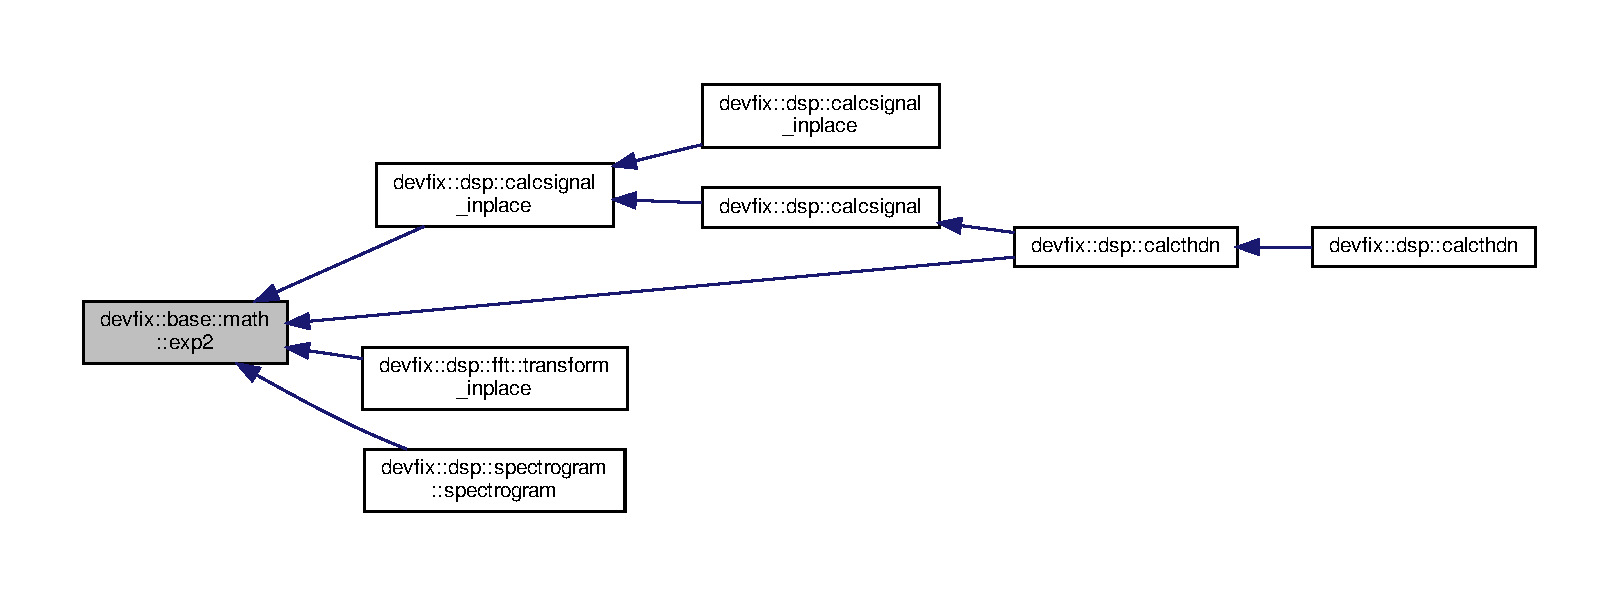
\includegraphics[width=350pt]{structdevfix_1_1base_1_1math_a4aa317a84af4eb10be4474c90cb47afe_icgraph}
\end{center}
\end{figure}
\mbox{\Hypertarget{structdevfix_1_1base_1_1math_a3ea732698f7ebf65df433de95721a6c1}\label{structdevfix_1_1base_1_1math_a3ea732698f7ebf65df433de95721a6c1}} 
\index{devfix\+::base\+::math@{devfix\+::base\+::math}!floor\+Log2@{floor\+Log2}}
\index{floor\+Log2@{floor\+Log2}!devfix\+::base\+::math@{devfix\+::base\+::math}}
\subsubsection{\texorpdfstring{floor\+Log2()}{floorLog2()}}
{\footnotesize\ttfamily template$<$typename UnsignedT $>$ \\
static constexpr std\+::size\+\_\+t devfix\+::base\+::math\+::floor\+Log2 (\begin{DoxyParamCaption}\item[{UnsignedT}]{v }\end{DoxyParamCaption})\hspace{0.3cm}{\ttfamily [inline]}, {\ttfamily [static]}}

Here is the caller graph for this function\+:
\nopagebreak
\begin{figure}[H]
\begin{center}
\leavevmode
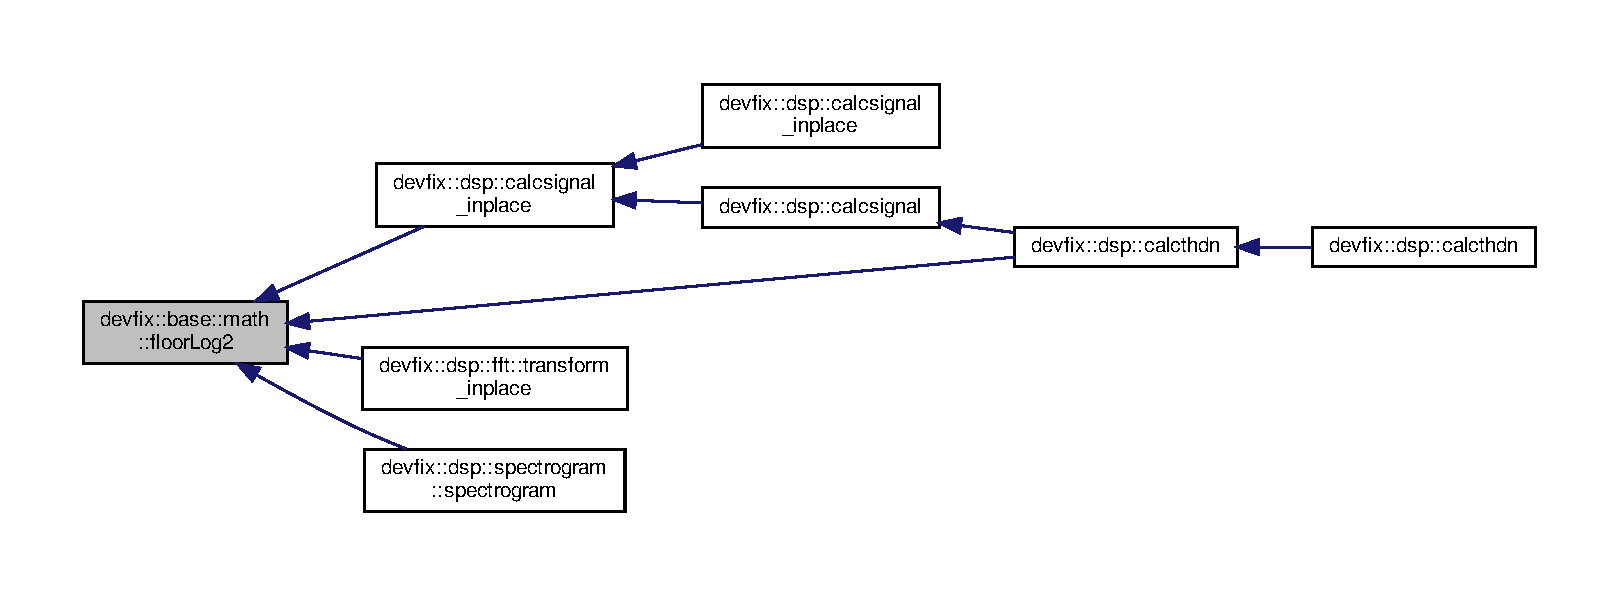
\includegraphics[width=350pt]{structdevfix_1_1base_1_1math_a3ea732698f7ebf65df433de95721a6c1_icgraph}
\end{center}
\end{figure}
\mbox{\Hypertarget{structdevfix_1_1base_1_1math_ac3c5661a2ec82e7ae00e899c2a3d2049}\label{structdevfix_1_1base_1_1math_ac3c5661a2ec82e7ae00e899c2a3d2049}} 
\index{devfix\+::base\+::math@{devfix\+::base\+::math}!popcount@{popcount}}
\index{popcount@{popcount}!devfix\+::base\+::math@{devfix\+::base\+::math}}
\subsubsection{\texorpdfstring{popcount()}{popcount()}}
{\footnotesize\ttfamily template$<$typename UnsignedT $>$ \\
static constexpr UnsignedT devfix\+::base\+::math\+::popcount (\begin{DoxyParamCaption}\item[{UnsignedT}]{val }\end{DoxyParamCaption})\hspace{0.3cm}{\ttfamily [inline]}, {\ttfamily [static]}}

Here is the caller graph for this function\+:
\nopagebreak
\begin{figure}[H]
\begin{center}
\leavevmode
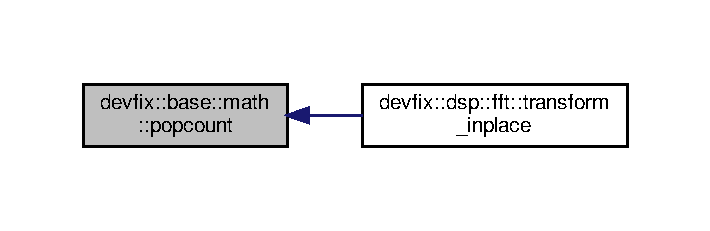
\includegraphics[width=341pt]{structdevfix_1_1base_1_1math_ac3c5661a2ec82e7ae00e899c2a3d2049_icgraph}
\end{center}
\end{figure}
\mbox{\Hypertarget{structdevfix_1_1base_1_1math_af3260ac1a62b3e9f6feb0f212aa8f796}\label{structdevfix_1_1base_1_1math_af3260ac1a62b3e9f6feb0f212aa8f796}} 
\index{devfix\+::base\+::math@{devfix\+::base\+::math}!reverse\+\_\+bits@{reverse\+\_\+bits}}
\index{reverse\+\_\+bits@{reverse\+\_\+bits}!devfix\+::base\+::math@{devfix\+::base\+::math}}
\subsubsection{\texorpdfstring{reverse\+\_\+bits()}{reverse\_bits()}}
{\footnotesize\ttfamily static constexpr std\+::uint32\+\_\+t devfix\+::base\+::math\+::reverse\+\_\+bits (\begin{DoxyParamCaption}\item[{std\+::uint32\+\_\+t}]{val,  }\item[{std\+::size\+\_\+t}]{bits }\end{DoxyParamCaption})\hspace{0.3cm}{\ttfamily [inline]}, {\ttfamily [static]}}

Here is the caller graph for this function\+:
\nopagebreak
\begin{figure}[H]
\begin{center}
\leavevmode
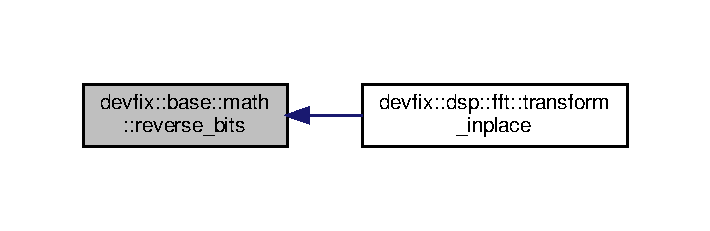
\includegraphics[width=341pt]{structdevfix_1_1base_1_1math_af3260ac1a62b3e9f6feb0f212aa8f796_icgraph}
\end{center}
\end{figure}
\mbox{\Hypertarget{structdevfix_1_1base_1_1math_a212f0b2e675de08688438e5bafb450c7}\label{structdevfix_1_1base_1_1math_a212f0b2e675de08688438e5bafb450c7}} 
\index{devfix\+::base\+::math@{devfix\+::base\+::math}!to\+\_\+complex@{to\+\_\+complex}}
\index{to\+\_\+complex@{to\+\_\+complex}!devfix\+::base\+::math@{devfix\+::base\+::math}}
\subsubsection{\texorpdfstring{to\+\_\+complex()}{to\_complex()}\hspace{0.1cm}{\footnotesize\ttfamily [1/3]}}
{\footnotesize\ttfamily template$<$typename FloatT $>$ \\
static void devfix\+::base\+::math\+::to\+\_\+complex (\begin{DoxyParamCaption}\item[{const FloatT $\ast$}]{field,  }\item[{std\+::size\+\_\+t}]{len,  }\item[{std\+::complex$<$ FloatT $>$ $\ast$}]{cfield }\end{DoxyParamCaption})\hspace{0.3cm}{\ttfamily [inline]}, {\ttfamily [static]}}

Here is the caller graph for this function\+:
\nopagebreak
\begin{figure}[H]
\begin{center}
\leavevmode
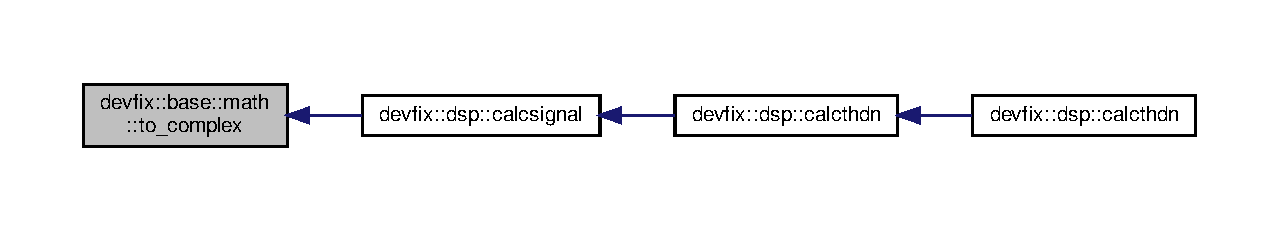
\includegraphics[width=350pt]{structdevfix_1_1base_1_1math_a212f0b2e675de08688438e5bafb450c7_icgraph}
\end{center}
\end{figure}
\mbox{\Hypertarget{structdevfix_1_1base_1_1math_ace2cb831db8aeccad7108bc411612544}\label{structdevfix_1_1base_1_1math_ace2cb831db8aeccad7108bc411612544}} 
\index{devfix\+::base\+::math@{devfix\+::base\+::math}!to\+\_\+complex@{to\+\_\+complex}}
\index{to\+\_\+complex@{to\+\_\+complex}!devfix\+::base\+::math@{devfix\+::base\+::math}}
\subsubsection{\texorpdfstring{to\+\_\+complex()}{to\_complex()}\hspace{0.1cm}{\footnotesize\ttfamily [2/3]}}
{\footnotesize\ttfamily template$<$typename FloatT $>$ \\
static std\+::vector$<$std\+::complex$<$FloatT$>$ $>$ devfix\+::base\+::math\+::to\+\_\+complex (\begin{DoxyParamCaption}\item[{const std\+::vector$<$ FloatT $>$ \&}]{vec,  }\item[{std\+::size\+\_\+t}]{len = {\ttfamily 0} }\end{DoxyParamCaption})\hspace{0.3cm}{\ttfamily [inline]}, {\ttfamily [static]}}

\mbox{\Hypertarget{structdevfix_1_1base_1_1math_aa125625a1d4063dc4bd4de82f7367f14}\label{structdevfix_1_1base_1_1math_aa125625a1d4063dc4bd4de82f7367f14}} 
\index{devfix\+::base\+::math@{devfix\+::base\+::math}!to\+\_\+complex@{to\+\_\+complex}}
\index{to\+\_\+complex@{to\+\_\+complex}!devfix\+::base\+::math@{devfix\+::base\+::math}}
\subsubsection{\texorpdfstring{to\+\_\+complex()}{to\_complex()}\hspace{0.1cm}{\footnotesize\ttfamily [3/3]}}
{\footnotesize\ttfamily template$<$typename FloatT , std\+::size\+\_\+t N, std\+::size\+\_\+t Len = 0$>$ \\
static std\+::array$<$std\+::complex$<$FloatT$>$, N$>$ devfix\+::base\+::math\+::to\+\_\+complex (\begin{DoxyParamCaption}\item[{const std\+::array$<$ FloatT, N $>$ \&}]{arr }\end{DoxyParamCaption})\hspace{0.3cm}{\ttfamily [inline]}, {\ttfamily [static]}}



The documentation for this struct was generated from the following file\+:\begin{DoxyCompactItemize}
\item 
devfix/base/\hyperlink{math_8h}{math.\+h}\end{DoxyCompactItemize}

\hypertarget{structdevfix_1_1net_1_1netbuilder}{}\section{devfix\+:\+:net\+:\+:netbuilder Struct Reference}
\label{structdevfix_1_1net_1_1netbuilder}\index{devfix\+::net\+::netbuilder@{devfix\+::net\+::netbuilder}}
\subsection*{Static Public Member Functions}
\begin{DoxyCompactItemize}
\item 
static std\+::unique\+\_\+ptr$<$ \hyperlink{structdevfix_1_1net_1_1socket}{socket} $>$ \hyperlink{structdevfix_1_1net_1_1netbuilder_a9d9eb6cb050ca920aa647baaf4692405}{create\+\_\+socket} (\hyperlink{structdevfix_1_1net_1_1inetaddress}{inetaddress} adr)
\begin{DoxyCompactList}\small\item\em Creates a socket and connects it to the specified remote internet address. The Socket will also bind() to the local address and port supplied. \end{DoxyCompactList}\item 
\mbox{\Hypertarget{structdevfix_1_1net_1_1netbuilder_a9d685e1822c0be5d68fd6ba62876798b}\label{structdevfix_1_1net_1_1netbuilder_a9d685e1822c0be5d68fd6ba62876798b}} 
static std\+::unique\+\_\+ptr$<$ \hyperlink{structdevfix_1_1net_1_1serversocket}{serversocket} $>$ {\bfseries create\+\_\+serversocket} (\hyperlink{structdevfix_1_1net_1_1inetaddress}{inetaddress} adr, bool reuse\+\_\+address=false)
\end{DoxyCompactItemize}


\subsection{Member Function Documentation}
\mbox{\Hypertarget{structdevfix_1_1net_1_1netbuilder_a9d9eb6cb050ca920aa647baaf4692405}\label{structdevfix_1_1net_1_1netbuilder_a9d9eb6cb050ca920aa647baaf4692405}} 
\index{devfix\+::net\+::netbuilder@{devfix\+::net\+::netbuilder}!create\+\_\+socket@{create\+\_\+socket}}
\index{create\+\_\+socket@{create\+\_\+socket}!devfix\+::net\+::netbuilder@{devfix\+::net\+::netbuilder}}
\subsubsection{\texorpdfstring{create\+\_\+socket()}{create\_socket()}}
{\footnotesize\ttfamily std\+::unique\+\_\+ptr$<$ \hyperlink{structdevfix_1_1net_1_1socket}{socket} $>$ devfix\+::net\+::netbuilder\+::create\+\_\+socket (\begin{DoxyParamCaption}\item[{\hyperlink{structdevfix_1_1net_1_1inetaddress}{inetaddress}}]{adr }\end{DoxyParamCaption})\hspace{0.3cm}{\ttfamily [static]}}



Creates a socket and connects it to the specified remote internet address. The Socket will also bind() to the local address and port supplied. 


\begin{DoxyParams}{Parameters}
{\em inetaddress} & remote address \\
\hline
\end{DoxyParams}
\begin{DoxyReturn}{Returns}

\end{DoxyReturn}


The documentation for this struct was generated from the following files\+:\begin{DoxyCompactItemize}
\item 
devfix/net/netbuilder.\+h\item 
devfix/net/netbuilder.\+cpp\end{DoxyCompactItemize}

\hypertarget{structdevfix_1_1base_1_1io_1_1outputstream}{}\section{devfix\+:\+:base\+:\+:io\+:\+:outputstream Struct Reference}
\label{structdevfix_1_1base_1_1io_1_1outputstream}\index{devfix\+::base\+::io\+::outputstream@{devfix\+::base\+::io\+::outputstream}}


Superclass of all classes representing an output stream of bytes.  




{\ttfamily \#include $<$outputstream.\+h$>$}



Inheritance diagram for devfix\+:\+:base\+:\+:io\+:\+:outputstream\+:\nopagebreak
\begin{figure}[H]
\begin{center}
\leavevmode
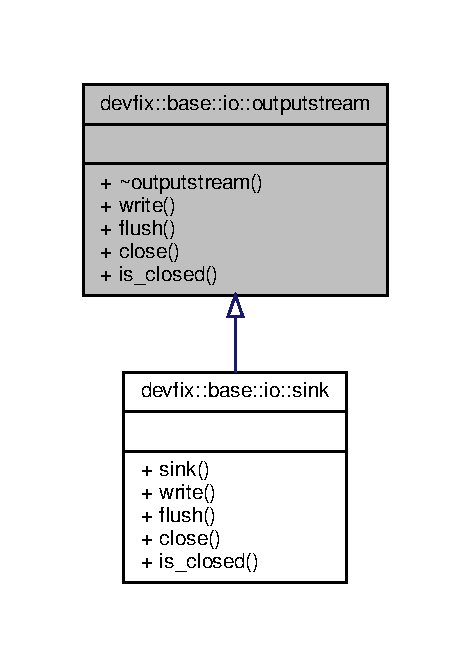
\includegraphics[width=226pt]{structdevfix_1_1base_1_1io_1_1outputstream__inherit__graph}
\end{center}
\end{figure}
\subsection*{Public Member Functions}
\begin{DoxyCompactItemize}
\item 
virtual \hyperlink{structdevfix_1_1base_1_1io_1_1outputstream_a9154a8859d44c7929c98fb83e03047e3}{$\sim$outputstream} ()=default
\item 
virtual void \hyperlink{structdevfix_1_1base_1_1io_1_1outputstream_ac7e5fcd6883c7c8f53356a4eb8284c00}{write} (const void $\ast$buf, std\+::size\+\_\+t len)=0
\begin{DoxyCompactList}\small\item\em Writes len bytes from the specified buffer to this output stream. \end{DoxyCompactList}\item 
virtual void \hyperlink{structdevfix_1_1base_1_1io_1_1outputstream_a3fe3b34675a2d70331e6ca235388e0cc}{flush} ()=0
\begin{DoxyCompactList}\small\item\em Flushes this {\itshape outputstream} and forces any buffered output bytes to be written out. \end{DoxyCompactList}\item 
virtual void \hyperlink{structdevfix_1_1base_1_1io_1_1outputstream_a060c2e7040e6bb831b8150f64bd8abf7}{close} ()=0
\begin{DoxyCompactList}\small\item\em Closes this {\itshape outputstream} and releases any system resources associated with this stream. \end{DoxyCompactList}\item 
virtual bool \hyperlink{structdevfix_1_1base_1_1io_1_1outputstream_a52bd2eac8f6fbc496eab5138a48d2f06}{is\+\_\+closed} ()=0
\begin{DoxyCompactList}\small\item\em Returns if the {\itshape outputstream} is closed or available for further calls of output operations. \end{DoxyCompactList}\end{DoxyCompactItemize}


\subsection{Detailed Description}
Superclass of all classes representing an output stream of bytes. 

An output stream accepts output bytes and sends them to some sink. Applications that need to define a subclass of Output\+Stream must always provide a method that writes one byte of output. 

\subsection{Constructor \& Destructor Documentation}
\mbox{\Hypertarget{structdevfix_1_1base_1_1io_1_1outputstream_a9154a8859d44c7929c98fb83e03047e3}\label{structdevfix_1_1base_1_1io_1_1outputstream_a9154a8859d44c7929c98fb83e03047e3}} 
\index{devfix\+::base\+::io\+::outputstream@{devfix\+::base\+::io\+::outputstream}!````~outputstream@{$\sim$outputstream}}
\index{````~outputstream@{$\sim$outputstream}!devfix\+::base\+::io\+::outputstream@{devfix\+::base\+::io\+::outputstream}}
\subsubsection{\texorpdfstring{$\sim$outputstream()}{~outputstream()}}
{\footnotesize\ttfamily virtual devfix\+::base\+::io\+::outputstream\+::$\sim$outputstream (\begin{DoxyParamCaption}{ }\end{DoxyParamCaption})\hspace{0.3cm}{\ttfamily [virtual]}, {\ttfamily [default]}}



\subsection{Member Function Documentation}
\mbox{\Hypertarget{structdevfix_1_1base_1_1io_1_1outputstream_a060c2e7040e6bb831b8150f64bd8abf7}\label{structdevfix_1_1base_1_1io_1_1outputstream_a060c2e7040e6bb831b8150f64bd8abf7}} 
\index{devfix\+::base\+::io\+::outputstream@{devfix\+::base\+::io\+::outputstream}!close@{close}}
\index{close@{close}!devfix\+::base\+::io\+::outputstream@{devfix\+::base\+::io\+::outputstream}}
\subsubsection{\texorpdfstring{close()}{close()}}
{\footnotesize\ttfamily virtual void devfix\+::base\+::io\+::outputstream\+::close (\begin{DoxyParamCaption}{ }\end{DoxyParamCaption})\hspace{0.3cm}{\ttfamily [pure virtual]}}



Closes this {\itshape outputstream} and releases any system resources associated with this stream. 

The general contract of close is that it closes the output stream. A closed stream cannot perform output operations and cannot be reopened. 

Implemented in \hyperlink{structdevfix_1_1base_1_1io_1_1sink_a2d110d27baa88f462540e7fd59fb8b3c}{devfix\+::base\+::io\+::sink}.

\mbox{\Hypertarget{structdevfix_1_1base_1_1io_1_1outputstream_a3fe3b34675a2d70331e6ca235388e0cc}\label{structdevfix_1_1base_1_1io_1_1outputstream_a3fe3b34675a2d70331e6ca235388e0cc}} 
\index{devfix\+::base\+::io\+::outputstream@{devfix\+::base\+::io\+::outputstream}!flush@{flush}}
\index{flush@{flush}!devfix\+::base\+::io\+::outputstream@{devfix\+::base\+::io\+::outputstream}}
\subsubsection{\texorpdfstring{flush()}{flush()}}
{\footnotesize\ttfamily virtual void devfix\+::base\+::io\+::outputstream\+::flush (\begin{DoxyParamCaption}{ }\end{DoxyParamCaption})\hspace{0.3cm}{\ttfamily [pure virtual]}}



Flushes this {\itshape outputstream} and forces any buffered output bytes to be written out. 

The general contract of flush is that calling it is an indication that, if any bytes previously written have been buffered by the implementation of the output stream, such bytes should immediately be written to their intended destination.

If the intended destination of this stream is an abstraction provided by the underlying operating system, for example a file, then flushing the stream guarantees only that bytes previously written to the stream are passed to the operating system for writing; it does not guarantee that they are actually written to a physical device such as a disk drive. 

Implemented in \hyperlink{structdevfix_1_1base_1_1io_1_1sink_abf208747c9be8295972fbc4696ddc557}{devfix\+::base\+::io\+::sink}.

\mbox{\Hypertarget{structdevfix_1_1base_1_1io_1_1outputstream_a52bd2eac8f6fbc496eab5138a48d2f06}\label{structdevfix_1_1base_1_1io_1_1outputstream_a52bd2eac8f6fbc496eab5138a48d2f06}} 
\index{devfix\+::base\+::io\+::outputstream@{devfix\+::base\+::io\+::outputstream}!is\+\_\+closed@{is\+\_\+closed}}
\index{is\+\_\+closed@{is\+\_\+closed}!devfix\+::base\+::io\+::outputstream@{devfix\+::base\+::io\+::outputstream}}
\subsubsection{\texorpdfstring{is\+\_\+closed()}{is\_closed()}}
{\footnotesize\ttfamily virtual bool devfix\+::base\+::io\+::outputstream\+::is\+\_\+closed (\begin{DoxyParamCaption}{ }\end{DoxyParamCaption})\hspace{0.3cm}{\ttfamily [pure virtual]}}



Returns if the {\itshape outputstream} is closed or available for further calls of output operations. 

\begin{DoxyReturn}{Returns}
true if the {\itshape outputstream} got previously closed. 
\end{DoxyReturn}


Implemented in \hyperlink{structdevfix_1_1base_1_1io_1_1sink_a1e5782219f9256d8ff09385fa6f3b156}{devfix\+::base\+::io\+::sink}.

\mbox{\Hypertarget{structdevfix_1_1base_1_1io_1_1outputstream_ac7e5fcd6883c7c8f53356a4eb8284c00}\label{structdevfix_1_1base_1_1io_1_1outputstream_ac7e5fcd6883c7c8f53356a4eb8284c00}} 
\index{devfix\+::base\+::io\+::outputstream@{devfix\+::base\+::io\+::outputstream}!write@{write}}
\index{write@{write}!devfix\+::base\+::io\+::outputstream@{devfix\+::base\+::io\+::outputstream}}
\subsubsection{\texorpdfstring{write()}{write()}}
{\footnotesize\ttfamily virtual void devfix\+::base\+::io\+::outputstream\+::write (\begin{DoxyParamCaption}\item[{const void $\ast$}]{buf,  }\item[{std\+::size\+\_\+t}]{len }\end{DoxyParamCaption})\hspace{0.3cm}{\ttfamily [pure virtual]}}



Writes len bytes from the specified buffer to this output stream. 

Element b\mbox{[}0\mbox{]} is the first byte written and b\mbox{[}len-\/1\mbox{]} is the last byte written by this operation.


\begin{DoxyParams}{Parameters}
{\em buf} & the data. \\
\hline
{\em len} & the number of bytes to write. \\
\hline
\end{DoxyParams}


Implemented in \hyperlink{structdevfix_1_1base_1_1io_1_1sink_a6eade9933d316139e952b7a442f3c56d}{devfix\+::base\+::io\+::sink}.



The documentation for this struct was generated from the following file\+:\begin{DoxyCompactItemize}
\item 
devfix/base/io/\hyperlink{outputstream_8h}{outputstream.\+h}\end{DoxyCompactItemize}

\hypertarget{structdevfix_1_1base_1_1platform}{}\section{devfix\+:\+:base\+:\+:platform Struct Reference}
\label{structdevfix_1_1base_1_1platform}\index{devfix\+::base\+::platform@{devfix\+::base\+::platform}}


{\ttfamily \#include $<$platform.\+h$>$}

\subsection*{Static Public Member Functions}
\begin{DoxyCompactItemize}
\item 
static constexpr const char $\ast$ \hyperlink{structdevfix_1_1base_1_1platform_a5d491c9eadd0e09eafda6263852d37e4}{get\+\_\+filename} (const char $\ast$fname)
\end{DoxyCompactItemize}


\subsection{Member Function Documentation}
\mbox{\Hypertarget{structdevfix_1_1base_1_1platform_a5d491c9eadd0e09eafda6263852d37e4}\label{structdevfix_1_1base_1_1platform_a5d491c9eadd0e09eafda6263852d37e4}} 
\index{devfix\+::base\+::platform@{devfix\+::base\+::platform}!get\+\_\+filename@{get\+\_\+filename}}
\index{get\+\_\+filename@{get\+\_\+filename}!devfix\+::base\+::platform@{devfix\+::base\+::platform}}
\subsubsection{\texorpdfstring{get\+\_\+filename()}{get\_filename()}}
{\footnotesize\ttfamily static constexpr const char$\ast$ devfix\+::base\+::platform\+::get\+\_\+filename (\begin{DoxyParamCaption}\item[{const char $\ast$}]{fname }\end{DoxyParamCaption})\hspace{0.3cm}{\ttfamily [inline]}, {\ttfamily [static]}}



The documentation for this struct was generated from the following file\+:\begin{DoxyCompactItemize}
\item 
devfix/base/\hyperlink{platform_8h}{platform.\+h}\end{DoxyCompactItemize}

\hypertarget{structdevfix_1_1net_1_1serversocket}{}\section{devfix\+:\+:net\+:\+:serversocket Struct Reference}
\label{structdevfix_1_1net_1_1serversocket}\index{devfix\+::net\+::serversocket@{devfix\+::net\+::serversocket}}


{\ttfamily \#include $<$serversocket.\+h$>$}

\subsection*{Public Member Functions}
\begin{DoxyCompactItemize}
\item 
virtual \hyperlink{structdevfix_1_1net_1_1serversocket_afd9f315c4018808c790478710f52d8ab}{$\sim$serversocket} ()=default
\item 
virtual std\+::unique\+\_\+ptr$<$ \hyperlink{structdevfix_1_1net_1_1socket}{socket} $>$ \hyperlink{structdevfix_1_1net_1_1serversocket_a7b3ea6aad486060acdd1385a08f7db81}{accept} ()=0
\item 
virtual const \hyperlink{structdevfix_1_1net_1_1inetaddress}{inetaddress} \& \hyperlink{structdevfix_1_1net_1_1serversocket_a087a819b8173bfa101ea65ea8a17eb8c}{get\+\_\+address} () const noexcept=0
\item 
virtual bool \hyperlink{structdevfix_1_1net_1_1serversocket_a7efdb1f57d0e482542fda50a2403230d}{get\+\_\+reuse\+\_\+address} () const noexcept=0
\item 
virtual void \hyperlink{structdevfix_1_1net_1_1serversocket_ae67a25cf26fe54ce7b10d07ff9219ce7}{set\+\_\+accept\+\_\+timeout} (\hyperlink{structdevfix_1_1net_1_1socket_a80a3bf4cb7292bae31ea9c6575539c68}{socket\+::timeout\+\_\+t} timeout)=0
\item 
virtual \hyperlink{structdevfix_1_1net_1_1socket_a80a3bf4cb7292bae31ea9c6575539c68}{socket\+::timeout\+\_\+t} \hyperlink{structdevfix_1_1net_1_1serversocket_acde0979277bf9536f54bb0fb6a9cc881}{get\+\_\+accept\+\_\+timeout} () const noexcept=0
\item 
virtual void \hyperlink{structdevfix_1_1net_1_1serversocket_ab1762c3364c8298dbac6c3dd67a1e7aa}{close} ()=0
\item 
virtual bool \hyperlink{structdevfix_1_1net_1_1serversocket_a37cc4e3ecede2a0bc52f90e49fcbe4a9}{is\+\_\+closed} () const noexcept=0
\end{DoxyCompactItemize}


\subsection{Constructor \& Destructor Documentation}
\mbox{\Hypertarget{structdevfix_1_1net_1_1serversocket_afd9f315c4018808c790478710f52d8ab}\label{structdevfix_1_1net_1_1serversocket_afd9f315c4018808c790478710f52d8ab}} 
\index{devfix\+::net\+::serversocket@{devfix\+::net\+::serversocket}!````~serversocket@{$\sim$serversocket}}
\index{````~serversocket@{$\sim$serversocket}!devfix\+::net\+::serversocket@{devfix\+::net\+::serversocket}}
\subsubsection{\texorpdfstring{$\sim$serversocket()}{~serversocket()}}
{\footnotesize\ttfamily virtual devfix\+::net\+::serversocket\+::$\sim$serversocket (\begin{DoxyParamCaption}{ }\end{DoxyParamCaption})\hspace{0.3cm}{\ttfamily [virtual]}, {\ttfamily [default]}}



\subsection{Member Function Documentation}
\mbox{\Hypertarget{structdevfix_1_1net_1_1serversocket_a7b3ea6aad486060acdd1385a08f7db81}\label{structdevfix_1_1net_1_1serversocket_a7b3ea6aad486060acdd1385a08f7db81}} 
\index{devfix\+::net\+::serversocket@{devfix\+::net\+::serversocket}!accept@{accept}}
\index{accept@{accept}!devfix\+::net\+::serversocket@{devfix\+::net\+::serversocket}}
\subsubsection{\texorpdfstring{accept()}{accept()}}
{\footnotesize\ttfamily virtual std\+::unique\+\_\+ptr$<$\hyperlink{structdevfix_1_1net_1_1socket}{socket}$>$ devfix\+::net\+::serversocket\+::accept (\begin{DoxyParamCaption}{ }\end{DoxyParamCaption})\hspace{0.3cm}{\ttfamily [pure virtual]}}

\mbox{\Hypertarget{structdevfix_1_1net_1_1serversocket_ab1762c3364c8298dbac6c3dd67a1e7aa}\label{structdevfix_1_1net_1_1serversocket_ab1762c3364c8298dbac6c3dd67a1e7aa}} 
\index{devfix\+::net\+::serversocket@{devfix\+::net\+::serversocket}!close@{close}}
\index{close@{close}!devfix\+::net\+::serversocket@{devfix\+::net\+::serversocket}}
\subsubsection{\texorpdfstring{close()}{close()}}
{\footnotesize\ttfamily virtual void devfix\+::net\+::serversocket\+::close (\begin{DoxyParamCaption}{ }\end{DoxyParamCaption})\hspace{0.3cm}{\ttfamily [pure virtual]}}

\mbox{\Hypertarget{structdevfix_1_1net_1_1serversocket_acde0979277bf9536f54bb0fb6a9cc881}\label{structdevfix_1_1net_1_1serversocket_acde0979277bf9536f54bb0fb6a9cc881}} 
\index{devfix\+::net\+::serversocket@{devfix\+::net\+::serversocket}!get\+\_\+accept\+\_\+timeout@{get\+\_\+accept\+\_\+timeout}}
\index{get\+\_\+accept\+\_\+timeout@{get\+\_\+accept\+\_\+timeout}!devfix\+::net\+::serversocket@{devfix\+::net\+::serversocket}}
\subsubsection{\texorpdfstring{get\+\_\+accept\+\_\+timeout()}{get\_accept\_timeout()}}
{\footnotesize\ttfamily virtual \hyperlink{structdevfix_1_1net_1_1socket_a80a3bf4cb7292bae31ea9c6575539c68}{socket\+::timeout\+\_\+t} devfix\+::net\+::serversocket\+::get\+\_\+accept\+\_\+timeout (\begin{DoxyParamCaption}{ }\end{DoxyParamCaption}) const\hspace{0.3cm}{\ttfamily [pure virtual]}, {\ttfamily [noexcept]}}

\mbox{\Hypertarget{structdevfix_1_1net_1_1serversocket_a087a819b8173bfa101ea65ea8a17eb8c}\label{structdevfix_1_1net_1_1serversocket_a087a819b8173bfa101ea65ea8a17eb8c}} 
\index{devfix\+::net\+::serversocket@{devfix\+::net\+::serversocket}!get\+\_\+address@{get\+\_\+address}}
\index{get\+\_\+address@{get\+\_\+address}!devfix\+::net\+::serversocket@{devfix\+::net\+::serversocket}}
\subsubsection{\texorpdfstring{get\+\_\+address()}{get\_address()}}
{\footnotesize\ttfamily virtual const \hyperlink{structdevfix_1_1net_1_1inetaddress}{inetaddress}\& devfix\+::net\+::serversocket\+::get\+\_\+address (\begin{DoxyParamCaption}{ }\end{DoxyParamCaption}) const\hspace{0.3cm}{\ttfamily [pure virtual]}, {\ttfamily [noexcept]}}

\mbox{\Hypertarget{structdevfix_1_1net_1_1serversocket_a7efdb1f57d0e482542fda50a2403230d}\label{structdevfix_1_1net_1_1serversocket_a7efdb1f57d0e482542fda50a2403230d}} 
\index{devfix\+::net\+::serversocket@{devfix\+::net\+::serversocket}!get\+\_\+reuse\+\_\+address@{get\+\_\+reuse\+\_\+address}}
\index{get\+\_\+reuse\+\_\+address@{get\+\_\+reuse\+\_\+address}!devfix\+::net\+::serversocket@{devfix\+::net\+::serversocket}}
\subsubsection{\texorpdfstring{get\+\_\+reuse\+\_\+address()}{get\_reuse\_address()}}
{\footnotesize\ttfamily virtual bool devfix\+::net\+::serversocket\+::get\+\_\+reuse\+\_\+address (\begin{DoxyParamCaption}{ }\end{DoxyParamCaption}) const\hspace{0.3cm}{\ttfamily [pure virtual]}, {\ttfamily [noexcept]}}

\mbox{\Hypertarget{structdevfix_1_1net_1_1serversocket_a37cc4e3ecede2a0bc52f90e49fcbe4a9}\label{structdevfix_1_1net_1_1serversocket_a37cc4e3ecede2a0bc52f90e49fcbe4a9}} 
\index{devfix\+::net\+::serversocket@{devfix\+::net\+::serversocket}!is\+\_\+closed@{is\+\_\+closed}}
\index{is\+\_\+closed@{is\+\_\+closed}!devfix\+::net\+::serversocket@{devfix\+::net\+::serversocket}}
\subsubsection{\texorpdfstring{is\+\_\+closed()}{is\_closed()}}
{\footnotesize\ttfamily virtual bool devfix\+::net\+::serversocket\+::is\+\_\+closed (\begin{DoxyParamCaption}{ }\end{DoxyParamCaption}) const\hspace{0.3cm}{\ttfamily [pure virtual]}, {\ttfamily [noexcept]}}

\mbox{\Hypertarget{structdevfix_1_1net_1_1serversocket_ae67a25cf26fe54ce7b10d07ff9219ce7}\label{structdevfix_1_1net_1_1serversocket_ae67a25cf26fe54ce7b10d07ff9219ce7}} 
\index{devfix\+::net\+::serversocket@{devfix\+::net\+::serversocket}!set\+\_\+accept\+\_\+timeout@{set\+\_\+accept\+\_\+timeout}}
\index{set\+\_\+accept\+\_\+timeout@{set\+\_\+accept\+\_\+timeout}!devfix\+::net\+::serversocket@{devfix\+::net\+::serversocket}}
\subsubsection{\texorpdfstring{set\+\_\+accept\+\_\+timeout()}{set\_accept\_timeout()}}
{\footnotesize\ttfamily virtual void devfix\+::net\+::serversocket\+::set\+\_\+accept\+\_\+timeout (\begin{DoxyParamCaption}\item[{\hyperlink{structdevfix_1_1net_1_1socket_a80a3bf4cb7292bae31ea9c6575539c68}{socket\+::timeout\+\_\+t}}]{timeout }\end{DoxyParamCaption})\hspace{0.3cm}{\ttfamily [pure virtual]}}



The documentation for this struct was generated from the following file\+:\begin{DoxyCompactItemize}
\item 
devfix/net/\hyperlink{serversocket_8h}{serversocket.\+h}\end{DoxyCompactItemize}

\hypertarget{structdevfix_1_1base_1_1io_1_1sink}{}\section{devfix\+:\+:base\+:\+:io\+:\+:sink Struct Reference}
\label{structdevfix_1_1base_1_1io_1_1sink}\index{devfix\+::base\+::io\+::sink@{devfix\+::base\+::io\+::sink}}


Inheritance diagram for devfix\+:\+:base\+:\+:io\+:\+:sink\+:
% FIG 0


Collaboration diagram for devfix\+:\+:base\+:\+:io\+:\+:sink\+:
% FIG 1
\subsection*{Public Member Functions}
\begin{DoxyCompactItemize}
\item 
\mbox{\Hypertarget{structdevfix_1_1base_1_1io_1_1sink_a5e065482904521fde4ac8d0e378529c8}\label{structdevfix_1_1base_1_1io_1_1sink_a5e065482904521fde4ac8d0e378529c8}} 
{\bfseries sink} (write\+\_\+t write, flush\+\_\+t flush, close\+\_\+t close=D\+E\+F\+A\+U\+L\+T\+\_\+\+C\+L\+O\+SE, is\+\_\+closed\+\_\+t is\+\_\+closed=D\+E\+F\+A\+U\+L\+T\+\_\+\+I\+S\+\_\+\+C\+L\+O\+S\+ED)
\item 
\mbox{\Hypertarget{structdevfix_1_1base_1_1io_1_1sink_a912eebd869f230d506a2c8fcd69051b4}\label{structdevfix_1_1base_1_1io_1_1sink_a912eebd869f230d506a2c8fcd69051b4}} 
void {\bfseries write} (void $\ast$buf, std\+::size\+\_\+t len)
\item 
\mbox{\Hypertarget{structdevfix_1_1base_1_1io_1_1sink_abf208747c9be8295972fbc4696ddc557}\label{structdevfix_1_1base_1_1io_1_1sink_abf208747c9be8295972fbc4696ddc557}} 
void {\bfseries flush} ()
\item 
\mbox{\Hypertarget{structdevfix_1_1base_1_1io_1_1sink_a2d110d27baa88f462540e7fd59fb8b3c}\label{structdevfix_1_1base_1_1io_1_1sink_a2d110d27baa88f462540e7fd59fb8b3c}} 
void {\bfseries close} ()
\item 
\mbox{\Hypertarget{structdevfix_1_1base_1_1io_1_1sink_a1e5782219f9256d8ff09385fa6f3b156}\label{structdevfix_1_1base_1_1io_1_1sink_a1e5782219f9256d8ff09385fa6f3b156}} 
bool {\bfseries is\+\_\+closed} ()
\end{DoxyCompactItemize}


The documentation for this struct was generated from the following files\+:\begin{DoxyCompactItemize}
\item 
devfix/base/io/sink.\+h\item 
devfix/base/io/sink.\+cpp\end{DoxyCompactItemize}

\hypertarget{structdevfix_1_1net_1_1socket}{}\section{devfix\+:\+:net\+:\+:socket Struct Reference}
\label{structdevfix_1_1net_1_1socket}\index{devfix\+::net\+::socket@{devfix\+::net\+::socket}}


{\ttfamily \#include $<$socket.\+h$>$}

\subsection*{Public Types}
\begin{DoxyCompactItemize}
\item 
typedef std\+::uint32\+\_\+t \hyperlink{structdevfix_1_1net_1_1socket_a80a3bf4cb7292bae31ea9c6575539c68}{timeout\+\_\+t}
\end{DoxyCompactItemize}
\subsection*{Public Member Functions}
\begin{DoxyCompactItemize}
\item 
virtual \hyperlink{structdevfix_1_1net_1_1socket_ad9d4d9643894e213faefd4e37938f1fe}{$\sim$socket} ()=default
\item 
virtual const \hyperlink{structdevfix_1_1net_1_1inetaddress}{inetaddress} \& \hyperlink{structdevfix_1_1net_1_1socket_a570b728ca81a3d47ca7733ff21063318}{get\+\_\+local\+\_\+address} () const noexcept=0
\item 
virtual const \hyperlink{structdevfix_1_1net_1_1inetaddress}{inetaddress} \& \hyperlink{structdevfix_1_1net_1_1socket_afb69dcc8da66eb15a927d031f50a4ba2}{get\+\_\+remote\+\_\+address} () const noexcept=0
\item 
virtual \hyperlink{structdevfix_1_1base_1_1io_1_1inputstream}{base\+::io\+::inputstream} \& \hyperlink{structdevfix_1_1net_1_1socket_a3a00115497ccb83e8497a7e33be06b03}{get\+\_\+inputstream} () const noexcept=0
\item 
virtual \hyperlink{structdevfix_1_1base_1_1io_1_1outputstream}{base\+::io\+::outputstream} \& \hyperlink{structdevfix_1_1net_1_1socket_ac0320fa786f14778a3a1e2796d9dce57}{get\+\_\+outputstream} () const noexcept=0
\item 
virtual void \hyperlink{structdevfix_1_1net_1_1socket_a3fa8d7dcd44e7740b29ad6674005eb5d}{set\+\_\+interrupted} (bool \hyperlink{structdevfix_1_1net_1_1socket_a7cfe151f1124d46fb19fad0c374c9352}{interrupted}) noexcept=0
\item 
virtual bool \hyperlink{structdevfix_1_1net_1_1socket_a7cfe151f1124d46fb19fad0c374c9352}{interrupted} () const noexcept=0
\item 
virtual void \hyperlink{structdevfix_1_1net_1_1socket_ae1cf3b2c4f5d39225d6585c387f967d5}{set\+\_\+timeout} (\hyperlink{structdevfix_1_1net_1_1socket_a80a3bf4cb7292bae31ea9c6575539c68}{timeout\+\_\+t} timeout) noexcept=0
\item 
virtual \hyperlink{structdevfix_1_1net_1_1socket_a80a3bf4cb7292bae31ea9c6575539c68}{timeout\+\_\+t} \hyperlink{structdevfix_1_1net_1_1socket_afac86b6ad30a758ce590e7a144764967}{get\+\_\+timeout} () const noexcept=0
\end{DoxyCompactItemize}
\subsection*{Static Public Attributes}
\begin{DoxyCompactItemize}
\item 
static constexpr \hyperlink{structdevfix_1_1net_1_1socket_a80a3bf4cb7292bae31ea9c6575539c68}{timeout\+\_\+t} \hyperlink{structdevfix_1_1net_1_1socket_a1bd6468be497aed208ad6d5632683a5d}{D\+E\+F\+A\+U\+L\+T\+\_\+\+T\+I\+M\+E\+O\+UT} = 3000
\begin{DoxyCompactList}\small\item\em default read timeout in milliseconds \end{DoxyCompactList}\item 
static constexpr \hyperlink{structdevfix_1_1net_1_1socket_a80a3bf4cb7292bae31ea9c6575539c68}{timeout\+\_\+t} \hyperlink{structdevfix_1_1net_1_1socket_a77c3214eb436d06825a4cc2aafcc63ce}{D\+E\+F\+A\+U\+L\+T\+\_\+\+R\+E\+A\+D\+\_\+\+B\+L\+O\+C\+K\+I\+N\+G\+\_\+\+T\+I\+ME} = 100
\begin{DoxyCompactList}\small\item\em default read timeout until refresh in milliseconds \end{DoxyCompactList}\end{DoxyCompactItemize}


\subsection{Member Typedef Documentation}
\mbox{\Hypertarget{structdevfix_1_1net_1_1socket_a80a3bf4cb7292bae31ea9c6575539c68}\label{structdevfix_1_1net_1_1socket_a80a3bf4cb7292bae31ea9c6575539c68}} 
\index{devfix\+::net\+::socket@{devfix\+::net\+::socket}!timeout\+\_\+t@{timeout\+\_\+t}}
\index{timeout\+\_\+t@{timeout\+\_\+t}!devfix\+::net\+::socket@{devfix\+::net\+::socket}}
\subsubsection{\texorpdfstring{timeout\+\_\+t}{timeout\_t}}
{\footnotesize\ttfamily typedef std\+::uint32\+\_\+t \hyperlink{structdevfix_1_1net_1_1socket_a80a3bf4cb7292bae31ea9c6575539c68}{devfix\+::net\+::socket\+::timeout\+\_\+t}}



\subsection{Constructor \& Destructor Documentation}
\mbox{\Hypertarget{structdevfix_1_1net_1_1socket_ad9d4d9643894e213faefd4e37938f1fe}\label{structdevfix_1_1net_1_1socket_ad9d4d9643894e213faefd4e37938f1fe}} 
\index{devfix\+::net\+::socket@{devfix\+::net\+::socket}!````~socket@{$\sim$socket}}
\index{````~socket@{$\sim$socket}!devfix\+::net\+::socket@{devfix\+::net\+::socket}}
\subsubsection{\texorpdfstring{$\sim$socket()}{~socket()}}
{\footnotesize\ttfamily virtual devfix\+::net\+::socket\+::$\sim$socket (\begin{DoxyParamCaption}{ }\end{DoxyParamCaption})\hspace{0.3cm}{\ttfamily [virtual]}, {\ttfamily [default]}}



\subsection{Member Function Documentation}
\mbox{\Hypertarget{structdevfix_1_1net_1_1socket_a3a00115497ccb83e8497a7e33be06b03}\label{structdevfix_1_1net_1_1socket_a3a00115497ccb83e8497a7e33be06b03}} 
\index{devfix\+::net\+::socket@{devfix\+::net\+::socket}!get\+\_\+inputstream@{get\+\_\+inputstream}}
\index{get\+\_\+inputstream@{get\+\_\+inputstream}!devfix\+::net\+::socket@{devfix\+::net\+::socket}}
\subsubsection{\texorpdfstring{get\+\_\+inputstream()}{get\_inputstream()}}
{\footnotesize\ttfamily virtual \hyperlink{structdevfix_1_1base_1_1io_1_1inputstream}{base\+::io\+::inputstream}\& devfix\+::net\+::socket\+::get\+\_\+inputstream (\begin{DoxyParamCaption}{ }\end{DoxyParamCaption}) const\hspace{0.3cm}{\ttfamily [pure virtual]}, {\ttfamily [noexcept]}}

\mbox{\Hypertarget{structdevfix_1_1net_1_1socket_a570b728ca81a3d47ca7733ff21063318}\label{structdevfix_1_1net_1_1socket_a570b728ca81a3d47ca7733ff21063318}} 
\index{devfix\+::net\+::socket@{devfix\+::net\+::socket}!get\+\_\+local\+\_\+address@{get\+\_\+local\+\_\+address}}
\index{get\+\_\+local\+\_\+address@{get\+\_\+local\+\_\+address}!devfix\+::net\+::socket@{devfix\+::net\+::socket}}
\subsubsection{\texorpdfstring{get\+\_\+local\+\_\+address()}{get\_local\_address()}}
{\footnotesize\ttfamily virtual const \hyperlink{structdevfix_1_1net_1_1inetaddress}{inetaddress}\& devfix\+::net\+::socket\+::get\+\_\+local\+\_\+address (\begin{DoxyParamCaption}{ }\end{DoxyParamCaption}) const\hspace{0.3cm}{\ttfamily [pure virtual]}, {\ttfamily [noexcept]}}

\mbox{\Hypertarget{structdevfix_1_1net_1_1socket_ac0320fa786f14778a3a1e2796d9dce57}\label{structdevfix_1_1net_1_1socket_ac0320fa786f14778a3a1e2796d9dce57}} 
\index{devfix\+::net\+::socket@{devfix\+::net\+::socket}!get\+\_\+outputstream@{get\+\_\+outputstream}}
\index{get\+\_\+outputstream@{get\+\_\+outputstream}!devfix\+::net\+::socket@{devfix\+::net\+::socket}}
\subsubsection{\texorpdfstring{get\+\_\+outputstream()}{get\_outputstream()}}
{\footnotesize\ttfamily virtual \hyperlink{structdevfix_1_1base_1_1io_1_1outputstream}{base\+::io\+::outputstream}\& devfix\+::net\+::socket\+::get\+\_\+outputstream (\begin{DoxyParamCaption}{ }\end{DoxyParamCaption}) const\hspace{0.3cm}{\ttfamily [pure virtual]}, {\ttfamily [noexcept]}}

\mbox{\Hypertarget{structdevfix_1_1net_1_1socket_afb69dcc8da66eb15a927d031f50a4ba2}\label{structdevfix_1_1net_1_1socket_afb69dcc8da66eb15a927d031f50a4ba2}} 
\index{devfix\+::net\+::socket@{devfix\+::net\+::socket}!get\+\_\+remote\+\_\+address@{get\+\_\+remote\+\_\+address}}
\index{get\+\_\+remote\+\_\+address@{get\+\_\+remote\+\_\+address}!devfix\+::net\+::socket@{devfix\+::net\+::socket}}
\subsubsection{\texorpdfstring{get\+\_\+remote\+\_\+address()}{get\_remote\_address()}}
{\footnotesize\ttfamily virtual const \hyperlink{structdevfix_1_1net_1_1inetaddress}{inetaddress}\& devfix\+::net\+::socket\+::get\+\_\+remote\+\_\+address (\begin{DoxyParamCaption}{ }\end{DoxyParamCaption}) const\hspace{0.3cm}{\ttfamily [pure virtual]}, {\ttfamily [noexcept]}}

\mbox{\Hypertarget{structdevfix_1_1net_1_1socket_afac86b6ad30a758ce590e7a144764967}\label{structdevfix_1_1net_1_1socket_afac86b6ad30a758ce590e7a144764967}} 
\index{devfix\+::net\+::socket@{devfix\+::net\+::socket}!get\+\_\+timeout@{get\+\_\+timeout}}
\index{get\+\_\+timeout@{get\+\_\+timeout}!devfix\+::net\+::socket@{devfix\+::net\+::socket}}
\subsubsection{\texorpdfstring{get\+\_\+timeout()}{get\_timeout()}}
{\footnotesize\ttfamily virtual \hyperlink{structdevfix_1_1net_1_1socket_a80a3bf4cb7292bae31ea9c6575539c68}{timeout\+\_\+t} devfix\+::net\+::socket\+::get\+\_\+timeout (\begin{DoxyParamCaption}{ }\end{DoxyParamCaption}) const\hspace{0.3cm}{\ttfamily [pure virtual]}, {\ttfamily [noexcept]}}

\mbox{\Hypertarget{structdevfix_1_1net_1_1socket_a7cfe151f1124d46fb19fad0c374c9352}\label{structdevfix_1_1net_1_1socket_a7cfe151f1124d46fb19fad0c374c9352}} 
\index{devfix\+::net\+::socket@{devfix\+::net\+::socket}!interrupted@{interrupted}}
\index{interrupted@{interrupted}!devfix\+::net\+::socket@{devfix\+::net\+::socket}}
\subsubsection{\texorpdfstring{interrupted()}{interrupted()}}
{\footnotesize\ttfamily virtual bool devfix\+::net\+::socket\+::interrupted (\begin{DoxyParamCaption}{ }\end{DoxyParamCaption}) const\hspace{0.3cm}{\ttfamily [pure virtual]}, {\ttfamily [noexcept]}}

\begin{DoxyReturn}{Returns}
true if the socket is interrupted. 
\end{DoxyReturn}
\mbox{\Hypertarget{structdevfix_1_1net_1_1socket_a3fa8d7dcd44e7740b29ad6674005eb5d}\label{structdevfix_1_1net_1_1socket_a3fa8d7dcd44e7740b29ad6674005eb5d}} 
\index{devfix\+::net\+::socket@{devfix\+::net\+::socket}!set\+\_\+interrupted@{set\+\_\+interrupted}}
\index{set\+\_\+interrupted@{set\+\_\+interrupted}!devfix\+::net\+::socket@{devfix\+::net\+::socket}}
\subsubsection{\texorpdfstring{set\+\_\+interrupted()}{set\_interrupted()}}
{\footnotesize\ttfamily virtual void devfix\+::net\+::socket\+::set\+\_\+interrupted (\begin{DoxyParamCaption}\item[{bool}]{interrupted }\end{DoxyParamCaption})\hspace{0.3cm}{\ttfamily [pure virtual]}, {\ttfamily [noexcept]}}

Set the socket as interrupted. 
\begin{DoxyParams}{Parameters}
{\em interrupted} & If set true, any read call returns after the read blocking time expired and throws an error. \\
\hline
\end{DoxyParams}
\mbox{\Hypertarget{structdevfix_1_1net_1_1socket_ae1cf3b2c4f5d39225d6585c387f967d5}\label{structdevfix_1_1net_1_1socket_ae1cf3b2c4f5d39225d6585c387f967d5}} 
\index{devfix\+::net\+::socket@{devfix\+::net\+::socket}!set\+\_\+timeout@{set\+\_\+timeout}}
\index{set\+\_\+timeout@{set\+\_\+timeout}!devfix\+::net\+::socket@{devfix\+::net\+::socket}}
\subsubsection{\texorpdfstring{set\+\_\+timeout()}{set\_timeout()}}
{\footnotesize\ttfamily virtual void devfix\+::net\+::socket\+::set\+\_\+timeout (\begin{DoxyParamCaption}\item[{\hyperlink{structdevfix_1_1net_1_1socket_a80a3bf4cb7292bae31ea9c6575539c68}{timeout\+\_\+t}}]{timeout }\end{DoxyParamCaption})\hspace{0.3cm}{\ttfamily [pure virtual]}, {\ttfamily [noexcept]}}



\subsection{Member Data Documentation}
\mbox{\Hypertarget{structdevfix_1_1net_1_1socket_a77c3214eb436d06825a4cc2aafcc63ce}\label{structdevfix_1_1net_1_1socket_a77c3214eb436d06825a4cc2aafcc63ce}} 
\index{devfix\+::net\+::socket@{devfix\+::net\+::socket}!D\+E\+F\+A\+U\+L\+T\+\_\+\+R\+E\+A\+D\+\_\+\+B\+L\+O\+C\+K\+I\+N\+G\+\_\+\+T\+I\+ME@{D\+E\+F\+A\+U\+L\+T\+\_\+\+R\+E\+A\+D\+\_\+\+B\+L\+O\+C\+K\+I\+N\+G\+\_\+\+T\+I\+ME}}
\index{D\+E\+F\+A\+U\+L\+T\+\_\+\+R\+E\+A\+D\+\_\+\+B\+L\+O\+C\+K\+I\+N\+G\+\_\+\+T\+I\+ME@{D\+E\+F\+A\+U\+L\+T\+\_\+\+R\+E\+A\+D\+\_\+\+B\+L\+O\+C\+K\+I\+N\+G\+\_\+\+T\+I\+ME}!devfix\+::net\+::socket@{devfix\+::net\+::socket}}
\subsubsection{\texorpdfstring{D\+E\+F\+A\+U\+L\+T\+\_\+\+R\+E\+A\+D\+\_\+\+B\+L\+O\+C\+K\+I\+N\+G\+\_\+\+T\+I\+ME}{DEFAULT\_READ\_BLOCKING\_TIME}}
{\footnotesize\ttfamily constexpr \hyperlink{structdevfix_1_1net_1_1socket_a80a3bf4cb7292bae31ea9c6575539c68}{timeout\+\_\+t} devfix\+::net\+::socket\+::\+D\+E\+F\+A\+U\+L\+T\+\_\+\+R\+E\+A\+D\+\_\+\+B\+L\+O\+C\+K\+I\+N\+G\+\_\+\+T\+I\+ME = 100\hspace{0.3cm}{\ttfamily [static]}}



default read timeout until refresh in milliseconds 

\mbox{\Hypertarget{structdevfix_1_1net_1_1socket_a1bd6468be497aed208ad6d5632683a5d}\label{structdevfix_1_1net_1_1socket_a1bd6468be497aed208ad6d5632683a5d}} 
\index{devfix\+::net\+::socket@{devfix\+::net\+::socket}!D\+E\+F\+A\+U\+L\+T\+\_\+\+T\+I\+M\+E\+O\+UT@{D\+E\+F\+A\+U\+L\+T\+\_\+\+T\+I\+M\+E\+O\+UT}}
\index{D\+E\+F\+A\+U\+L\+T\+\_\+\+T\+I\+M\+E\+O\+UT@{D\+E\+F\+A\+U\+L\+T\+\_\+\+T\+I\+M\+E\+O\+UT}!devfix\+::net\+::socket@{devfix\+::net\+::socket}}
\subsubsection{\texorpdfstring{D\+E\+F\+A\+U\+L\+T\+\_\+\+T\+I\+M\+E\+O\+UT}{DEFAULT\_TIMEOUT}}
{\footnotesize\ttfamily constexpr \hyperlink{structdevfix_1_1net_1_1socket_a80a3bf4cb7292bae31ea9c6575539c68}{timeout\+\_\+t} devfix\+::net\+::socket\+::\+D\+E\+F\+A\+U\+L\+T\+\_\+\+T\+I\+M\+E\+O\+UT = 3000\hspace{0.3cm}{\ttfamily [static]}}



default read timeout in milliseconds 



The documentation for this struct was generated from the following file\+:\begin{DoxyCompactItemize}
\item 
devfix/net/\hyperlink{socket_8h}{socket.\+h}\end{DoxyCompactItemize}

\hypertarget{structdevfix_1_1net_1_1socketexception}{}\section{devfix\+:\+:net\+:\+:socketexception Struct Reference}
\label{structdevfix_1_1net_1_1socketexception}\index{devfix\+::net\+::socketexception@{devfix\+::net\+::socketexception}}


Thrown to indicate that there is an error creating or accessing a Socket.  




{\ttfamily \#include $<$socketexception.\+h$>$}



Inheritance diagram for devfix\+:\+:net\+:\+:socketexception\+:
\nopagebreak
\begin{figure}[H]
\begin{center}
\leavevmode
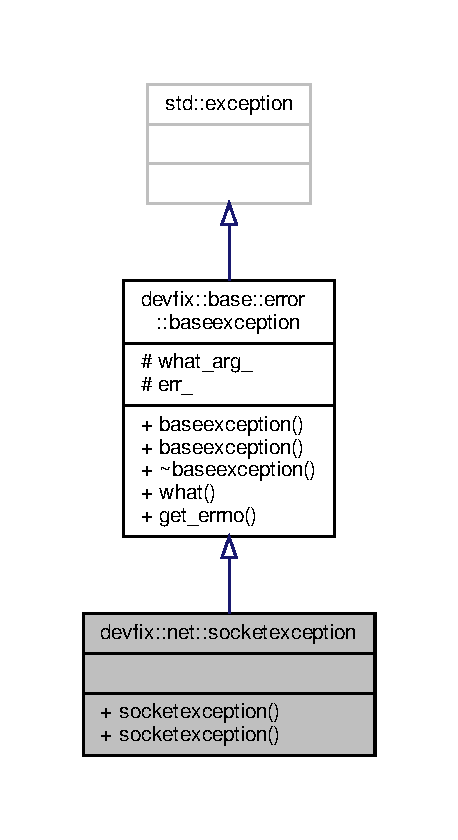
\includegraphics[width=220pt]{structdevfix_1_1net_1_1socketexception__inherit__graph}
\end{center}
\end{figure}
\subsection*{Public Member Functions}
\begin{DoxyCompactItemize}
\item 
\hyperlink{structdevfix_1_1net_1_1socketexception_aeab5d004d494103b37156a5f23a5296a}{socketexception} (const std\+::string \&what\+\_\+arg, int err=-\/1)
\item 
\hyperlink{structdevfix_1_1net_1_1socketexception_a6da69f635eb11f932a0e960545d023bd}{socketexception} (const char $\ast$what\+\_\+arg, int err=-\/1)
\end{DoxyCompactItemize}
\subsection*{Additional Inherited Members}


\subsection{Detailed Description}
Thrown to indicate that there is an error creating or accessing a Socket. 

\subsection{Constructor \& Destructor Documentation}
\mbox{\Hypertarget{structdevfix_1_1net_1_1socketexception_aeab5d004d494103b37156a5f23a5296a}\label{structdevfix_1_1net_1_1socketexception_aeab5d004d494103b37156a5f23a5296a}} 
\index{devfix\+::net\+::socketexception@{devfix\+::net\+::socketexception}!socketexception@{socketexception}}
\index{socketexception@{socketexception}!devfix\+::net\+::socketexception@{devfix\+::net\+::socketexception}}
\subsubsection{\texorpdfstring{socketexception()}{socketexception()}\hspace{0.1cm}{\footnotesize\ttfamily [1/2]}}
{\footnotesize\ttfamily devfix\+::net\+::socketexception\+::socketexception (\begin{DoxyParamCaption}\item[{const std\+::string \&}]{what\+\_\+arg,  }\item[{int}]{err = {\ttfamily -\/1} }\end{DoxyParamCaption})\hspace{0.3cm}{\ttfamily [inline]}, {\ttfamily [explicit]}}

Constructs the error object with what\+\_\+arg as explanatory string that can be accessed through \hyperlink{structdevfix_1_1base_1_1error_1_1baseexception_a16327152a55d65b1e537825231fbd452}{what()}. 
\begin{DoxyParams}{Parameters}
{\em what\+\_\+arg} & explanatory std\+::string \\
\hline
{\em err} & c error code (errno) \\
\hline
\end{DoxyParams}
\mbox{\Hypertarget{structdevfix_1_1net_1_1socketexception_a6da69f635eb11f932a0e960545d023bd}\label{structdevfix_1_1net_1_1socketexception_a6da69f635eb11f932a0e960545d023bd}} 
\index{devfix\+::net\+::socketexception@{devfix\+::net\+::socketexception}!socketexception@{socketexception}}
\index{socketexception@{socketexception}!devfix\+::net\+::socketexception@{devfix\+::net\+::socketexception}}
\subsubsection{\texorpdfstring{socketexception()}{socketexception()}\hspace{0.1cm}{\footnotesize\ttfamily [2/2]}}
{\footnotesize\ttfamily devfix\+::net\+::socketexception\+::socketexception (\begin{DoxyParamCaption}\item[{const char $\ast$}]{what\+\_\+arg,  }\item[{int}]{err = {\ttfamily -\/1} }\end{DoxyParamCaption})\hspace{0.3cm}{\ttfamily [inline]}, {\ttfamily [explicit]}}

Constructs the error object with what\+\_\+arg as explanatory string that can be accessed through \hyperlink{structdevfix_1_1base_1_1error_1_1baseexception_a16327152a55d65b1e537825231fbd452}{what()}. 
\begin{DoxyParams}{Parameters}
{\em what\+\_\+arg} & explanatory c-\/string \\
\hline
{\em err} & c error code (errno) \\
\hline
\end{DoxyParams}


The documentation for this struct was generated from the following file\+:\begin{DoxyCompactItemize}
\item 
devfix/net/\hyperlink{socketexception_8h}{socketexception.\+h}\end{DoxyCompactItemize}

\hypertarget{structdevfix_1_1base_1_1io_1_1source}{}\section{devfix\+:\+:base\+:\+:io\+:\+:source Struct Reference}
\label{structdevfix_1_1base_1_1io_1_1source}\index{devfix\+::base\+::io\+::source@{devfix\+::base\+::io\+::source}}


Inheritance diagram for devfix\+:\+:base\+:\+:io\+:\+:source\+:
% FIG 0


Collaboration diagram for devfix\+:\+:base\+:\+:io\+:\+:source\+:
% FIG 1
\subsection*{Public Member Functions}
\begin{DoxyCompactItemize}
\item 
\mbox{\Hypertarget{structdevfix_1_1base_1_1io_1_1source_af8bef20f5b54153c3fd1fbc7daa263c5}\label{structdevfix_1_1base_1_1io_1_1source_af8bef20f5b54153c3fd1fbc7daa263c5}} 
{\bfseries source} (read\+\_\+t \hyperlink{structdevfix_1_1base_1_1io_1_1source_a9fbd4d20aa150910ced44018e1b3156a}{read}, skip\+\_\+t \hyperlink{structdevfix_1_1base_1_1io_1_1source_a21cb579307589cbc6f9e02d64c66f4b2}{skip}, available\+\_\+t \hyperlink{structdevfix_1_1base_1_1io_1_1source_a911f4ba79499a623de30cf16d3d26d47}{available}, close\+\_\+t \hyperlink{structdevfix_1_1base_1_1io_1_1source_aa00a381c8a166cbbc5dbf6de4b56590e}{close}=D\+E\+F\+A\+U\+L\+T\+\_\+\+C\+L\+O\+SE, is\+\_\+closed\+\_\+t \hyperlink{structdevfix_1_1base_1_1io_1_1source_a406834cf6651d48949b96d0ef49cc6c1}{is\+\_\+closed}=D\+E\+F\+A\+U\+L\+T\+\_\+\+I\+S\+\_\+\+C\+L\+O\+S\+ED)
\item 
void \hyperlink{structdevfix_1_1base_1_1io_1_1source_a9fbd4d20aa150910ced44018e1b3156a}{read} (void $\ast$buf, std\+::size\+\_\+t len) override
\begin{DoxyCompactList}\small\item\em Reads bytes from the input stream and stores them into the buffer. \end{DoxyCompactList}\item 
void \hyperlink{structdevfix_1_1base_1_1io_1_1source_a21cb579307589cbc6f9e02d64c66f4b2}{skip} (std\+::size\+\_\+t n) override
\begin{DoxyCompactList}\small\item\em Skips over and discards n bytes of data from this input stream. \end{DoxyCompactList}\item 
std\+::size\+\_\+t \hyperlink{structdevfix_1_1base_1_1io_1_1source_a911f4ba79499a623de30cf16d3d26d47}{available} () override
\begin{DoxyCompactList}\small\item\em Returns an estimate of the number of bytes that can be read (or skipped over) from this input stream without blocking by the next invocation of a method for this input stream. \end{DoxyCompactList}\item 
void \hyperlink{structdevfix_1_1base_1_1io_1_1source_aa00a381c8a166cbbc5dbf6de4b56590e}{close} () override
\begin{DoxyCompactList}\small\item\em Closes this input stream and releases any system resources associated with the stream. \end{DoxyCompactList}\item 
bool \hyperlink{structdevfix_1_1base_1_1io_1_1source_a406834cf6651d48949b96d0ef49cc6c1}{is\+\_\+closed} () override
\begin{DoxyCompactList}\small\item\em Returns if the {\itshape inputstream} is closed or available for further calls of input operations. \end{DoxyCompactList}\end{DoxyCompactItemize}


\subsection{Member Function Documentation}
\mbox{\Hypertarget{structdevfix_1_1base_1_1io_1_1source_a911f4ba79499a623de30cf16d3d26d47}\label{structdevfix_1_1base_1_1io_1_1source_a911f4ba79499a623de30cf16d3d26d47}} 
\index{devfix\+::base\+::io\+::source@{devfix\+::base\+::io\+::source}!available@{available}}
\index{available@{available}!devfix\+::base\+::io\+::source@{devfix\+::base\+::io\+::source}}
\subsubsection{\texorpdfstring{available()}{available()}}
{\footnotesize\ttfamily std\+::size\+\_\+t devfix\+::base\+::io\+::source\+::available (\begin{DoxyParamCaption}{ }\end{DoxyParamCaption})\hspace{0.3cm}{\ttfamily [override]}, {\ttfamily [virtual]}}



Returns an estimate of the number of bytes that can be read (or skipped over) from this input stream without blocking by the next invocation of a method for this input stream. 

A single read or skip of this many bytes will not block, but may read or skip fewer bytes.

Note that while some implementations of {\itshape inputstream} will return the total number of bytes in the stream, many will not. It is never correct to use the return value of this method to allocate a buffer intended to hold all data in this stream.

A subclass\textquotesingle{} implementation of this method may choose to throw an I\+O\+Exception if this input stream has been closed by invoking the \hyperlink{structdevfix_1_1base_1_1io_1_1source_aa00a381c8a166cbbc5dbf6de4b56590e}{close()} method.

This method should be overridden by subclasses.

\begin{DoxyReturn}{Returns}
an estimate of the number of bytes that can be read (or skipped over) from this input stream without blocking or 0 when it reaches the end of the input stream. 
\end{DoxyReturn}


Implements \hyperlink{structdevfix_1_1base_1_1io_1_1inputstream_ace04813af676b6c81fa452eb4d81a796}{devfix\+::base\+::io\+::inputstream}.

\mbox{\Hypertarget{structdevfix_1_1base_1_1io_1_1source_aa00a381c8a166cbbc5dbf6de4b56590e}\label{structdevfix_1_1base_1_1io_1_1source_aa00a381c8a166cbbc5dbf6de4b56590e}} 
\index{devfix\+::base\+::io\+::source@{devfix\+::base\+::io\+::source}!close@{close}}
\index{close@{close}!devfix\+::base\+::io\+::source@{devfix\+::base\+::io\+::source}}
\subsubsection{\texorpdfstring{close()}{close()}}
{\footnotesize\ttfamily void devfix\+::base\+::io\+::source\+::close (\begin{DoxyParamCaption}{ }\end{DoxyParamCaption})\hspace{0.3cm}{\ttfamily [override]}, {\ttfamily [virtual]}}



Closes this input stream and releases any system resources associated with the stream. 

A closed stream cannot perform input operations and cannot be reopened. 

Implements \hyperlink{structdevfix_1_1base_1_1io_1_1inputstream_a1188eff97757eb9625be91dfeca17af7}{devfix\+::base\+::io\+::inputstream}.

\mbox{\Hypertarget{structdevfix_1_1base_1_1io_1_1source_a406834cf6651d48949b96d0ef49cc6c1}\label{structdevfix_1_1base_1_1io_1_1source_a406834cf6651d48949b96d0ef49cc6c1}} 
\index{devfix\+::base\+::io\+::source@{devfix\+::base\+::io\+::source}!is\+\_\+closed@{is\+\_\+closed}}
\index{is\+\_\+closed@{is\+\_\+closed}!devfix\+::base\+::io\+::source@{devfix\+::base\+::io\+::source}}
\subsubsection{\texorpdfstring{is\+\_\+closed()}{is\_closed()}}
{\footnotesize\ttfamily bool devfix\+::base\+::io\+::source\+::is\+\_\+closed (\begin{DoxyParamCaption}{ }\end{DoxyParamCaption})\hspace{0.3cm}{\ttfamily [override]}, {\ttfamily [virtual]}}



Returns if the {\itshape inputstream} is closed or available for further calls of input operations. 

\begin{DoxyReturn}{Returns}
true if the {\itshape inputstream} got previously closed. 
\end{DoxyReturn}


Implements \hyperlink{structdevfix_1_1base_1_1io_1_1inputstream_a9da6b400424ff476ed0479193c219fa9}{devfix\+::base\+::io\+::inputstream}.

\mbox{\Hypertarget{structdevfix_1_1base_1_1io_1_1source_a9fbd4d20aa150910ced44018e1b3156a}\label{structdevfix_1_1base_1_1io_1_1source_a9fbd4d20aa150910ced44018e1b3156a}} 
\index{devfix\+::base\+::io\+::source@{devfix\+::base\+::io\+::source}!read@{read}}
\index{read@{read}!devfix\+::base\+::io\+::source@{devfix\+::base\+::io\+::source}}
\subsubsection{\texorpdfstring{read()}{read()}}
{\footnotesize\ttfamily void devfix\+::base\+::io\+::source\+::read (\begin{DoxyParamCaption}\item[{void $\ast$}]{buf,  }\item[{std\+::size\+\_\+t}]{len }\end{DoxyParamCaption})\hspace{0.3cm}{\ttfamily [override]}, {\ttfamily [virtual]}}



Reads bytes from the input stream and stores them into the buffer. 

This method blocks until input data is available, end of file is detected, or another exception is thrown.

If len is zero, then no bytes are read. If no byte is available because the stream is at end of file, an exception is thrown.

The first byte read is stored into element b\mbox{[}0\mbox{]}, the next one into b\mbox{[}1\mbox{]}, and so on. If no exception was thrown, the number of bytes read is always equal to len.

Subclasses are encouraged to provide a more efficient implementation of this method.


\begin{DoxyParams}{Parameters}
{\em buf} & the buffer into which the data is read. \\
\hline
{\em len} & the maximum number of bytes to read. \\
\hline
\end{DoxyParams}


Implements \hyperlink{structdevfix_1_1base_1_1io_1_1inputstream_a17e1a21881ae263650ebdaafaee2e71a}{devfix\+::base\+::io\+::inputstream}.

\mbox{\Hypertarget{structdevfix_1_1base_1_1io_1_1source_a21cb579307589cbc6f9e02d64c66f4b2}\label{structdevfix_1_1base_1_1io_1_1source_a21cb579307589cbc6f9e02d64c66f4b2}} 
\index{devfix\+::base\+::io\+::source@{devfix\+::base\+::io\+::source}!skip@{skip}}
\index{skip@{skip}!devfix\+::base\+::io\+::source@{devfix\+::base\+::io\+::source}}
\subsubsection{\texorpdfstring{skip()}{skip()}}
{\footnotesize\ttfamily void devfix\+::base\+::io\+::source\+::skip (\begin{DoxyParamCaption}\item[{std\+::size\+\_\+t}]{n }\end{DoxyParamCaption})\hspace{0.3cm}{\ttfamily [override]}, {\ttfamily [virtual]}}



Skips over and discards n bytes of data from this input stream. 

The skip method may, for a variety of reasons, end up skipping over some smaller number of bytes, possibly 0. This may result from any of a number of conditions; reaching end of file before n bytes have been skipped is only one possibility.


\begin{DoxyParams}{Parameters}
{\em n} & the number of bytes to be skipped. \\
\hline
\end{DoxyParams}


Implements \hyperlink{structdevfix_1_1base_1_1io_1_1inputstream_a1868a733fd646b29daae6874e07e4e03}{devfix\+::base\+::io\+::inputstream}.



The documentation for this struct was generated from the following files\+:\begin{DoxyCompactItemize}
\item 
devfix/base/io/source.\+h\item 
devfix/base/io/source.\+cpp\end{DoxyCompactItemize}

\hypertarget{structdevfix_1_1dsp_1_1spectrogram}{}\section{devfix\+:\+:dsp\+:\+:spectrogram$<$ FloatT, N, win\+\_\+fun $>$ Struct Template Reference}
\label{structdevfix_1_1dsp_1_1spectrogram}\index{devfix\+::dsp\+::spectrogram$<$ Float\+T, N, win\+\_\+fun $>$@{devfix\+::dsp\+::spectrogram$<$ Float\+T, N, win\+\_\+fun $>$}}


{\ttfamily \#include $<$spectrogram.\+h$>$}

\subsection*{Public Types}
\begin{DoxyCompactItemize}
\item 
using \hyperlink{structdevfix_1_1dsp_1_1spectrogram_a920fdda446509cfe81fa287773c709cb}{complex\+\_\+t} = std\+::complex$<$ FloatT $>$
\end{DoxyCompactItemize}
\subsection*{Public Member Functions}
\begin{DoxyCompactItemize}
\item 
\hyperlink{structdevfix_1_1dsp_1_1spectrogram_ad1d11586447533319ec37e5e9de6e6e9}{spectrogram} (std\+::size\+\_\+t window\+\_\+distance)
\item 
void \hyperlink{structdevfix_1_1dsp_1_1spectrogram_a9204dfb17067382f9e01295bc349d4f1}{add} (const \hyperlink{structdevfix_1_1dsp_1_1spectrogram_a920fdda446509cfe81fa287773c709cb}{complex\+\_\+t} $\ast$data, std\+::size\+\_\+t len)
\item 
void \hyperlink{structdevfix_1_1dsp_1_1spectrogram_abf5e5730f6248014f7ee5a22a0e96662}{add} (const std\+::vector$<$ \hyperlink{structdevfix_1_1dsp_1_1spectrogram_a920fdda446509cfe81fa287773c709cb}{complex\+\_\+t} $>$ \&vec)
\item 
{\footnotesize template$<$std\+::size\+\_\+t N\+\_\+elems$>$ }\\void \hyperlink{structdevfix_1_1dsp_1_1spectrogram_a030123c941c6acc6ea535514c2d138da}{add} (const std\+::array$<$ \hyperlink{structdevfix_1_1dsp_1_1spectrogram_a920fdda446509cfe81fa287773c709cb}{complex\+\_\+t}, N\+\_\+elems $>$ \&arr)
\item 
std\+::array$<$ \hyperlink{structdevfix_1_1dsp_1_1spectrogram_a920fdda446509cfe81fa287773c709cb}{complex\+\_\+t}, N $>$ \hyperlink{structdevfix_1_1dsp_1_1spectrogram_acdc5a2253a62ae50ae24607cd4f3b555}{pop} ()
\item 
std\+::size\+\_\+t \hyperlink{structdevfix_1_1dsp_1_1spectrogram_a6dc48452751bc4b4f4e14088998ddbb7}{size} () const
\end{DoxyCompactItemize}


\subsection{Member Typedef Documentation}
\mbox{\Hypertarget{structdevfix_1_1dsp_1_1spectrogram_a920fdda446509cfe81fa287773c709cb}\label{structdevfix_1_1dsp_1_1spectrogram_a920fdda446509cfe81fa287773c709cb}} 
\index{devfix\+::dsp\+::spectrogram@{devfix\+::dsp\+::spectrogram}!complex\+\_\+t@{complex\+\_\+t}}
\index{complex\+\_\+t@{complex\+\_\+t}!devfix\+::dsp\+::spectrogram@{devfix\+::dsp\+::spectrogram}}
\subsubsection{\texorpdfstring{complex\+\_\+t}{complex\_t}}
{\footnotesize\ttfamily template$<$typename FloatT, std\+::size\+\_\+t N, Float\+T($\ast$)(std\+::size\+\_\+t, std\+::size\+\_\+t) win\+\_\+fun$>$ \\
using \hyperlink{structdevfix_1_1dsp_1_1spectrogram}{devfix\+::dsp\+::spectrogram}$<$ FloatT, N, win\+\_\+fun $>$\+::\hyperlink{structdevfix_1_1dsp_1_1spectrogram_a920fdda446509cfe81fa287773c709cb}{complex\+\_\+t} =  std\+::complex$<$FloatT$>$}



\subsection{Constructor \& Destructor Documentation}
\mbox{\Hypertarget{structdevfix_1_1dsp_1_1spectrogram_ad1d11586447533319ec37e5e9de6e6e9}\label{structdevfix_1_1dsp_1_1spectrogram_ad1d11586447533319ec37e5e9de6e6e9}} 
\index{devfix\+::dsp\+::spectrogram@{devfix\+::dsp\+::spectrogram}!spectrogram@{spectrogram}}
\index{spectrogram@{spectrogram}!devfix\+::dsp\+::spectrogram@{devfix\+::dsp\+::spectrogram}}
\subsubsection{\texorpdfstring{spectrogram()}{spectrogram()}}
{\footnotesize\ttfamily template$<$typename FloatT, std\+::size\+\_\+t N, Float\+T($\ast$)(std\+::size\+\_\+t, std\+::size\+\_\+t) win\+\_\+fun$>$ \\
\hyperlink{structdevfix_1_1dsp_1_1spectrogram}{devfix\+::dsp\+::spectrogram}$<$ FloatT, N, win\+\_\+fun $>$\+::\hyperlink{structdevfix_1_1dsp_1_1spectrogram}{spectrogram} (\begin{DoxyParamCaption}\item[{std\+::size\+\_\+t}]{window\+\_\+distance }\end{DoxyParamCaption})\hspace{0.3cm}{\ttfamily [inline]}, {\ttfamily [explicit]}}



\subsection{Member Function Documentation}
\mbox{\Hypertarget{structdevfix_1_1dsp_1_1spectrogram_a9204dfb17067382f9e01295bc349d4f1}\label{structdevfix_1_1dsp_1_1spectrogram_a9204dfb17067382f9e01295bc349d4f1}} 
\index{devfix\+::dsp\+::spectrogram@{devfix\+::dsp\+::spectrogram}!add@{add}}
\index{add@{add}!devfix\+::dsp\+::spectrogram@{devfix\+::dsp\+::spectrogram}}
\subsubsection{\texorpdfstring{add()}{add()}\hspace{0.1cm}{\footnotesize\ttfamily [1/3]}}
{\footnotesize\ttfamily template$<$typename FloatT, std\+::size\+\_\+t N, Float\+T($\ast$)(std\+::size\+\_\+t, std\+::size\+\_\+t) win\+\_\+fun$>$ \\
void \hyperlink{structdevfix_1_1dsp_1_1spectrogram}{devfix\+::dsp\+::spectrogram}$<$ FloatT, N, win\+\_\+fun $>$\+::add (\begin{DoxyParamCaption}\item[{const \hyperlink{structdevfix_1_1dsp_1_1spectrogram_a920fdda446509cfe81fa287773c709cb}{complex\+\_\+t} $\ast$}]{data,  }\item[{std\+::size\+\_\+t}]{len }\end{DoxyParamCaption})\hspace{0.3cm}{\ttfamily [inline]}}

Here is the caller graph for this function\+:\nopagebreak
\begin{figure}[H]
\begin{center}
\leavevmode
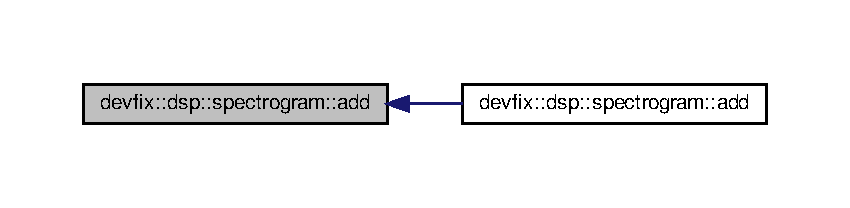
\includegraphics[width=350pt]{structdevfix_1_1dsp_1_1spectrogram_a9204dfb17067382f9e01295bc349d4f1_icgraph}
\end{center}
\end{figure}
\mbox{\Hypertarget{structdevfix_1_1dsp_1_1spectrogram_abf5e5730f6248014f7ee5a22a0e96662}\label{structdevfix_1_1dsp_1_1spectrogram_abf5e5730f6248014f7ee5a22a0e96662}} 
\index{devfix\+::dsp\+::spectrogram@{devfix\+::dsp\+::spectrogram}!add@{add}}
\index{add@{add}!devfix\+::dsp\+::spectrogram@{devfix\+::dsp\+::spectrogram}}
\subsubsection{\texorpdfstring{add()}{add()}\hspace{0.1cm}{\footnotesize\ttfamily [2/3]}}
{\footnotesize\ttfamily template$<$typename FloatT, std\+::size\+\_\+t N, Float\+T($\ast$)(std\+::size\+\_\+t, std\+::size\+\_\+t) win\+\_\+fun$>$ \\
void \hyperlink{structdevfix_1_1dsp_1_1spectrogram}{devfix\+::dsp\+::spectrogram}$<$ FloatT, N, win\+\_\+fun $>$\+::add (\begin{DoxyParamCaption}\item[{const std\+::vector$<$ \hyperlink{structdevfix_1_1dsp_1_1spectrogram_a920fdda446509cfe81fa287773c709cb}{complex\+\_\+t} $>$ \&}]{vec }\end{DoxyParamCaption})\hspace{0.3cm}{\ttfamily [inline]}}

\mbox{\Hypertarget{structdevfix_1_1dsp_1_1spectrogram_a030123c941c6acc6ea535514c2d138da}\label{structdevfix_1_1dsp_1_1spectrogram_a030123c941c6acc6ea535514c2d138da}} 
\index{devfix\+::dsp\+::spectrogram@{devfix\+::dsp\+::spectrogram}!add@{add}}
\index{add@{add}!devfix\+::dsp\+::spectrogram@{devfix\+::dsp\+::spectrogram}}
\subsubsection{\texorpdfstring{add()}{add()}\hspace{0.1cm}{\footnotesize\ttfamily [3/3]}}
{\footnotesize\ttfamily template$<$typename FloatT, std\+::size\+\_\+t N, Float\+T($\ast$)(std\+::size\+\_\+t, std\+::size\+\_\+t) win\+\_\+fun$>$ \\
template$<$std\+::size\+\_\+t N\+\_\+elems$>$ \\
void \hyperlink{structdevfix_1_1dsp_1_1spectrogram}{devfix\+::dsp\+::spectrogram}$<$ FloatT, N, win\+\_\+fun $>$\+::add (\begin{DoxyParamCaption}\item[{const std\+::array$<$ \hyperlink{structdevfix_1_1dsp_1_1spectrogram_a920fdda446509cfe81fa287773c709cb}{complex\+\_\+t}, N\+\_\+elems $>$ \&}]{arr }\end{DoxyParamCaption})\hspace{0.3cm}{\ttfamily [inline]}}

\mbox{\Hypertarget{structdevfix_1_1dsp_1_1spectrogram_acdc5a2253a62ae50ae24607cd4f3b555}\label{structdevfix_1_1dsp_1_1spectrogram_acdc5a2253a62ae50ae24607cd4f3b555}} 
\index{devfix\+::dsp\+::spectrogram@{devfix\+::dsp\+::spectrogram}!pop@{pop}}
\index{pop@{pop}!devfix\+::dsp\+::spectrogram@{devfix\+::dsp\+::spectrogram}}
\subsubsection{\texorpdfstring{pop()}{pop()}}
{\footnotesize\ttfamily template$<$typename FloatT, std\+::size\+\_\+t N, Float\+T($\ast$)(std\+::size\+\_\+t, std\+::size\+\_\+t) win\+\_\+fun$>$ \\
std\+::array$<$\hyperlink{structdevfix_1_1dsp_1_1spectrogram_a920fdda446509cfe81fa287773c709cb}{complex\+\_\+t}, N$>$ \hyperlink{structdevfix_1_1dsp_1_1spectrogram}{devfix\+::dsp\+::spectrogram}$<$ FloatT, N, win\+\_\+fun $>$\+::pop (\begin{DoxyParamCaption}{ }\end{DoxyParamCaption})\hspace{0.3cm}{\ttfamily [inline]}}

\mbox{\Hypertarget{structdevfix_1_1dsp_1_1spectrogram_a6dc48452751bc4b4f4e14088998ddbb7}\label{structdevfix_1_1dsp_1_1spectrogram_a6dc48452751bc4b4f4e14088998ddbb7}} 
\index{devfix\+::dsp\+::spectrogram@{devfix\+::dsp\+::spectrogram}!size@{size}}
\index{size@{size}!devfix\+::dsp\+::spectrogram@{devfix\+::dsp\+::spectrogram}}
\subsubsection{\texorpdfstring{size()}{size()}}
{\footnotesize\ttfamily template$<$typename FloatT, std\+::size\+\_\+t N, Float\+T($\ast$)(std\+::size\+\_\+t, std\+::size\+\_\+t) win\+\_\+fun$>$ \\
std\+::size\+\_\+t \hyperlink{structdevfix_1_1dsp_1_1spectrogram}{devfix\+::dsp\+::spectrogram}$<$ FloatT, N, win\+\_\+fun $>$\+::size (\begin{DoxyParamCaption}{ }\end{DoxyParamCaption}) const\hspace{0.3cm}{\ttfamily [inline]}}



The documentation for this struct was generated from the following file\+:\begin{DoxyCompactItemize}
\item 
devfix/dsp/\hyperlink{spectrogram_8h}{spectrogram.\+h}\end{DoxyCompactItemize}

\hypertarget{structdevfix_1_1base_1_1strout}{}\section{devfix\+:\+:base\+:\+:strout$<$ CharT, Traits, Allocator $>$ Struct Template Reference}
\label{structdevfix_1_1base_1_1strout}\index{devfix\+::base\+::strout$<$ Char\+T, Traits, Allocator $>$@{devfix\+::base\+::strout$<$ Char\+T, Traits, Allocator $>$}}


{\ttfamily \#include $<$strout.\+h$>$}



Inheritance diagram for devfix\+:\+:base\+:\+:strout$<$ CharT, Traits, Allocator $>$\+:\nopagebreak
\begin{figure}[H]
\begin{center}
\leavevmode
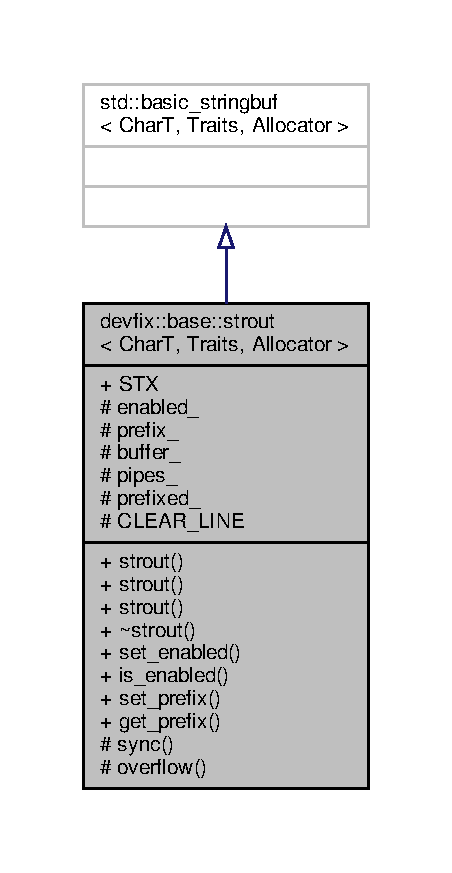
\includegraphics[width=217pt]{structdevfix_1_1base_1_1strout__inherit__graph}
\end{center}
\end{figure}
\subsection*{Public Types}
\begin{DoxyCompactItemize}
\item 
using \hyperlink{structdevfix_1_1base_1_1strout_a89bb8340fe2e43bb14c829a1d427d9c0}{pipe\+\_\+fun\+\_\+t} = std\+::function$<$ void(const std\+::basic\+\_\+string$<$ CharT $>$ \&)$>$
\item 
using \hyperlink{structdevfix_1_1base_1_1strout_ad6cf2897069f246b884fa8d526f8bab1}{flush\+\_\+fun\+\_\+t} = std\+::function$<$ void()$>$
\item 
using \hyperlink{structdevfix_1_1base_1_1strout_a2212cb8a99abec10490e891cc67820bb}{pair\+\_\+t} = std\+::pair$<$ \hyperlink{structdevfix_1_1base_1_1strout_a89bb8340fe2e43bb14c829a1d427d9c0}{pipe\+\_\+fun\+\_\+t}, \hyperlink{structdevfix_1_1base_1_1strout_ad6cf2897069f246b884fa8d526f8bab1}{flush\+\_\+fun\+\_\+t} $>$
\item 
using \hyperlink{structdevfix_1_1base_1_1strout_a158aadfad348eeac7c56a8b43699a4d3}{stream\+\_\+t} = std\+::basic\+\_\+ostream$<$ CharT $>$
\item 
using \hyperlink{structdevfix_1_1base_1_1strout_acf852ff3e37e6d10e2cf0332df2b8e2d}{pipes\+\_\+t} = std\+::vector$<$ std\+::variant$<$ \hyperlink{structdevfix_1_1base_1_1strout_a158aadfad348eeac7c56a8b43699a4d3}{stream\+\_\+t} $\ast$, \hyperlink{structdevfix_1_1base_1_1strout_a2212cb8a99abec10490e891cc67820bb}{pair\+\_\+t} $>$ $>$
\end{DoxyCompactItemize}
\subsection*{Public Member Functions}
\begin{DoxyCompactItemize}
\item 
\hyperlink{structdevfix_1_1base_1_1strout_a7711671b7f3457ed5cc509f7d7c7239f}{strout} (\hyperlink{structdevfix_1_1base_1_1strout_acf852ff3e37e6d10e2cf0332df2b8e2d}{pipes\+\_\+t} pipes)
\item 
\hyperlink{structdevfix_1_1base_1_1strout_a87b4c01cbcd87414d2c3a639713fcd08}{strout} (\hyperlink{structdevfix_1_1base_1_1strout_a158aadfad348eeac7c56a8b43699a4d3}{stream\+\_\+t} $\ast$stream)
\item 
\hyperlink{structdevfix_1_1base_1_1strout_a83d80540c9614d8d825a45acede871c5}{strout} (\hyperlink{structdevfix_1_1base_1_1strout_a2212cb8a99abec10490e891cc67820bb}{pair\+\_\+t} pair)
\item 
\hyperlink{structdevfix_1_1base_1_1strout_aeffa562814f23e6e74f5d8404d673ea7}{$\sim$strout} ()
\item 
void \hyperlink{structdevfix_1_1base_1_1strout_a49000248c873a593348082f151ccab9b}{set\+\_\+enabled} (bool enabled)
\item 
bool \hyperlink{structdevfix_1_1base_1_1strout_a62b7808c3d8b54dd926bdecabea7cbd2}{is\+\_\+enabled} () const
\item 
void \hyperlink{structdevfix_1_1base_1_1strout_ab32a1f2eb733dcba516e439f651f5910}{set\+\_\+prefix} (const std\+::basic\+\_\+string$<$ CharT $>$ \&prefix)
\item 
const std\+::basic\+\_\+string$<$ CharT $>$ \& \hyperlink{structdevfix_1_1base_1_1strout_afb40810ea1e7384f08e1f837e34ff1c2}{get\+\_\+prefix} () const
\end{DoxyCompactItemize}
\subsection*{Static Public Attributes}
\begin{DoxyCompactItemize}
\item 
static constexpr CharT \hyperlink{structdevfix_1_1base_1_1strout_a76183010a1d8e9360e34b9cd9ab33f7d}{S\+TX} = static\+\_\+cast$<$CharT$>$(\textquotesingle{}\textbackslash{}x02\textquotesingle{})
\begin{DoxyCompactList}\small\item\em Start of Text, clear whole line before new text gets displayed. \end{DoxyCompactList}\end{DoxyCompactItemize}
\subsection*{Protected Types}
\begin{DoxyCompactItemize}
\item 
using \hyperlink{structdevfix_1_1base_1_1strout_ac08d70e3105ac2175c26e34818624826}{int\+\_\+type} = typename std\+::basic\+\_\+stringbuf$<$ CharT, Traits, Allocator $>$\+::\hyperlink{structdevfix_1_1base_1_1strout_ac08d70e3105ac2175c26e34818624826}{int\+\_\+type}
\end{DoxyCompactItemize}
\subsection*{Protected Member Functions}
\begin{DoxyCompactItemize}
\item 
int \hyperlink{structdevfix_1_1base_1_1strout_a50b305dcf9905bfe75fa1bba42718169}{sync} () override
\item 
\hyperlink{structdevfix_1_1base_1_1strout_ac08d70e3105ac2175c26e34818624826}{int\+\_\+type} \hyperlink{structdevfix_1_1base_1_1strout_a1d8ba6e5c7c0c2d5558095d957cc4273}{overflow} (\hyperlink{structdevfix_1_1base_1_1strout_ac08d70e3105ac2175c26e34818624826}{int\+\_\+type} c) override
\end{DoxyCompactItemize}
\subsection*{Protected Attributes}
\begin{DoxyCompactItemize}
\item 
bool \hyperlink{structdevfix_1_1base_1_1strout_a813fc6630d6565cf5a00e620b536671c}{enabled\+\_\+} = true
\item 
std\+::basic\+\_\+string$<$ CharT $>$ \hyperlink{structdevfix_1_1base_1_1strout_a664c76563ab0f7f0625779aaf0c56395}{prefix\+\_\+}
\item 
std\+::basic\+\_\+stringstream$<$ CharT $>$ \hyperlink{structdevfix_1_1base_1_1strout_a0625f5cbd10441a4613bf3aae5ab15a1}{buffer\+\_\+}
\item 
std\+::vector$<$ std\+::variant$<$ \hyperlink{structdevfix_1_1base_1_1strout_a158aadfad348eeac7c56a8b43699a4d3}{stream\+\_\+t} $\ast$, \hyperlink{structdevfix_1_1base_1_1strout_a2212cb8a99abec10490e891cc67820bb}{pair\+\_\+t} $>$ $>$ \hyperlink{structdevfix_1_1base_1_1strout_aa92f98e253e448a0ea897760764486e7}{pipes\+\_\+}
\item 
bool \hyperlink{structdevfix_1_1base_1_1strout_a1e56005b02772de34fddd5e4f44741c3}{prefixed\+\_\+} = true
\end{DoxyCompactItemize}
\subsection*{Static Protected Attributes}
\begin{DoxyCompactItemize}
\item 
static constexpr std\+::basic\+\_\+string\+\_\+view$<$ CharT $>$ \hyperlink{structdevfix_1_1base_1_1strout_afe9d2f4264b508fd02be4af24dba6bb1}{C\+L\+E\+A\+R\+\_\+\+L\+I\+NE} = \hyperlink{strutil_8h_a72f64e8a28f366adf3cad6c109082271}{M\+U\+L\+T\+I\+S\+T\+R\+I\+NG}(CharT, \char`\"{}\textbackslash{}033\mbox{[}2\+K\textbackslash{}r\char`\"{})
\end{DoxyCompactItemize}


\subsection{Member Typedef Documentation}
\mbox{\Hypertarget{structdevfix_1_1base_1_1strout_ad6cf2897069f246b884fa8d526f8bab1}\label{structdevfix_1_1base_1_1strout_ad6cf2897069f246b884fa8d526f8bab1}} 
\index{devfix\+::base\+::strout@{devfix\+::base\+::strout}!flush\+\_\+fun\+\_\+t@{flush\+\_\+fun\+\_\+t}}
\index{flush\+\_\+fun\+\_\+t@{flush\+\_\+fun\+\_\+t}!devfix\+::base\+::strout@{devfix\+::base\+::strout}}
\subsubsection{\texorpdfstring{flush\+\_\+fun\+\_\+t}{flush\_fun\_t}}
{\footnotesize\ttfamily template$<$class CharT, class Traits = std\+::char\+\_\+traits$<$\+Char\+T$>$, class Allocator = std\+::allocator$<$\+Char\+T$>$$>$ \\
using \hyperlink{structdevfix_1_1base_1_1strout}{devfix\+::base\+::strout}$<$ CharT, Traits, Allocator $>$\+::\hyperlink{structdevfix_1_1base_1_1strout_ad6cf2897069f246b884fa8d526f8bab1}{flush\+\_\+fun\+\_\+t} =  std\+::function$<$void()$>$}

\mbox{\Hypertarget{structdevfix_1_1base_1_1strout_ac08d70e3105ac2175c26e34818624826}\label{structdevfix_1_1base_1_1strout_ac08d70e3105ac2175c26e34818624826}} 
\index{devfix\+::base\+::strout@{devfix\+::base\+::strout}!int\+\_\+type@{int\+\_\+type}}
\index{int\+\_\+type@{int\+\_\+type}!devfix\+::base\+::strout@{devfix\+::base\+::strout}}
\subsubsection{\texorpdfstring{int\+\_\+type}{int\_type}}
{\footnotesize\ttfamily template$<$class CharT, class Traits = std\+::char\+\_\+traits$<$\+Char\+T$>$, class Allocator = std\+::allocator$<$\+Char\+T$>$$>$ \\
using \hyperlink{structdevfix_1_1base_1_1strout}{devfix\+::base\+::strout}$<$ CharT, Traits, Allocator $>$\+::\hyperlink{structdevfix_1_1base_1_1strout_ac08d70e3105ac2175c26e34818624826}{int\+\_\+type} =  typename std\+::basic\+\_\+stringbuf$<$CharT, Traits, Allocator$>$\+::\hyperlink{structdevfix_1_1base_1_1strout_ac08d70e3105ac2175c26e34818624826}{int\+\_\+type}\hspace{0.3cm}{\ttfamily [protected]}}

\mbox{\Hypertarget{structdevfix_1_1base_1_1strout_a2212cb8a99abec10490e891cc67820bb}\label{structdevfix_1_1base_1_1strout_a2212cb8a99abec10490e891cc67820bb}} 
\index{devfix\+::base\+::strout@{devfix\+::base\+::strout}!pair\+\_\+t@{pair\+\_\+t}}
\index{pair\+\_\+t@{pair\+\_\+t}!devfix\+::base\+::strout@{devfix\+::base\+::strout}}
\subsubsection{\texorpdfstring{pair\+\_\+t}{pair\_t}}
{\footnotesize\ttfamily template$<$class CharT, class Traits = std\+::char\+\_\+traits$<$\+Char\+T$>$, class Allocator = std\+::allocator$<$\+Char\+T$>$$>$ \\
using \hyperlink{structdevfix_1_1base_1_1strout}{devfix\+::base\+::strout}$<$ CharT, Traits, Allocator $>$\+::\hyperlink{structdevfix_1_1base_1_1strout_a2212cb8a99abec10490e891cc67820bb}{pair\+\_\+t} =  std\+::pair$<$\hyperlink{structdevfix_1_1base_1_1strout_a89bb8340fe2e43bb14c829a1d427d9c0}{pipe\+\_\+fun\+\_\+t}, \hyperlink{structdevfix_1_1base_1_1strout_ad6cf2897069f246b884fa8d526f8bab1}{flush\+\_\+fun\+\_\+t}$>$}

\mbox{\Hypertarget{structdevfix_1_1base_1_1strout_a89bb8340fe2e43bb14c829a1d427d9c0}\label{structdevfix_1_1base_1_1strout_a89bb8340fe2e43bb14c829a1d427d9c0}} 
\index{devfix\+::base\+::strout@{devfix\+::base\+::strout}!pipe\+\_\+fun\+\_\+t@{pipe\+\_\+fun\+\_\+t}}
\index{pipe\+\_\+fun\+\_\+t@{pipe\+\_\+fun\+\_\+t}!devfix\+::base\+::strout@{devfix\+::base\+::strout}}
\subsubsection{\texorpdfstring{pipe\+\_\+fun\+\_\+t}{pipe\_fun\_t}}
{\footnotesize\ttfamily template$<$class CharT, class Traits = std\+::char\+\_\+traits$<$\+Char\+T$>$, class Allocator = std\+::allocator$<$\+Char\+T$>$$>$ \\
using \hyperlink{structdevfix_1_1base_1_1strout}{devfix\+::base\+::strout}$<$ CharT, Traits, Allocator $>$\+::\hyperlink{structdevfix_1_1base_1_1strout_a89bb8340fe2e43bb14c829a1d427d9c0}{pipe\+\_\+fun\+\_\+t} =  std\+::function$<$void(const std\+::basic\+\_\+string$<$CharT$>$\&)$>$}

\mbox{\Hypertarget{structdevfix_1_1base_1_1strout_acf852ff3e37e6d10e2cf0332df2b8e2d}\label{structdevfix_1_1base_1_1strout_acf852ff3e37e6d10e2cf0332df2b8e2d}} 
\index{devfix\+::base\+::strout@{devfix\+::base\+::strout}!pipes\+\_\+t@{pipes\+\_\+t}}
\index{pipes\+\_\+t@{pipes\+\_\+t}!devfix\+::base\+::strout@{devfix\+::base\+::strout}}
\subsubsection{\texorpdfstring{pipes\+\_\+t}{pipes\_t}}
{\footnotesize\ttfamily template$<$class CharT, class Traits = std\+::char\+\_\+traits$<$\+Char\+T$>$, class Allocator = std\+::allocator$<$\+Char\+T$>$$>$ \\
using \hyperlink{structdevfix_1_1base_1_1strout}{devfix\+::base\+::strout}$<$ CharT, Traits, Allocator $>$\+::\hyperlink{structdevfix_1_1base_1_1strout_acf852ff3e37e6d10e2cf0332df2b8e2d}{pipes\+\_\+t} =  std\+::vector$<$std\+::variant$<$\hyperlink{structdevfix_1_1base_1_1strout_a158aadfad348eeac7c56a8b43699a4d3}{stream\+\_\+t}$\ast$, \hyperlink{structdevfix_1_1base_1_1strout_a2212cb8a99abec10490e891cc67820bb}{pair\+\_\+t}$>$ $>$}

\mbox{\Hypertarget{structdevfix_1_1base_1_1strout_a158aadfad348eeac7c56a8b43699a4d3}\label{structdevfix_1_1base_1_1strout_a158aadfad348eeac7c56a8b43699a4d3}} 
\index{devfix\+::base\+::strout@{devfix\+::base\+::strout}!stream\+\_\+t@{stream\+\_\+t}}
\index{stream\+\_\+t@{stream\+\_\+t}!devfix\+::base\+::strout@{devfix\+::base\+::strout}}
\subsubsection{\texorpdfstring{stream\+\_\+t}{stream\_t}}
{\footnotesize\ttfamily template$<$class CharT, class Traits = std\+::char\+\_\+traits$<$\+Char\+T$>$, class Allocator = std\+::allocator$<$\+Char\+T$>$$>$ \\
using \hyperlink{structdevfix_1_1base_1_1strout}{devfix\+::base\+::strout}$<$ CharT, Traits, Allocator $>$\+::\hyperlink{structdevfix_1_1base_1_1strout_a158aadfad348eeac7c56a8b43699a4d3}{stream\+\_\+t} =  std\+::basic\+\_\+ostream$<$CharT$>$}



\subsection{Constructor \& Destructor Documentation}
\mbox{\Hypertarget{structdevfix_1_1base_1_1strout_a7711671b7f3457ed5cc509f7d7c7239f}\label{structdevfix_1_1base_1_1strout_a7711671b7f3457ed5cc509f7d7c7239f}} 
\index{devfix\+::base\+::strout@{devfix\+::base\+::strout}!strout@{strout}}
\index{strout@{strout}!devfix\+::base\+::strout@{devfix\+::base\+::strout}}
\subsubsection{\texorpdfstring{strout()}{strout()}\hspace{0.1cm}{\footnotesize\ttfamily [1/3]}}
{\footnotesize\ttfamily template$<$class CharT, class Traits = std\+::char\+\_\+traits$<$\+Char\+T$>$, class Allocator = std\+::allocator$<$\+Char\+T$>$$>$ \\
\hyperlink{structdevfix_1_1base_1_1strout}{devfix\+::base\+::strout}$<$ CharT, Traits, Allocator $>$\+::\hyperlink{structdevfix_1_1base_1_1strout}{strout} (\begin{DoxyParamCaption}\item[{\hyperlink{structdevfix_1_1base_1_1strout_acf852ff3e37e6d10e2cf0332df2b8e2d}{pipes\+\_\+t}}]{pipes }\end{DoxyParamCaption})\hspace{0.3cm}{\ttfamily [inline]}, {\ttfamily [explicit]}}

\mbox{\Hypertarget{structdevfix_1_1base_1_1strout_a87b4c01cbcd87414d2c3a639713fcd08}\label{structdevfix_1_1base_1_1strout_a87b4c01cbcd87414d2c3a639713fcd08}} 
\index{devfix\+::base\+::strout@{devfix\+::base\+::strout}!strout@{strout}}
\index{strout@{strout}!devfix\+::base\+::strout@{devfix\+::base\+::strout}}
\subsubsection{\texorpdfstring{strout()}{strout()}\hspace{0.1cm}{\footnotesize\ttfamily [2/3]}}
{\footnotesize\ttfamily template$<$class CharT, class Traits = std\+::char\+\_\+traits$<$\+Char\+T$>$, class Allocator = std\+::allocator$<$\+Char\+T$>$$>$ \\
\hyperlink{structdevfix_1_1base_1_1strout}{devfix\+::base\+::strout}$<$ CharT, Traits, Allocator $>$\+::\hyperlink{structdevfix_1_1base_1_1strout}{strout} (\begin{DoxyParamCaption}\item[{\hyperlink{structdevfix_1_1base_1_1strout_a158aadfad348eeac7c56a8b43699a4d3}{stream\+\_\+t} $\ast$}]{stream }\end{DoxyParamCaption})\hspace{0.3cm}{\ttfamily [inline]}, {\ttfamily [explicit]}}

\mbox{\Hypertarget{structdevfix_1_1base_1_1strout_a83d80540c9614d8d825a45acede871c5}\label{structdevfix_1_1base_1_1strout_a83d80540c9614d8d825a45acede871c5}} 
\index{devfix\+::base\+::strout@{devfix\+::base\+::strout}!strout@{strout}}
\index{strout@{strout}!devfix\+::base\+::strout@{devfix\+::base\+::strout}}
\subsubsection{\texorpdfstring{strout()}{strout()}\hspace{0.1cm}{\footnotesize\ttfamily [3/3]}}
{\footnotesize\ttfamily template$<$class CharT, class Traits = std\+::char\+\_\+traits$<$\+Char\+T$>$, class Allocator = std\+::allocator$<$\+Char\+T$>$$>$ \\
\hyperlink{structdevfix_1_1base_1_1strout}{devfix\+::base\+::strout}$<$ CharT, Traits, Allocator $>$\+::\hyperlink{structdevfix_1_1base_1_1strout}{strout} (\begin{DoxyParamCaption}\item[{\hyperlink{structdevfix_1_1base_1_1strout_a2212cb8a99abec10490e891cc67820bb}{pair\+\_\+t}}]{pair }\end{DoxyParamCaption})\hspace{0.3cm}{\ttfamily [inline]}, {\ttfamily [explicit]}}

\mbox{\Hypertarget{structdevfix_1_1base_1_1strout_aeffa562814f23e6e74f5d8404d673ea7}\label{structdevfix_1_1base_1_1strout_aeffa562814f23e6e74f5d8404d673ea7}} 
\index{devfix\+::base\+::strout@{devfix\+::base\+::strout}!````~strout@{$\sim$strout}}
\index{````~strout@{$\sim$strout}!devfix\+::base\+::strout@{devfix\+::base\+::strout}}
\subsubsection{\texorpdfstring{$\sim$strout()}{~strout()}}
{\footnotesize\ttfamily template$<$class CharT, class Traits = std\+::char\+\_\+traits$<$\+Char\+T$>$, class Allocator = std\+::allocator$<$\+Char\+T$>$$>$ \\
\hyperlink{structdevfix_1_1base_1_1strout}{devfix\+::base\+::strout}$<$ CharT, Traits, Allocator $>$\+::$\sim$\hyperlink{structdevfix_1_1base_1_1strout}{strout} (\begin{DoxyParamCaption}{ }\end{DoxyParamCaption})\hspace{0.3cm}{\ttfamily [inline]}}



\subsection{Member Function Documentation}
\mbox{\Hypertarget{structdevfix_1_1base_1_1strout_afb40810ea1e7384f08e1f837e34ff1c2}\label{structdevfix_1_1base_1_1strout_afb40810ea1e7384f08e1f837e34ff1c2}} 
\index{devfix\+::base\+::strout@{devfix\+::base\+::strout}!get\+\_\+prefix@{get\+\_\+prefix}}
\index{get\+\_\+prefix@{get\+\_\+prefix}!devfix\+::base\+::strout@{devfix\+::base\+::strout}}
\subsubsection{\texorpdfstring{get\+\_\+prefix()}{get\_prefix()}}
{\footnotesize\ttfamily template$<$class CharT, class Traits = std\+::char\+\_\+traits$<$\+Char\+T$>$, class Allocator = std\+::allocator$<$\+Char\+T$>$$>$ \\
const std\+::basic\+\_\+string$<$CharT$>$\& \hyperlink{structdevfix_1_1base_1_1strout}{devfix\+::base\+::strout}$<$ CharT, Traits, Allocator $>$\+::get\+\_\+prefix (\begin{DoxyParamCaption}{ }\end{DoxyParamCaption}) const\hspace{0.3cm}{\ttfamily [inline]}}

\mbox{\Hypertarget{structdevfix_1_1base_1_1strout_a62b7808c3d8b54dd926bdecabea7cbd2}\label{structdevfix_1_1base_1_1strout_a62b7808c3d8b54dd926bdecabea7cbd2}} 
\index{devfix\+::base\+::strout@{devfix\+::base\+::strout}!is\+\_\+enabled@{is\+\_\+enabled}}
\index{is\+\_\+enabled@{is\+\_\+enabled}!devfix\+::base\+::strout@{devfix\+::base\+::strout}}
\subsubsection{\texorpdfstring{is\+\_\+enabled()}{is\_enabled()}}
{\footnotesize\ttfamily template$<$class CharT, class Traits = std\+::char\+\_\+traits$<$\+Char\+T$>$, class Allocator = std\+::allocator$<$\+Char\+T$>$$>$ \\
bool \hyperlink{structdevfix_1_1base_1_1strout}{devfix\+::base\+::strout}$<$ CharT, Traits, Allocator $>$\+::is\+\_\+enabled (\begin{DoxyParamCaption}{ }\end{DoxyParamCaption}) const\hspace{0.3cm}{\ttfamily [inline]}}

\mbox{\Hypertarget{structdevfix_1_1base_1_1strout_a1d8ba6e5c7c0c2d5558095d957cc4273}\label{structdevfix_1_1base_1_1strout_a1d8ba6e5c7c0c2d5558095d957cc4273}} 
\index{devfix\+::base\+::strout@{devfix\+::base\+::strout}!overflow@{overflow}}
\index{overflow@{overflow}!devfix\+::base\+::strout@{devfix\+::base\+::strout}}
\subsubsection{\texorpdfstring{overflow()}{overflow()}}
{\footnotesize\ttfamily template$<$class CharT, class Traits = std\+::char\+\_\+traits$<$\+Char\+T$>$, class Allocator = std\+::allocator$<$\+Char\+T$>$$>$ \\
\hyperlink{structdevfix_1_1base_1_1strout_ac08d70e3105ac2175c26e34818624826}{int\+\_\+type} \hyperlink{structdevfix_1_1base_1_1strout}{devfix\+::base\+::strout}$<$ CharT, Traits, Allocator $>$\+::overflow (\begin{DoxyParamCaption}\item[{\hyperlink{structdevfix_1_1base_1_1strout_ac08d70e3105ac2175c26e34818624826}{int\+\_\+type}}]{c }\end{DoxyParamCaption})\hspace{0.3cm}{\ttfamily [inline]}, {\ttfamily [override]}, {\ttfamily [protected]}}

\mbox{\Hypertarget{structdevfix_1_1base_1_1strout_a49000248c873a593348082f151ccab9b}\label{structdevfix_1_1base_1_1strout_a49000248c873a593348082f151ccab9b}} 
\index{devfix\+::base\+::strout@{devfix\+::base\+::strout}!set\+\_\+enabled@{set\+\_\+enabled}}
\index{set\+\_\+enabled@{set\+\_\+enabled}!devfix\+::base\+::strout@{devfix\+::base\+::strout}}
\subsubsection{\texorpdfstring{set\+\_\+enabled()}{set\_enabled()}}
{\footnotesize\ttfamily template$<$class CharT, class Traits = std\+::char\+\_\+traits$<$\+Char\+T$>$, class Allocator = std\+::allocator$<$\+Char\+T$>$$>$ \\
void \hyperlink{structdevfix_1_1base_1_1strout}{devfix\+::base\+::strout}$<$ CharT, Traits, Allocator $>$\+::set\+\_\+enabled (\begin{DoxyParamCaption}\item[{bool}]{enabled }\end{DoxyParamCaption})\hspace{0.3cm}{\ttfamily [inline]}}

\mbox{\Hypertarget{structdevfix_1_1base_1_1strout_ab32a1f2eb733dcba516e439f651f5910}\label{structdevfix_1_1base_1_1strout_ab32a1f2eb733dcba516e439f651f5910}} 
\index{devfix\+::base\+::strout@{devfix\+::base\+::strout}!set\+\_\+prefix@{set\+\_\+prefix}}
\index{set\+\_\+prefix@{set\+\_\+prefix}!devfix\+::base\+::strout@{devfix\+::base\+::strout}}
\subsubsection{\texorpdfstring{set\+\_\+prefix()}{set\_prefix()}}
{\footnotesize\ttfamily template$<$class CharT, class Traits = std\+::char\+\_\+traits$<$\+Char\+T$>$, class Allocator = std\+::allocator$<$\+Char\+T$>$$>$ \\
void \hyperlink{structdevfix_1_1base_1_1strout}{devfix\+::base\+::strout}$<$ CharT, Traits, Allocator $>$\+::set\+\_\+prefix (\begin{DoxyParamCaption}\item[{const std\+::basic\+\_\+string$<$ CharT $>$ \&}]{prefix }\end{DoxyParamCaption})\hspace{0.3cm}{\ttfamily [inline]}}

\mbox{\Hypertarget{structdevfix_1_1base_1_1strout_a50b305dcf9905bfe75fa1bba42718169}\label{structdevfix_1_1base_1_1strout_a50b305dcf9905bfe75fa1bba42718169}} 
\index{devfix\+::base\+::strout@{devfix\+::base\+::strout}!sync@{sync}}
\index{sync@{sync}!devfix\+::base\+::strout@{devfix\+::base\+::strout}}
\subsubsection{\texorpdfstring{sync()}{sync()}}
{\footnotesize\ttfamily template$<$class CharT, class Traits = std\+::char\+\_\+traits$<$\+Char\+T$>$, class Allocator = std\+::allocator$<$\+Char\+T$>$$>$ \\
int \hyperlink{structdevfix_1_1base_1_1strout}{devfix\+::base\+::strout}$<$ CharT, Traits, Allocator $>$\+::sync (\begin{DoxyParamCaption}{ }\end{DoxyParamCaption})\hspace{0.3cm}{\ttfamily [inline]}, {\ttfamily [override]}, {\ttfamily [protected]}}

Here is the caller graph for this function\+:\nopagebreak
\begin{figure}[H]
\begin{center}
\leavevmode
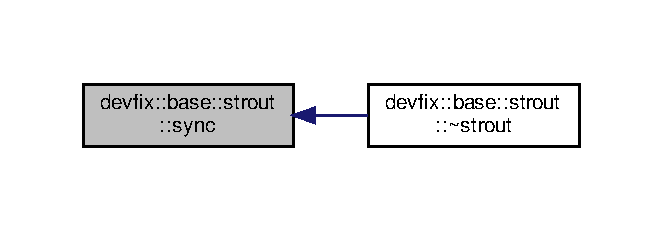
\includegraphics[width=318pt]{structdevfix_1_1base_1_1strout_a50b305dcf9905bfe75fa1bba42718169_icgraph}
\end{center}
\end{figure}


\subsection{Member Data Documentation}
\mbox{\Hypertarget{structdevfix_1_1base_1_1strout_a0625f5cbd10441a4613bf3aae5ab15a1}\label{structdevfix_1_1base_1_1strout_a0625f5cbd10441a4613bf3aae5ab15a1}} 
\index{devfix\+::base\+::strout@{devfix\+::base\+::strout}!buffer\+\_\+@{buffer\+\_\+}}
\index{buffer\+\_\+@{buffer\+\_\+}!devfix\+::base\+::strout@{devfix\+::base\+::strout}}
\subsubsection{\texorpdfstring{buffer\+\_\+}{buffer\_}}
{\footnotesize\ttfamily template$<$class CharT, class Traits = std\+::char\+\_\+traits$<$\+Char\+T$>$, class Allocator = std\+::allocator$<$\+Char\+T$>$$>$ \\
std\+::basic\+\_\+stringstream$<$CharT$>$ \hyperlink{structdevfix_1_1base_1_1strout}{devfix\+::base\+::strout}$<$ CharT, Traits, Allocator $>$\+::buffer\+\_\+\hspace{0.3cm}{\ttfamily [protected]}}

\mbox{\Hypertarget{structdevfix_1_1base_1_1strout_afe9d2f4264b508fd02be4af24dba6bb1}\label{structdevfix_1_1base_1_1strout_afe9d2f4264b508fd02be4af24dba6bb1}} 
\index{devfix\+::base\+::strout@{devfix\+::base\+::strout}!C\+L\+E\+A\+R\+\_\+\+L\+I\+NE@{C\+L\+E\+A\+R\+\_\+\+L\+I\+NE}}
\index{C\+L\+E\+A\+R\+\_\+\+L\+I\+NE@{C\+L\+E\+A\+R\+\_\+\+L\+I\+NE}!devfix\+::base\+::strout@{devfix\+::base\+::strout}}
\subsubsection{\texorpdfstring{C\+L\+E\+A\+R\+\_\+\+L\+I\+NE}{CLEAR\_LINE}}
{\footnotesize\ttfamily template$<$class CharT, class Traits = std\+::char\+\_\+traits$<$\+Char\+T$>$, class Allocator = std\+::allocator$<$\+Char\+T$>$$>$ \\
constexpr std\+::basic\+\_\+string\+\_\+view$<$CharT$>$ \hyperlink{structdevfix_1_1base_1_1strout}{devfix\+::base\+::strout}$<$ CharT, Traits, Allocator $>$\+::C\+L\+E\+A\+R\+\_\+\+L\+I\+NE = \hyperlink{strutil_8h_a72f64e8a28f366adf3cad6c109082271}{M\+U\+L\+T\+I\+S\+T\+R\+I\+NG}(CharT, \char`\"{}\textbackslash{}033\mbox{[}2\+K\textbackslash{}r\char`\"{})\hspace{0.3cm}{\ttfamily [static]}, {\ttfamily [protected]}}

\mbox{\Hypertarget{structdevfix_1_1base_1_1strout_a813fc6630d6565cf5a00e620b536671c}\label{structdevfix_1_1base_1_1strout_a813fc6630d6565cf5a00e620b536671c}} 
\index{devfix\+::base\+::strout@{devfix\+::base\+::strout}!enabled\+\_\+@{enabled\+\_\+}}
\index{enabled\+\_\+@{enabled\+\_\+}!devfix\+::base\+::strout@{devfix\+::base\+::strout}}
\subsubsection{\texorpdfstring{enabled\+\_\+}{enabled\_}}
{\footnotesize\ttfamily template$<$class CharT, class Traits = std\+::char\+\_\+traits$<$\+Char\+T$>$, class Allocator = std\+::allocator$<$\+Char\+T$>$$>$ \\
bool \hyperlink{structdevfix_1_1base_1_1strout}{devfix\+::base\+::strout}$<$ CharT, Traits, Allocator $>$\+::enabled\+\_\+ = true\hspace{0.3cm}{\ttfamily [protected]}}

\mbox{\Hypertarget{structdevfix_1_1base_1_1strout_aa92f98e253e448a0ea897760764486e7}\label{structdevfix_1_1base_1_1strout_aa92f98e253e448a0ea897760764486e7}} 
\index{devfix\+::base\+::strout@{devfix\+::base\+::strout}!pipes\+\_\+@{pipes\+\_\+}}
\index{pipes\+\_\+@{pipes\+\_\+}!devfix\+::base\+::strout@{devfix\+::base\+::strout}}
\subsubsection{\texorpdfstring{pipes\+\_\+}{pipes\_}}
{\footnotesize\ttfamily template$<$class CharT, class Traits = std\+::char\+\_\+traits$<$\+Char\+T$>$, class Allocator = std\+::allocator$<$\+Char\+T$>$$>$ \\
std\+::vector$<$std\+::variant$<$\hyperlink{structdevfix_1_1base_1_1strout_a158aadfad348eeac7c56a8b43699a4d3}{stream\+\_\+t}$\ast$, \hyperlink{structdevfix_1_1base_1_1strout_a2212cb8a99abec10490e891cc67820bb}{pair\+\_\+t}$>$ $>$ \hyperlink{structdevfix_1_1base_1_1strout}{devfix\+::base\+::strout}$<$ CharT, Traits, Allocator $>$\+::pipes\+\_\+\hspace{0.3cm}{\ttfamily [protected]}}

\mbox{\Hypertarget{structdevfix_1_1base_1_1strout_a664c76563ab0f7f0625779aaf0c56395}\label{structdevfix_1_1base_1_1strout_a664c76563ab0f7f0625779aaf0c56395}} 
\index{devfix\+::base\+::strout@{devfix\+::base\+::strout}!prefix\+\_\+@{prefix\+\_\+}}
\index{prefix\+\_\+@{prefix\+\_\+}!devfix\+::base\+::strout@{devfix\+::base\+::strout}}
\subsubsection{\texorpdfstring{prefix\+\_\+}{prefix\_}}
{\footnotesize\ttfamily template$<$class CharT, class Traits = std\+::char\+\_\+traits$<$\+Char\+T$>$, class Allocator = std\+::allocator$<$\+Char\+T$>$$>$ \\
std\+::basic\+\_\+string$<$CharT$>$ \hyperlink{structdevfix_1_1base_1_1strout}{devfix\+::base\+::strout}$<$ CharT, Traits, Allocator $>$\+::prefix\+\_\+\hspace{0.3cm}{\ttfamily [protected]}}

\mbox{\Hypertarget{structdevfix_1_1base_1_1strout_a1e56005b02772de34fddd5e4f44741c3}\label{structdevfix_1_1base_1_1strout_a1e56005b02772de34fddd5e4f44741c3}} 
\index{devfix\+::base\+::strout@{devfix\+::base\+::strout}!prefixed\+\_\+@{prefixed\+\_\+}}
\index{prefixed\+\_\+@{prefixed\+\_\+}!devfix\+::base\+::strout@{devfix\+::base\+::strout}}
\subsubsection{\texorpdfstring{prefixed\+\_\+}{prefixed\_}}
{\footnotesize\ttfamily template$<$class CharT, class Traits = std\+::char\+\_\+traits$<$\+Char\+T$>$, class Allocator = std\+::allocator$<$\+Char\+T$>$$>$ \\
bool \hyperlink{structdevfix_1_1base_1_1strout}{devfix\+::base\+::strout}$<$ CharT, Traits, Allocator $>$\+::prefixed\+\_\+ = true\hspace{0.3cm}{\ttfamily [protected]}}

\mbox{\Hypertarget{structdevfix_1_1base_1_1strout_a76183010a1d8e9360e34b9cd9ab33f7d}\label{structdevfix_1_1base_1_1strout_a76183010a1d8e9360e34b9cd9ab33f7d}} 
\index{devfix\+::base\+::strout@{devfix\+::base\+::strout}!S\+TX@{S\+TX}}
\index{S\+TX@{S\+TX}!devfix\+::base\+::strout@{devfix\+::base\+::strout}}
\subsubsection{\texorpdfstring{S\+TX}{STX}}
{\footnotesize\ttfamily template$<$class CharT, class Traits = std\+::char\+\_\+traits$<$\+Char\+T$>$, class Allocator = std\+::allocator$<$\+Char\+T$>$$>$ \\
constexpr CharT \hyperlink{structdevfix_1_1base_1_1strout}{devfix\+::base\+::strout}$<$ CharT, Traits, Allocator $>$\+::S\+TX = static\+\_\+cast$<$CharT$>$(\textquotesingle{}\textbackslash{}x02\textquotesingle{})\hspace{0.3cm}{\ttfamily [static]}}



Start of Text, clear whole line before new text gets displayed. 



The documentation for this struct was generated from the following file\+:\begin{DoxyCompactItemize}
\item 
devfix/base/\hyperlink{strout_8h}{strout.\+h}\end{DoxyCompactItemize}

\hypertarget{structdevfix_1_1base_1_1strutil}{}\section{devfix\+:\+:base\+:\+:strutil Struct Reference}
\label{structdevfix_1_1base_1_1strutil}\index{devfix\+::base\+::strutil@{devfix\+::base\+::strutil}}


{\ttfamily \#include $<$strutil.\+h$>$}



The documentation for this struct was generated from the following file\+:\begin{DoxyCompactItemize}
\item 
devfix/base/\hyperlink{strutil_8h}{strutil.\+h}\end{DoxyCompactItemize}

\hypertarget{structdevfix_1_1base_1_1__math_1_1Table}{}\section{devfix\+:\+:base\+:\+:\+\_\+math\+:\+:Table$<$ T, N, G, Args $>$ Struct Template Reference}
\label{structdevfix_1_1base_1_1__math_1_1Table}\index{devfix\+::base\+::\+\_\+math\+::\+Table$<$ T, N, G, Args $>$@{devfix\+::base\+::\+\_\+math\+::\+Table$<$ T, N, G, Args $>$}}


{\ttfamily \#include $<$math.\+h$>$}

\subsection*{Public Member Functions}
\begin{DoxyCompactItemize}
\item 
constexpr \hyperlink{structdevfix_1_1base_1_1__math_1_1Table_acc5b398c45b9dcd7846f5228611a43b9}{Table} (G gen, Args ... args)
\end{DoxyCompactItemize}
\subsection*{Public Attributes}
\begin{DoxyCompactItemize}
\item 
T \hyperlink{structdevfix_1_1base_1_1__math_1_1Table_a3352fdb7ab931816a7d131b643099c97}{values} \mbox{[}N\mbox{]}
\end{DoxyCompactItemize}


\subsection{Constructor \& Destructor Documentation}
\mbox{\Hypertarget{structdevfix_1_1base_1_1__math_1_1Table_acc5b398c45b9dcd7846f5228611a43b9}\label{structdevfix_1_1base_1_1__math_1_1Table_acc5b398c45b9dcd7846f5228611a43b9}} 
\index{devfix\+::base\+::\+\_\+math\+::\+Table@{devfix\+::base\+::\+\_\+math\+::\+Table}!Table@{Table}}
\index{Table@{Table}!devfix\+::base\+::\+\_\+math\+::\+Table@{devfix\+::base\+::\+\_\+math\+::\+Table}}
\subsubsection{\texorpdfstring{Table()}{Table()}}
{\footnotesize\ttfamily template$<$typename T , std\+::size\+\_\+t N, typename G , typename ... Args$>$ \\
constexpr \hyperlink{structdevfix_1_1base_1_1__math_1_1Table}{devfix\+::base\+::\+\_\+math\+::\+Table}$<$ T, N, G, Args $>$\+::\hyperlink{structdevfix_1_1base_1_1__math_1_1Table}{Table} (\begin{DoxyParamCaption}\item[{G}]{gen,  }\item[{Args ...}]{args }\end{DoxyParamCaption})\hspace{0.3cm}{\ttfamily [inline]}}



\subsection{Member Data Documentation}
\mbox{\Hypertarget{structdevfix_1_1base_1_1__math_1_1Table_a3352fdb7ab931816a7d131b643099c97}\label{structdevfix_1_1base_1_1__math_1_1Table_a3352fdb7ab931816a7d131b643099c97}} 
\index{devfix\+::base\+::\+\_\+math\+::\+Table@{devfix\+::base\+::\+\_\+math\+::\+Table}!values@{values}}
\index{values@{values}!devfix\+::base\+::\+\_\+math\+::\+Table@{devfix\+::base\+::\+\_\+math\+::\+Table}}
\subsubsection{\texorpdfstring{values}{values}}
{\footnotesize\ttfamily template$<$typename T , std\+::size\+\_\+t N, typename G , typename ... Args$>$ \\
T \hyperlink{structdevfix_1_1base_1_1__math_1_1Table}{devfix\+::base\+::\+\_\+math\+::\+Table}$<$ T, N, G, Args $>$\+::values\mbox{[}N\mbox{]}}



The documentation for this struct was generated from the following file\+:\begin{DoxyCompactItemize}
\item 
devfix/base/\hyperlink{math_8h}{math.\+h}\end{DoxyCompactItemize}

\hypertarget{structdevfix_1_1base_1_1time}{}\section{devfix\+:\+:base\+:\+:time Struct Reference}
\label{structdevfix_1_1base_1_1time}\index{devfix\+::base\+::time@{devfix\+::base\+::time}}


{\ttfamily \#include $<$time.\+h$>$}

\subsection*{Static Public Member Functions}
\begin{DoxyCompactItemize}
\item 
static \hyperlink{structdevfix_1_1base_1_1time}{time} \hyperlink{structdevfix_1_1base_1_1time_a14d0b48fe09bf355aa64f3a5e2c60418}{get\+\_\+tm} (std\+::tm $\ast$tm)
\end{DoxyCompactItemize}
\subsection*{Public Attributes}
\begin{DoxyCompactItemize}
\item 
int \hyperlink{structdevfix_1_1base_1_1time_a7a39795f67f0e3f1bea48cc790ef0bdb}{second}
\item 
int \hyperlink{structdevfix_1_1base_1_1time_a2e36d9cbccf1144093e09674d4d9db24}{minute}
\item 
int \hyperlink{structdevfix_1_1base_1_1time_a82a691ea0cc8b65beac2e3d3b4254c55}{hour}
\item 
int \hyperlink{structdevfix_1_1base_1_1time_ae5a080003e7020960c31e47cf30a21ba}{day}
\item 
int \hyperlink{structdevfix_1_1base_1_1time_a781a7e9d96a916305e1a9e2c261c1a0f}{month}
\item 
int \hyperlink{structdevfix_1_1base_1_1time_a28e7dfbcd21ff6c915f66497b86168d9}{year}
\end{DoxyCompactItemize}


\subsection{Member Function Documentation}
\mbox{\Hypertarget{structdevfix_1_1base_1_1time_a14d0b48fe09bf355aa64f3a5e2c60418}\label{structdevfix_1_1base_1_1time_a14d0b48fe09bf355aa64f3a5e2c60418}} 
\index{devfix\+::base\+::time@{devfix\+::base\+::time}!get\+\_\+tm@{get\+\_\+tm}}
\index{get\+\_\+tm@{get\+\_\+tm}!devfix\+::base\+::time@{devfix\+::base\+::time}}
\subsubsection{\texorpdfstring{get\+\_\+tm()}{get\_tm()}}
{\footnotesize\ttfamily static \hyperlink{structdevfix_1_1base_1_1time}{time} devfix\+::base\+::time\+::get\+\_\+tm (\begin{DoxyParamCaption}\item[{std\+::tm $\ast$}]{tm }\end{DoxyParamCaption})\hspace{0.3cm}{\ttfamily [inline]}, {\ttfamily [static]}}



\subsection{Member Data Documentation}
\mbox{\Hypertarget{structdevfix_1_1base_1_1time_ae5a080003e7020960c31e47cf30a21ba}\label{structdevfix_1_1base_1_1time_ae5a080003e7020960c31e47cf30a21ba}} 
\index{devfix\+::base\+::time@{devfix\+::base\+::time}!day@{day}}
\index{day@{day}!devfix\+::base\+::time@{devfix\+::base\+::time}}
\subsubsection{\texorpdfstring{day}{day}}
{\footnotesize\ttfamily int devfix\+::base\+::time\+::day}

\mbox{\Hypertarget{structdevfix_1_1base_1_1time_a82a691ea0cc8b65beac2e3d3b4254c55}\label{structdevfix_1_1base_1_1time_a82a691ea0cc8b65beac2e3d3b4254c55}} 
\index{devfix\+::base\+::time@{devfix\+::base\+::time}!hour@{hour}}
\index{hour@{hour}!devfix\+::base\+::time@{devfix\+::base\+::time}}
\subsubsection{\texorpdfstring{hour}{hour}}
{\footnotesize\ttfamily int devfix\+::base\+::time\+::hour}

\mbox{\Hypertarget{structdevfix_1_1base_1_1time_a2e36d9cbccf1144093e09674d4d9db24}\label{structdevfix_1_1base_1_1time_a2e36d9cbccf1144093e09674d4d9db24}} 
\index{devfix\+::base\+::time@{devfix\+::base\+::time}!minute@{minute}}
\index{minute@{minute}!devfix\+::base\+::time@{devfix\+::base\+::time}}
\subsubsection{\texorpdfstring{minute}{minute}}
{\footnotesize\ttfamily int devfix\+::base\+::time\+::minute}

\mbox{\Hypertarget{structdevfix_1_1base_1_1time_a781a7e9d96a916305e1a9e2c261c1a0f}\label{structdevfix_1_1base_1_1time_a781a7e9d96a916305e1a9e2c261c1a0f}} 
\index{devfix\+::base\+::time@{devfix\+::base\+::time}!month@{month}}
\index{month@{month}!devfix\+::base\+::time@{devfix\+::base\+::time}}
\subsubsection{\texorpdfstring{month}{month}}
{\footnotesize\ttfamily int devfix\+::base\+::time\+::month}

\mbox{\Hypertarget{structdevfix_1_1base_1_1time_a7a39795f67f0e3f1bea48cc790ef0bdb}\label{structdevfix_1_1base_1_1time_a7a39795f67f0e3f1bea48cc790ef0bdb}} 
\index{devfix\+::base\+::time@{devfix\+::base\+::time}!second@{second}}
\index{second@{second}!devfix\+::base\+::time@{devfix\+::base\+::time}}
\subsubsection{\texorpdfstring{second}{second}}
{\footnotesize\ttfamily int devfix\+::base\+::time\+::second}

\mbox{\Hypertarget{structdevfix_1_1base_1_1time_a28e7dfbcd21ff6c915f66497b86168d9}\label{structdevfix_1_1base_1_1time_a28e7dfbcd21ff6c915f66497b86168d9}} 
\index{devfix\+::base\+::time@{devfix\+::base\+::time}!year@{year}}
\index{year@{year}!devfix\+::base\+::time@{devfix\+::base\+::time}}
\subsubsection{\texorpdfstring{year}{year}}
{\footnotesize\ttfamily int devfix\+::base\+::time\+::year}



The documentation for this struct was generated from the following file\+:\begin{DoxyCompactItemize}
\item 
devfix/base/\hyperlink{time_8h}{time.\+h}\end{DoxyCompactItemize}

\hypertarget{structdevfix_1_1base_1_1error_1_1timeoutexception}{}\section{devfix\+:\+:base\+:\+:error\+:\+:timeoutexception Struct Reference}
\label{structdevfix_1_1base_1_1error_1_1timeoutexception}\index{devfix\+::base\+::error\+::timeoutexception@{devfix\+::base\+::error\+::timeoutexception}}


Exception thrown when a blocking operation times out.  




{\ttfamily \#include $<$timeoutexception.\+h$>$}



Inheritance diagram for devfix\+:\+:base\+:\+:error\+:\+:timeoutexception\+:
\nopagebreak
\begin{figure}[H]
\begin{center}
\leavevmode
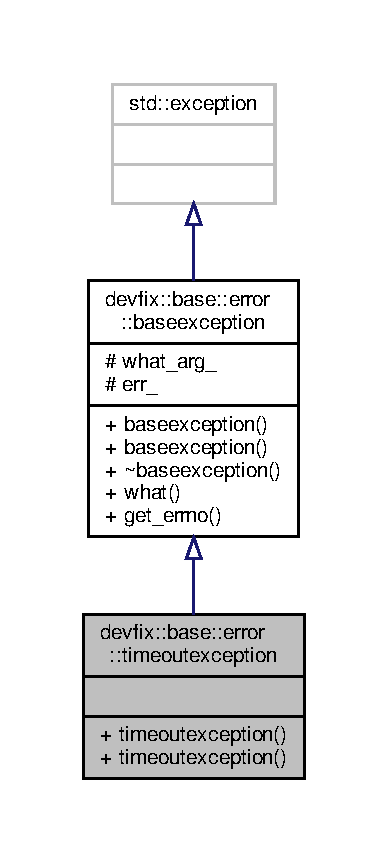
\includegraphics[width=186pt]{structdevfix_1_1base_1_1error_1_1timeoutexception__inherit__graph}
\end{center}
\end{figure}
\subsection*{Public Member Functions}
\begin{DoxyCompactItemize}
\item 
\hyperlink{structdevfix_1_1base_1_1error_1_1timeoutexception_a1795157a577b45e026b11c3b3cec80b3}{timeoutexception} (const std\+::string \&what\+\_\+arg, int err=0)
\item 
\hyperlink{structdevfix_1_1base_1_1error_1_1timeoutexception_ac35d347533a4a8ba1d19900846784e72}{timeoutexception} (const char $\ast$what\+\_\+arg, int err=0)
\end{DoxyCompactItemize}
\subsection*{Additional Inherited Members}


\subsection{Detailed Description}
Exception thrown when a blocking operation times out. 

Blocking operations for which a timeout is specified need a means to indicate that the timeout has occurred. For many such operations it is possible to return a value that indicates timeout; when that is not possible or desirable then Timeout\+Exception should be declared and thrown. 

\subsection{Constructor \& Destructor Documentation}
\mbox{\Hypertarget{structdevfix_1_1base_1_1error_1_1timeoutexception_a1795157a577b45e026b11c3b3cec80b3}\label{structdevfix_1_1base_1_1error_1_1timeoutexception_a1795157a577b45e026b11c3b3cec80b3}} 
\index{devfix\+::base\+::error\+::timeoutexception@{devfix\+::base\+::error\+::timeoutexception}!timeoutexception@{timeoutexception}}
\index{timeoutexception@{timeoutexception}!devfix\+::base\+::error\+::timeoutexception@{devfix\+::base\+::error\+::timeoutexception}}
\subsubsection{\texorpdfstring{timeoutexception()}{timeoutexception()}\hspace{0.1cm}{\footnotesize\ttfamily [1/2]}}
{\footnotesize\ttfamily devfix\+::base\+::error\+::timeoutexception\+::timeoutexception (\begin{DoxyParamCaption}\item[{const std\+::string \&}]{what\+\_\+arg,  }\item[{int}]{err = {\ttfamily 0} }\end{DoxyParamCaption})\hspace{0.3cm}{\ttfamily [inline]}, {\ttfamily [explicit]}}

Constructs the error object with what\+\_\+arg as explanatory string that can be accessed through \hyperlink{structdevfix_1_1base_1_1error_1_1baseexception_a16327152a55d65b1e537825231fbd452}{what()}. 
\begin{DoxyParams}{Parameters}
{\em what\+\_\+arg} & explanatory std\+::string \\
\hline
{\em err} & c error code (errno) \\
\hline
\end{DoxyParams}
\mbox{\Hypertarget{structdevfix_1_1base_1_1error_1_1timeoutexception_ac35d347533a4a8ba1d19900846784e72}\label{structdevfix_1_1base_1_1error_1_1timeoutexception_ac35d347533a4a8ba1d19900846784e72}} 
\index{devfix\+::base\+::error\+::timeoutexception@{devfix\+::base\+::error\+::timeoutexception}!timeoutexception@{timeoutexception}}
\index{timeoutexception@{timeoutexception}!devfix\+::base\+::error\+::timeoutexception@{devfix\+::base\+::error\+::timeoutexception}}
\subsubsection{\texorpdfstring{timeoutexception()}{timeoutexception()}\hspace{0.1cm}{\footnotesize\ttfamily [2/2]}}
{\footnotesize\ttfamily devfix\+::base\+::error\+::timeoutexception\+::timeoutexception (\begin{DoxyParamCaption}\item[{const char $\ast$}]{what\+\_\+arg,  }\item[{int}]{err = {\ttfamily 0} }\end{DoxyParamCaption})\hspace{0.3cm}{\ttfamily [inline]}, {\ttfamily [explicit]}}

Constructs the error object with what\+\_\+arg as explanatory string that can be accessed through \hyperlink{structdevfix_1_1base_1_1error_1_1baseexception_a16327152a55d65b1e537825231fbd452}{what()}. 
\begin{DoxyParams}{Parameters}
{\em what\+\_\+arg} & explanatory c-\/string \\
\hline
{\em err} & c error code (errno) \\
\hline
\end{DoxyParams}


The documentation for this struct was generated from the following file\+:\begin{DoxyCompactItemize}
\item 
devfix/base/error/\hyperlink{timeoutexception_8h}{timeoutexception.\+h}\end{DoxyCompactItemize}

\hypertarget{structdevfix_1_1dsp_1_1window}{}\section{devfix\+:\+:dsp\+:\+:window$<$ FloatT $>$ Struct Template Reference}
\label{structdevfix_1_1dsp_1_1window}\index{devfix\+::dsp\+::window$<$ Float\+T $>$@{devfix\+::dsp\+::window$<$ Float\+T $>$}}


buffer for the values of window function for a specific window length  




{\ttfamily \#include $<$window.\+h$>$}

\subsection*{Public Member Functions}
\begin{DoxyCompactItemize}
\item 
\hyperlink{structdevfix_1_1dsp_1_1window_a9a95322d9d9547f393e528cdfe3ec2aa}{window} (\hyperlink{namespacedevfix_1_1dsp_a6667d1bec03c0d82f87521b87d3fcf24}{winfun\+\_\+t}$<$ FloatT $>$ function, std\+::size\+\_\+t \hyperlink{structdevfix_1_1dsp_1_1window_a24610f1f5682113df6e949575517d171}{size}, bool correct\+\_\+gain=true)
\begin{DoxyCompactList}\small\item\em create new window and calculate all its values using a window function \end{DoxyCompactList}\item 
std\+::size\+\_\+t \hyperlink{structdevfix_1_1dsp_1_1window_a24610f1f5682113df6e949575517d171}{size} () const
\item 
void \hyperlink{structdevfix_1_1dsp_1_1window_aebc5f8902372df2cb349e009660f6752}{apply} (FloatT $\ast$field) const
\begin{DoxyCompactList}\small\item\em multiplies each real field element with the window value at the same index, the length of the field has to be the same as the window size \end{DoxyCompactList}\item 
void \hyperlink{structdevfix_1_1dsp_1_1window_ac048886c4ae01a95d5272cbf73eac542}{apply} (std\+::vector$<$ FloatT $>$ \&vec) const
\begin{DoxyCompactList}\small\item\em multiplies each real vector element with the window value at the same index, the length of the vector has to be the same as the window size \end{DoxyCompactList}\item 
{\footnotesize template$<$std\+::size\+\_\+t N$>$ }\\void \hyperlink{structdevfix_1_1dsp_1_1window_a3c9dc67499f51b6a70657fd71be5faa3}{apply} (std\+::array$<$ FloatT, N $>$ \&arr)
\begin{DoxyCompactList}\small\item\em multiplies each real array element with the window value at the same index, the length of the array has to be the same as the window size \end{DoxyCompactList}\item 
void \hyperlink{structdevfix_1_1dsp_1_1window_a8c378c67016543fe7d69bf84145994e6}{apply} (std\+::complex$<$ FloatT $>$ $\ast$field) const
\begin{DoxyCompactList}\small\item\em multiplies each complex field element with the window value at the same index, the length of the field has to be the same as the window size \end{DoxyCompactList}\item 
void \hyperlink{structdevfix_1_1dsp_1_1window_a7d9fb193d2286f50aabc2ea0243a5465}{apply} (std\+::vector$<$ std\+::complex$<$ FloatT $>$$>$ \&vec) const
\begin{DoxyCompactList}\small\item\em multiplies each complex vector element with the window value at the same index, the length of the vector has to be the same as the window size \end{DoxyCompactList}\item 
{\footnotesize template$<$std\+::size\+\_\+t N$>$ }\\void \hyperlink{structdevfix_1_1dsp_1_1window_a3b101f8761a003d0bdbd90c6f1de2183}{apply} (std\+::array$<$ std\+::complex$<$ FloatT $>$, N $>$ \&arr)
\begin{DoxyCompactList}\small\item\em multiplies each complex array element with the window value at the same index, the length of the array has to be the same as the window size \end{DoxyCompactList}\end{DoxyCompactItemize}


\subsection{Detailed Description}
\subsubsection*{template$<$typename FloatT$>$\newline
struct devfix\+::dsp\+::window$<$ Float\+T $>$}

buffer for the values of window function for a specific window length 


\begin{DoxyTemplParams}{Template Parameters}
{\em FloatT} & type of floating point numbers \\
\hline
\end{DoxyTemplParams}


\subsection{Constructor \& Destructor Documentation}
\mbox{\Hypertarget{structdevfix_1_1dsp_1_1window_a9a95322d9d9547f393e528cdfe3ec2aa}\label{structdevfix_1_1dsp_1_1window_a9a95322d9d9547f393e528cdfe3ec2aa}} 
\index{devfix\+::dsp\+::window@{devfix\+::dsp\+::window}!window@{window}}
\index{window@{window}!devfix\+::dsp\+::window@{devfix\+::dsp\+::window}}
\subsubsection{\texorpdfstring{window()}{window()}}
{\footnotesize\ttfamily template$<$typename FloatT$>$ \\
\hyperlink{structdevfix_1_1dsp_1_1window}{devfix\+::dsp\+::window}$<$ FloatT $>$\+::\hyperlink{structdevfix_1_1dsp_1_1window}{window} (\begin{DoxyParamCaption}\item[{\hyperlink{namespacedevfix_1_1dsp_a6667d1bec03c0d82f87521b87d3fcf24}{winfun\+\_\+t}$<$ FloatT $>$}]{function,  }\item[{std\+::size\+\_\+t}]{size,  }\item[{bool}]{correct\+\_\+gain = {\ttfamily true} }\end{DoxyParamCaption})\hspace{0.3cm}{\ttfamily [inline]}}



create new window and calculate all its values using a window function 


\begin{DoxyParams}{Parameters}
{\em function} & window function to calculate the window values with \\
\hline
{\em size} & window size, count of values \\
\hline
{\em correct\+\_\+gain} & if true, calculates the window\textquotesingle{}s gain and multiplies each window value with it \\
\hline
\end{DoxyParams}


\subsection{Member Function Documentation}
\mbox{\Hypertarget{structdevfix_1_1dsp_1_1window_aebc5f8902372df2cb349e009660f6752}\label{structdevfix_1_1dsp_1_1window_aebc5f8902372df2cb349e009660f6752}} 
\index{devfix\+::dsp\+::window@{devfix\+::dsp\+::window}!apply@{apply}}
\index{apply@{apply}!devfix\+::dsp\+::window@{devfix\+::dsp\+::window}}
\subsubsection{\texorpdfstring{apply()}{apply()}\hspace{0.1cm}{\footnotesize\ttfamily [1/6]}}
{\footnotesize\ttfamily template$<$typename FloatT$>$ \\
void \hyperlink{structdevfix_1_1dsp_1_1window}{devfix\+::dsp\+::window}$<$ FloatT $>$\+::apply (\begin{DoxyParamCaption}\item[{FloatT $\ast$}]{field }\end{DoxyParamCaption}) const\hspace{0.3cm}{\ttfamily [inline]}}



multiplies each real field element with the window value at the same index, the length of the field has to be the same as the window size 


\begin{DoxyParams}{Parameters}
{\em field} & input field of real numbers \\
\hline
\end{DoxyParams}
Here is the caller graph for this function\+:
\nopagebreak
\begin{figure}[H]
\begin{center}
\leavevmode
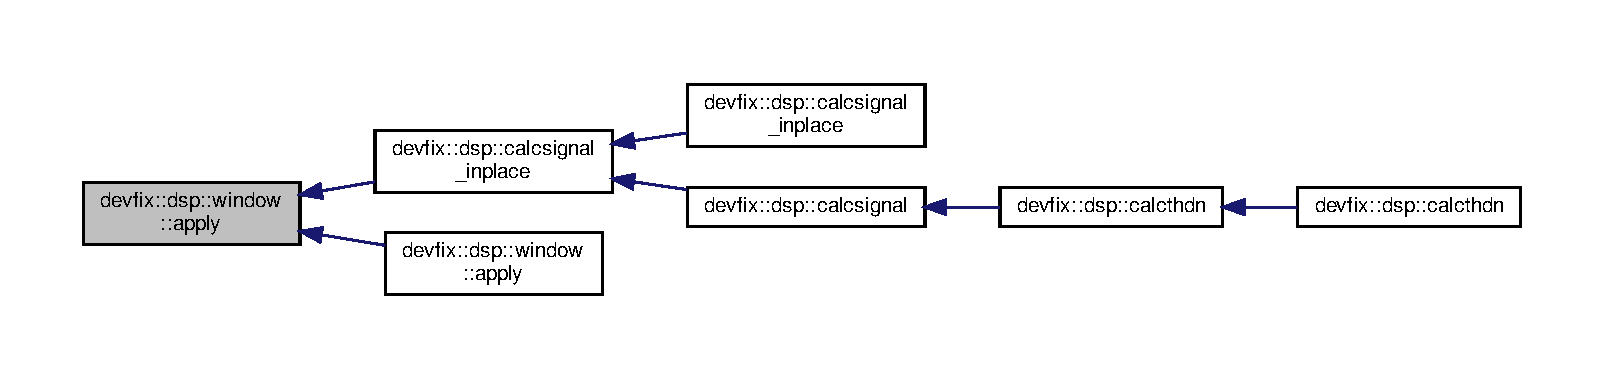
\includegraphics[width=350pt]{structdevfix_1_1dsp_1_1window_aebc5f8902372df2cb349e009660f6752_icgraph}
\end{center}
\end{figure}
\mbox{\Hypertarget{structdevfix_1_1dsp_1_1window_ac048886c4ae01a95d5272cbf73eac542}\label{structdevfix_1_1dsp_1_1window_ac048886c4ae01a95d5272cbf73eac542}} 
\index{devfix\+::dsp\+::window@{devfix\+::dsp\+::window}!apply@{apply}}
\index{apply@{apply}!devfix\+::dsp\+::window@{devfix\+::dsp\+::window}}
\subsubsection{\texorpdfstring{apply()}{apply()}\hspace{0.1cm}{\footnotesize\ttfamily [2/6]}}
{\footnotesize\ttfamily template$<$typename FloatT$>$ \\
void \hyperlink{structdevfix_1_1dsp_1_1window}{devfix\+::dsp\+::window}$<$ FloatT $>$\+::apply (\begin{DoxyParamCaption}\item[{std\+::vector$<$ FloatT $>$ \&}]{vec }\end{DoxyParamCaption}) const\hspace{0.3cm}{\ttfamily [inline]}}



multiplies each real vector element with the window value at the same index, the length of the vector has to be the same as the window size 


\begin{DoxyParams}{Parameters}
{\em vec} & input vector of real numbers \\
\hline
\end{DoxyParams}
\mbox{\Hypertarget{structdevfix_1_1dsp_1_1window_a3c9dc67499f51b6a70657fd71be5faa3}\label{structdevfix_1_1dsp_1_1window_a3c9dc67499f51b6a70657fd71be5faa3}} 
\index{devfix\+::dsp\+::window@{devfix\+::dsp\+::window}!apply@{apply}}
\index{apply@{apply}!devfix\+::dsp\+::window@{devfix\+::dsp\+::window}}
\subsubsection{\texorpdfstring{apply()}{apply()}\hspace{0.1cm}{\footnotesize\ttfamily [3/6]}}
{\footnotesize\ttfamily template$<$typename FloatT$>$ \\
template$<$std\+::size\+\_\+t N$>$ \\
void \hyperlink{structdevfix_1_1dsp_1_1window}{devfix\+::dsp\+::window}$<$ FloatT $>$\+::apply (\begin{DoxyParamCaption}\item[{std\+::array$<$ FloatT, N $>$ \&}]{arr }\end{DoxyParamCaption})\hspace{0.3cm}{\ttfamily [inline]}}



multiplies each real array element with the window value at the same index, the length of the array has to be the same as the window size 


\begin{DoxyTemplParams}{Template Parameters}
{\em N} & array length \\
\hline
\end{DoxyTemplParams}

\begin{DoxyParams}{Parameters}
{\em arr} & input array of real numbers \\
\hline
\end{DoxyParams}
\mbox{\Hypertarget{structdevfix_1_1dsp_1_1window_a8c378c67016543fe7d69bf84145994e6}\label{structdevfix_1_1dsp_1_1window_a8c378c67016543fe7d69bf84145994e6}} 
\index{devfix\+::dsp\+::window@{devfix\+::dsp\+::window}!apply@{apply}}
\index{apply@{apply}!devfix\+::dsp\+::window@{devfix\+::dsp\+::window}}
\subsubsection{\texorpdfstring{apply()}{apply()}\hspace{0.1cm}{\footnotesize\ttfamily [4/6]}}
{\footnotesize\ttfamily template$<$typename FloatT$>$ \\
void \hyperlink{structdevfix_1_1dsp_1_1window}{devfix\+::dsp\+::window}$<$ FloatT $>$\+::apply (\begin{DoxyParamCaption}\item[{std\+::complex$<$ FloatT $>$ $\ast$}]{field }\end{DoxyParamCaption}) const\hspace{0.3cm}{\ttfamily [inline]}}



multiplies each complex field element with the window value at the same index, the length of the field has to be the same as the window size 


\begin{DoxyParams}{Parameters}
{\em field} & input field of complex numbers \\
\hline
\end{DoxyParams}
\mbox{\Hypertarget{structdevfix_1_1dsp_1_1window_a7d9fb193d2286f50aabc2ea0243a5465}\label{structdevfix_1_1dsp_1_1window_a7d9fb193d2286f50aabc2ea0243a5465}} 
\index{devfix\+::dsp\+::window@{devfix\+::dsp\+::window}!apply@{apply}}
\index{apply@{apply}!devfix\+::dsp\+::window@{devfix\+::dsp\+::window}}
\subsubsection{\texorpdfstring{apply()}{apply()}\hspace{0.1cm}{\footnotesize\ttfamily [5/6]}}
{\footnotesize\ttfamily template$<$typename FloatT$>$ \\
void \hyperlink{structdevfix_1_1dsp_1_1window}{devfix\+::dsp\+::window}$<$ FloatT $>$\+::apply (\begin{DoxyParamCaption}\item[{std\+::vector$<$ std\+::complex$<$ FloatT $>$$>$ \&}]{vec }\end{DoxyParamCaption}) const\hspace{0.3cm}{\ttfamily [inline]}}



multiplies each complex vector element with the window value at the same index, the length of the vector has to be the same as the window size 


\begin{DoxyParams}{Parameters}
{\em vec} & input vector of complex numbers \\
\hline
\end{DoxyParams}
\mbox{\Hypertarget{structdevfix_1_1dsp_1_1window_a3b101f8761a003d0bdbd90c6f1de2183}\label{structdevfix_1_1dsp_1_1window_a3b101f8761a003d0bdbd90c6f1de2183}} 
\index{devfix\+::dsp\+::window@{devfix\+::dsp\+::window}!apply@{apply}}
\index{apply@{apply}!devfix\+::dsp\+::window@{devfix\+::dsp\+::window}}
\subsubsection{\texorpdfstring{apply()}{apply()}\hspace{0.1cm}{\footnotesize\ttfamily [6/6]}}
{\footnotesize\ttfamily template$<$typename FloatT$>$ \\
template$<$std\+::size\+\_\+t N$>$ \\
void \hyperlink{structdevfix_1_1dsp_1_1window}{devfix\+::dsp\+::window}$<$ FloatT $>$\+::apply (\begin{DoxyParamCaption}\item[{std\+::array$<$ std\+::complex$<$ FloatT $>$, N $>$ \&}]{arr }\end{DoxyParamCaption})\hspace{0.3cm}{\ttfamily [inline]}}



multiplies each complex array element with the window value at the same index, the length of the array has to be the same as the window size 


\begin{DoxyTemplParams}{Template Parameters}
{\em N} & array length \\
\hline
\end{DoxyTemplParams}

\begin{DoxyParams}{Parameters}
{\em arr} & input array of complex numbers \\
\hline
\end{DoxyParams}
\mbox{\Hypertarget{structdevfix_1_1dsp_1_1window_a24610f1f5682113df6e949575517d171}\label{structdevfix_1_1dsp_1_1window_a24610f1f5682113df6e949575517d171}} 
\index{devfix\+::dsp\+::window@{devfix\+::dsp\+::window}!size@{size}}
\index{size@{size}!devfix\+::dsp\+::window@{devfix\+::dsp\+::window}}
\subsubsection{\texorpdfstring{size()}{size()}}
{\footnotesize\ttfamily template$<$typename FloatT$>$ \\
std\+::size\+\_\+t \hyperlink{structdevfix_1_1dsp_1_1window}{devfix\+::dsp\+::window}$<$ FloatT $>$\+::size (\begin{DoxyParamCaption}{ }\end{DoxyParamCaption}) const\hspace{0.3cm}{\ttfamily [inline]}}

\begin{DoxyReturn}{Returns}
count of window values 
\end{DoxyReturn}


The documentation for this struct was generated from the following file\+:\begin{DoxyCompactItemize}
\item 
devfix/dsp/\hyperlink{window_8h}{window.\+h}\end{DoxyCompactItemize}

\chapter{File Documentation}
\hypertarget{baseexception_8h}{}\section{devfix/base/error/baseexception.h File Reference}
\label{baseexception_8h}\index{devfix/base/error/baseexception.\+h@{devfix/base/error/baseexception.\+h}}
{\ttfamily \#include $<$exception$>$}\newline
{\ttfamily \#include $<$string$>$}\newline
{\ttfamily \#include $<$cstring$>$}\newline
Include dependency graph for baseexception.\+h\+:\nopagebreak
\begin{figure}[H]
\begin{center}
\leavevmode
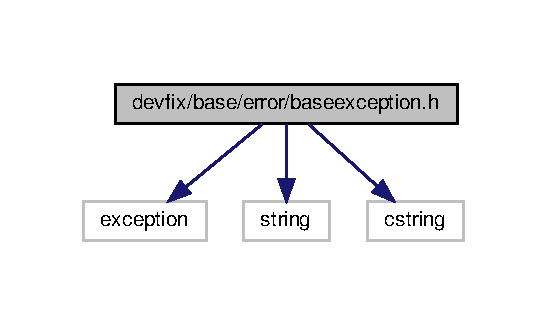
\includegraphics[width=263pt]{baseexception_8h__incl}
\end{center}
\end{figure}
This graph shows which files directly or indirectly include this file\+:\nopagebreak
\begin{figure}[H]
\begin{center}
\leavevmode
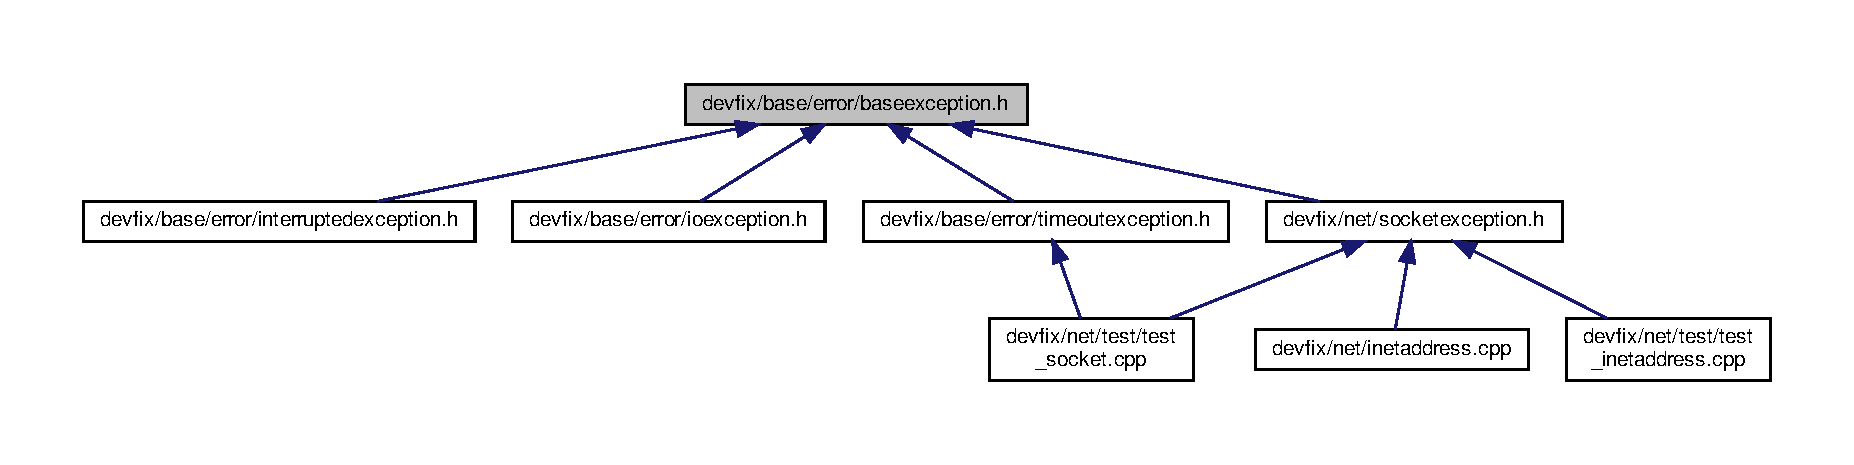
\includegraphics[width=350pt]{baseexception_8h__dep__incl}
\end{center}
\end{figure}
\subsection*{Classes}
\begin{DoxyCompactItemize}
\item 
struct \hyperlink{structdevfix_1_1base_1_1error_1_1baseexception}{devfix\+::base\+::error\+::baseexception}
\begin{DoxyCompactList}\small\item\em Abstract error base class. \end{DoxyCompactList}\end{DoxyCompactItemize}
\subsection*{Namespaces}
\begin{DoxyCompactItemize}
\item 
 \hyperlink{namespacedevfix_1_1base_1_1error}{devfix\+::base\+::error}
\begin{DoxyCompactList}\small\item\em Namespace for general errors like timeouts or io failures. \end{DoxyCompactList}\end{DoxyCompactItemize}
\subsection*{Macros}
\begin{DoxyCompactItemize}
\item 
\#define \hyperlink{baseexception_8h_ad012bfdf381fa2c9100432def38f62ba}{exception\+\_\+guard\+\_\+m}(err,  exception\+\_\+class,  message)
\item 
\#define \hyperlink{baseexception_8h_a0c2a0196acc0ae3484a38b3a3172b016}{exception\+\_\+guard}(err,  exception\+\_\+class)~\hyperlink{baseexception_8h_ad012bfdf381fa2c9100432def38f62ba}{exception\+\_\+guard\+\_\+m}(err, exception\+\_\+class, std\+::strerror(errno))
\end{DoxyCompactItemize}


\subsection{Macro Definition Documentation}
\mbox{\Hypertarget{baseexception_8h_a0c2a0196acc0ae3484a38b3a3172b016}\label{baseexception_8h_a0c2a0196acc0ae3484a38b3a3172b016}} 
\index{baseexception.\+h@{baseexception.\+h}!exception\+\_\+guard@{exception\+\_\+guard}}
\index{exception\+\_\+guard@{exception\+\_\+guard}!baseexception.\+h@{baseexception.\+h}}
\subsubsection{\texorpdfstring{exception\+\_\+guard}{exception\_guard}}
{\footnotesize\ttfamily \#define exception\+\_\+guard(\begin{DoxyParamCaption}\item[{}]{err,  }\item[{}]{exception\+\_\+class }\end{DoxyParamCaption})~\hyperlink{baseexception_8h_ad012bfdf381fa2c9100432def38f62ba}{exception\+\_\+guard\+\_\+m}(err, exception\+\_\+class, std\+::strerror(errno))}

\mbox{\Hypertarget{baseexception_8h_ad012bfdf381fa2c9100432def38f62ba}\label{baseexception_8h_ad012bfdf381fa2c9100432def38f62ba}} 
\index{baseexception.\+h@{baseexception.\+h}!exception\+\_\+guard\+\_\+m@{exception\+\_\+guard\+\_\+m}}
\index{exception\+\_\+guard\+\_\+m@{exception\+\_\+guard\+\_\+m}!baseexception.\+h@{baseexception.\+h}}
\subsubsection{\texorpdfstring{exception\+\_\+guard\+\_\+m}{exception\_guard\_m}}
{\footnotesize\ttfamily \#define exception\+\_\+guard\+\_\+m(\begin{DoxyParamCaption}\item[{}]{err,  }\item[{}]{exception\+\_\+class,  }\item[{}]{message }\end{DoxyParamCaption})}

{\bfseries Value\+:}
\begin{DoxyCode}
\textcolor{keywordflow}{if} (err) \(\backslash\)
    throw exception\_class(message + std::string(\textcolor{stringliteral}{" @ "}) + \hyperlink{platform_8h_acf16e3e245e0e3b5d45b2a11075d4d36}{SOURCE\_LINE}, errno)
\end{DoxyCode}

\hypertarget{interruptedexception_8h}{}\section{devfix/base/error/interruptedexception.h File Reference}
\label{interruptedexception_8h}\index{devfix/base/error/interruptedexception.\+h@{devfix/base/error/interruptedexception.\+h}}
{\ttfamily \#include \char`\"{}baseexception.\+h\char`\"{}}\newline
Include dependency graph for interruptedexception.\+h\+:\nopagebreak
\begin{figure}[H]
\begin{center}
\leavevmode
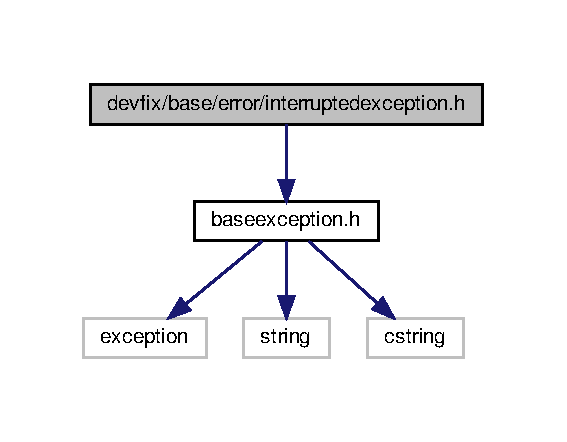
\includegraphics[width=272pt]{interruptedexception_8h__incl}
\end{center}
\end{figure}
This graph shows which files directly or indirectly include this file\+:\nopagebreak
\begin{figure}[H]
\begin{center}
\leavevmode
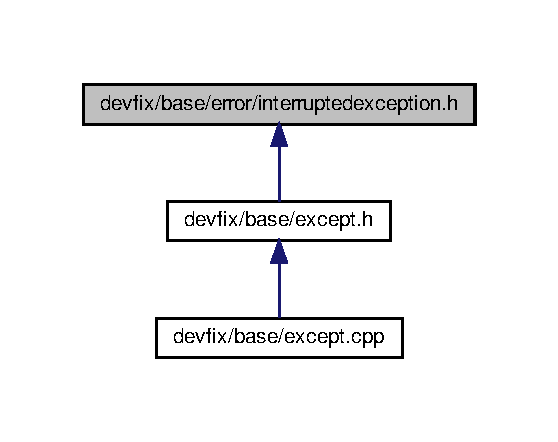
\includegraphics[width=268pt]{interruptedexception_8h__dep__incl}
\end{center}
\end{figure}
\subsection*{Classes}
\begin{DoxyCompactItemize}
\item 
struct \hyperlink{structdevfix_1_1base_1_1error_1_1interruptedexception}{devfix\+::base\+::error\+::interruptedexception}
\begin{DoxyCompactList}\small\item\em Thrown when an operation is interrupted, either before or during the activity. \end{DoxyCompactList}\end{DoxyCompactItemize}
\subsection*{Namespaces}
\begin{DoxyCompactItemize}
\item 
 \hyperlink{namespacedevfix_1_1base_1_1error}{devfix\+::base\+::error}
\begin{DoxyCompactList}\small\item\em Namespace for general errors like timeouts or io failures. \end{DoxyCompactList}\end{DoxyCompactItemize}

\hypertarget{ioexception_8h}{}\section{devfix/base/error/ioexception.h File Reference}
\label{ioexception_8h}\index{devfix/base/error/ioexception.\+h@{devfix/base/error/ioexception.\+h}}
{\ttfamily \#include \char`\"{}baseexception.\+h\char`\"{}}\newline
Include dependency graph for ioexception.\+h\+:\nopagebreak
\begin{figure}[H]
\begin{center}
\leavevmode
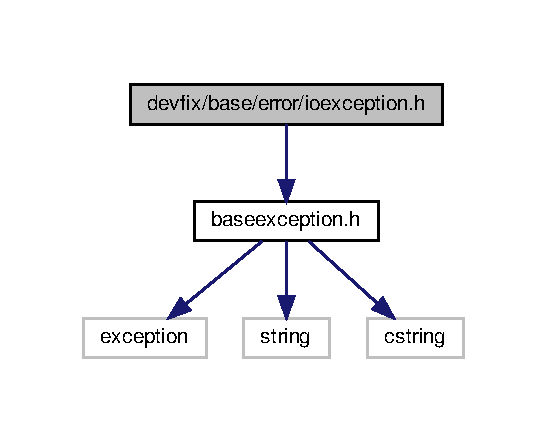
\includegraphics[width=263pt]{ioexception_8h__incl}
\end{center}
\end{figure}
\subsection*{Classes}
\begin{DoxyCompactItemize}
\item 
struct \hyperlink{structdevfix_1_1base_1_1error_1_1ioexception}{devfix\+::base\+::error\+::ioexception}
\begin{DoxyCompactList}\small\item\em Signals that an I/O error of some sort has occurred. \end{DoxyCompactList}\end{DoxyCompactItemize}
\subsection*{Namespaces}
\begin{DoxyCompactItemize}
\item 
 \hyperlink{namespacedevfix_1_1base_1_1error}{devfix\+::base\+::error}
\begin{DoxyCompactList}\small\item\em Namespace for general errors like timeouts or io failures. \end{DoxyCompactList}\end{DoxyCompactItemize}

\hypertarget{base_2error_2namespace_8h}{}\section{devfix/base/error/namespace.h File Reference}
\label{base_2error_2namespace_8h}\index{devfix/base/error/namespace.\+h@{devfix/base/error/namespace.\+h}}
\subsection*{Namespaces}
\begin{DoxyCompactItemize}
\item 
 \hyperlink{namespacedevfix_1_1base_1_1error}{devfix\+::base\+::error}
\begin{DoxyCompactList}\small\item\em Namespace for general errors like timeouts or io failures. \end{DoxyCompactList}\end{DoxyCompactItemize}

\hypertarget{base_2io_2namespace_8h}{}\section{devfix/base/io/namespace.h File Reference}
\label{base_2io_2namespace_8h}\index{devfix/base/io/namespace.\+h@{devfix/base/io/namespace.\+h}}
\subsection*{Namespaces}
\begin{DoxyCompactItemize}
\item 
 \hyperlink{namespacedevfix_1_1base_1_1io}{devfix\+::base\+::io}
\begin{DoxyCompactList}\small\item\em Namespace for io tool, for instance streams. \end{DoxyCompactList}\end{DoxyCompactItemize}

\hypertarget{base_2namespace_8h}{}\section{devfix/base/namespace.h File Reference}
\label{base_2namespace_8h}\index{devfix/base/namespace.\+h@{devfix/base/namespace.\+h}}
\subsection*{Namespaces}
\begin{DoxyCompactItemize}
\item 
 \hyperlink{namespacedevfix}{devfix}
\item 
 \hyperlink{namespacedevfix_1_1base}{devfix\+::base}
\begin{DoxyCompactList}\small\item\em Root namespace of devfix base library. \end{DoxyCompactList}\end{DoxyCompactItemize}

\hypertarget{net_2namespace_8h}{}\section{devfix/net/namespace.h File Reference}
\label{net_2namespace_8h}\index{devfix/net/namespace.\+h@{devfix/net/namespace.\+h}}
\subsection*{Namespaces}
\begin{DoxyCompactItemize}
\item 
 \hyperlink{namespacedevfix}{devfix}
\item 
 \hyperlink{namespacedevfix_1_1net}{devfix\+::net}
\begin{DoxyCompactList}\small\item\em Root namespace of devfix network library. \end{DoxyCompactList}\end{DoxyCompactItemize}

\hypertarget{timeoutexception_8h}{}\section{devfix/base/error/timeoutexception.h File Reference}
\label{timeoutexception_8h}\index{devfix/base/error/timeoutexception.\+h@{devfix/base/error/timeoutexception.\+h}}
{\ttfamily \#include \char`\"{}baseexception.\+h\char`\"{}}\newline
Include dependency graph for timeoutexception.\+h\+:\nopagebreak
\begin{figure}[H]
\begin{center}
\leavevmode
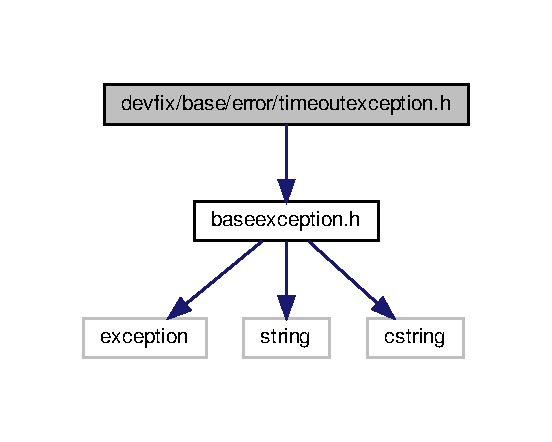
\includegraphics[width=265pt]{timeoutexception_8h__incl}
\end{center}
\end{figure}
This graph shows which files directly or indirectly include this file\+:\nopagebreak
\begin{figure}[H]
\begin{center}
\leavevmode
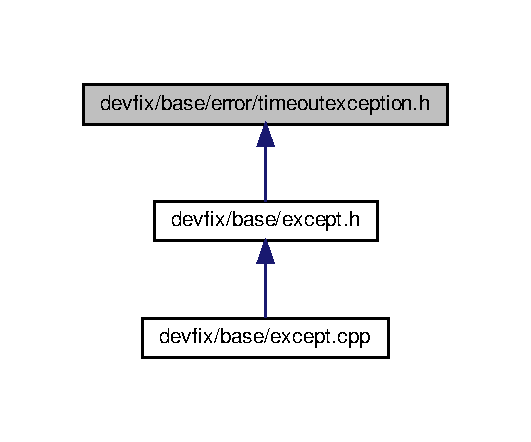
\includegraphics[width=255pt]{timeoutexception_8h__dep__incl}
\end{center}
\end{figure}
\subsection*{Classes}
\begin{DoxyCompactItemize}
\item 
struct \hyperlink{structdevfix_1_1base_1_1error_1_1timeoutexception}{devfix\+::base\+::error\+::timeoutexception}
\begin{DoxyCompactList}\small\item\em Exception thrown when a blocking operation times out. \end{DoxyCompactList}\end{DoxyCompactItemize}
\subsection*{Namespaces}
\begin{DoxyCompactItemize}
\item 
 \hyperlink{namespacedevfix_1_1base_1_1error}{devfix\+::base\+::error}
\begin{DoxyCompactList}\small\item\em Namespace for general errors like timeouts or io failures. \end{DoxyCompactList}\end{DoxyCompactItemize}

\hypertarget{filesystem_8h}{}\section{devfix/base/filesystem.h File Reference}
\label{filesystem_8h}\index{devfix/base/filesystem.\+h@{devfix/base/filesystem.\+h}}
{\ttfamily \#include $<$string$>$}\newline
{\ttfamily \#include $<$list$>$}\newline
Include dependency graph for filesystem.\+h\+:\nopagebreak
\begin{figure}[H]
\begin{center}
\leavevmode
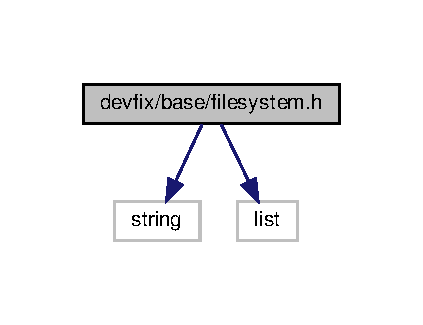
\includegraphics[width=203pt]{filesystem_8h__incl}
\end{center}
\end{figure}
\subsection*{Classes}
\begin{DoxyCompactItemize}
\item 
struct \hyperlink{structdevfix_1_1base_1_1filesystem}{devfix\+::base\+::filesystem}
\end{DoxyCompactItemize}
\subsection*{Namespaces}
\begin{DoxyCompactItemize}
\item 
 \hyperlink{namespacedevfix_1_1base}{devfix\+::base}
\begin{DoxyCompactList}\small\item\em Root namespace of devfix base library. \end{DoxyCompactList}\end{DoxyCompactItemize}

\hypertarget{foldt_8h}{}\section{devfix/base/foldt.h File Reference}
\label{foldt_8h}\index{devfix/base/foldt.\+h@{devfix/base/foldt.\+h}}
This graph shows which files directly or indirectly include this file\+:
\nopagebreak
\begin{figure}[H]
\begin{center}
\leavevmode
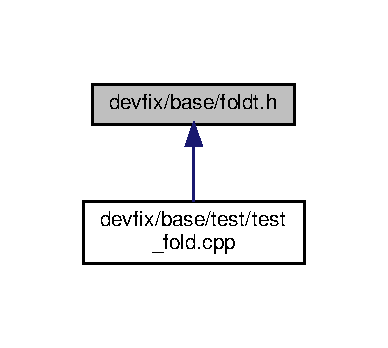
\includegraphics[width=186pt]{foldt_8h__dep__incl}
\end{center}
\end{figure}
\subsection*{Functions}
\begin{DoxyCompactItemize}
\item 
{\footnotesize template$<$typename Y , typename F , typename , typename ... Xs$>$ }\\Y \hyperlink{foldt_8h_a0663368800f70a8be80c4218d480fab7}{foldt} (Y n, F f, Xs... xs)
\begin{DoxyCompactList}\small\item\em Uses a given combining operation, recombines the results of recursively processing its constituent parts, building up a return value. \end{DoxyCompactList}\item 
{\footnotesize template$<$typename Y , typename F $>$ }\\Y \hyperlink{foldt_8h_aec2302afd6b7c1f2b8b829b0d69888b6}{foldt} (Y n, F)
\item 
{\footnotesize template$<$typename Y , typename F , typename X , typename ... Xs$>$ }\\Y \hyperlink{foldt_8h_a2ed7c654c955614467c1390d46942ea0}{foldt} (Y n, F f, X x, Xs... xs)
\end{DoxyCompactItemize}


\subsection{Function Documentation}
\mbox{\Hypertarget{foldt_8h_a0663368800f70a8be80c4218d480fab7}\label{foldt_8h_a0663368800f70a8be80c4218d480fab7}} 
\index{foldt.\+h@{foldt.\+h}!foldt@{foldt}}
\index{foldt@{foldt}!foldt.\+h@{foldt.\+h}}
\subsubsection{\texorpdfstring{foldt()}{foldt()}\hspace{0.1cm}{\footnotesize\ttfamily [1/3]}}
{\footnotesize\ttfamily template$<$typename Y , typename F , typename , typename ... Xs$>$ \\
Y foldt (\begin{DoxyParamCaption}\item[{Y}]{n,  }\item[{F}]{f,  }\item[{Xs...}]{xs }\end{DoxyParamCaption})}



Uses a given combining operation, recombines the results of recursively processing its constituent parts, building up a return value. 


\begin{DoxyTemplParams}{Template Parameters}
{\em Y} & return type \\
\hline
{\em F} & type of combining function \\
\hline
{\em Xs} & type argument parameter pack \\
\hline
\end{DoxyTemplParams}

\begin{DoxyParams}{Parameters}
{\em n} & neutral element \\
\hline
{\em f} & combining function \\
\hline
{\em xs} & argument parameter pack \\
\hline
\end{DoxyParams}
\begin{DoxyReturn}{Returns}
result 
\end{DoxyReturn}
Here is the caller graph for this function\+:
\nopagebreak
\begin{figure}[H]
\begin{center}
\leavevmode
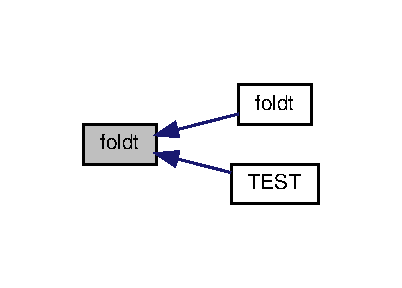
\includegraphics[width=193pt]{foldt_8h_a0663368800f70a8be80c4218d480fab7_icgraph}
\end{center}
\end{figure}
\mbox{\Hypertarget{foldt_8h_aec2302afd6b7c1f2b8b829b0d69888b6}\label{foldt_8h_aec2302afd6b7c1f2b8b829b0d69888b6}} 
\index{foldt.\+h@{foldt.\+h}!foldt@{foldt}}
\index{foldt@{foldt}!foldt.\+h@{foldt.\+h}}
\subsubsection{\texorpdfstring{foldt()}{foldt()}\hspace{0.1cm}{\footnotesize\ttfamily [2/3]}}
{\footnotesize\ttfamily template$<$typename Y , typename F $>$ \\
Y foldt (\begin{DoxyParamCaption}\item[{Y}]{n,  }\item[{F}]{ }\end{DoxyParamCaption})}

\mbox{\Hypertarget{foldt_8h_a2ed7c654c955614467c1390d46942ea0}\label{foldt_8h_a2ed7c654c955614467c1390d46942ea0}} 
\index{foldt.\+h@{foldt.\+h}!foldt@{foldt}}
\index{foldt@{foldt}!foldt.\+h@{foldt.\+h}}
\subsubsection{\texorpdfstring{foldt()}{foldt()}\hspace{0.1cm}{\footnotesize\ttfamily [3/3]}}
{\footnotesize\ttfamily template$<$typename Y , typename F , typename X , typename ... Xs$>$ \\
Y foldt (\begin{DoxyParamCaption}\item[{Y}]{n,  }\item[{F}]{f,  }\item[{X}]{x,  }\item[{Xs...}]{xs }\end{DoxyParamCaption})}


\hypertarget{interpolation_8h}{}\section{devfix/base/interpolation.h File Reference}
\label{interpolation_8h}\index{devfix/base/interpolation.\+h@{devfix/base/interpolation.\+h}}
{\ttfamily \#include $<$vector$>$}\newline
{\ttfamily \#include $<$stdexcept$>$}\newline
Include dependency graph for interpolation.\+h\+:\nopagebreak
\begin{figure}[H]
\begin{center}
\leavevmode
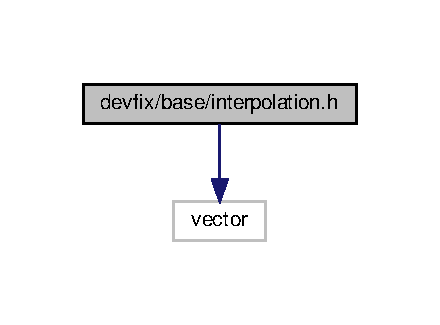
\includegraphics[width=211pt]{interpolation_8h__incl}
\end{center}
\end{figure}
\subsection*{Classes}
\begin{DoxyCompactItemize}
\item 
struct \hyperlink{structdevfix_1_1base_1_1interpolation}{devfix\+::base\+::interpolation$<$ Float\+T $>$}
\end{DoxyCompactItemize}
\subsection*{Namespaces}
\begin{DoxyCompactItemize}
\item 
 \hyperlink{namespacedevfix_1_1base}{devfix\+::base}
\begin{DoxyCompactList}\small\item\em Root namespace of devfix base library. \end{DoxyCompactList}\end{DoxyCompactItemize}

\hypertarget{inputstream_8h}{}\section{devfix/base/io/inputstream.h File Reference}
\label{inputstream_8h}\index{devfix/base/io/inputstream.\+h@{devfix/base/io/inputstream.\+h}}
{\ttfamily \#include $<$cstdint$>$}\newline
Include dependency graph for inputstream.\+h\+:\nopagebreak
\begin{figure}[H]
\begin{center}
\leavevmode
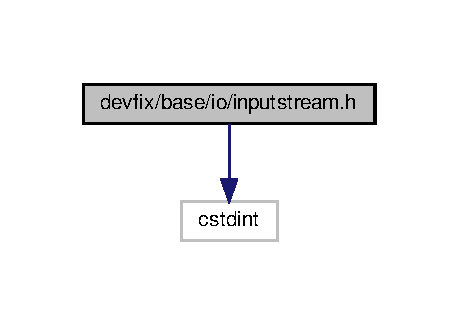
\includegraphics[width=220pt]{inputstream_8h__incl}
\end{center}
\end{figure}
This graph shows which files directly or indirectly include this file\+:\nopagebreak
\begin{figure}[H]
\begin{center}
\leavevmode
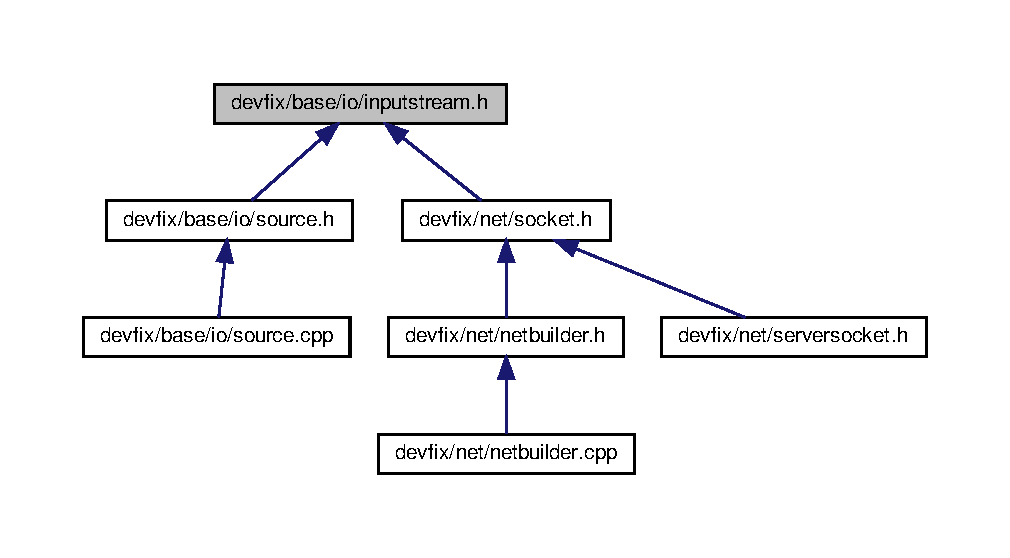
\includegraphics[width=350pt]{inputstream_8h__dep__incl}
\end{center}
\end{figure}
\subsection*{Classes}
\begin{DoxyCompactItemize}
\item 
struct \hyperlink{structdevfix_1_1base_1_1io_1_1inputstream}{devfix\+::base\+::io\+::inputstream}
\begin{DoxyCompactList}\small\item\em Superclass of all classes representing an input stream of bytes. \end{DoxyCompactList}\end{DoxyCompactItemize}
\subsection*{Namespaces}
\begin{DoxyCompactItemize}
\item 
 \hyperlink{namespacedevfix_1_1base_1_1io}{devfix\+::base\+::io}
\begin{DoxyCompactList}\small\item\em Namespace for io tool, for instance streams. \end{DoxyCompactList}\end{DoxyCompactItemize}

\hypertarget{iotypes_8h}{}\section{devfix/base/io/iotypes.h File Reference}
\label{iotypes_8h}\index{devfix/base/io/iotypes.\+h@{devfix/base/io/iotypes.\+h}}
{\ttfamily \#include $<$functional$>$}\newline
Include dependency graph for iotypes.\+h\+:\nopagebreak
\begin{figure}[H]
\begin{center}
\leavevmode
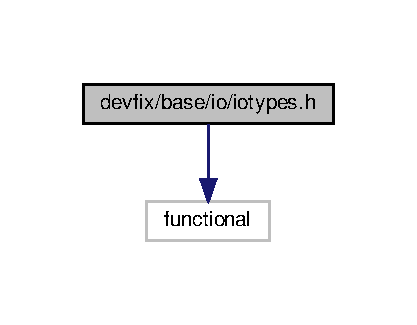
\includegraphics[width=200pt]{iotypes_8h__incl}
\end{center}
\end{figure}
This graph shows which files directly or indirectly include this file\+:\nopagebreak
\begin{figure}[H]
\begin{center}
\leavevmode
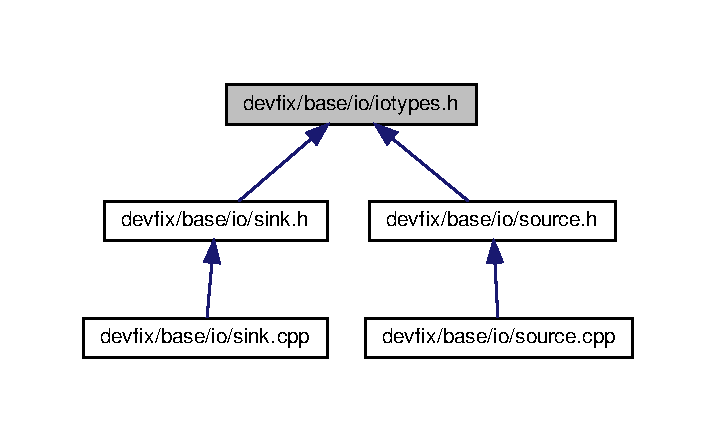
\includegraphics[width=344pt]{iotypes_8h__dep__incl}
\end{center}
\end{figure}
\subsection*{Namespaces}
\begin{DoxyCompactItemize}
\item 
 \hyperlink{namespacedevfix_1_1base_1_1io}{devfix\+::base\+::io}
\begin{DoxyCompactList}\small\item\em Namespace for io tool, for instance streams. \end{DoxyCompactList}\end{DoxyCompactItemize}
\subsection*{Typedefs}
\begin{DoxyCompactItemize}
\item 
typedef std\+::function$<$ void()$>$ \hyperlink{namespacedevfix_1_1base_1_1io_ae3118387742e5f4d484a328a213d6a5d}{devfix\+::base\+::io\+::close\+\_\+t}
\item 
typedef std\+::function$<$ bool()$>$ \hyperlink{namespacedevfix_1_1base_1_1io_a14f89d4437ced6ede49c044ee8e71f17}{devfix\+::base\+::io\+::is\+\_\+closed\+\_\+t}
\item 
typedef std\+::function$<$ void(void $\ast$, std\+::size\+\_\+t)$>$ \hyperlink{namespacedevfix_1_1base_1_1io_afa65222ee5a1636be18df5e16bbcf858}{devfix\+::base\+::io\+::read\+\_\+t}
\item 
typedef std\+::function$<$ void(std\+::size\+\_\+t)$>$ \hyperlink{namespacedevfix_1_1base_1_1io_aeb8f94d85cfeaa405f53a6967e609645}{devfix\+::base\+::io\+::skip\+\_\+t}
\item 
typedef std\+::function$<$ std\+::size\+\_\+t()$>$ \hyperlink{namespacedevfix_1_1base_1_1io_a19c1195ab6a44e6d4f48b86062860a11}{devfix\+::base\+::io\+::available\+\_\+t}
\item 
typedef std\+::function$<$ void(const void $\ast$, std\+::size\+\_\+t)$>$ \hyperlink{namespacedevfix_1_1base_1_1io_a75953e4d7f81d76e419f9672ffedda87}{devfix\+::base\+::io\+::write\+\_\+t}
\item 
typedef std\+::function$<$ void()$>$ \hyperlink{namespacedevfix_1_1base_1_1io_a622685976c7f503411827fba028d3ce1}{devfix\+::base\+::io\+::flush\+\_\+t}
\end{DoxyCompactItemize}
\subsection*{Variables}
\begin{DoxyCompactItemize}
\item 
const close\+\_\+t \hyperlink{namespacedevfix_1_1base_1_1io_a14a286c17d4b93881d42b1d14beb2d0b}{devfix\+::base\+::io\+::\+D\+E\+F\+A\+U\+L\+T\+\_\+\+C\+L\+O\+SE} = \mbox{[}$\,$\mbox{]}() \{\}
\item 
const is\+\_\+closed\+\_\+t \hyperlink{namespacedevfix_1_1base_1_1io_ae04fec2a2a2db3482e624a59e59a2a14}{devfix\+::base\+::io\+::\+D\+E\+F\+A\+U\+L\+T\+\_\+\+I\+S\+\_\+\+C\+L\+O\+S\+ED} = \mbox{[}$\,$\mbox{]}() \{ return false; \}
\end{DoxyCompactItemize}

\hypertarget{outputstream_8h}{}\section{devfix/base/io/outputstream.h File Reference}
\label{outputstream_8h}\index{devfix/base/io/outputstream.\+h@{devfix/base/io/outputstream.\+h}}
{\ttfamily \#include $<$cstddef$>$}\newline
Include dependency graph for outputstream.\+h\+:\nopagebreak
\begin{figure}[H]
\begin{center}
\leavevmode
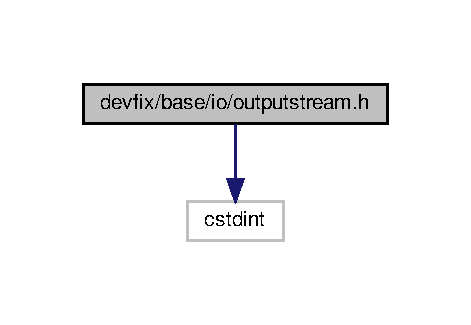
\includegraphics[width=226pt]{outputstream_8h__incl}
\end{center}
\end{figure}
This graph shows which files directly or indirectly include this file\+:\nopagebreak
\begin{figure}[H]
\begin{center}
\leavevmode
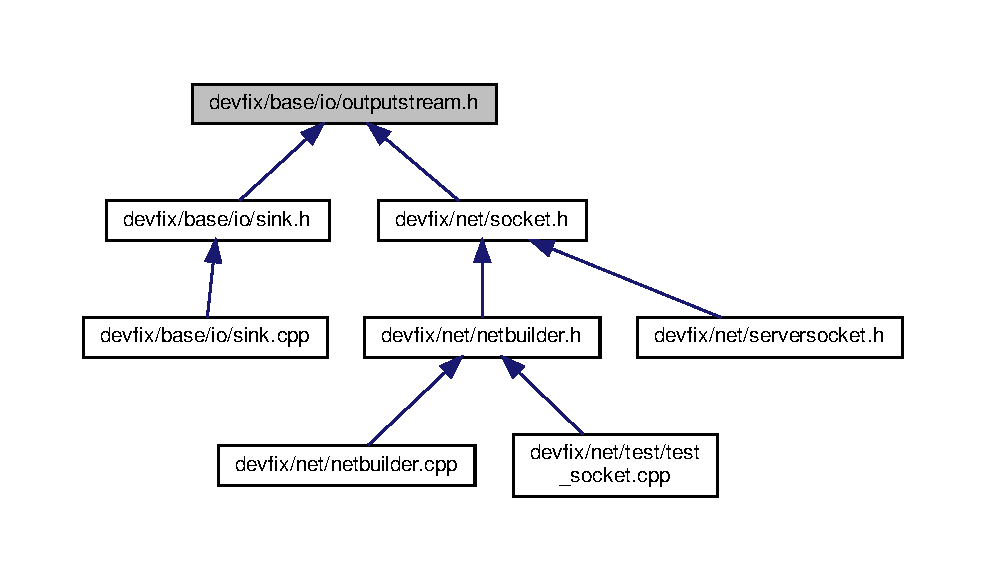
\includegraphics[width=350pt]{outputstream_8h__dep__incl}
\end{center}
\end{figure}
\subsection*{Classes}
\begin{DoxyCompactItemize}
\item 
struct \hyperlink{structdevfix_1_1base_1_1io_1_1outputstream}{devfix\+::base\+::io\+::outputstream}
\begin{DoxyCompactList}\small\item\em Superclass of all classes representing an output stream of bytes. \end{DoxyCompactList}\end{DoxyCompactItemize}
\subsection*{Namespaces}
\begin{DoxyCompactItemize}
\item 
 \hyperlink{namespacedevfix_1_1base_1_1io}{devfix\+::base\+::io}
\begin{DoxyCompactList}\small\item\em Namespace for io tool, for instance streams. \end{DoxyCompactList}\end{DoxyCompactItemize}

\hypertarget{sink_8cpp}{}\section{devfix/base/io/sink.cpp File Reference}
\label{sink_8cpp}\index{devfix/base/io/sink.\+cpp@{devfix/base/io/sink.\+cpp}}
{\ttfamily \#include \char`\"{}sink.\+h\char`\"{}}\newline
{\ttfamily \#include $<$utility$>$}\newline
Include dependency graph for sink.\+cpp\+:\nopagebreak
\begin{figure}[H]
\begin{center}
\leavevmode
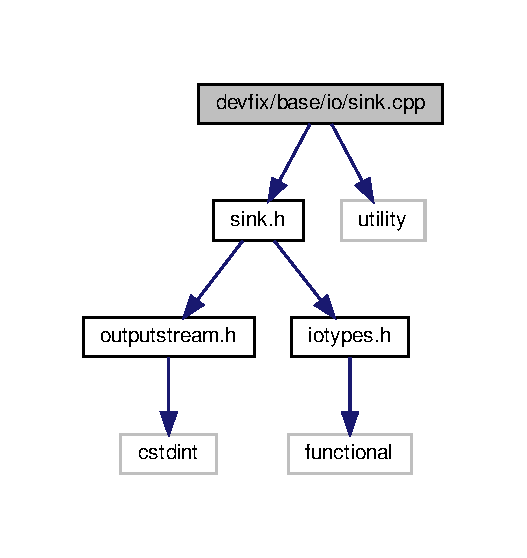
\includegraphics[width=253pt]{sink_8cpp__incl}
\end{center}
\end{figure}
\subsection*{Namespaces}
\begin{DoxyCompactItemize}
\item 
 \hyperlink{namespacedevfix_1_1base_1_1io}{devfix\+::base\+::io}
\begin{DoxyCompactList}\small\item\em Namespace for io tool, for instance streams. \end{DoxyCompactList}\end{DoxyCompactItemize}

\hypertarget{sink_8h}{}\section{devfix/base/io/sink.h File Reference}
\label{sink_8h}\index{devfix/base/io/sink.\+h@{devfix/base/io/sink.\+h}}
{\ttfamily \#include \char`\"{}outputstream.\+h\char`\"{}}\newline
{\ttfamily \#include \char`\"{}iotypes.\+h\char`\"{}}\newline
Include dependency graph for sink.\+h\+:\nopagebreak
\begin{figure}[H]
\begin{center}
\leavevmode
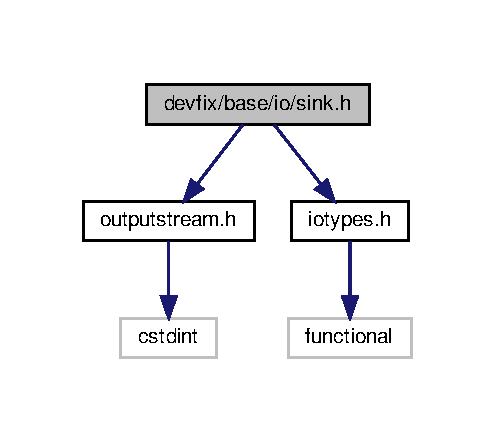
\includegraphics[width=238pt]{sink_8h__incl}
\end{center}
\end{figure}
This graph shows which files directly or indirectly include this file\+:\nopagebreak
\begin{figure}[H]
\begin{center}
\leavevmode
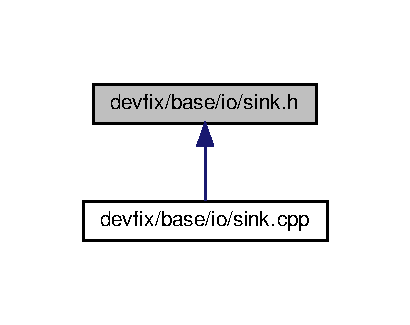
\includegraphics[width=197pt]{sink_8h__dep__incl}
\end{center}
\end{figure}
\subsection*{Classes}
\begin{DoxyCompactItemize}
\item 
struct \hyperlink{structdevfix_1_1base_1_1io_1_1sink}{devfix\+::base\+::io\+::sink}
\begin{DoxyCompactList}\small\item\em Adapter class to create an {\itshape outputstream} from function pointers. \end{DoxyCompactList}\end{DoxyCompactItemize}
\subsection*{Namespaces}
\begin{DoxyCompactItemize}
\item 
 \hyperlink{namespacedevfix_1_1base_1_1io}{devfix\+::base\+::io}
\begin{DoxyCompactList}\small\item\em Namespace for io tool, for instance streams. \end{DoxyCompactList}\end{DoxyCompactItemize}

\hypertarget{source_8cpp}{}\section{devfix/base/io/source.cpp File Reference}
\label{source_8cpp}\index{devfix/base/io/source.\+cpp@{devfix/base/io/source.\+cpp}}
{\ttfamily \#include \char`\"{}source.\+h\char`\"{}}\newline
Include dependency graph for source.\+cpp\+:\nopagebreak
\begin{figure}[H]
\begin{center}
\leavevmode
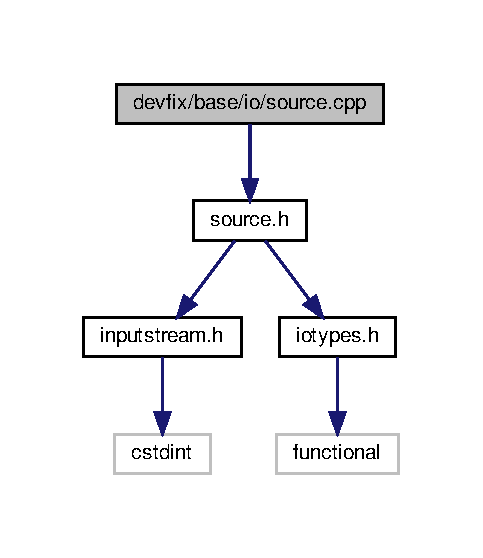
\includegraphics[width=232pt]{source_8cpp__incl}
\end{center}
\end{figure}
\subsection*{Namespaces}
\begin{DoxyCompactItemize}
\item 
 \hyperlink{namespacedevfix_1_1base_1_1io}{devfix\+::base\+::io}
\begin{DoxyCompactList}\small\item\em Namespace for io tool, for instance streams. \end{DoxyCompactList}\end{DoxyCompactItemize}

\hypertarget{source_8h}{}\section{devfix/base/io/source.h File Reference}
\label{source_8h}\index{devfix/base/io/source.\+h@{devfix/base/io/source.\+h}}
{\ttfamily \#include \char`\"{}inputstream.\+h\char`\"{}}\newline
{\ttfamily \#include \char`\"{}iotypes.\+h\char`\"{}}\newline
Include dependency graph for source.\+h\+:\nopagebreak
\begin{figure}[H]
\begin{center}
\leavevmode
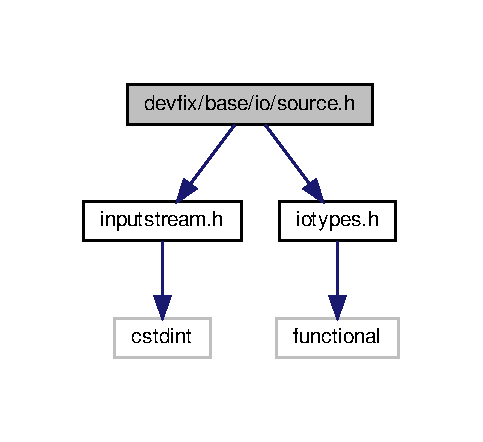
\includegraphics[width=232pt]{source_8h__incl}
\end{center}
\end{figure}
This graph shows which files directly or indirectly include this file\+:\nopagebreak
\begin{figure}[H]
\begin{center}
\leavevmode
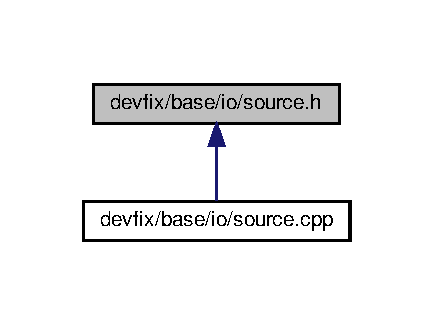
\includegraphics[width=208pt]{source_8h__dep__incl}
\end{center}
\end{figure}
\subsection*{Classes}
\begin{DoxyCompactItemize}
\item 
struct \hyperlink{structdevfix_1_1base_1_1io_1_1source}{devfix\+::base\+::io\+::source}
\begin{DoxyCompactList}\small\item\em Adapter class to create an {\itshape inputstream} from function pointers. \end{DoxyCompactList}\end{DoxyCompactItemize}
\subsection*{Namespaces}
\begin{DoxyCompactItemize}
\item 
 \hyperlink{namespacedevfix_1_1base_1_1io}{devfix\+::base\+::io}
\begin{DoxyCompactList}\small\item\em Namespace for io tool, for instance streams. \end{DoxyCompactList}\end{DoxyCompactItemize}

\hypertarget{lnx_2filesystem_8cpp}{}\section{devfix/base/lnx/filesystem.cpp File Reference}
\label{lnx_2filesystem_8cpp}\index{devfix/base/lnx/filesystem.\+cpp@{devfix/base/lnx/filesystem.\+cpp}}
{\ttfamily \#include \char`\"{}../platform.\+h\char`\"{}}\newline
Include dependency graph for filesystem.\+cpp\+:\nopagebreak
\begin{figure}[H]
\begin{center}
\leavevmode
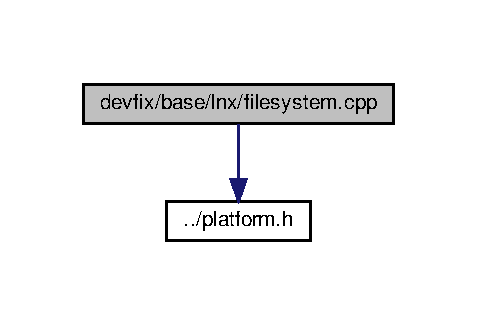
\includegraphics[width=229pt]{lnx_2filesystem_8cpp__incl}
\end{center}
\end{figure}

\hypertarget{win_2filesystem_8cpp}{}\section{devfix/base/win/filesystem.cpp File Reference}
\label{win_2filesystem_8cpp}\index{devfix/base/win/filesystem.\+cpp@{devfix/base/win/filesystem.\+cpp}}
{\ttfamily \#include \char`\"{}../platform.\+h\char`\"{}}\newline
Include dependency graph for filesystem.\+cpp\+:
\nopagebreak
\begin{figure}[H]
\begin{center}
\leavevmode
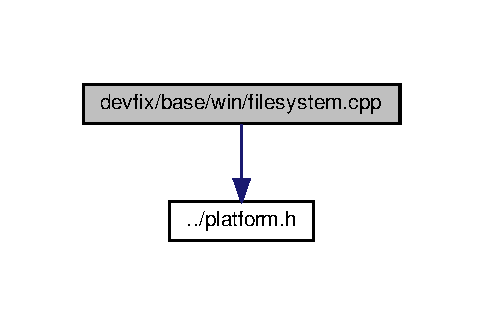
\includegraphics[width=232pt]{win_2filesystem_8cpp__incl}
\end{center}
\end{figure}

\hypertarget{math_8h}{}\section{devfix/base/math.h File Reference}
\label{math_8h}\index{devfix/base/math.\+h@{devfix/base/math.\+h}}
{\ttfamily \#include $<$cstdint$>$}\newline
Include dependency graph for math.\+h\+:\nopagebreak
\begin{figure}[H]
\begin{center}
\leavevmode
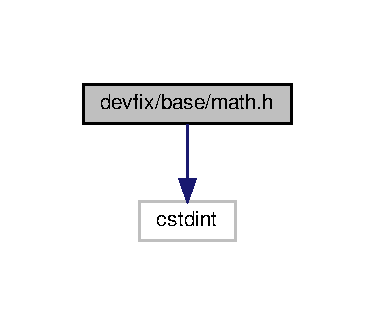
\includegraphics[width=180pt]{math_8h__incl}
\end{center}
\end{figure}
This graph shows which files directly or indirectly include this file\+:\nopagebreak
\begin{figure}[H]
\begin{center}
\leavevmode
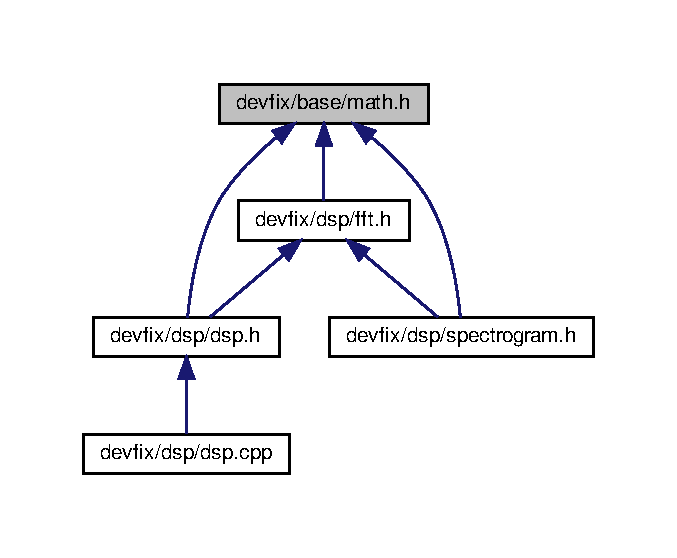
\includegraphics[width=207pt]{math_8h__dep__incl}
\end{center}
\end{figure}
\subsection*{Classes}
\begin{DoxyCompactItemize}
\item 
struct \hyperlink{structdevfix_1_1base_1_1__math_1_1Table}{devfix\+::base\+::\+\_\+math\+::\+Table$<$ T, N, G, Args $>$}
\item 
struct \hyperlink{structdevfix_1_1base_1_1math}{devfix\+::base\+::math}
\end{DoxyCompactItemize}
\subsection*{Namespaces}
\begin{DoxyCompactItemize}
\item 
 \hyperlink{namespacedevfix_1_1base}{devfix\+::base}
\begin{DoxyCompactList}\small\item\em Root namespace of devfix base library. \end{DoxyCompactList}\item 
 \hyperlink{namespacedevfix_1_1base_1_1__math}{devfix\+::base\+::\+\_\+math}
\end{DoxyCompactItemize}

\hypertarget{memory_8h}{}\section{devfix/base/memory.h File Reference}
\label{memory_8h}\index{devfix/base/memory.\+h@{devfix/base/memory.\+h}}
{\ttfamily \#include $<$memory$>$}\newline
Include dependency graph for memory.\+h\+:\nopagebreak
\begin{figure}[H]
\begin{center}
\leavevmode
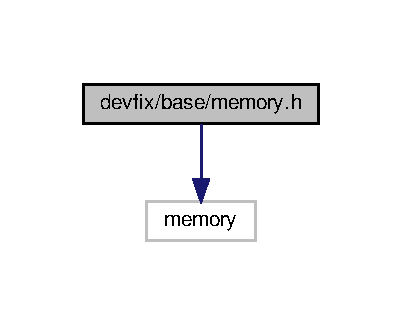
\includegraphics[width=193pt]{memory_8h__incl}
\end{center}
\end{figure}
This graph shows which files directly or indirectly include this file\+:\nopagebreak
\begin{figure}[H]
\begin{center}
\leavevmode
\includegraphics[width=343pt]{memory_8h__dep__incl}
\end{center}
\end{figure}
\subsection*{Namespaces}
\begin{DoxyCompactItemize}
\item 
 \hyperlink{namespacedevfix_1_1base}{devfix\+::base}
\begin{DoxyCompactList}\small\item\em Root namespace of devfix base library. \end{DoxyCompactList}\end{DoxyCompactItemize}
\subsection*{Typedefs}
\begin{DoxyCompactItemize}
\item 
{\footnotesize template$<$class T $>$ }\\using \hyperlink{namespacedevfix_1_1base_a18dfbd492717795cee1cfa6f14a8f724}{devfix\+::base\+::up} = std\+::unique\+\_\+ptr$<$ T $>$
\begin{DoxyCompactList}\small\item\em Alias for std\+::unique\+\_\+ptr. \end{DoxyCompactList}\item 
{\footnotesize template$<$class T $>$ }\\using \hyperlink{namespacedevfix_1_1base_ad239a07977b9e77ffabaf558636d0b8b}{devfix\+::base\+::sp} = std\+::shared\+\_\+ptr$<$ T $>$
\begin{DoxyCompactList}\small\item\em Alias for std\+::shared\+\_\+ptr. \end{DoxyCompactList}\end{DoxyCompactItemize}

\hypertarget{platform_8h}{}\section{devfix/base/platform.h File Reference}
\label{platform_8h}\index{devfix/base/platform.\+h@{devfix/base/platform.\+h}}
This graph shows which files directly or indirectly include this file\+:\nopagebreak
\begin{figure}[H]
\begin{center}
\leavevmode
\includegraphics[width=350pt]{platform_8h__dep__incl}
\end{center}
\end{figure}
\subsection*{Macros}
\begin{DoxyCompactItemize}
\item 
\#define \hyperlink{platform_8h_affcc3790504b838f9ce56a008cce0950}{P\+L\+A\+T\+F\+O\+R\+M\+\_\+\+L\+I\+N\+UX}~0
\item 
\#define \hyperlink{platform_8h_a20cd3c4775f1897fb5658d2dc61382c3}{P\+L\+A\+T\+F\+O\+R\+M\+\_\+\+W\+I\+N\+D\+O\+WS}~0
\item 
\#define \hyperlink{platform_8h_a0bba118331fd3ff9e1ad80b92a75b345}{E\+R\+R\+O\+R\+\_\+\+P\+L\+A\+T\+F\+O\+R\+M\+\_\+\+U\+N\+S\+U\+P\+P\+O\+R\+T\+ED}~static\+\_\+assert ( false, \char`\"{}Platform not supported\char`\"{} )
\item 
\#define \hyperlink{platform_8h_a5fccb4fc71e44089a1b1a77fc76c0b68}{\+\_\+\+\_\+\+F\+I\+L\+E\+N\+A\+M\+E\+\_\+\+\_\+}~\&\+\_\+\+\_\+\+F\+I\+L\+E\+\_\+\+\_\+\mbox{[}0\mbox{]}
\item 
\#define \hyperlink{platform_8h_acf16e3e245e0e3b5d45b2a11075d4d36}{S\+O\+U\+R\+C\+E\+\_\+\+L\+I\+NE}~std\+::string(\hyperlink{platform_8h_a5fccb4fc71e44089a1b1a77fc76c0b68}{\+\_\+\+\_\+\+F\+I\+L\+E\+N\+A\+M\+E\+\_\+\+\_\+}) + \char`\"{}\+:\char`\"{} + std\+::to\+\_\+string(\+\_\+\+\_\+\+L\+I\+N\+E\+\_\+\+\_\+) + \char`\"{}\+: in \textbackslash{}\char`\"{}\char`\"{} + std\+::string(\&\+\_\+\+\_\+\+F\+U\+N\+C\+T\+I\+O\+N\+\_\+\+\_\+\mbox{[}0\mbox{]}) + \char`\"{}\textbackslash{}\char`\"{}\char`\"{}
\item 
\#define \hyperlink{platform_8h_a05a7b30aaf65db56c27346272aa681e5}{N\+O\+T\+\_\+\+U\+S\+ED}(x)~static\+\_\+cast$<$void$>$(x)
\end{DoxyCompactItemize}


\subsection{Macro Definition Documentation}
\mbox{\Hypertarget{platform_8h_a5fccb4fc71e44089a1b1a77fc76c0b68}\label{platform_8h_a5fccb4fc71e44089a1b1a77fc76c0b68}} 
\index{platform.\+h@{platform.\+h}!\+\_\+\+\_\+\+F\+I\+L\+E\+N\+A\+M\+E\+\_\+\+\_\+@{\+\_\+\+\_\+\+F\+I\+L\+E\+N\+A\+M\+E\+\_\+\+\_\+}}
\index{\+\_\+\+\_\+\+F\+I\+L\+E\+N\+A\+M\+E\+\_\+\+\_\+@{\+\_\+\+\_\+\+F\+I\+L\+E\+N\+A\+M\+E\+\_\+\+\_\+}!platform.\+h@{platform.\+h}}
\subsubsection{\texorpdfstring{\+\_\+\+\_\+\+F\+I\+L\+E\+N\+A\+M\+E\+\_\+\+\_\+}{\_\_FILENAME\_\_}}
{\footnotesize\ttfamily \#define \+\_\+\+\_\+\+F\+I\+L\+E\+N\+A\+M\+E\+\_\+\+\_\+~\&\+\_\+\+\_\+\+F\+I\+L\+E\+\_\+\+\_\+\mbox{[}0\mbox{]}}

\mbox{\Hypertarget{platform_8h_a0bba118331fd3ff9e1ad80b92a75b345}\label{platform_8h_a0bba118331fd3ff9e1ad80b92a75b345}} 
\index{platform.\+h@{platform.\+h}!E\+R\+R\+O\+R\+\_\+\+P\+L\+A\+T\+F\+O\+R\+M\+\_\+\+U\+N\+S\+U\+P\+P\+O\+R\+T\+ED@{E\+R\+R\+O\+R\+\_\+\+P\+L\+A\+T\+F\+O\+R\+M\+\_\+\+U\+N\+S\+U\+P\+P\+O\+R\+T\+ED}}
\index{E\+R\+R\+O\+R\+\_\+\+P\+L\+A\+T\+F\+O\+R\+M\+\_\+\+U\+N\+S\+U\+P\+P\+O\+R\+T\+ED@{E\+R\+R\+O\+R\+\_\+\+P\+L\+A\+T\+F\+O\+R\+M\+\_\+\+U\+N\+S\+U\+P\+P\+O\+R\+T\+ED}!platform.\+h@{platform.\+h}}
\subsubsection{\texorpdfstring{E\+R\+R\+O\+R\+\_\+\+P\+L\+A\+T\+F\+O\+R\+M\+\_\+\+U\+N\+S\+U\+P\+P\+O\+R\+T\+ED}{ERROR\_PLATFORM\_UNSUPPORTED}}
{\footnotesize\ttfamily \#define E\+R\+R\+O\+R\+\_\+\+P\+L\+A\+T\+F\+O\+R\+M\+\_\+\+U\+N\+S\+U\+P\+P\+O\+R\+T\+ED~static\+\_\+assert ( false, \char`\"{}Platform not supported\char`\"{} )}

\mbox{\Hypertarget{platform_8h_a05a7b30aaf65db56c27346272aa681e5}\label{platform_8h_a05a7b30aaf65db56c27346272aa681e5}} 
\index{platform.\+h@{platform.\+h}!N\+O\+T\+\_\+\+U\+S\+ED@{N\+O\+T\+\_\+\+U\+S\+ED}}
\index{N\+O\+T\+\_\+\+U\+S\+ED@{N\+O\+T\+\_\+\+U\+S\+ED}!platform.\+h@{platform.\+h}}
\subsubsection{\texorpdfstring{N\+O\+T\+\_\+\+U\+S\+ED}{NOT\_USED}}
{\footnotesize\ttfamily \#define N\+O\+T\+\_\+\+U\+S\+ED(\begin{DoxyParamCaption}\item[{}]{x }\end{DoxyParamCaption})~static\+\_\+cast$<$void$>$(x)}

\mbox{\Hypertarget{platform_8h_affcc3790504b838f9ce56a008cce0950}\label{platform_8h_affcc3790504b838f9ce56a008cce0950}} 
\index{platform.\+h@{platform.\+h}!P\+L\+A\+T\+F\+O\+R\+M\+\_\+\+L\+I\+N\+UX@{P\+L\+A\+T\+F\+O\+R\+M\+\_\+\+L\+I\+N\+UX}}
\index{P\+L\+A\+T\+F\+O\+R\+M\+\_\+\+L\+I\+N\+UX@{P\+L\+A\+T\+F\+O\+R\+M\+\_\+\+L\+I\+N\+UX}!platform.\+h@{platform.\+h}}
\subsubsection{\texorpdfstring{P\+L\+A\+T\+F\+O\+R\+M\+\_\+\+L\+I\+N\+UX}{PLATFORM\_LINUX}}
{\footnotesize\ttfamily \#define P\+L\+A\+T\+F\+O\+R\+M\+\_\+\+L\+I\+N\+UX~0}

\mbox{\Hypertarget{platform_8h_a20cd3c4775f1897fb5658d2dc61382c3}\label{platform_8h_a20cd3c4775f1897fb5658d2dc61382c3}} 
\index{platform.\+h@{platform.\+h}!P\+L\+A\+T\+F\+O\+R\+M\+\_\+\+W\+I\+N\+D\+O\+WS@{P\+L\+A\+T\+F\+O\+R\+M\+\_\+\+W\+I\+N\+D\+O\+WS}}
\index{P\+L\+A\+T\+F\+O\+R\+M\+\_\+\+W\+I\+N\+D\+O\+WS@{P\+L\+A\+T\+F\+O\+R\+M\+\_\+\+W\+I\+N\+D\+O\+WS}!platform.\+h@{platform.\+h}}
\subsubsection{\texorpdfstring{P\+L\+A\+T\+F\+O\+R\+M\+\_\+\+W\+I\+N\+D\+O\+WS}{PLATFORM\_WINDOWS}}
{\footnotesize\ttfamily \#define P\+L\+A\+T\+F\+O\+R\+M\+\_\+\+W\+I\+N\+D\+O\+WS~0}

\mbox{\Hypertarget{platform_8h_acf16e3e245e0e3b5d45b2a11075d4d36}\label{platform_8h_acf16e3e245e0e3b5d45b2a11075d4d36}} 
\index{platform.\+h@{platform.\+h}!S\+O\+U\+R\+C\+E\+\_\+\+L\+I\+NE@{S\+O\+U\+R\+C\+E\+\_\+\+L\+I\+NE}}
\index{S\+O\+U\+R\+C\+E\+\_\+\+L\+I\+NE@{S\+O\+U\+R\+C\+E\+\_\+\+L\+I\+NE}!platform.\+h@{platform.\+h}}
\subsubsection{\texorpdfstring{S\+O\+U\+R\+C\+E\+\_\+\+L\+I\+NE}{SOURCE\_LINE}}
{\footnotesize\ttfamily \#define S\+O\+U\+R\+C\+E\+\_\+\+L\+I\+NE~std\+::string(\hyperlink{platform_8h_a5fccb4fc71e44089a1b1a77fc76c0b68}{\+\_\+\+\_\+\+F\+I\+L\+E\+N\+A\+M\+E\+\_\+\+\_\+}) + \char`\"{}\+:\char`\"{} + std\+::to\+\_\+string(\+\_\+\+\_\+\+L\+I\+N\+E\+\_\+\+\_\+) + \char`\"{}\+: in \textbackslash{}\char`\"{}\char`\"{} + std\+::string(\&\+\_\+\+\_\+\+F\+U\+N\+C\+T\+I\+O\+N\+\_\+\+\_\+\mbox{[}0\mbox{]}) + \char`\"{}\textbackslash{}\char`\"{}\char`\"{}}


\hypertarget{strout_8h}{}\section{devfix/base/strout.h File Reference}
\label{strout_8h}\index{devfix/base/strout.\+h@{devfix/base/strout.\+h}}
{\ttfamily \#include $<$sstream$>$}\newline
{\ttfamily \#include $<$variant$>$}\newline
{\ttfamily \#include $<$functional$>$}\newline
{\ttfamily \#include \char`\"{}strutil.\+h\char`\"{}}\newline
Include dependency graph for strout.\+h\+:\nopagebreak
\begin{figure}[H]
\begin{center}
\leavevmode
\includegraphics[width=341pt]{strout_8h__incl}
\end{center}
\end{figure}
\subsection*{Classes}
\begin{DoxyCompactItemize}
\item 
struct \hyperlink{structdevfix_1_1base_1_1strout}{devfix\+::base\+::strout$<$ Char\+T, Traits, Allocator $>$}
\end{DoxyCompactItemize}
\subsection*{Namespaces}
\begin{DoxyCompactItemize}
\item 
 \hyperlink{namespacedevfix_1_1base}{devfix\+::base}
\begin{DoxyCompactList}\small\item\em Root namespace of devfix base library. \end{DoxyCompactList}\end{DoxyCompactItemize}

\hypertarget{strutil_8h}{}\section{devfix/base/strutil.h File Reference}
\label{strutil_8h}\index{devfix/base/strutil.\+h@{devfix/base/strutil.\+h}}
{\ttfamily \#include $<$string$>$}\newline
{\ttfamily \#include $<$tuple$>$}\newline
{\ttfamily \#include $<$optional$>$}\newline
{\ttfamily \#include $<$regex$>$}\newline
Include dependency graph for strutil.\+h\+:
\nopagebreak
\begin{figure}[H]
\begin{center}
\leavevmode
\includegraphics[width=305pt]{strutil_8h__incl}
\end{center}
\end{figure}
This graph shows which files directly or indirectly include this file\+:
\nopagebreak
\begin{figure}[H]
\begin{center}
\leavevmode
\includegraphics[width=308pt]{strutil_8h__dep__incl}
\end{center}
\end{figure}
\subsection*{Classes}
\begin{DoxyCompactItemize}
\item 
struct \hyperlink{structdevfix_1_1base_1_1strutil}{devfix\+::base\+::strutil}
\end{DoxyCompactItemize}
\subsection*{Namespaces}
\begin{DoxyCompactItemize}
\item 
 \hyperlink{namespacedevfix_1_1base}{devfix\+::base}
\begin{DoxyCompactList}\small\item\em Root namespace of devfix base library. \end{DoxyCompactList}\end{DoxyCompactItemize}
\subsection*{Macros}
\begin{DoxyCompactItemize}
\item 
\#define \hyperlink{strutil_8h_a72f64e8a28f366adf3cad6c109082271}{M\+U\+L\+T\+I\+S\+T\+R\+I\+NG}(CharT,  str)~\hyperlink{namespacedevfix_1_1base_a84282bc5458412dfed5ce8b039a70519}{devfix\+::base\+::get\+\_\+from\+\_\+multistring}$<$CharT$>$(str, L\#\#str)
\end{DoxyCompactItemize}
\subsection*{Functions}
\begin{DoxyCompactItemize}
\item 
{\footnotesize template$<$typename T $>$ }\\constexpr const T $\ast$ \hyperlink{namespacedevfix_1_1base_a84282bc5458412dfed5ce8b039a70519}{devfix\+::base\+::get\+\_\+from\+\_\+multistring} (const char $\ast$str, const wchar\+\_\+t $\ast$wstr)
\item 
{\footnotesize template$<$$>$ }\\constexpr const char $\ast$ \hyperlink{namespacedevfix_1_1base_a1d6f6a1a767fa54cd6ff94ae14b43e90}{devfix\+::base\+::get\+\_\+from\+\_\+multistring$<$ char $>$} (const char $\ast$str, const wchar\+\_\+t $\ast$wstr)
\item 
{\footnotesize template$<$$>$ }\\constexpr const wchar\+\_\+t $\ast$ \hyperlink{namespacedevfix_1_1base_a100ea64654a747f262206d9e4b31e6f2}{devfix\+::base\+::get\+\_\+from\+\_\+multistring$<$ wchar\+\_\+t $>$} (const char $\ast$str, const wchar\+\_\+t $\ast$wstr)
\end{DoxyCompactItemize}


\subsection{Macro Definition Documentation}
\mbox{\Hypertarget{strutil_8h_a72f64e8a28f366adf3cad6c109082271}\label{strutil_8h_a72f64e8a28f366adf3cad6c109082271}} 
\index{strutil.\+h@{strutil.\+h}!M\+U\+L\+T\+I\+S\+T\+R\+I\+NG@{M\+U\+L\+T\+I\+S\+T\+R\+I\+NG}}
\index{M\+U\+L\+T\+I\+S\+T\+R\+I\+NG@{M\+U\+L\+T\+I\+S\+T\+R\+I\+NG}!strutil.\+h@{strutil.\+h}}
\subsubsection{\texorpdfstring{M\+U\+L\+T\+I\+S\+T\+R\+I\+NG}{MULTISTRING}}
{\footnotesize\ttfamily \#define M\+U\+L\+T\+I\+S\+T\+R\+I\+NG(\begin{DoxyParamCaption}\item[{}]{CharT,  }\item[{}]{str }\end{DoxyParamCaption})~\hyperlink{namespacedevfix_1_1base_a84282bc5458412dfed5ce8b039a70519}{devfix\+::base\+::get\+\_\+from\+\_\+multistring}$<$CharT$>$(str, L\#\#str)}


\hypertarget{test__filesystem_8cpp}{}\section{devfix/base/test/test\+\_\+filesystem.cpp File Reference}
\label{test__filesystem_8cpp}\index{devfix/base/test/test\+\_\+filesystem.\+cpp@{devfix/base/test/test\+\_\+filesystem.\+cpp}}

\hypertarget{test__fold_8cpp}{}\section{devfix/base/test/test\+\_\+fold.cpp File Reference}
\label{test__fold_8cpp}\index{devfix/base/test/test\+\_\+fold.\+cpp@{devfix/base/test/test\+\_\+fold.\+cpp}}

\hypertarget{test__interpolation_8cpp}{}\section{devfix/base/test/test\+\_\+interpolation.cpp File Reference}
\label{test__interpolation_8cpp}\index{devfix/base/test/test\+\_\+interpolation.\+cpp@{devfix/base/test/test\+\_\+interpolation.\+cpp}}

\hypertarget{test__math_8cpp}{}\section{devfix/base/test/test\+\_\+math.cpp File Reference}
\label{test__math_8cpp}\index{devfix/base/test/test\+\_\+math.\+cpp@{devfix/base/test/test\+\_\+math.\+cpp}}

\hypertarget{test__strout_8cpp}{}\section{devfix/base/test/test\+\_\+strout.cpp File Reference}
\label{test__strout_8cpp}\index{devfix/base/test/test\+\_\+strout.\+cpp@{devfix/base/test/test\+\_\+strout.\+cpp}}

\hypertarget{time_8h}{}\section{devfix/base/time.h File Reference}
\label{time_8h}\index{devfix/base/time.\+h@{devfix/base/time.\+h}}
{\ttfamily \#include $<$ctime$>$}\newline
Include dependency graph for time.\+h\+:\nopagebreak
\begin{figure}[H]
\begin{center}
\leavevmode
\includegraphics[width=177pt]{time_8h__incl}
\end{center}
\end{figure}
\subsection*{Classes}
\begin{DoxyCompactItemize}
\item 
struct \hyperlink{structdevfix_1_1base_1_1time}{devfix\+::base\+::time}
\end{DoxyCompactItemize}
\subsection*{Namespaces}
\begin{DoxyCompactItemize}
\item 
 \hyperlink{namespacedevfix_1_1base}{devfix\+::base}
\begin{DoxyCompactList}\small\item\em Root namespace of devfix base library. \end{DoxyCompactList}\end{DoxyCompactItemize}

\hypertarget{fft_8h}{}\section{devfix/dsp/fft.h File Reference}
\label{fft_8h}\index{devfix/dsp/fft.\+h@{devfix/dsp/fft.\+h}}
{\ttfamily \#include $<$complex$>$}\newline
{\ttfamily \#include $<$cmath$>$}\newline
{\ttfamily \#include $<$cstring$>$}\newline
{\ttfamily \#include \char`\"{}../base/math.\+h\char`\"{}}\newline
{\ttfamily \#include \char`\"{}window.\+h\char`\"{}}\newline
Include dependency graph for fft.\+h\+:\nopagebreak
\begin{figure}[H]
\begin{center}
\leavevmode
\includegraphics[width=350pt]{fft_8h__incl}
\end{center}
\end{figure}
This graph shows which files directly or indirectly include this file\+:\nopagebreak
\begin{figure}[H]
\begin{center}
\leavevmode
\includegraphics[width=207pt]{fft_8h__dep__incl}
\end{center}
\end{figure}
\subsection*{Classes}
\begin{DoxyCompactItemize}
\item 
struct \hyperlink{structdevfix_1_1dsp_1_1fft}{devfix\+::dsp\+::fft}
\end{DoxyCompactItemize}
\subsection*{Namespaces}
\begin{DoxyCompactItemize}
\item 
 \hyperlink{namespacedevfix_1_1dsp}{devfix\+::dsp}
\end{DoxyCompactItemize}

\hypertarget{spectrogram_8h}{}\section{devfix/dsp/spectrogram.h File Reference}
\label{spectrogram_8h}\index{devfix/dsp/spectrogram.\+h@{devfix/dsp/spectrogram.\+h}}
{\ttfamily \#include $<$cstddef$>$}\newline
{\ttfamily \#include $<$cstring$>$}\newline
{\ttfamily \#include $<$complex$>$}\newline
{\ttfamily \#include $<$vector$>$}\newline
{\ttfamily \#include $<$list$>$}\newline
{\ttfamily \#include $<$array$>$}\newline
{\ttfamily \#include \char`\"{}fft.\+h\char`\"{}}\newline
{\ttfamily \#include \char`\"{}dsp.\+h\char`\"{}}\newline
{\ttfamily \#include $<$iostream$>$}\newline
Include dependency graph for spectrogram.\+h\+:\nopagebreak
\begin{figure}[H]
\begin{center}
\leavevmode
\includegraphics[width=350pt]{spectrogram_8h__incl}
\end{center}
\end{figure}
\subsection*{Classes}
\begin{DoxyCompactItemize}
\item 
struct \hyperlink{structdevfix_1_1dsp_1_1spectrogram}{devfix\+::dsp\+::spectrogram$<$ Float\+T, N, win\+\_\+fun $>$}
\end{DoxyCompactItemize}
\subsection*{Namespaces}
\begin{DoxyCompactItemize}
\item 
 \hyperlink{namespacedevfix_1_1dsp}{devfix\+::dsp}
\end{DoxyCompactItemize}

\hypertarget{test__fft_8cpp}{}\section{devfix/dsp/test/test\+\_\+fft.cpp File Reference}
\label{test__fft_8cpp}\index{devfix/dsp/test/test\+\_\+fft.\+cpp@{devfix/dsp/test/test\+\_\+fft.\+cpp}}

\hypertarget{test__spectrogram_8cpp}{}\section{devfix/dsp/test/test\+\_\+spectrogram.cpp File Reference}
\label{test__spectrogram_8cpp}\index{devfix/dsp/test/test\+\_\+spectrogram.\+cpp@{devfix/dsp/test/test\+\_\+spectrogram.\+cpp}}

\hypertarget{test__window_8cpp}{}\section{devfix/dsp/test/test\+\_\+window.cpp File Reference}
\label{test__window_8cpp}\index{devfix/dsp/test/test\+\_\+window.\+cpp@{devfix/dsp/test/test\+\_\+window.\+cpp}}

\hypertarget{window_8h}{}\section{devfix/dsp/window.h File Reference}
\label{window_8h}\index{devfix/dsp/window.\+h@{devfix/dsp/window.\+h}}
{\ttfamily \#include $<$cmath$>$}\newline
{\ttfamily \#include $<$numeric$>$}\newline
{\ttfamily \#include $<$map$>$}\newline
Include dependency graph for window.\+h\+:\nopagebreak
\begin{figure}[H]
\begin{center}
\leavevmode
\includegraphics[width=247pt]{window_8h__incl}
\end{center}
\end{figure}
This graph shows which files directly or indirectly include this file\+:\nopagebreak
\begin{figure}[H]
\begin{center}
\leavevmode
\includegraphics[width=219pt]{window_8h__dep__incl}
\end{center}
\end{figure}
\subsection*{Classes}
\begin{DoxyCompactItemize}
\item 
struct \hyperlink{structdevfix_1_1dsp_1_1window}{devfix\+::dsp\+::window}
\item 
struct \hyperlink{structdevfix_1_1dsp_1_1window_1_1buffer}{devfix\+::dsp\+::window\+::buffer$<$ Float\+T, win\+\_\+fun $>$}
\end{DoxyCompactItemize}
\subsection*{Namespaces}
\begin{DoxyCompactItemize}
\item 
 \hyperlink{namespacedevfix_1_1dsp}{devfix\+::dsp}
\end{DoxyCompactItemize}

\hypertarget{inetaddress_8cpp}{}\section{devfix/net/inetaddress.cpp File Reference}
\label{inetaddress_8cpp}\index{devfix/net/inetaddress.\+cpp@{devfix/net/inetaddress.\+cpp}}
{\ttfamily \#include $<$cstring$>$}\newline
{\ttfamily \#include \char`\"{}../base/platform.\+h\char`\"{}}\newline
{\ttfamily \#include \char`\"{}inetaddress.\+h\char`\"{}}\newline
{\ttfamily \#include \char`\"{}socketexception.\+h\char`\"{}}\newline
Include dependency graph for inetaddress.\+cpp\+:\nopagebreak
\begin{figure}[H]
\begin{center}
\leavevmode
\includegraphics[width=350pt]{inetaddress_8cpp__incl}
\end{center}
\end{figure}
\subsection*{Namespaces}
\begin{DoxyCompactItemize}
\item 
 \hyperlink{namespacedevfix_1_1net}{devfix\+::net}
\begin{DoxyCompactList}\small\item\em Root namespace of devfix network library. \end{DoxyCompactList}\end{DoxyCompactItemize}
\subsection*{Variables}
\begin{DoxyCompactItemize}
\item 
\hyperlink{inetaddress_8cpp_a0e456d75787a45e8da6c9e2c5715259d}{P\+L\+A\+T\+F\+O\+R\+M\+\_\+\+U\+N\+S\+U\+P\+P\+O\+R\+T\+ED}
\end{DoxyCompactItemize}


\subsection{Variable Documentation}
\mbox{\Hypertarget{inetaddress_8cpp_a0e456d75787a45e8da6c9e2c5715259d}\label{inetaddress_8cpp_a0e456d75787a45e8da6c9e2c5715259d}} 
\index{inetaddress.\+cpp@{inetaddress.\+cpp}!P\+L\+A\+T\+F\+O\+R\+M\+\_\+\+U\+N\+S\+U\+P\+P\+O\+R\+T\+ED@{P\+L\+A\+T\+F\+O\+R\+M\+\_\+\+U\+N\+S\+U\+P\+P\+O\+R\+T\+ED}}
\index{P\+L\+A\+T\+F\+O\+R\+M\+\_\+\+U\+N\+S\+U\+P\+P\+O\+R\+T\+ED@{P\+L\+A\+T\+F\+O\+R\+M\+\_\+\+U\+N\+S\+U\+P\+P\+O\+R\+T\+ED}!inetaddress.\+cpp@{inetaddress.\+cpp}}
\subsubsection{\texorpdfstring{P\+L\+A\+T\+F\+O\+R\+M\+\_\+\+U\+N\+S\+U\+P\+P\+O\+R\+T\+ED}{PLATFORM\_UNSUPPORTED}}
{\footnotesize\ttfamily P\+L\+A\+T\+F\+O\+R\+M\+\_\+\+U\+N\+S\+U\+P\+P\+O\+R\+T\+ED}


\hypertarget{inetaddress_8h}{}\section{devfix/net/inetaddress.h File Reference}
\label{inetaddress_8h}\index{devfix/net/inetaddress.\+h@{devfix/net/inetaddress.\+h}}
{\ttfamily \#include \char`\"{}../base/platform.\+h\char`\"{}}\newline
{\ttfamily \#include $<$string$>$}\newline
Include dependency graph for inetaddress.\+h\+:\nopagebreak
\begin{figure}[H]
\begin{center}
\leavevmode
\includegraphics[width=232pt]{inetaddress_8h__incl}
\end{center}
\end{figure}
This graph shows which files directly or indirectly include this file\+:\nopagebreak
\begin{figure}[H]
\begin{center}
\leavevmode
\includegraphics[width=350pt]{inetaddress_8h__dep__incl}
\end{center}
\end{figure}
\subsection*{Classes}
\begin{DoxyCompactItemize}
\item 
struct \hyperlink{structdevfix_1_1net_1_1inetaddress}{devfix\+::net\+::inetaddress}
\end{DoxyCompactItemize}
\subsection*{Namespaces}
\begin{DoxyCompactItemize}
\item 
 \hyperlink{namespacedevfix_1_1net}{devfix\+::net}
\end{DoxyCompactItemize}

\hypertarget{serversocket_8cpp}{}\section{devfix/net/lnx/serversocket.cpp File Reference}
\label{serversocket_8cpp}\index{devfix/net/lnx/serversocket.\+cpp@{devfix/net/lnx/serversocket.\+cpp}}
{\ttfamily \#include \char`\"{}../../base/platform.\+h\char`\"{}}\newline
Include dependency graph for serversocket.\+cpp\+:\nopagebreak
\begin{figure}[H]
\begin{center}
\leavevmode
\includegraphics[width=233pt]{serversocket_8cpp__incl}
\end{center}
\end{figure}

\hypertarget{lnx_2serversocket_8h}{}\section{devfix/net/lnx/serversocket.h File Reference}
\label{lnx_2serversocket_8h}\index{devfix/net/lnx/serversocket.\+h@{devfix/net/lnx/serversocket.\+h}}
{\ttfamily \#include \char`\"{}../../base/platform.\+h\char`\"{}}\newline
Include dependency graph for serversocket.\+h\+:
\nopagebreak
\begin{figure}[H]
\begin{center}
\leavevmode
\includegraphics[width=223pt]{lnx_2serversocket_8h__incl}
\end{center}
\end{figure}

\hypertarget{serversocket_8h}{}\section{devfix/net/serversocket.h File Reference}
\label{serversocket_8h}\index{devfix/net/serversocket.\+h@{devfix/net/serversocket.\+h}}
{\ttfamily \#include \char`\"{}socket.\+h\char`\"{}}\newline
Include dependency graph for serversocket.\+h\+:\nopagebreak
\begin{figure}[H]
\begin{center}
\leavevmode
\includegraphics[width=350pt]{serversocket_8h__incl}
\end{center}
\end{figure}
\subsection*{Classes}
\begin{DoxyCompactItemize}
\item 
struct \hyperlink{structdevfix_1_1net_1_1serversocket}{devfix\+::net\+::serversocket}
\begin{DoxyCompactList}\small\item\em This class implements server sockets. \end{DoxyCompactList}\end{DoxyCompactItemize}
\subsection*{Namespaces}
\begin{DoxyCompactItemize}
\item 
 \hyperlink{namespacedevfix_1_1net}{devfix\+::net}
\begin{DoxyCompactList}\small\item\em Root namespace of devfix network library. \end{DoxyCompactList}\end{DoxyCompactItemize}

\hypertarget{win_2serversocket_8h}{}\section{devfix/net/win/serversocket.h File Reference}
\label{win_2serversocket_8h}\index{devfix/net/win/serversocket.\+h@{devfix/net/win/serversocket.\+h}}
{\ttfamily \#include \char`\"{}../../base/platform.\+h\char`\"{}}\newline
Include dependency graph for serversocket.\+h\+:
\nopagebreak
\begin{figure}[H]
\begin{center}
\leavevmode
\includegraphics[width=225pt]{win_2serversocket_8h__incl}
\end{center}
\end{figure}

\hypertarget{socket_8cpp}{}\section{devfix/net/lnx/socket.cpp File Reference}
\label{socket_8cpp}\index{devfix/net/lnx/socket.\+cpp@{devfix/net/lnx/socket.\+cpp}}
{\ttfamily \#include \char`\"{}../../base/platform.\+h\char`\"{}}\newline
Include dependency graph for socket.\+cpp\+:\nopagebreak
\begin{figure}[H]
\begin{center}
\leavevmode
\includegraphics[width=206pt]{socket_8cpp__incl}
\end{center}
\end{figure}

\hypertarget{lnx_2socket_8h}{}\section{devfix/net/lnx/socket.h File Reference}
\label{lnx_2socket_8h}\index{devfix/net/lnx/socket.\+h@{devfix/net/lnx/socket.\+h}}
{\ttfamily \#include \char`\"{}../../base/platform.\+h\char`\"{}}\newline
Include dependency graph for socket.\+h\+:
\nopagebreak
\begin{figure}[H]
\begin{center}
\leavevmode
\includegraphics[width=196pt]{lnx_2socket_8h__incl}
\end{center}
\end{figure}

\hypertarget{socket_8h}{}\section{devfix/net/socket.h File Reference}
\label{socket_8h}\index{devfix/net/socket.\+h@{devfix/net/socket.\+h}}
{\ttfamily \#include \char`\"{}inetaddress.\+h\char`\"{}}\newline
{\ttfamily \#include \char`\"{}../base/memory.\+h\char`\"{}}\newline
{\ttfamily \#include \char`\"{}../base/platform.\+h\char`\"{}}\newline
{\ttfamily \#include \char`\"{}../base/io/inputstream.\+h\char`\"{}}\newline
{\ttfamily \#include \char`\"{}../base/io/outputstream.\+h\char`\"{}}\newline
Include dependency graph for socket.\+h\+:\nopagebreak
\begin{figure}[H]
\begin{center}
\leavevmode
\includegraphics[width=350pt]{socket_8h__incl}
\end{center}
\end{figure}
This graph shows which files directly or indirectly include this file\+:\nopagebreak
\begin{figure}[H]
\begin{center}
\leavevmode
\includegraphics[width=350pt]{socket_8h__dep__incl}
\end{center}
\end{figure}
\subsection*{Classes}
\begin{DoxyCompactItemize}
\item 
struct \hyperlink{structdevfix_1_1net_1_1socket}{devfix\+::net\+::socket}
\begin{DoxyCompactList}\small\item\em This class implements client sockets (also called just \char`\"{}sockets\char`\"{}). \end{DoxyCompactList}\end{DoxyCompactItemize}
\subsection*{Namespaces}
\begin{DoxyCompactItemize}
\item 
 \hyperlink{namespacedevfix_1_1net}{devfix\+::net}
\begin{DoxyCompactList}\small\item\em Root namespace of devfix network library. \end{DoxyCompactList}\end{DoxyCompactItemize}

\hypertarget{win_2socket_8h}{}\section{devfix/net/win/socket.h File Reference}
\label{win_2socket_8h}\index{devfix/net/win/socket.\+h@{devfix/net/win/socket.\+h}}
{\ttfamily \#include \char`\"{}../../base/platform.\+h\char`\"{}}\newline
Include dependency graph for socket.\+h\+:\nopagebreak
\begin{figure}[H]
\begin{center}
\leavevmode
\includegraphics[width=198pt]{win_2socket_8h__incl}
\end{center}
\end{figure}

\hypertarget{netbuilder_8cpp}{}\section{devfix/net/netbuilder.cpp File Reference}
\label{netbuilder_8cpp}\index{devfix/net/netbuilder.\+cpp@{devfix/net/netbuilder.\+cpp}}
{\ttfamily \#include \char`\"{}netbuilder.\+h\char`\"{}}\newline
Include dependency graph for netbuilder.\+cpp\+:\nopagebreak
\begin{figure}[H]
\begin{center}
\leavevmode
\includegraphics[width=350pt]{netbuilder_8cpp__incl}
\end{center}
\end{figure}
\subsection*{Namespaces}
\begin{DoxyCompactItemize}
\item 
 \hyperlink{namespacedevfix_1_1net}{devfix\+::net}
\end{DoxyCompactItemize}

\hypertarget{netbuilder_8h}{}\section{devfix/net/netbuilder.h File Reference}
\label{netbuilder_8h}\index{devfix/net/netbuilder.\+h@{devfix/net/netbuilder.\+h}}
{\ttfamily \#include \char`\"{}socket.\+h\char`\"{}}\newline
Include dependency graph for netbuilder.\+h\+:\nopagebreak
\begin{figure}[H]
\begin{center}
\leavevmode
\includegraphics[width=350pt]{netbuilder_8h__incl}
\end{center}
\end{figure}
This graph shows which files directly or indirectly include this file\+:\nopagebreak
\begin{figure}[H]
\begin{center}
\leavevmode
\includegraphics[width=320pt]{netbuilder_8h__dep__incl}
\end{center}
\end{figure}
\subsection*{Classes}
\begin{DoxyCompactItemize}
\item 
struct \hyperlink{structdevfix_1_1net_1_1netbuilder}{devfix\+::net\+::netbuilder}
\begin{DoxyCompactList}\small\item\em Builder class for platform independent instantiation. \end{DoxyCompactList}\end{DoxyCompactItemize}
\subsection*{Namespaces}
\begin{DoxyCompactItemize}
\item 
 \hyperlink{namespacedevfix_1_1net}{devfix\+::net}
\begin{DoxyCompactList}\small\item\em Root namespace of devfix network library. \end{DoxyCompactList}\end{DoxyCompactItemize}
\subsection*{Variables}
\begin{DoxyCompactItemize}
\item 
\hyperlink{netbuilder_8h_a0e456d75787a45e8da6c9e2c5715259d}{P\+L\+A\+T\+F\+O\+R\+M\+\_\+\+U\+N\+S\+U\+P\+P\+O\+R\+T\+ED}
\end{DoxyCompactItemize}


\subsection{Variable Documentation}
\mbox{\Hypertarget{netbuilder_8h_a0e456d75787a45e8da6c9e2c5715259d}\label{netbuilder_8h_a0e456d75787a45e8da6c9e2c5715259d}} 
\index{netbuilder.\+h@{netbuilder.\+h}!P\+L\+A\+T\+F\+O\+R\+M\+\_\+\+U\+N\+S\+U\+P\+P\+O\+R\+T\+ED@{P\+L\+A\+T\+F\+O\+R\+M\+\_\+\+U\+N\+S\+U\+P\+P\+O\+R\+T\+ED}}
\index{P\+L\+A\+T\+F\+O\+R\+M\+\_\+\+U\+N\+S\+U\+P\+P\+O\+R\+T\+ED@{P\+L\+A\+T\+F\+O\+R\+M\+\_\+\+U\+N\+S\+U\+P\+P\+O\+R\+T\+ED}!netbuilder.\+h@{netbuilder.\+h}}
\subsubsection{\texorpdfstring{P\+L\+A\+T\+F\+O\+R\+M\+\_\+\+U\+N\+S\+U\+P\+P\+O\+R\+T\+ED}{PLATFORM\_UNSUPPORTED}}
{\footnotesize\ttfamily P\+L\+A\+T\+F\+O\+R\+M\+\_\+\+U\+N\+S\+U\+P\+P\+O\+R\+T\+ED}


\hypertarget{socketexception_8h}{}\section{devfix/net/socketexception.h File Reference}
\label{socketexception_8h}\index{devfix/net/socketexception.\+h@{devfix/net/socketexception.\+h}}
{\ttfamily \#include \char`\"{}../base/error/baseexception.\+h\char`\"{}}\newline
Include dependency graph for socketexception.\+h\+:\nopagebreak
\begin{figure}[H]
\begin{center}
\leavevmode
\includegraphics[width=263pt]{socketexception_8h__incl}
\end{center}
\end{figure}
This graph shows which files directly or indirectly include this file\+:\nopagebreak
\begin{figure}[H]
\begin{center}
\leavevmode
\includegraphics[width=328pt]{socketexception_8h__dep__incl}
\end{center}
\end{figure}
\subsection*{Classes}
\begin{DoxyCompactItemize}
\item 
struct \hyperlink{structdevfix_1_1net_1_1socketexception}{devfix\+::net\+::socketexception}
\begin{DoxyCompactList}\small\item\em Thrown to indicate that there is an error creating or accessing a Socket. \end{DoxyCompactList}\end{DoxyCompactItemize}
\subsection*{Namespaces}
\begin{DoxyCompactItemize}
\item 
 \hyperlink{namespacedevfix_1_1net}{devfix\+::net}
\end{DoxyCompactItemize}

\hypertarget{test__inetaddress_8cpp}{}\section{devfix/net/test/test\+\_\+inetaddress.cpp File Reference}
\label{test__inetaddress_8cpp}\index{devfix/net/test/test\+\_\+inetaddress.\+cpp@{devfix/net/test/test\+\_\+inetaddress.\+cpp}}
{\ttfamily \#include $<$gtest/gtest.\+h$>$}\newline
{\ttfamily \#include \char`\"{}../inetaddress.\+h\char`\"{}}\newline
{\ttfamily \#include \char`\"{}../socketexception.\+h\char`\"{}}\newline
Include dependency graph for test\+\_\+inetaddress.\+cpp\+:\nopagebreak
\begin{figure}[H]
\begin{center}
\leavevmode
\includegraphics[width=350pt]{test__inetaddress_8cpp__incl}
\end{center}
\end{figure}
\subsection*{Functions}
\begin{DoxyCompactItemize}
\item 
\hyperlink{test__inetaddress_8cpp_a2d43dd3f1abda9845af757f2960f5c5e}{T\+E\+ST} (Inetaddress, Create\+By\+Host)
\end{DoxyCompactItemize}


\subsection{Function Documentation}
\mbox{\Hypertarget{test__inetaddress_8cpp_a2d43dd3f1abda9845af757f2960f5c5e}\label{test__inetaddress_8cpp_a2d43dd3f1abda9845af757f2960f5c5e}} 
\index{test\+\_\+inetaddress.\+cpp@{test\+\_\+inetaddress.\+cpp}!T\+E\+ST@{T\+E\+ST}}
\index{T\+E\+ST@{T\+E\+ST}!test\+\_\+inetaddress.\+cpp@{test\+\_\+inetaddress.\+cpp}}
\subsubsection{\texorpdfstring{T\+E\+S\+T()}{TEST()}}
{\footnotesize\ttfamily T\+E\+ST (\begin{DoxyParamCaption}\item[{Inetaddress}]{,  }\item[{Create\+By\+Host}]{ }\end{DoxyParamCaption})}


\hypertarget{test__socket_8cpp}{}\section{devfix/net/test/test\+\_\+socket.cpp File Reference}
\label{test__socket_8cpp}\index{devfix/net/test/test\+\_\+socket.\+cpp@{devfix/net/test/test\+\_\+socket.\+cpp}}
{\ttfamily \#include $<$gtest/gtest.\+h$>$}\newline
{\ttfamily \#include $<$thread$>$}\newline
{\ttfamily \#include $<$iostream$>$}\newline
{\ttfamily \#include $<$unistd.\+h$>$}\newline
{\ttfamily \#include $<$cstring$>$}\newline
{\ttfamily \#include \char`\"{}../netbuilder.\+h\char`\"{}}\newline
{\ttfamily \#include \char`\"{}../socketexception.\+h\char`\"{}}\newline
{\ttfamily \#include \char`\"{}../../base/error/timeoutexception.\+h\char`\"{}}\newline
Include dependency graph for test\+\_\+socket.\+cpp\+:\nopagebreak
\begin{figure}[H]
\begin{center}
\leavevmode
\includegraphics[width=350pt]{test__socket_8cpp__incl}
\end{center}
\end{figure}
\subsection*{Functions}
\begin{DoxyCompactItemize}
\item 
\hyperlink{test__socket_8cpp_aab99bc83145110194ea22d9e4c60303e}{T\+E\+ST} (Socket, Address)
\item 
\hyperlink{test__socket_8cpp_af906a479507e9caec5a5afc0d23afda1}{T\+E\+ST} (Socket, IO)
\item 
\hyperlink{test__socket_8cpp_a8e9e96e9ac196ea94a4b4b77c9e1d9c4}{T\+E\+ST} (Socket, Read\+Timeout)
\item 
\hyperlink{test__socket_8cpp_a8ac4e57ecbba7e303e16e08729b61129}{T\+E\+ST} (Socket, Write\+Timeout)
\end{DoxyCompactItemize}
\subsection*{Variables}
\begin{DoxyCompactItemize}
\item 
constexpr \hyperlink{structdevfix_1_1net_1_1inetaddress_a3eaadc730f2b4625987cf948ea485410}{inetaddress\+::port\+\_\+t} \hyperlink{test__socket_8cpp_a22c72bfa63fc08a8a78ebf26800feb48}{T\+E\+S\+T\+\_\+\+P\+O\+RT} = 30000
\item 
constexpr long \hyperlink{test__socket_8cpp_a8d85d44a379822462d4bece72dcc3598}{T\+E\+S\+T\+\_\+\+L\+O\+NG} = 1000000
\item 
constexpr float \hyperlink{test__socket_8cpp_a542923970c835c9742c71e04024aa47d}{T\+E\+S\+T\+\_\+\+F\+L\+O\+AT} = 3.\+1415f
\item 
constexpr double \hyperlink{test__socket_8cpp_a02d50ba9edd638d61240e492e959d97e}{T\+E\+S\+T\+\_\+\+D\+O\+U\+B\+LE} = 1.\+4142
\item 
constexpr std\+::array$<$ float, 4 $>$ \hyperlink{test__socket_8cpp_a8e162dca1b55696b68d2d17f71be0e8b}{T\+E\+S\+T\+\_\+\+A\+R\+R\+AY} = \{ 1.\+0, 1.\+1, 1.\+2, 1.\+3 \}
\end{DoxyCompactItemize}


\subsection{Function Documentation}
\mbox{\Hypertarget{test__socket_8cpp_aab99bc83145110194ea22d9e4c60303e}\label{test__socket_8cpp_aab99bc83145110194ea22d9e4c60303e}} 
\index{test\+\_\+socket.\+cpp@{test\+\_\+socket.\+cpp}!T\+E\+ST@{T\+E\+ST}}
\index{T\+E\+ST@{T\+E\+ST}!test\+\_\+socket.\+cpp@{test\+\_\+socket.\+cpp}}
\subsubsection{\texorpdfstring{T\+E\+S\+T()}{TEST()}\hspace{0.1cm}{\footnotesize\ttfamily [1/4]}}
{\footnotesize\ttfamily T\+E\+ST (\begin{DoxyParamCaption}\item[{Socket}]{,  }\item[{Address}]{ }\end{DoxyParamCaption})}

\mbox{\Hypertarget{test__socket_8cpp_af906a479507e9caec5a5afc0d23afda1}\label{test__socket_8cpp_af906a479507e9caec5a5afc0d23afda1}} 
\index{test\+\_\+socket.\+cpp@{test\+\_\+socket.\+cpp}!T\+E\+ST@{T\+E\+ST}}
\index{T\+E\+ST@{T\+E\+ST}!test\+\_\+socket.\+cpp@{test\+\_\+socket.\+cpp}}
\subsubsection{\texorpdfstring{T\+E\+S\+T()}{TEST()}\hspace{0.1cm}{\footnotesize\ttfamily [2/4]}}
{\footnotesize\ttfamily T\+E\+ST (\begin{DoxyParamCaption}\item[{Socket}]{,  }\item[{IO}]{ }\end{DoxyParamCaption})}

\mbox{\Hypertarget{test__socket_8cpp_a8e9e96e9ac196ea94a4b4b77c9e1d9c4}\label{test__socket_8cpp_a8e9e96e9ac196ea94a4b4b77c9e1d9c4}} 
\index{test\+\_\+socket.\+cpp@{test\+\_\+socket.\+cpp}!T\+E\+ST@{T\+E\+ST}}
\index{T\+E\+ST@{T\+E\+ST}!test\+\_\+socket.\+cpp@{test\+\_\+socket.\+cpp}}
\subsubsection{\texorpdfstring{T\+E\+S\+T()}{TEST()}\hspace{0.1cm}{\footnotesize\ttfamily [3/4]}}
{\footnotesize\ttfamily T\+E\+ST (\begin{DoxyParamCaption}\item[{Socket}]{,  }\item[{Read\+Timeout}]{ }\end{DoxyParamCaption})}

\mbox{\Hypertarget{test__socket_8cpp_a8ac4e57ecbba7e303e16e08729b61129}\label{test__socket_8cpp_a8ac4e57ecbba7e303e16e08729b61129}} 
\index{test\+\_\+socket.\+cpp@{test\+\_\+socket.\+cpp}!T\+E\+ST@{T\+E\+ST}}
\index{T\+E\+ST@{T\+E\+ST}!test\+\_\+socket.\+cpp@{test\+\_\+socket.\+cpp}}
\subsubsection{\texorpdfstring{T\+E\+S\+T()}{TEST()}\hspace{0.1cm}{\footnotesize\ttfamily [4/4]}}
{\footnotesize\ttfamily T\+E\+ST (\begin{DoxyParamCaption}\item[{Socket}]{,  }\item[{Write\+Timeout}]{ }\end{DoxyParamCaption})}



\subsection{Variable Documentation}
\mbox{\Hypertarget{test__socket_8cpp_a8e162dca1b55696b68d2d17f71be0e8b}\label{test__socket_8cpp_a8e162dca1b55696b68d2d17f71be0e8b}} 
\index{test\+\_\+socket.\+cpp@{test\+\_\+socket.\+cpp}!T\+E\+S\+T\+\_\+\+A\+R\+R\+AY@{T\+E\+S\+T\+\_\+\+A\+R\+R\+AY}}
\index{T\+E\+S\+T\+\_\+\+A\+R\+R\+AY@{T\+E\+S\+T\+\_\+\+A\+R\+R\+AY}!test\+\_\+socket.\+cpp@{test\+\_\+socket.\+cpp}}
\subsubsection{\texorpdfstring{T\+E\+S\+T\+\_\+\+A\+R\+R\+AY}{TEST\_ARRAY}}
{\footnotesize\ttfamily constexpr std\+::array$<$float, 4$>$ T\+E\+S\+T\+\_\+\+A\+R\+R\+AY = \{ 1.\+0, 1.\+1, 1.\+2, 1.\+3 \}}

\mbox{\Hypertarget{test__socket_8cpp_a02d50ba9edd638d61240e492e959d97e}\label{test__socket_8cpp_a02d50ba9edd638d61240e492e959d97e}} 
\index{test\+\_\+socket.\+cpp@{test\+\_\+socket.\+cpp}!T\+E\+S\+T\+\_\+\+D\+O\+U\+B\+LE@{T\+E\+S\+T\+\_\+\+D\+O\+U\+B\+LE}}
\index{T\+E\+S\+T\+\_\+\+D\+O\+U\+B\+LE@{T\+E\+S\+T\+\_\+\+D\+O\+U\+B\+LE}!test\+\_\+socket.\+cpp@{test\+\_\+socket.\+cpp}}
\subsubsection{\texorpdfstring{T\+E\+S\+T\+\_\+\+D\+O\+U\+B\+LE}{TEST\_DOUBLE}}
{\footnotesize\ttfamily constexpr double T\+E\+S\+T\+\_\+\+D\+O\+U\+B\+LE = 1.\+4142}

\mbox{\Hypertarget{test__socket_8cpp_a542923970c835c9742c71e04024aa47d}\label{test__socket_8cpp_a542923970c835c9742c71e04024aa47d}} 
\index{test\+\_\+socket.\+cpp@{test\+\_\+socket.\+cpp}!T\+E\+S\+T\+\_\+\+F\+L\+O\+AT@{T\+E\+S\+T\+\_\+\+F\+L\+O\+AT}}
\index{T\+E\+S\+T\+\_\+\+F\+L\+O\+AT@{T\+E\+S\+T\+\_\+\+F\+L\+O\+AT}!test\+\_\+socket.\+cpp@{test\+\_\+socket.\+cpp}}
\subsubsection{\texorpdfstring{T\+E\+S\+T\+\_\+\+F\+L\+O\+AT}{TEST\_FLOAT}}
{\footnotesize\ttfamily constexpr float T\+E\+S\+T\+\_\+\+F\+L\+O\+AT = 3.\+1415f}

\mbox{\Hypertarget{test__socket_8cpp_a8d85d44a379822462d4bece72dcc3598}\label{test__socket_8cpp_a8d85d44a379822462d4bece72dcc3598}} 
\index{test\+\_\+socket.\+cpp@{test\+\_\+socket.\+cpp}!T\+E\+S\+T\+\_\+\+L\+O\+NG@{T\+E\+S\+T\+\_\+\+L\+O\+NG}}
\index{T\+E\+S\+T\+\_\+\+L\+O\+NG@{T\+E\+S\+T\+\_\+\+L\+O\+NG}!test\+\_\+socket.\+cpp@{test\+\_\+socket.\+cpp}}
\subsubsection{\texorpdfstring{T\+E\+S\+T\+\_\+\+L\+O\+NG}{TEST\_LONG}}
{\footnotesize\ttfamily constexpr long T\+E\+S\+T\+\_\+\+L\+O\+NG = 1000000}

\mbox{\Hypertarget{test__socket_8cpp_a22c72bfa63fc08a8a78ebf26800feb48}\label{test__socket_8cpp_a22c72bfa63fc08a8a78ebf26800feb48}} 
\index{test\+\_\+socket.\+cpp@{test\+\_\+socket.\+cpp}!T\+E\+S\+T\+\_\+\+P\+O\+RT@{T\+E\+S\+T\+\_\+\+P\+O\+RT}}
\index{T\+E\+S\+T\+\_\+\+P\+O\+RT@{T\+E\+S\+T\+\_\+\+P\+O\+RT}!test\+\_\+socket.\+cpp@{test\+\_\+socket.\+cpp}}
\subsubsection{\texorpdfstring{T\+E\+S\+T\+\_\+\+P\+O\+RT}{TEST\_PORT}}
{\footnotesize\ttfamily constexpr \hyperlink{structdevfix_1_1net_1_1inetaddress_a3eaadc730f2b4625987cf948ea485410}{inetaddress\+::port\+\_\+t} T\+E\+S\+T\+\_\+\+P\+O\+RT = 30000}


%--- End generated contents ---

% Index
\backmatter
\newpage
\phantomsection
\clearemptydoublepage
\addcontentsline{toc}{chapter}{Index}
\printindex

\end{document}
